\documentclass[12pt]{"report"}
\setlength{\parindent}{0pt}
\linespread{1.5}
\usepackage[margin=1.5in]{geometry}
\usepackage{graphicx}
\graphicspath{ {../Figures/} }
\usepackage{titlesec}
\newcommand{\sectionbreak}{\clearpage}
\usepackage{sidecap}
\usepackage[singlelinecheck=false, labelfont=bf]{caption}
\usepackage{verbatim}
\usepackage{setspace}
\newcommand{\mycaption}[2]{\caption[#1]{\textbf{#1.} #2}}
\usepackage{chngcntr}
%\counterwithin{figure}{section}
\usepackage{hyperref}
\usepackage{amsmath}
\usepackage{comment}
\usepackage{mhchem}
\usepackage{cleveref}
\usepackage{caption}
\captionsetup{font=footnotesize}
\usepackage{csvsimple}
\usepackage[backend=bibtex,style=authoryear, natbib=true]{biblatex} %
\usepackage{textgreek}
\usepackage{tabularx}
\usepackage{ltablex}
\usepackage{seqsplit}
\usepackage{longtable,tabu}
\usepackage{rotating}
\addbibresource{bibliography.bib}


\begin{document}



\begin{titlepage}
\centering
{\LARGE \textbf{Molecular feedback and self-organisation in the PAR polarity network}\\}

\vspace{20mm}

{\Large \textit{Tom Bland}\\}

\vspace{30mm}

{A dissertation submitted in partial fulfilment\\
of the requirements for the degree of\\
\textbf{Doctor of Philosophy}\\
of\\
\textbf{University College London.\\}}

\vspace{15mm}

{Division of Biosciences\\
University College London\\}

\vspace{15mm}

{March 26, 2022}
\end{titlepage}


\pagebreak
\setcounter{page}{2}

\begin{Large}
\textbf{Declaration}\\
\end{Large}

I, Tom Bland, confirm that the work presented in this thesis is my own. Where information has been derived from other sources, I confirm that this has been indicated in the work.

\pagebreak
\begin{Large}
\textbf{Abstract}\\
\end{Large}

Polarisation of cells by the PAR network bears hallmarks of a self-organising reaction-diffusion network, comprising of two sets of proteins which stably segregate into mutually exclusive membrane-associated domains. A number of nonlinear behaviours, including antagonistic feedback interactions, protein oligomerisation and positive feedback reactions have been proposed to contribute to the maintenance of this stable polarised state, but we lack sufficient insight into the quantitative nature of these interactions to fully understand their contribution to polarity. Furthermore, recent work reveals that PAR protein patterns display striking and unexpected robustness to breakages in this reaction network, implying the existence of additional feedback reactions that we are yet to fully account for.\\

Through quantitative imaging, gene editing, in vitro biochemistry, and mathematical modelling, I have taken an interdisciplinary approach to study the mechanisms and kinetics of feedback reactions in the \textit{C. elegans} PAR network. Focussing on the posterior PAR subnetwork, my work reveals a novel role for the RING-finger domain of PAR-2 in facilitating concentration-dependent protein dimerisation, which drives stable membrane association and contributes to positive-feedback driven polarity.


\pagebreak

\begin{Large}
\textbf{Impact statement}\\
\end{Large}

Cell polarity is a fundamental property seen in almost all cells, underlying diverse processes such as asymmetric cell divisions, complex cell architecture and directed cell motion. In many cases this is driven by a conserved set of proteins known as the PAR network. Through this highly interdisciplinary project, I aimed to enhance our understanding of polarity organisation by the PAR network, using the \textit{C. elegans} embryo as a model system.\\

My work has focussed on PAR-2, a key player in the \textit{C. elegans} PAR network, which is fundamental for stable cell polarity. A RING domain at the N-terminus of the protein has long been known to play a role in stabilising PAR-2 polarity, but the mechanistic basis of this has been unclear. Using an interdisciplinary approach, I show that this domain is responsible for driving PAR-2 dimerisation, and that this dimerisation reaction is required for stable membrane association. Additionally, I show that this reaction can drive a positive feedback reaction on membrane association, and that this can contribute to robust patterning behaviour in mathematical models. Finally, I gain novel insights into the relationship between dimerisation strength, membrane lifetimes and membrane specificity, which may be applicable to a number of other dimeric or oligomeric membrane-binding proteins. Overall, my work enhances our understanding of the role of PAR-2, and protein dimerisation more generally, in driving self-organising cell polarity, and raises several new questions that will be interesting for further study.\\

These results are also interesting in the context of RING domains, which are common domains found in a large number of proteins (300 in humans). Whilst the ability of these domains to dimerise is well established, a role for this reaction in driving positive feedback on a membrane association reaction is, to the best of my knowledge, a novel function for a RING domain, and may be of interest to the wider RING domain community.\\

I have also developed a number of image analysis tools, which have opened up new experimental possibilities, and have been fundamental for many of my findings. Notably, a method designed for removing autofluorescence from fluorescence microscopy images has shown success not only in \textit{C. elegans} but in a number of other model systems. Whilst building these tools I have placed a great emphasis on accessibility. All code is available online, and is currently in popular use by other researchers in the lab.\\


\pagebreak

\begin{Large}
\textbf{Acknowledgements}\\
\end{Large}

This has been a quite an incredible experience for me, and I'm hugely grateful to everyone that made it possible.\\

Firstly, big thanks to Nate. Not only for letting me join the lab in the first place, but for his continued guidance, all the way to the end, and for having all the qualities one would want from a supervisor. For being full of ideas when I needed them, and letting me pursue my own ideas when I had them (even if many of them turned out to be wrong!).\\ 

Thank you to every single member of the Goehring lab, past and present, for creating such a nice environment in the lab. I feel truly lucky to have worked with and gotten to know such an amazing bunch of people. I'll miss the board games, quizzes, long lunchtime chats about movies, science, and everything in between. It's been a blast! A few special mentions are certainly in order. Firstly, to the three PhD students that came before me: Lars, Jake and Rukshala, for carving out a path ahead of me and making my life a whole lot easier. Nelio, for all the jokes (somehow I never got bored of any of them!). Huge credit for kicking off the autofluorescence project, which I had a lot of fun helping with. KangBo, for being great company, and always full of ideas. Joana, for keeping the mood light and fun. And, of course, Nisha for all the many, many favours, always without fuss. \\

Thanks to my thesis committee, Jean-Paul Vincent, Franck Pichaud and Guillaume Salbreux for all their feedback and guidance over the years.\\

A pretty large chunk of the work in this thesis was done with the help of a few people outside the lab. Thanks to Colin Davis and Diego Esposito for the ubiquitin project - sad that this ended with a bit of a dead end, but I learnt a lot in the process. Thanks to Dave Briggs, for all his help with the RING project, and for introducing me the very cool world of structural biology. And finally, thanks to David Zwicker for a huge amount of help with the modelling, without which I'd probably still be scratching my head wondering where to start.\\

Woofs to Blue - not particularly helpful with the science, but the perfect lockdown companion.\\

And lastly, the biggest thanks of all goes to my amazing family. Their love, support and encouragement is what got me here in the first place, and kept me pushing all the way to the end.\\



\tableofcontents
\listoffigures
\listoftables

\pagebreak

\begin{Huge}
\textbf{List of abbreviations}\\
\end{Huge}

\begin{table}[h]
\begin{tabular}{ll}
\textbf{AF} & Autofluorescence \\
\textbf{aPAR} & Anterior PAR \\
\textbf{ASI} & Asymmetry Index \\
\textbf{crRNA} & crispr RNA \\
\textbf{ER} & Endoplasmic reticulum \\
\textbf{FRAP} & Fluorescence recovery after photobleaching \\
\textbf{GAP} & GTPase-activating protein \\
\textbf{GEF} & Guanine nucleotide exchange factor \\
\textbf{MALS} & Multi-angle light scattering \\
\textbf{MSD} & Mean squared displacement \\
\textbf{MSE} & Mean squared error \\
\textbf{MTOC} & Microtubule organising centre \\
\textbf{NEBD} & Nuclear envelope breakdown \\
\textbf{ODE} & Ordinary differential equation \\
\textbf{PAR} & Partitioning defective \\
\textbf{PDE} & Partial differential equation \\
\textbf{PH} & Pleckstrin homology \\
\textbf{PM} & Plasma membrane \\
\textbf{pPAR} & Posterior PAR \\
\textbf{PSF} & Point spread function \\
\textbf{RMSE} & Root mean squared error \\
\textbf{RNAi} & RNA interference \\
\textbf{ROI} & Region of interest \\
\textbf{SAIBR} & Spectral autofluorescence image correction by regression \\
\textbf{SEC} & Size exclusion chromatography \\
\textbf{TIRF} & Total internal reflection fluorescence
\end{tabular}
\end{table}


%%%%%%%%%%%%%%%%%%%%%%%%%%%%%%%%%%%%%%%%%%%%%%%%%%%%%%%%%%
\clearpage
\chapter{Introduction}


\clearpage
\section{Cell polarity}

Multicellular organisms are made up of a diverse array of cell types, each of which is specialised to carry out a certain set of roles. At a very basic level, a human body uses muscle cells to drive movement, white blood cells to fight infections, nerve cells to give us consciousness (and the list goes on). It is this variety of different cell types, and the interactions between, them that makes us capable of so much.\\

But functional segregation goes beyond the inter-cellular level. Not only are there differences between cells, but a look at any individual cell reveals that distinct differences and asymmetries exist within cells themselves. The neuron shown in \cref{fig:cell_polarity_examples}A is a striking example of this, having a distinct axis (a front and a back if you like) specialised to receive signals at one end and send signals towards the other end. We refer to this phenomenon as polarity (the same way that a magnet is polarised to have distinct positive and negative ends).\\

\begin{figure}
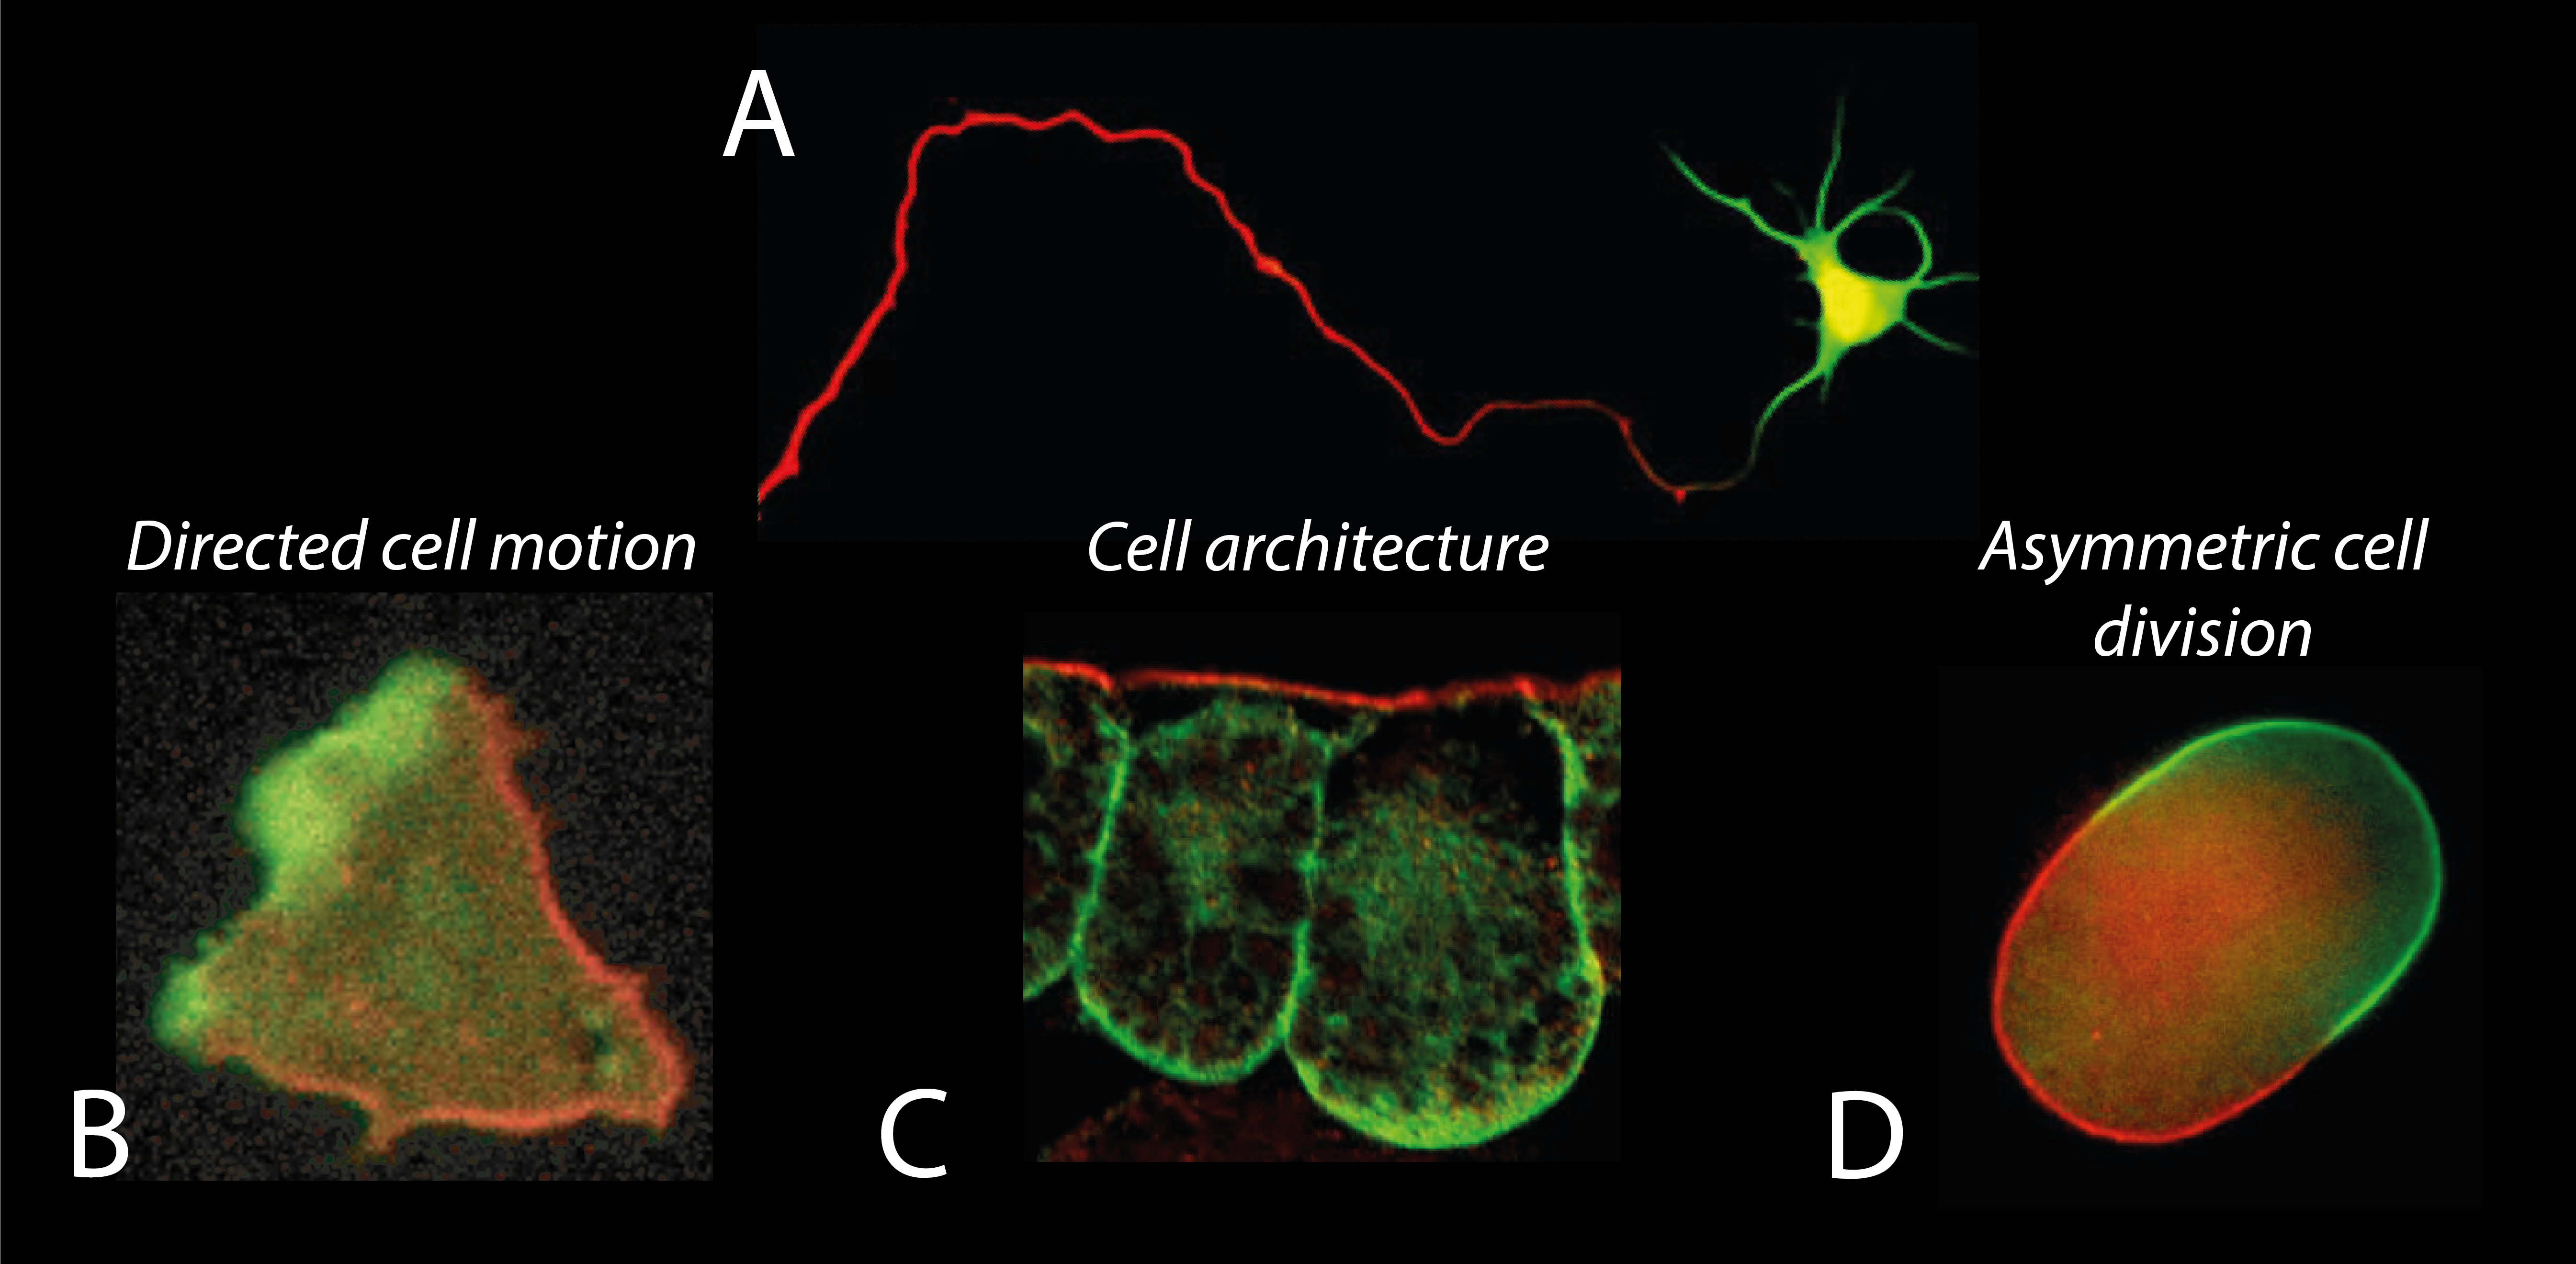
\includegraphics[scale=1.1]{polarity_examples}
\centering
\mycaption{Examples of cell polarity}{
\textbf{(A)} A neuron, which is polarised to send signals from an input end to an output end.
\textbf{(B)} A \textit{Dictyostelium} cell, which is polarised to move in a certain direction.
\textbf{(C)} Epithelial cells are polarised along an apico-basal axis. An apical surface faces the exterior of a tissue or a lumen (e.g. for uptake of nutrients) and a basal surface contacts a basement membrane.
\textbf{(D)} A \textit{C. elegans} zygote, which polarises prior to an asymmetric cell division.
Red and green represent the localisation of different polarity proteins.
}
\label{fig:cell_polarity_examples}
\end{figure}

Polarity is a property that applies to nearly every cell that one might come across. Epithelial cells (\cref{fig:cell_polarity_examples}C) are another example, where an axis is coordinated to perform roles such as directional nutrient uptake. Migrating cells are polarised to allow them to move in a certain direction (\cref{fig:cell_polarity_examples}B). A final example (and of particular relevance to this project) is seen in dividing cells, where asymmetries in a mother cell ensure that the two daughter cells are different from one another (\cref{fig:cell_polarity_examples}D).\\

In all cases, polarity arises due to a series of orchestrated rearrangements of cellular components. Directed cell motion, for example, involves rearrangements of the contractile cytoskeleton along a certain axis. Asymmetric cell divisions generally involve the movement of fate determinants and the cell division machinery towards one end of the mother cell. \\

This begs the ultimate question of how such asymmetries arise in the first place. The diversity of contexts might suggest that many distinct mechanisms are at play. Remarkably, however, whilst some of the molecular details do differ between systems, many of the core mechanisms are conserved between systems.\\

In most cases, cell polarisation is driven by small networks of molecules, known as polarity proteins, that self-organise to form polarised patterns on the plasma membrane of cells (these are highlighted in green and red in \cref{fig:cell_polarity_examples}). Once in these arrangements, these proteins act as master regulators of cell polarity, driving a series of downstream processes to set up functional asymmetries in cells.\\

A particularly important set of proteins in this regard is the PAR network, which regulates polarity across metazoa in a range of contexts, such as epithelia and stem cells. A broad, interdisciplinary field of research has emerged aiming to understand what these proteins are, how they regulate the downstream processes of cell polarity and, perhaps most importantly, how they become polarised in the first place.\\



\subsection{The PAR network}
% Rukshala 1.2.2
% Jake 1.2.1

The PAR proteins (table \ref{tab:par_proteins}) were first identified in \textit{C. elegans} in screens of mutants that disrupt asymmetric zygote divisions \citep{Kemphues1988, Morton2002, Watts1996}. In this particular context, it was later shown that a subset of these proteins becomes enriched asymmetrically at the cell cortex in distinct anterior and posterior domains (as seen in \cref{fig:cell_polarity_examples}D). Once in this distribution, the PAR proteins then direct an asymmetric cell division by controlling both the segregation of fate determinants and asymmetric positioning of the cleavage plane \citep{Rose2014}. When the zygote divides, these asymmetries result in the formation of two cells that differ in size and eventual fate.\\

\begin{table}[]
\footnotesize
\begin{tabular}{|llll|}
\hline
Name & Description & Drosophila homologue & Mammalian homologue \\ \hline
PAR-1 & Kinase & Par-1 & MARK kinases \\
PAR-2 & RING protein & Not conserved & Not conserved \\
PAR-3 & Scaffold protein & Bazooka & mPar3 \\
PAR-4 & Kinase & Par4 & LKB1 \\
PAR-5 & 14-3-3 protein & Par5 & 14-3-3 proteins \\
PAR-6 & Adaptor protein & Par6 & mPar6 \\ \hline
\end{tabular}
\mycaption{The PAR proteins}{
PAR proteins identified in original screens by Ken Kempues and colleagues, details attributed to them in later studies, and homologues in other species. A range of other proteins, whilst not PAR by name, are often considered part of the PAR network due to their interactions with these proteins. In \textit{C. elegans}, this includes the kinase PKC-3, the small GTPase CDC-42, the Rho GAP CHIN-1, and the tumor suppressor LGL-1. Table adapted from \cite{Insolera2011}.
}
\label{tab:par_proteins}
\end{table}

Since their initial discovery in \textit{C. elegans}, further work has gone on to show that these proteins act to set up polarity in numerous different cell types and organisms \citep{Goldstein2007}.  Extensive research has focussed on understanding the identity and roles of the individual PAR proteins, which has shed considerable light on the mechanisms driving cell polarity. The PAR network is now known to consist of a mix of kinases, scaffolds and adaptor proteins, each of which has their own specialised role in regulating polarity \citep{Lang2017}.  The core PAR network consists of the scaffold protein PAR-3, the adaptor protein PAR-6, the kinase PKC-3, the GTPase CDC-42 and the kinase PAR-1. Depending on the system, other proteins and protein complexes interact with these core components to help set up polarity.  In epithelia, for example, the Crumbs complex (consisting of Crb, Sdt and PatJ) and the Scribble complex (consisting of Scrib, Dlg and Lgl) interact with the core PAR network to help set up apico-basal polarity \citep{Rodriguez-Boulan2014}. Another example, of particular relevance to this thesis, is the RING-domain containing protein PAR-2, a \textit{C. elegans} specific protein that interacts with PAR-1 to help set up anterior-posterior polarity in the embryo.\\

Whilst the identity of the PAR proteins is known, our understanding of how they interact to generate stable patterns in cells is far from complete. In this project, I aim to further our understanding of how the PAR proteins create polarised patterns in cells, specifically using the \textit{C. elegans} embryo as a model system. To set up the project, I will begin by giving a broad overview of the \textit{C. elegans} embryo system. I will then discuss mathematical modelling frameworks that have been instrumental in furthering our understanding of how the PAR proteins form patterns. Finally, I will give a more detailed account of the known molecular interactions in the PAR network, focussing on the \textit{C. elegans} embryo system.\\


\subsection{PAR polarity in the \textit{C. elegans} embryo}

The system in which the PAR proteins were first discovered, the \textit{C. elegans} embryo (and most commonly the one-cell zygote in particular), has continued to be an important model system for research into the PAR proteins. As large, transparent cells, \textit{C. elegans} zygotes are particularly suitable for quantitative imaging, and there are a range of genetic tools available in \textit{C. elegans} that allow researchers to readily perturb protein function. Additionally, being confined to a single cell, the system is simpler than many others, which allows for easier identification of core principles of PAR polarity that would be more difficult to uncover in complex tissues.\\

As previously mentioned, the system comprises of two groups of proteins that define distinct anterior and posterior domains. We refer to these two groups as aPARs (anterior PARs) and pPARs (posterior PARs) respectively. The anterior domain is composed of the oligomeric scaffold protein PAR-3, the adaptor protein PAR-6, the kinase PKC-3 and the GTPase CDC-42. The posterior domain is composed of the kinase PAR-1, the RING-domain protein PAR-2, the tumour suppressor LGL-1 and the GTPase-activating protein (GAP) CHIN-1. Two additional proteins, the kinase PAR-4 and 14-3-3 protein PAR-5, are not asymmetrically localised but play a role in setting up asymmetry of the other PARs.\\

The polarisation process is generally described in terms of two distinct phases: establishment phase, in which PAR asymmetries are first set up, and maintenance phase in which PAR asymmetries are maintained until cell division. Prior to the establishment phase, aPARs are uniformly enriched at the cortex, and pPARs are cytoplasmic (\cref{fig:par_polarity_schematic}i). Polarity is triggered by the sperm donated centrosome (\cref{fig:par_polarity_schematic}ii), which causes symmetry of the system to be broken via two redundant pathways. Firstly, signals from the centrosome lead to an inhibition of cortical actomyosin contractility in the posterior, triggering cortical flows that segregate aPARs to the anterior \citep{Munro2004, Goehring2011a}. Secondly, microtubules associated with the sperm centrosome can directly promote PAR-2 binding to the cortex in the posterior \citep{Motegi2011, Wallenfang2000, Zonies2010}. Together, these mechanisms break the symmetry of the system, establishing an aPAR rich anterior and a pPAR rich posterior. \\

\begin{figure}
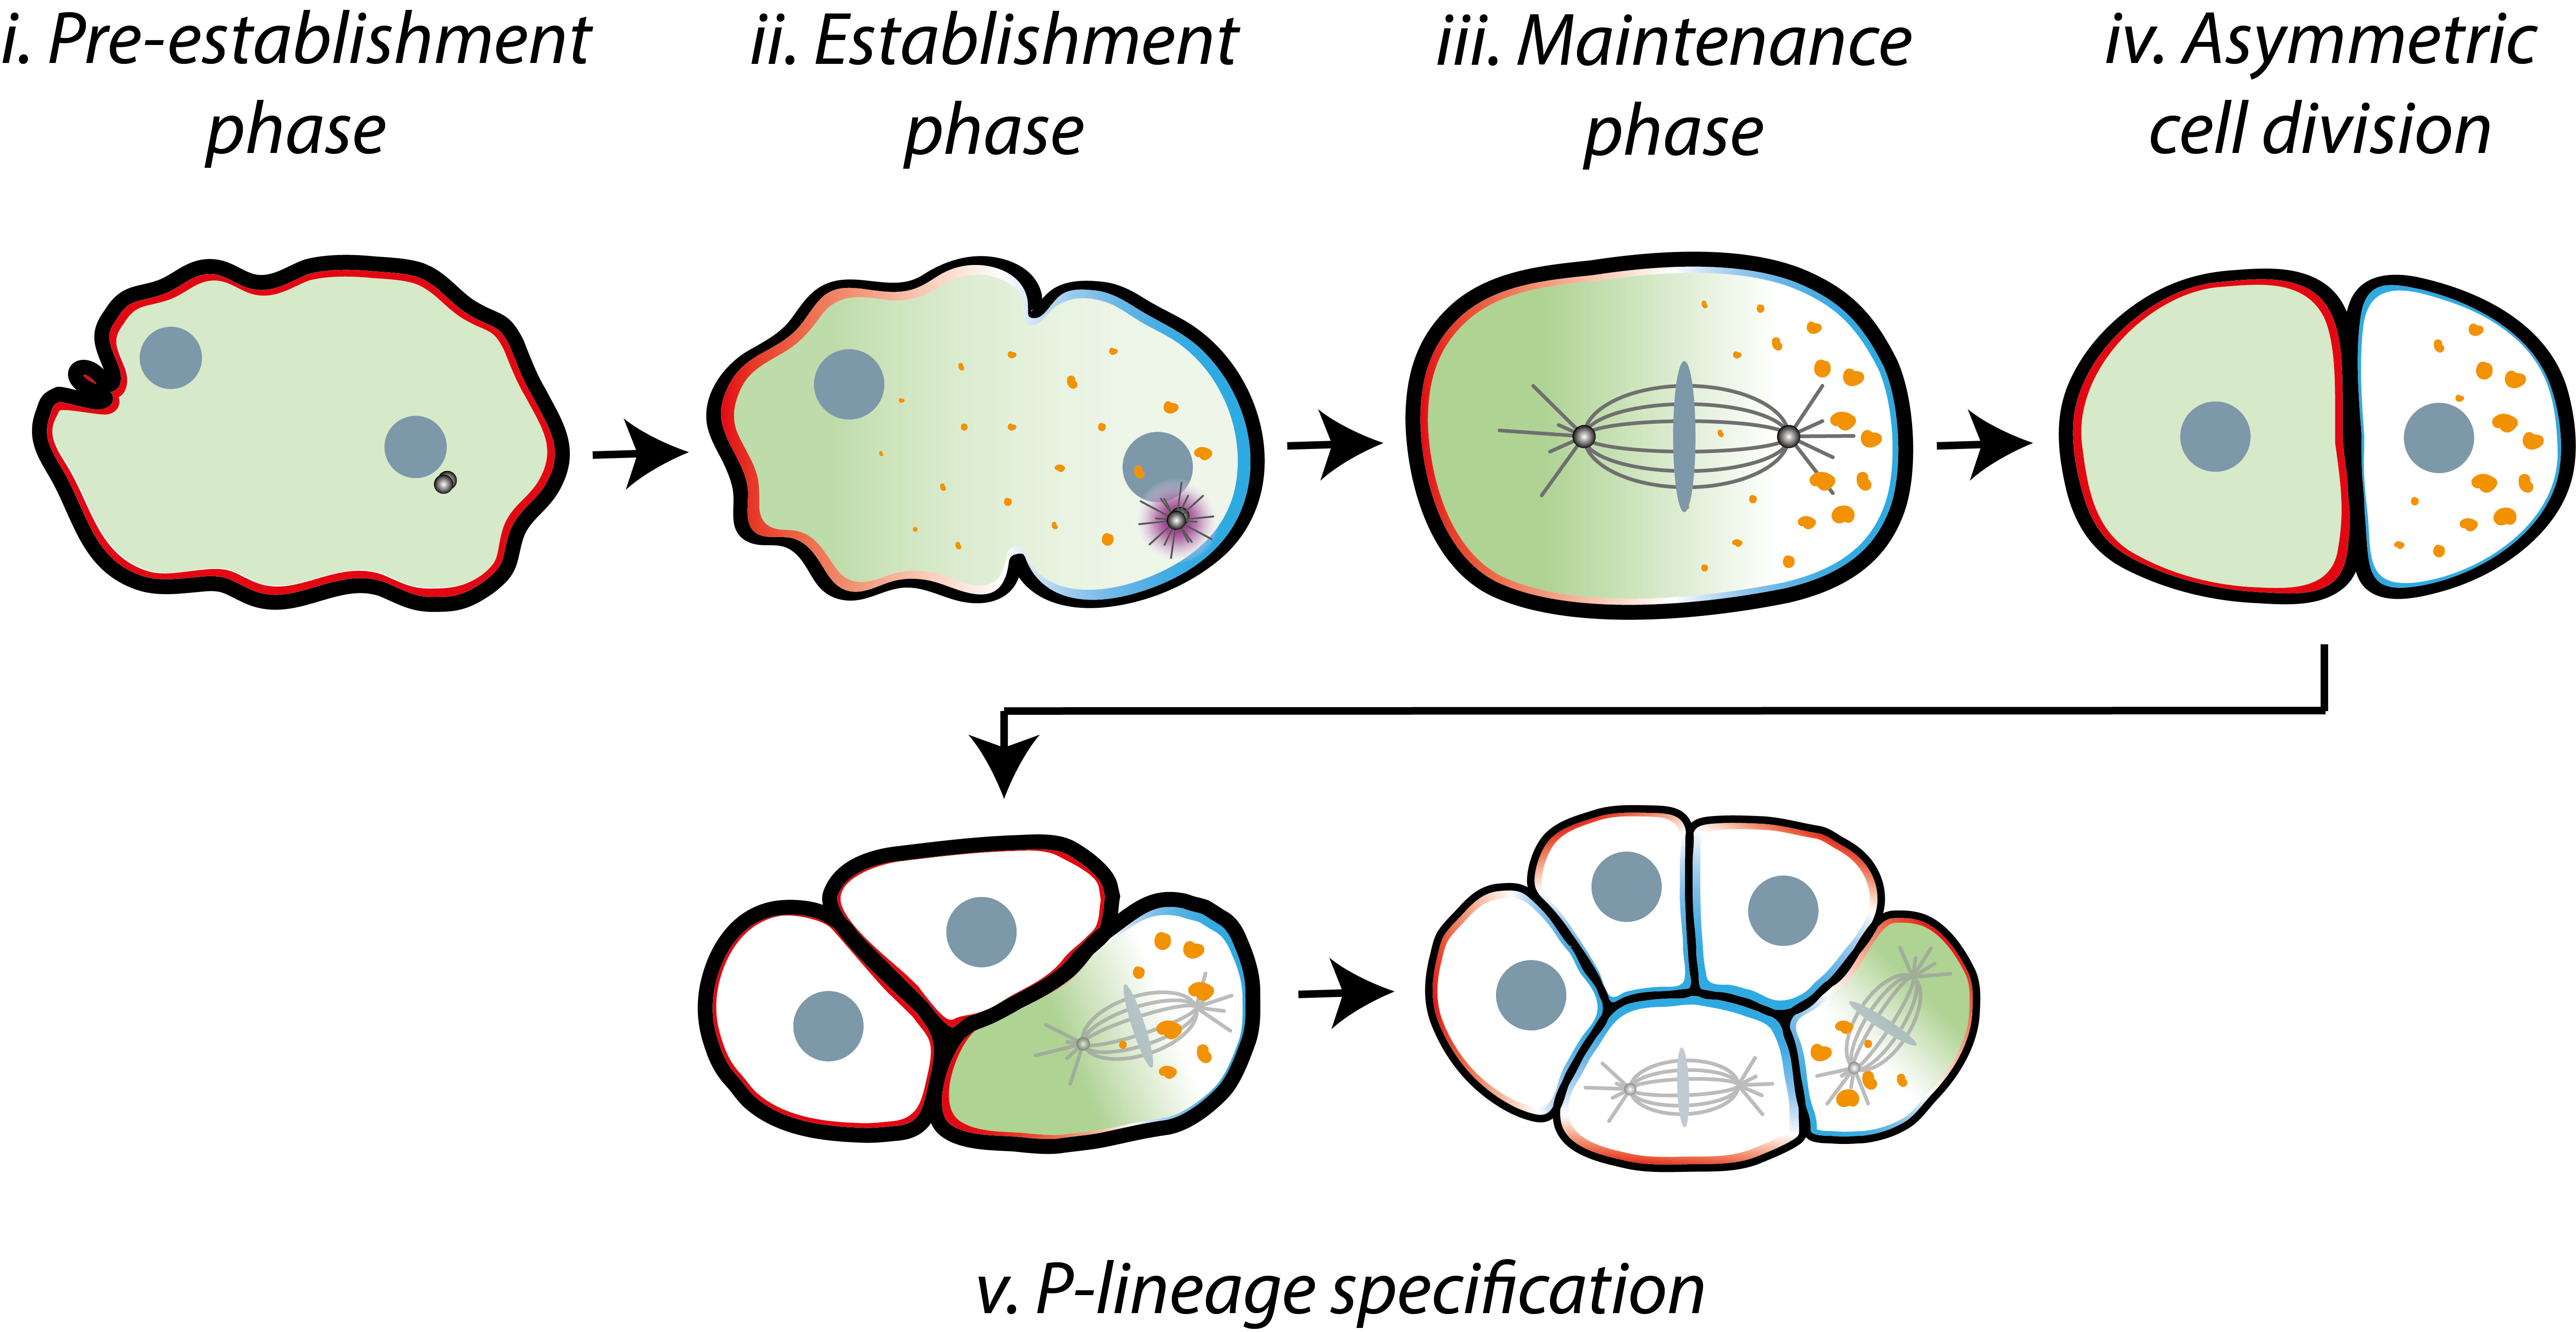
\includegraphics[scale=1]{par_polarity_schematic}
\centering
\mycaption{Schematic of PAR polarity}{
\textbf{(i - ii)} Starting from an initial state in which aPARs (red) are uniform on the cortex and pPARs (blue) are cytoplasmic, a cue from the sperm centrosome (purple) promotes aPAR movement towards the anterior and pPAR loading at the posterior to set up polarity along an anterior-posterior axis. 
\textbf{(iii)} PAR domains are then maintained until cytokinesis, and drive polarity of cytoplasmic factors such as MEX-5/6 (green) and germline fate-determinants (orange), as well as asymmetric spindle localisation.
\textbf{(iv)} The cell divides to give two cells with distinct size and fate.
\textbf{(v)} This process then repeats throughout the P-lineage in a series of smaller cells, eventually restricting germline fate to a pair of founder cells. 
Adapted from figure by Nate Goehring.}
\label{fig:par_polarity_schematic}
\end{figure}

After polarity is established, cortical flow velocities are markedly reduced \citep{Gross2018}, and the sperm centrosome moves the centre of the cell, where it will help set up the mitotic spindle. Nevertheless, despite this loss of spatial cues from the system, aPAR and pPAR domains are able to remain stable and keep their axis of polarity until cytokinesis (\cref{fig:par_polarity_schematic}iii).\\

Rather than relying on spatial cues, the polarity maintenance phase is thought to reflect a dynamic steady-state, involving continuous exchange of proteins between the cortex and cytoplasm, diffusion, and protein-protein interactions \citep{Goehring2011}. Especially important are a set of antagonistic interactions between the aPAR and pPAR proteins, known as mutual antagonism, which prevents domains from mixing. In support of this view, pPAR proteins are known targets of PKC-3 and their phosphorylation is sufficient to displace them from the membrane \citep{Hao2006, Hoege2010}. Similarly, PAR-1 and CHIN-1 can inhibit the activity of PAR-3 and CDC-42, respectively \citep{Sailer2015}. Moreover, if either set of PAR proteins is disrupted, the other set of proteins localises uniformly on the cortex and polarity is lost, highlighting the essential competitive nature of the interactions between the two groups \citep{Etemad-Moghadam1995, Boyd1996, Cuenca2003, Guo1995}.\\

Signalling from asymmetric PAR proteins leads to asymmetric segregation of cell fate determinants \citep{Cuenca2003, Daniels2010, Griffin2011, Wu2018} and asymmetric placement of the cleavage plane \citep{Grill2001}. The net result is an asymmetric cell division (\cref{fig:par_polarity_schematic}iv), with daughter cells differing in both size and fate. This process then repeats in subsequent cell divisions, playing an essential role in early patterning of the embryo (\cref{fig:par_polarity_schematic}v). \\

To understand how interactions between the PAR proteins can lead to the stable maintenance of polarised patterns, researchers are increasingly making use of mathematical models to simulate the network. The system has hallmarks of a self-organising reaction-diffusion system, a phenomenon that applies not only to cell polarity, but has been hugely influential for understanding biological patterning more broadly. In the section below I will introduce the concept of self-organisation, and discuss applications of this theory to cell polarity research.\\



\clearpage
\section{Patterning via self-organisation}

\subsection{Principles of self-organisation}

The notion of self-organisation was first put forward by Alan Turing in his seminal 1952 paper `The Chemical Basis of Morphogenesis' \citep{Turing1952}. In this paper, Turing showed that diffusion of molecules, coupled to feedback reactions (in which the molecules themselves regulate their own local accumulation) is sufficient to spontaneously induce pattern formation from a uniform system with stochastic fluctuations.\\

Later work by Gierer and Meinhardt formalised this theory in a more intuitive framework, and emphasised a number of core principles that are required for reaction-diffusion systems to form patterns \citep{Gierer1972}. They proposed that a minimal patterning system requires at least two species that diffuse at different rates, one of which (the slowly diffusing species) must act to locally enhance its own concentrations (local amplification). At the same time, a long-range inhibitory signal, mediated by the faster diffusing species, must act to confine amplification of the first species to a local region (long-range inhibition).\\

Local amplification may be direct (\cref{fig:feedback_modes_schematic}, autocatalysis), via two negative reactions (\cref{fig:feedback_modes_schematic}, mutual antagonism), or via more complicated pathways involving multiple species. Long-range inhibition can be achieved in multiple ways, such as activator-inhibitor systems and activator-depletion systems (\cref{fig:activator_inhibitor}). \\

\begin{figure}
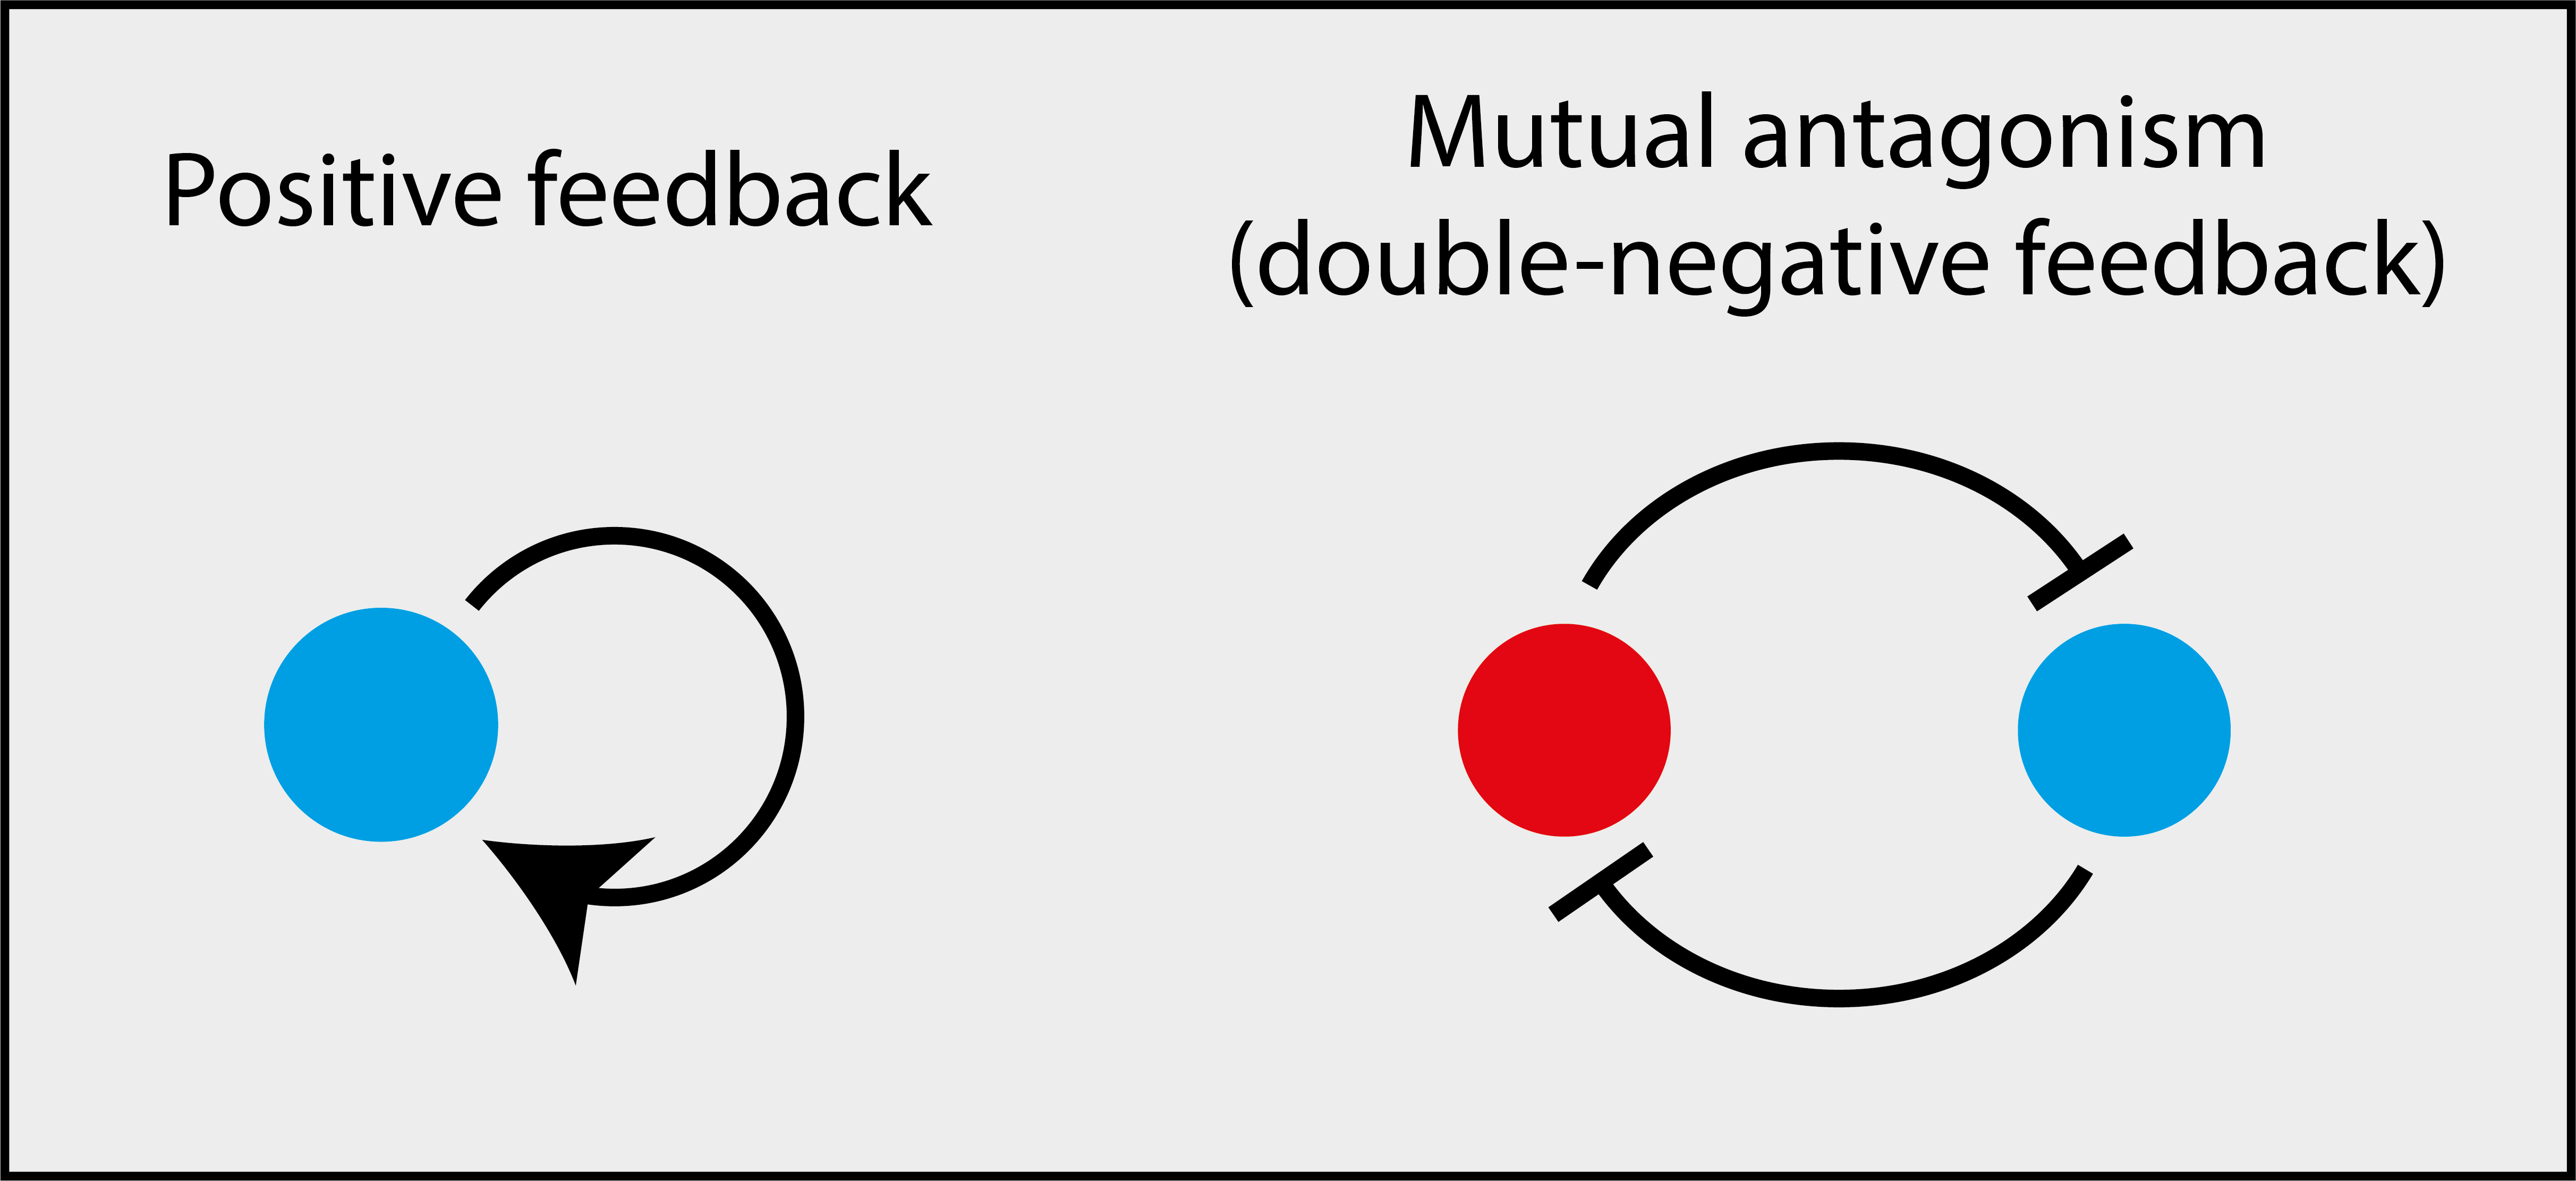
\includegraphics[scale=1]{feedback_modes_schematic}
\centering
\mycaption{Schematic of two modes of positive feedback: autocatalysis and mutual antagonism}{
In an autocatalytic mechanism, a species acts to positively regulate its own accumulation, which leads to positive feedback. In a mutual antagonism reaction, two species inhibit each other's local accumulation. This sets up a double negative feedback reaction, which is functionally equivalent to positive feedback \citep{Ferrell2002}. 
}
\label{fig:feedback_modes_schematic}
\end{figure}

\begin{figure}
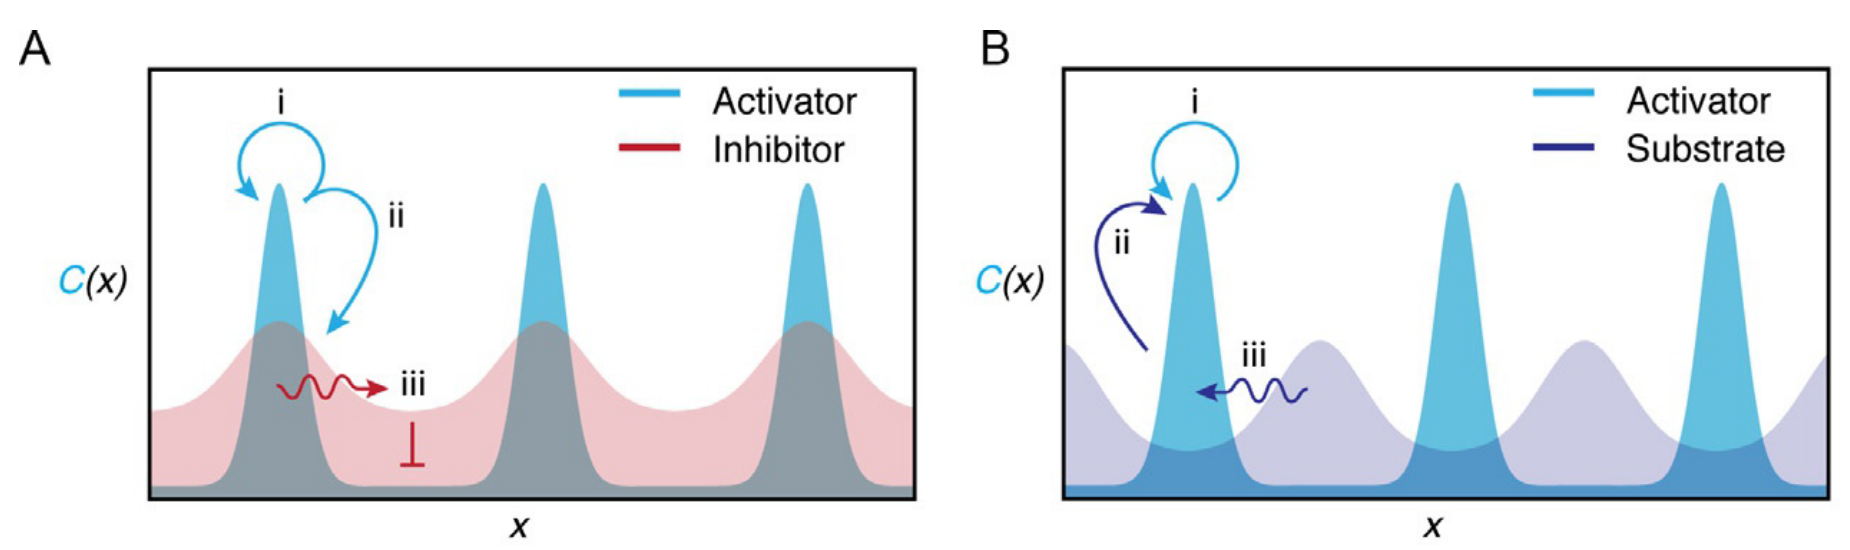
\includegraphics[scale=0.4]{activator_inhibitor}
\centering
\mycaption{Activator-inhibitor and activator-depletion networks}{
\textbf{(A)} Activator-inhibitor network. An activator promotes its own local production (i), and the production of a faster-diffusing inhibitor (ii). The inhibitor spreads to suppress the peak over a characteristic length scale (iii).
\textbf{(B)} Activator-depletion network. The activator promotes its own production (i), which locally depletes available substrate (ii). Diffusion of the substrate leads to long-range depletion, which suppresses spread of the peak (iii).
Figure from \textcite{Hubatsch2019}.
}
\label{fig:activator_inhibitor}
\end{figure}


The core ideas of Gierer and Meinhardt’s models are general, and can be applied to explain patterns across biology. One can interpret the chemical species as diffusing across tissues, controlling gene expression, and interacting to set up patterns of gene expression. In this way, these models can create 2D patterns that very much resemble the patterns one might see on the skin of an animal (\cref{fig:gierer_meinhardt}), and a whole range of other patterns are possible. One could even replace the description of diffusing chemicals with a description of neural activity. In this way, similar models can explain the development of patterned neural connections in the nervous system \citep{Willshaw1976}. Finally, and as discussed in the next section, these principles are also readily applied to the context of an individual cell.\\

\begin{figure}
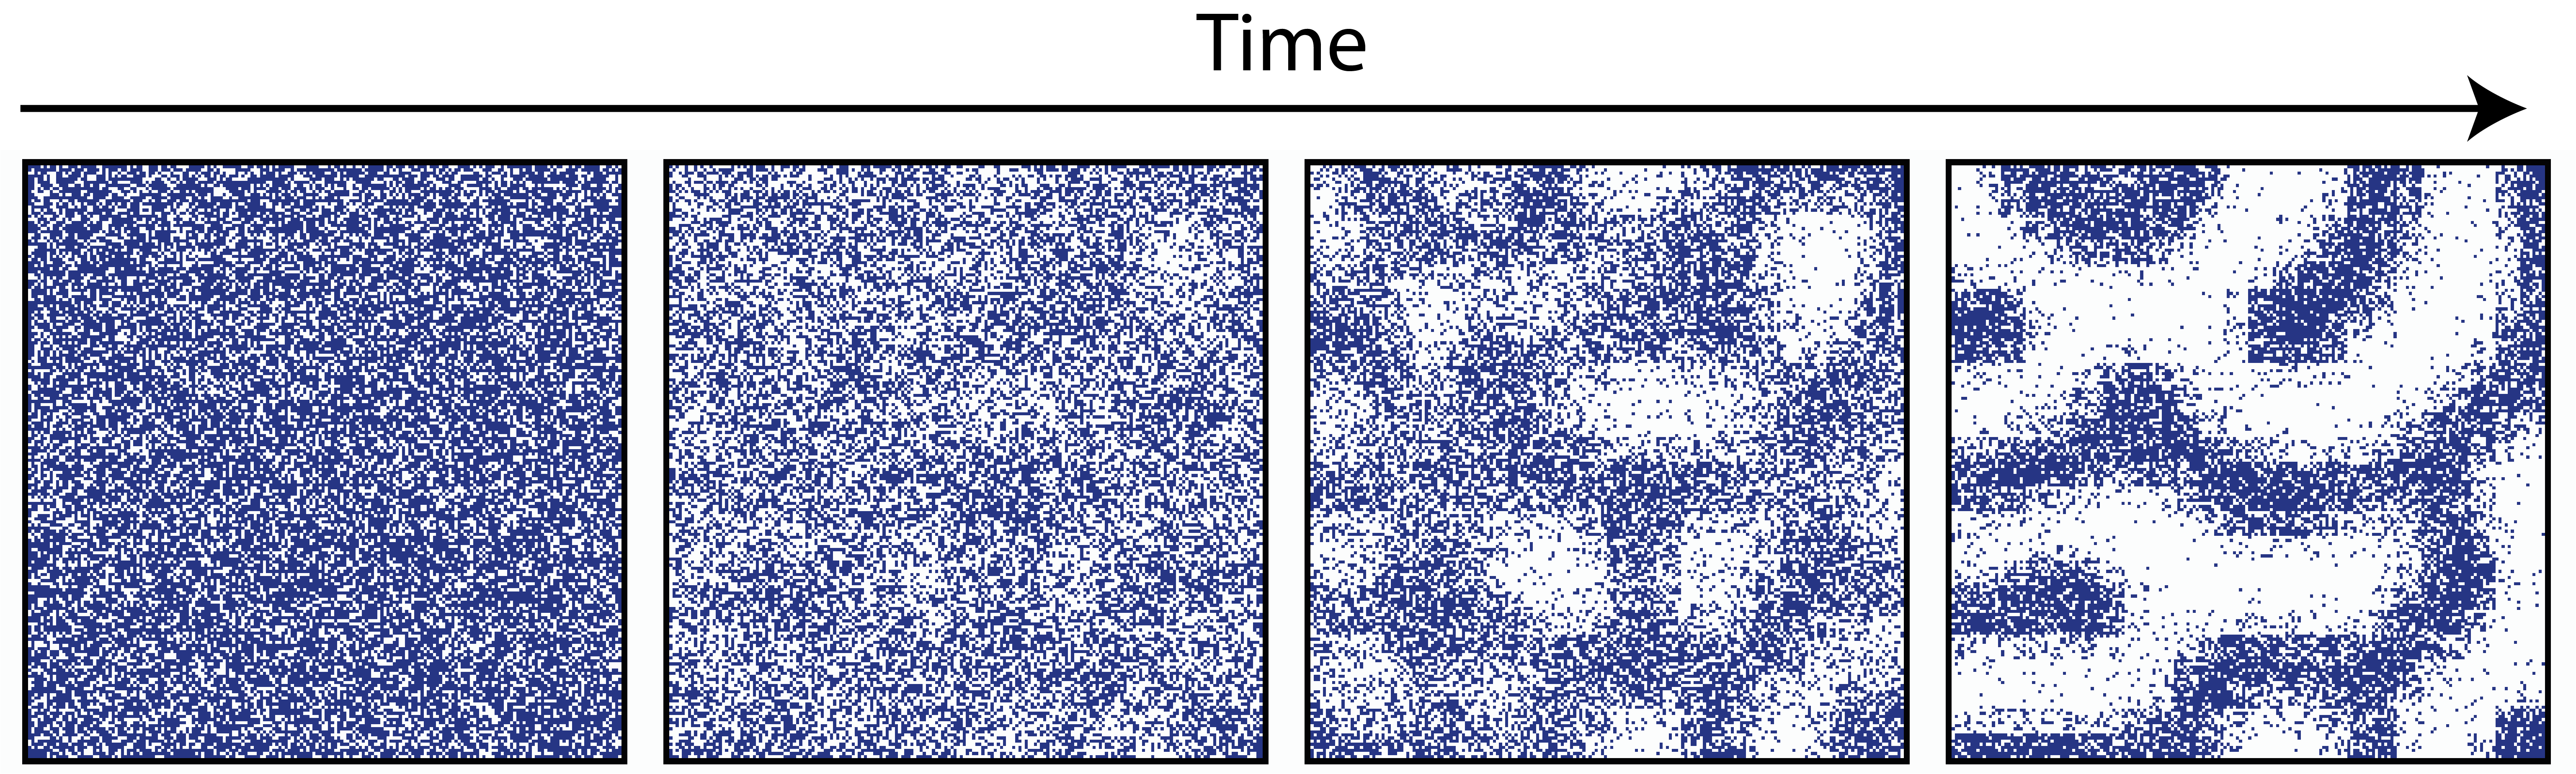
\includegraphics[scale=1]{gierer_meinhardt}
\centering
\mycaption{An example of pattern formation in the Gierer-Meinhardt model}{
Starting from an initial uniform state with stochastic variation, the system spontaneously amplifies local fluctuations and self-organises into a stable pattern. Figure adapted from \textcite{Meinhardt2006}.}
\label{fig:gierer_meinhardt}
\end{figure}

\clearpage
\subsection{Self-organisation for cell polarity}

Using these core principles, a number of models have been proposed to describe cell polarity. For the most part, models do not attempt to address the complex biochemistry of cell polarity networks, but compose systems as a small number of species and core reactions. Species in models generally do not refer to a single protein but to a set of proteins that interact together. Feedback reactions, which are generally complex, multi-step reactions in vivo are built as single (or a small number) of mass-action reaction terms in differential equations. Because polarisation often occurs over a single axis, systems are usually modelled in one-dimension.\\

Some polarity models are considered `Turing-type', characterised by instabilities that cause systems to react to small spatially varying stimuli and spontaneously break symmetry (e.g. \cite{Otsuji2007, Goryachev2008}). These are attractive in the sense that they can account for spontaneous polarisation and can achieve high degrees of spatial asymmetry. However, they generally fail to account for resting nonpolar states which are often observed in vivo, in which systems wait for a sufficiently large trigger before polarity is initiated.\\

A second class of models relies on bistable reaction kinetics driven by nonlinear feedback reactions to produce `wave-pinning' behaviour \citep{Jilkine2011, Mori2008, Mori2011}. Unlike classic Turing instability models, in which small perturbations are always amplified, the model permits parameter regimes in which unpolarised rest states are stable to small stimuli and stochastic fluctuations. Systems in these parameter regimes will not break symmetry spontaneously, and require a sufficiently large trigger to initiate polarity.
(Note, this is parameter dependent, and these models generally also permit parameter regimes which display `Turing-type' unstable behaviour \citep{Trong2014})\\

In this section I will describe two models that are particularly relevant to this work. I will first describe the original wave-pinning model, a simple model that shares many conceptual features with models of the PAR network (although the precise mechanisms are quite different), before moving onto a minimal model of PAR polarity.\\


\subsubsection{Wave pinning model}

The wave-pinning model is a minimal cell polarity model that was initially motivated to describe patterning of RhoGTPases, a conserved family of polarity proteins that regulate cell polarity in a range of contexts and cell types. An example is budding yeast, in which asymmetric cell divisions are controlled by the RhoGTPase Cdc42, which forms a polar cap on the cell membrane (\cref{fig:yeast_polarity_schematic}A). Cdc42 exists in a continuous cycle between an active GTP-bound membrane state and an inactive GDP-bound cytoplasmic state. Switching between these two states is catalysed by two classes of proteins. The guanine nucleotide exchange factor (GEF) Cdc24 switches Cdc42 to its active state, and a group of GAPs switch Cdc42 to its inactive state. Another key player is the scaffold protein Bem1, which is recruited to the membrane by the active form of Cdc42 and further recruits the GEF Cdc24. This reaction leads to a positive feedback loop, in which accumulation of active Cdc42 on the membrane leads to further accumulation, causing a membrane domain to grow. Meanwhile, growth of the domain causes the cytoplasmic pool of inactive Cdc42 to be depleted, which provides a long-range inhibitory signal and eventually stalls growth (\cref{fig:yeast_polarity_schematic}B).\\

\begin{figure}
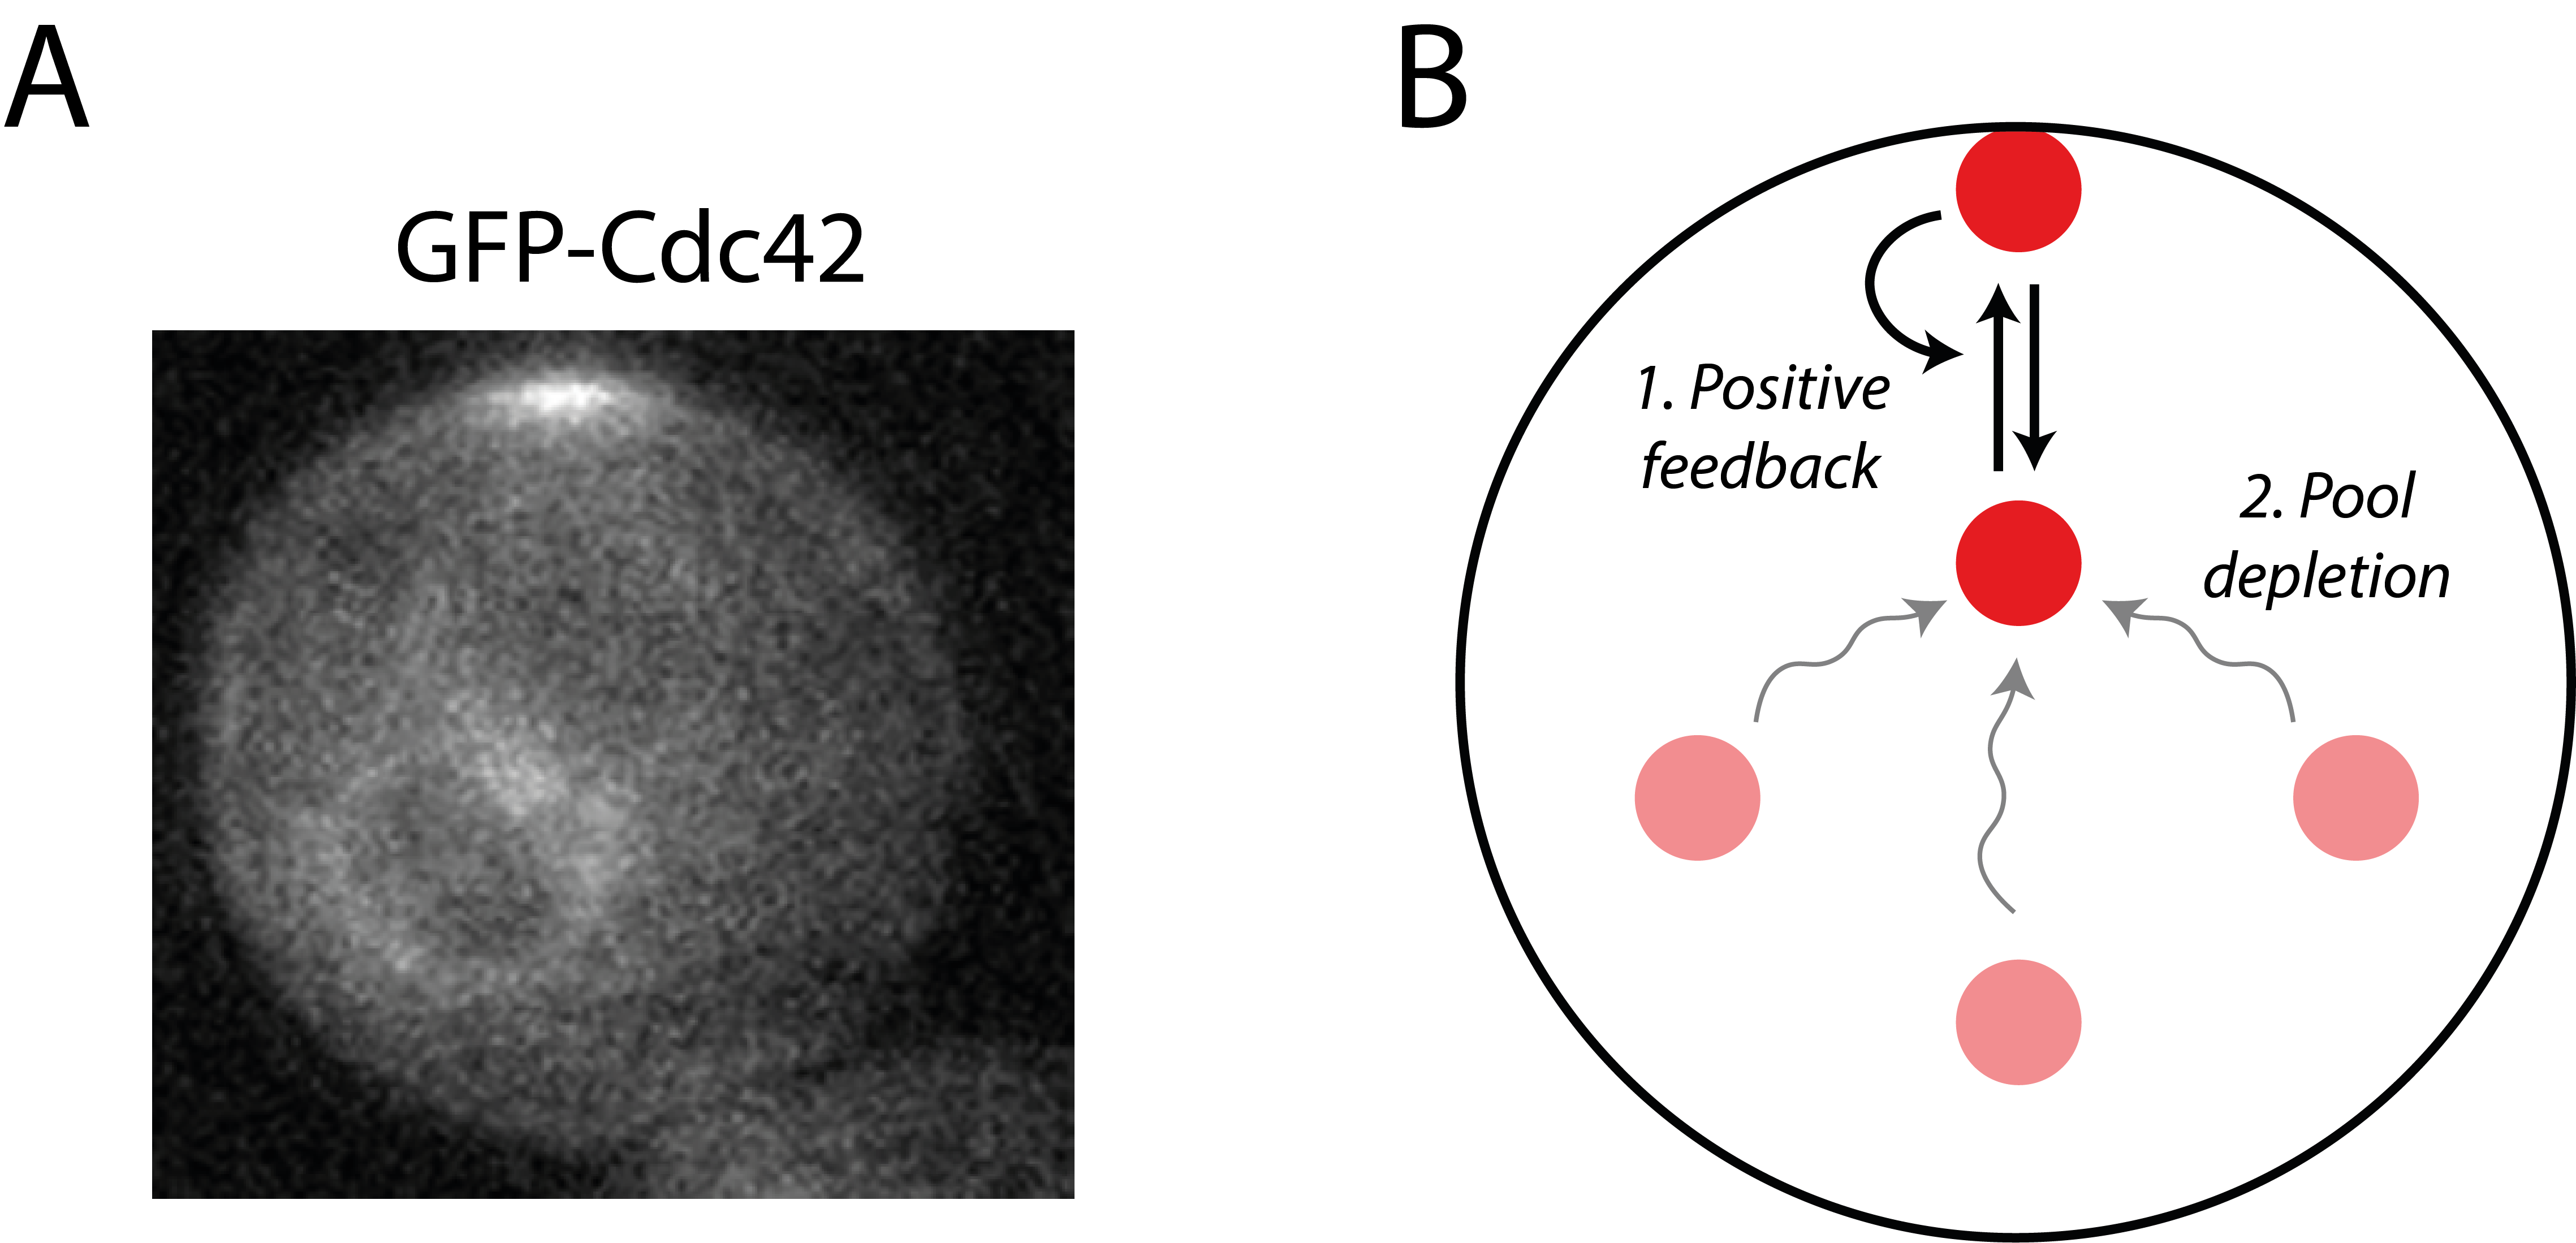
\includegraphics[scale=1]{yeast_polarity_schematic}
\centering
\mycaption{Cdc42 polarity in budding yeast}{
\textbf{(A)} A Cdc42 cap in a budding yeast cell, which marks the bud assembly site. Figure from \textcite{Klunder2013}.
\textbf{(B)} Schematic of the polarisation process, which involves positive feedback on membrane recruitment and long-range inhibition via pool depletion.
}
\label{fig:yeast_polarity_schematic}
\end{figure}

These ideas were formalised by \textcite{Mori2008} with their wave-pinning model. In this model, a single species cycles between active membrane bound ($m$) and inactive cytoplasmic ($c$) states, and the membrane state feeds back onto its own recruitment. The governing equation describing $m$ is as follows:
\begin{equation}
\frac{\partial m}{\partial t} = D_m \frac{\partial^2 m}{\partial x^2} + c \left(k_0 + \frac{\gamma a^2}{K^2 + m^2} \right) - \delta m
\end{equation}

Here, diffusion and reactions are modelled along a one-dimensional system, where $x$ is the position coordinate along a membrane around half the circumference of a cell. $D_a$ is the diffusion coefficient on the membrane. The second term in the equation describes the rate of membrane association. $k_0$ is a rate constant describing the basal rate of membrane association, and the fraction term in the brackets describes positive feedback on membrane association, which is built as a Hill function with maximum rate $\gamma$ and saturation parameter $K$. Finally, $\delta$ describes the constant rate of membrane dissociation.\\

With the assumption that cytoplasmic diffusion is fast, and so cytoplasmic concentrations are effectively uniform, $c$ can be modelled as a uniform value based on the total amount of material ($T$), according the the conservation of mass term below:
\begin{align}
c &= T - \psi \bar{m}
\end{align}

where $\bar{m}$ is the average membrane concentration and $\psi$ is the surface area to volume ratio. This assumption is a close approximation when cytoplasmic diffusion is fast, and simplifies mathematical analysis.\\

A key feature of this model is that the reaction kinetics display bistability. This can be seen by solving the reaction terms at equilibrium, which shows the permitted steady state combinations of $m$ and $c$ (\cref{fig:wave_pinning}A). We can see from this that the resulting curve folds over itself, meaning that, within a range of cytoplasmic concentrations, two stable membrane concentrations (an upper and a lower state) are permitted by the reaction terms (a third solution between them is unstable). This bistability comes as a result of nonlinearities in the reaction terms, specifically in this case the exponent of 2 in the Hill function, which implies an ultrasensitive relationship between membrane concentrations and recruitment.\\

\begin{figure}
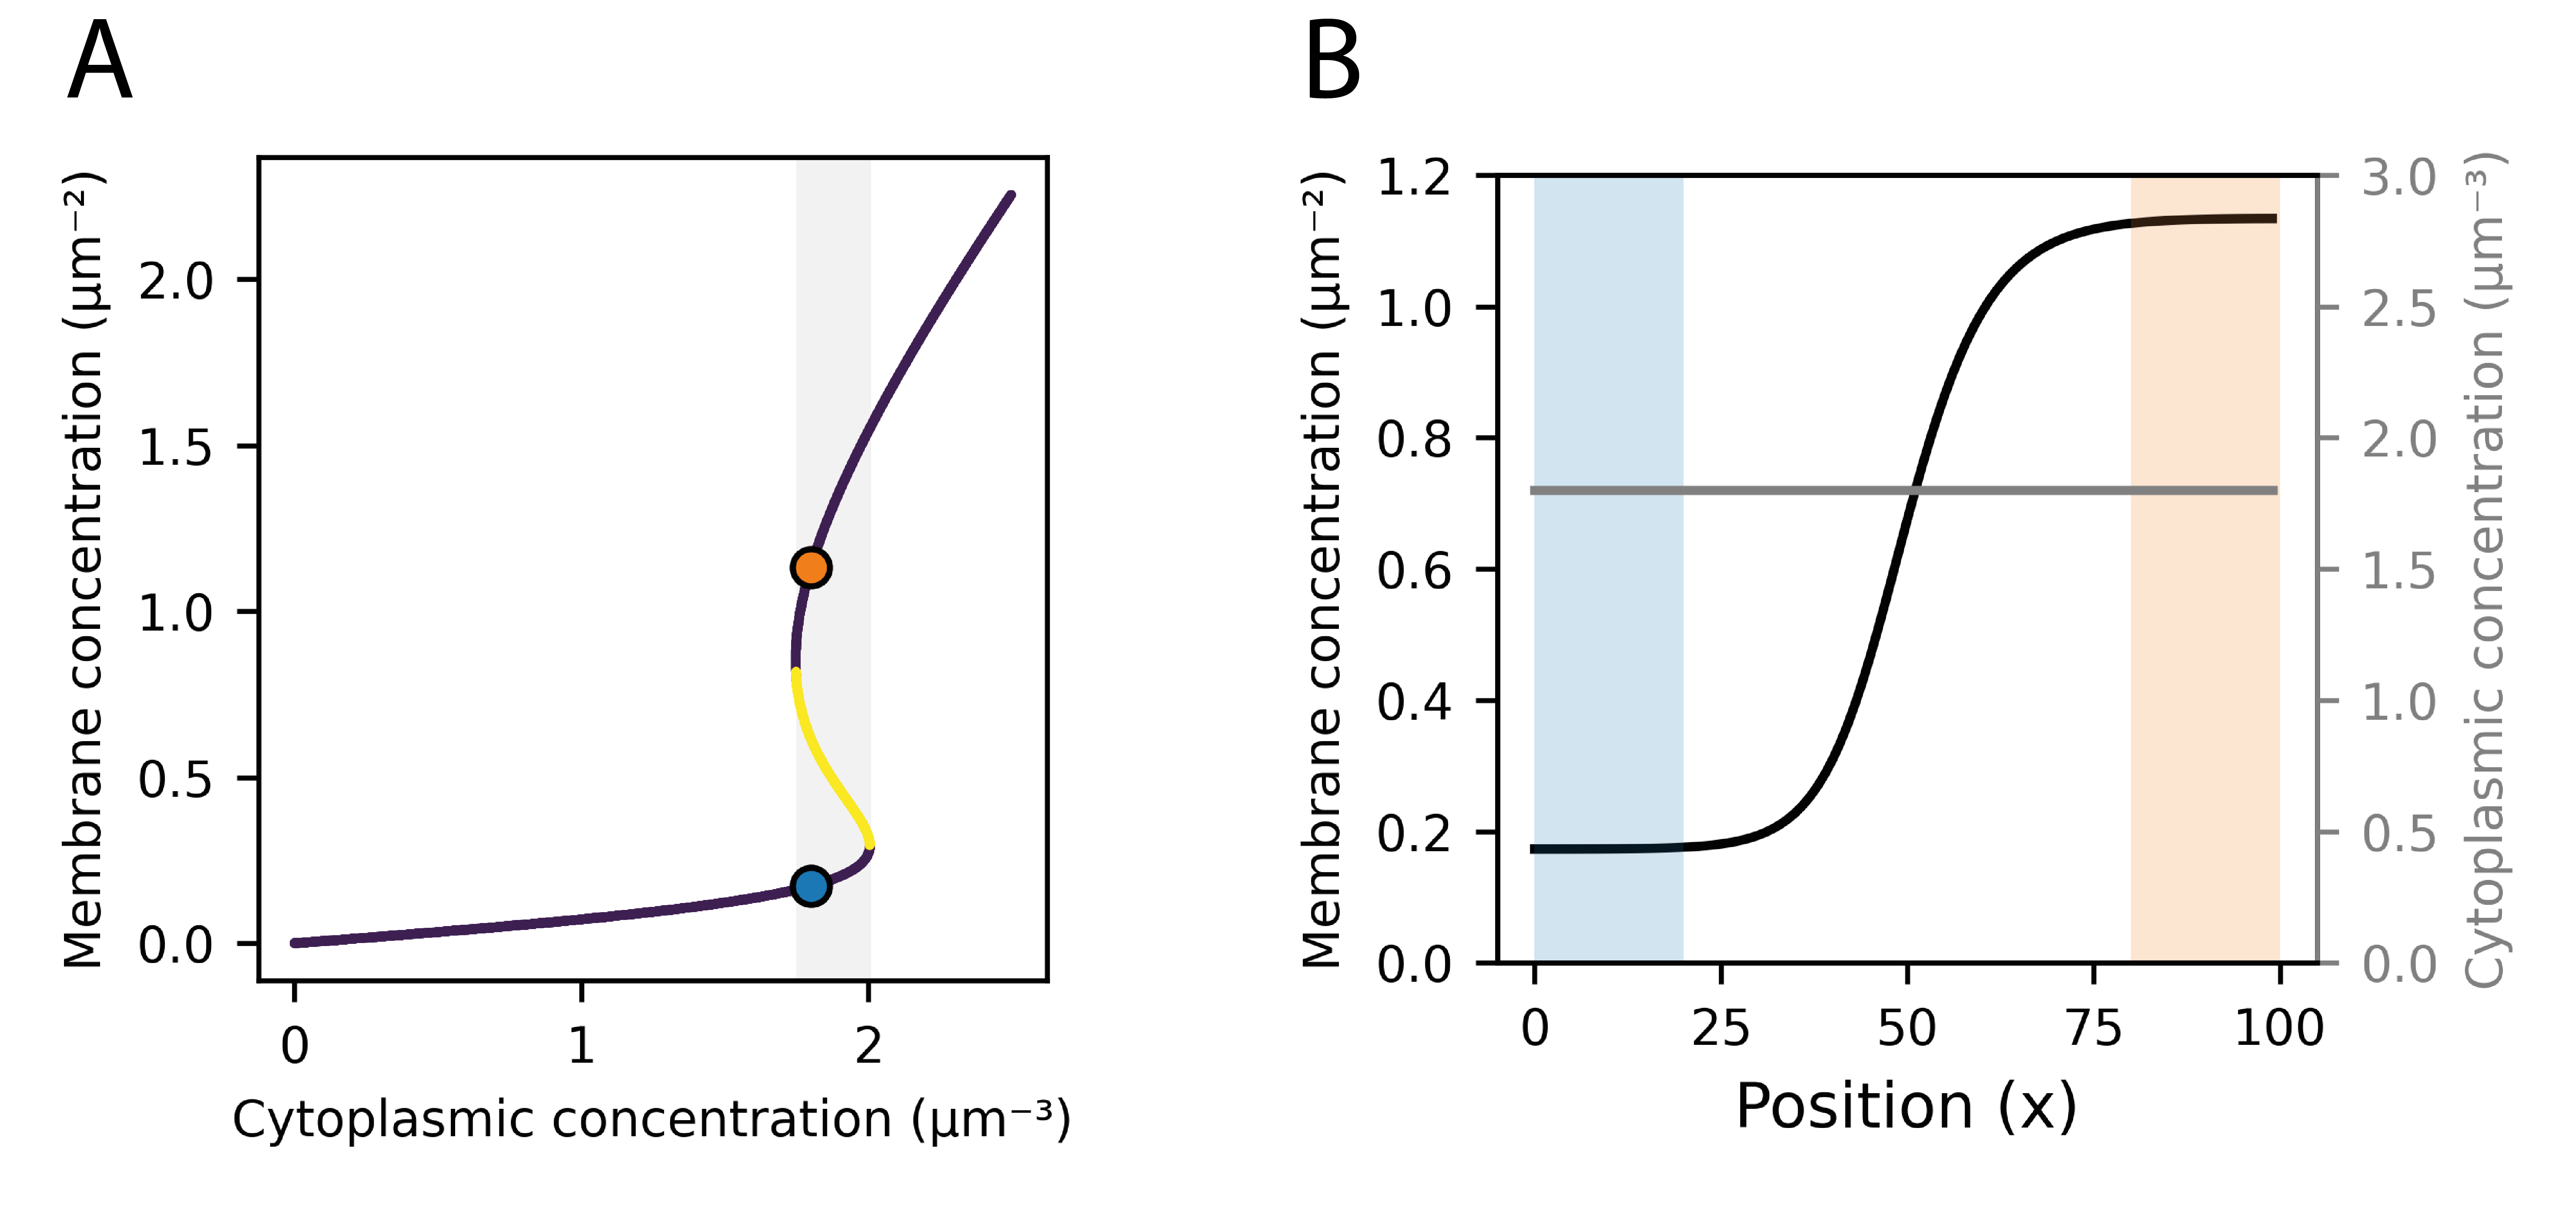
\includegraphics[scale=1]{wave_pinning}
\centering
\mycaption{Bistability in the wave-pinning model}{
\textbf{(A)} Nullcline of the solution to the wave-pinning model reaction terms. Purple indicates stable solutions along the curve, yellow indicates unstable solutions. Bistability is supported within a range of cytoplasmic concentrations (grey). Blue and orange points correspond to the two regions indicated in the pattern in B.
\textbf{(B)} Polarised pattern from a wave pinning model simulation. Given a sufficiently large trigger, the model stabilises with a polarised membrane pattern supported by a uniform cytoplasmic concentration.
Parameters: $k_0 = 0.067$, $\gamma = 1$, $\delta = 1$, $K = 1$, $D_m = 0.1$, system length = $10$, $T = 2.45$, $\psi = 1$.
}
\label{fig:wave_pinning}
\end{figure}

Starting from a uniform (lower) state, a sufficiently large transient stimulus can be locally amplified by positive feedback, bringing part of the system into the upper state. Due to diffusion, this region then spreads, until depletion of the cytoplasmic pool causes this spreading to stall (a phenomenon referred to as `wave-pinning', which gives the model its name). An example of a stable pattern is shown in \cref{fig:wave_pinning}B, which shows stable upper and lower regions separated by an interface. As pinning is caused by cytoplasmic depletion, the position of the interface is strongly influenced by the total amount of protein in the system.\\


\subsubsection{Minimal PAR model}

Rather than self-amplification, in which one protein (or group of proteins) directly feeds back onto its own local enrichment, the dominant patterning mechanism in PAR polarity is one of mutual antagonism, whereby proteins within two subgroups negatively regulate each-other's localisation. A number of attempts have been made to formalise this with mathematical models, varying in their complexity. Perhaps the simplest is a model by \textcite{Goehring2011a}. This model groups the PARs into two species, representing aPARs and pPARs. These species are in continuous exchange between membrane-bound and cytoplasmic states, which is biased by terms representing antagonism. The governing equations are as follows:\\
\begin{align}
\frac{\partial A_m}{\partial t} &= D_A \frac{\partial^2 A_m}{\partial x^2} + k_{on,A} A_c - k_{off,A} A_m - k_{AP} P_m^{\alpha} A_m\\
\frac{\partial P_m}{\partial t} &= D_P \frac{\partial^2 P_m}{\partial x^2} + k_{on,P} P_c - k_{off,P} P_m - k_{PA} A_m^{\beta} P_m
\end{align}

where $x$ is the position coordinate along a one-dimensional membrane, $D_A$ and $D_P$ are diffusion coefficients at the membrane, $k_{on,A}$ and $k_{on,P}$ are binding rates from the cytoplasm to the membrane, $k_{off,A}$ and $k_{off,P}$ are the detachment rates from the membrane to the cytoplasm, and $k_{AP}$ and $k_{PA}$ describe antagonism rates. A schematic is shown in \cref{fig:goehring_model_schematic}A.\\

With the assumption that cytoplasmic diffusion is fast, and so cytoplasmic concentrations are effectively uniform, the cytoplasmic concentrations of A and P ($A_c$ and $P_c$) can be calculated based on the total amount of material ($A_{tot}$ and $P_{tot}$) according the the conservation of mass terms below:
\begin{align}
A_c &= A_{tot} - \psi \bar{A_m}\\
P_c &= P_{tot} - \psi \bar{P_m}
\end{align}

\begin{SCfigure}
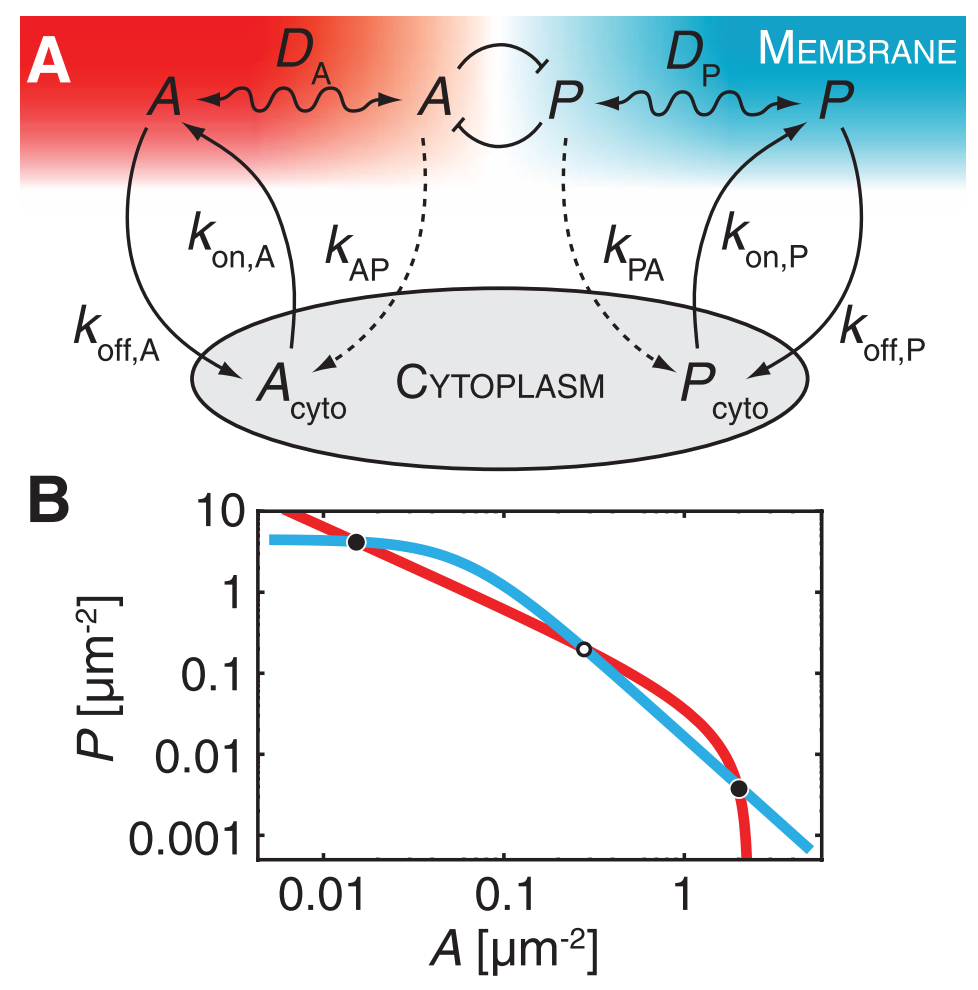
\includegraphics[scale=0.45]{goehring_model_schematic}
\centering
\mycaption{Features of the mutual antagonism model}{
\textbf{(A)} Schematic of the model. aPARs (A, red) and pPARs (P, blue) diffuse on the membrane and exchange with a well-mixed cytoplasm. Antagonistic interactions at the domain interface keep the two domains separate. 
\textbf{(B)} Nullclines of the the reaction terms with fixed cytoplasmic concentrations reveals bistability, in which the system supports two stable solutions (black) and one unstable solution (white).
Figure from \textcite{Goehring2011a}.
}
\label{fig:goehring_model_schematic}
\end{SCfigure}

Several features of the model are conceptually very similar to the wave-pinning model described previously. Nonlinearity included in the antagonism terms (either $\alpha$, $\beta$, or both must be greater than 1) give the system bistability (\cref{fig:goehring_model_schematic}B), meaning that uniform states in which either A or P dominate are stable. A sufficiently large trigger can switch the system to a polarised state in which each of these states occupy distinct ends of the cell. Depletion of the cytoplasmic pool is responsible for stabilising the boundary position, and models without this feature have an unstable polarity boundary that is prone to drift \citep{Dawes2011}.\\

The non-linearity that is required for bistability could, in theory, be achieved in a number of ways \citep{Ferrell2014a, Ferrell2014b, Ferrell2014}, and several mechanistic details of the PAR network give justification to this. One example is multisite phosphorylation \citep{Serber2007}, which is common to many targets of PKC-3, including LGL-1 \citep{Graybill2014} and PAR-2 \citep{Hao2006}. In mathematical models, the non-linearity of such reactions can be enhanced through the presence of cooperativity between phosphorylation sites \citep{Gunawardena2005}, or the presence of redundant sites \citep{Wang2010}, giving switch-like behaviour. Alternatively, oligomerisation of proteins, coupled to antagonism, has been shown to provide sufficient non-linearity to support bistability \citep{Sailer2015, Dawes2011, Lang2022}. Such reactions have been proposed for PAR-2 \citep{Arata2016},  PAR-3 \citep{Li2010a} and CHIN-1 \citep{Sailer2015}. I will discuss mechanistic details relating to these ideas further in the next section. \\


\clearpage
\section{The molecular circuitry of the PAR network}

The PAR model in the previous section describes a system in which proteins are in exchange between the cytoplasm and membrane, and feedback reactions between the two groups of proteins drive polarity maintenance. Here, I will give an overview of the molecular details thought to underlie these processes in vivo. I will begin by discussing mechanisms of cortical association. I will then discuss how this association is biased to set up polarised domains, firstly by cues which initiate polarity establishment, and secondly by antagonistic feedback reactions. Finally, I will discuss the downstream roles of these proteins that drive an asymmetric cell division. It is worth noting that the detailed mechanisms vary somewhat between different organisms and cell types, and I will focus on mechanisms of relevance for the \textit{C. elegans} embryo, although some of the studies cited were performed using other model systems.\\

\begin{figure}
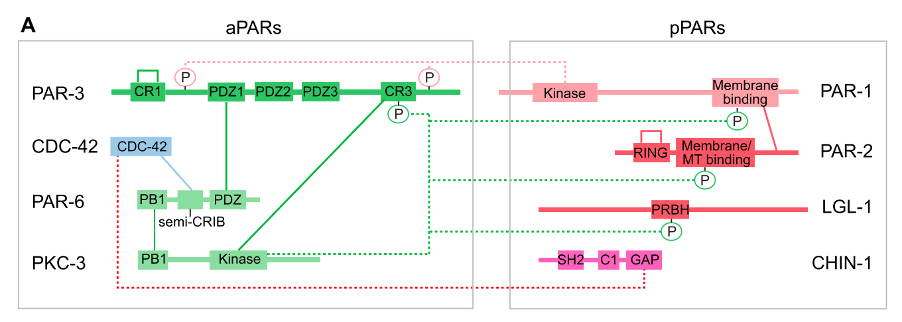
\includegraphics[scale=0.9]{par_proteins_schematic}
\centering
\mycaption{Schematic of core molecular interactions in the PAR network}{
Solid lines indicate direct binding. Dotted lines represent enzymatic activity. From \textcite{Lang2017}.}
\label{fig:par_proteins_schematic}
\end{figure}

\subsection{Mechanisms of cortical association}

The PAR proteins associate with the cortex in a number of ways. Some of the PARs display direct and intrinsic cortical localisation activity (PAR-3, PAR-2, CDC-42, CHIN-1, LGL-1). Some rely instead on other PARs to act as scaffolds (PAR-6), or fall somewhere in between with a mix of direct and scaffold-mediated cortical association (PAR-1, PKC-3).\\

\subsubsection{Association with lipids}

A number of the PAR proteins localise to the cortex by interacting directly with the inner leaflet of the plasma membrane. For some PAR proteins, this is mediated by interactions with specific phospholipids that are enriched at the plasma membrane, whereas other PARs rely on electrostatic interactions with the membrane via charged domains.\\

PAR-3, an aPAR scaffold protein, associates with the membrane via the second of its three PDZ domains \citep{Li2010a}. PDZ domains most commonly recognise C-terminal sequences on proteins \citep{Tonikian2008} or other PDZ domains, however the PDZ2 domain of PAR-3 is thought to interact directly with plasma membrane phosphoinositides \citep{Wu2007}.\\

The membrane localisation of CDC-42 is largely due to a c-terminal geranylgeranyl moiety \citep{Ziman1993}, which promotes hydrophobic attachment to cell membranes. The protein additionally contains a conserved cluster of positively charged residues directly preceding the geranylgeranyl moiety, including a di-arginine motif which promotes specificity for PIP$_2$ containing membranes \citep{Johnson2012}. This is likely responsible for the CDC-42's plasma membrane specificity.\\

Cortical localisation of PAR-2 in vivo depends on a central unstructured region of the protein rich in basic and hydrophobic amino acids \citep{Hao2006}. Full-length PAR-2 displays an ability to bind to an array of negatively charged phospholipids in vitro, suggesting an electrostatics-based interaction rather than specific interaction with any one phospholipid \citep{Motegi2011}. Given this promiscuous nature, its apparent specificity for the plasma membrane in vivo is poorly understood, but may be a consequence of the increased charge associated with the plasma membrane compared to other membranes \citep{Yeung2008}.\\

PAR-1 contains a C-terminal KA domain, a common membrane association domain, which can bind to membranes and (similarly to PAR-2) interact non-specifically with anionic phospholipids \citep{Moravcevic2010}. This domain has been shown to be both necessary and sufficient for cortical localisation in vivo \citep{Motegi2011}.\\

Cortical association of LGL-1 relies on a region towards the C-terminus of the protein, which is rich in positively charged amino acids and can directly bind to negatively charged membranes \citep{Visco2016}. Independent of overall membrane charge, affinity is strongest for membranes enriched in diphosphoinositides \citep{Visco2016}, which are most abundant in the inner leaflet of the plasma membrane.\\


\subsubsection{Interaction with scaffolds}

Whilst the pseudosubstrate and C1 regions of PKC-3 display intrinsic lipid binding activity \citep{Dong2020, Jones2022}, cortical association of PKC-3 in \textit{C. elegans} embryos usually relies on interactions with other PARs. PAR-6 and PKC-3 are stable binding partners, interacting via PB1 domains at the N-terminus of each protein \citep{Hirano2005}, and in normal circumstances are dependent on each other for stable cortical association \citep{Tabuse1998, Hung1999}. Proper cortical association of this complex relies on interactions with both PAR-3 and CDC-42. Interaction with CDC-42 relies on the semi-CRIB domain of PAR-6 \citep{Aceto2006}. Binding to PAR-3 is driven by an interaction between the kinase domain of PKC-3 and the CR3 domain of PAR-3 \citep{Lin2000, Soriano2016}, and through a PDZ binding motif at the C-terminus of PKC-3 that binds to the PAR-3's PDZ2 domain \citep{Holly2020}. PAR-6 can also interact with the PDZ1 domain of PAR-3 via its own PDZ domain, but this interaction does not appear to play an essential role in vivo in \textit{C. elegans} embryos \citep{Li2010}. \\

Whilst PAR-1 displays some intrinsic lipid binding activity, its cortical localisation is largely mediated by interactions with PAR-2. Again, this interaction is via the KA domain of PAR-1, which interacts with an unknown region of PAR-2 \citep{Motegi2011}. This reaction leads to local recruitment of PAR-1 by PAR-2, and cortical localisation in regions of PAR-2 enrichment. It has also been shown that the interaction between PAR-1 and PAR-2 can protect PAR-1 from phosphorylation by PKC-3, perhaps by occluding the phosphorylation site on PAR-1 \citep{Ramanujam2018}.\\


\subsubsection{Self-association and clustering}

For some PAR proteins, a key determinant for stable association is the ability to self-associate into oligomers, in some cases forming large clusters. In oligomers, independent membrane binding domains can cooperate with one another to promote a high affinity membrane binding interaction \citep{Lemmon2008}.\\

PAR-3 contains a CR1 domain at the N-terminus, an oligomerisation domain which assembles into helical filaments in vitro \citep{Feng2007, Zhang2013a}. Whilst CR1 mutants can localise to the membrane transiently, stable membrane association requires an intact CR1 \citep{Dickinson2017, Li2010a, Rodriguez2017}. Clustering via the CR1 is negatively regulated by PLK-1 phosphorylation, which conveys cell cycle dependence on PAR-3 cortical association \citep{Dickinson2017}.\\

Whilst little is known about the mechanisms of CHIN-1 cortical association, it has also been observed to localise in discrete puncta \citep{Kumfer2010}. These puncta only appear during late maintenance phase, and so it is plausible that, similar to PAR-3, self-association might be under cell-cycle control.\\

PAR-2 has also been suggested to self-associate and form clusters on the cortex \citep{Arata2016}, although the mechanistic basis of this is unclear. \\



\subsection{Establishment of polarity}

As previously mentioned, PAR polarity does not occur spontaneously, requiring a trigger so that polarity happens at the correct time and with the correct orientation. Prior to symmetry breaking, the system starts in an aPAR uniform state in which pPARs are held off the cortex by antagonistic interactions. Polarity is then triggered by signals from the MTOC (microtubule organising centre) which forms near the site of sperm entry, via two redundant pathways:\\

\subsubsection{Anterior-directed cortical flows}

Signals from the sperm-donated centrosome induce cortical flows towards the anterior of the embryo \citep{Cowan2004, Munro2004, Goehring2011a}. The cue is thought to lead to a local downregulation of RHO-1 activity, which downregulates actomyosin contractility in the posterior. This sets up a spatial gradient of contractility, which leads to anterior-directed cortical flows.\\

These flows transport PAR-3 clusters towards the anterior \citep{Dickinson2017, Rodriguez2017, Wang2017}, which also moves PKC-3. The resulting depletion of PKC-3 in the posterior relieves antagonism of pPARs, allowing them to bind in the posterior and form a nascent domain. Further work has shown that the PAR proteins themselves are able to feed back onto the actomyosin cortex, amplifying contractility asymmetries as polarity progresses \citep{Gross2018}.\\


\subsubsection{The microtubule pathway}

In the absence of cortical flows, symmetry breaking still occurs, albeit later, indicating the existence of multiple symmetry breaking mechanisms. A second triggering mechanism involves a transient interaction between PAR-2 and microtubules emanating from the sperm-donated centrosome. In cells lacking cortical flows, PAR-2 symmetry breaking occurs late, and correlates spatially and temporally with the site of MTOC-cortex contact \citep{Motegi2011}. Treatments that disrupt microtubules prevent symmetry breaking in these conditions.\\

Mechanistically, this is thought to be carried out by a direct interaction between PAR-2 and microtubules, which is thought to shield the phosphorylation sites on PAR-2 (discussed further in chapter 3), and has been shown to reduce phosphorylation by PKC-3 in vitro \citep{Motegi2011}. This creates a zone of local protection in the posterior of the cell, allowing PAR-2, and thus PAR-1, to load, kicking of self-organisation. Mutations at the microtubule binding interface on PAR-2 have a similar phenotype to treatments that disrupt microtubules.\\


\subsubsection{Additional pathways}

Additional mechanisms may underlie triggering in some circumstances. Microfabrication studies show that PAR-2 may have a preference for curved membranes. This may lead to preferential binding of PAR-2 at the poles of cells, which has been suggested to act as a symmetry breaking cue in cases where normal symmetry breaking is misregulated \citep{Klinkert2019}. The mechanistic basis for this proposed curvature sensitivity is unclear.\\

\subsection{Maintenance of polarity by mutual antagonism}

Following polarity establishment, one of the key drivers of polarity maintenance is a series of antagonistic reactions between the two PAR subgroups, which act to keep cortical domains separate. Antagonism from aPARs to pPARs is thought to be driven exclusively by PKC-3, whereas antagonism from the pPARs to the aPARs is driven by separate pathways involving PAR-1, LGL-1 and CHIN-1.\\

\subsubsection{PKC-3 pathway}

The pPAR proteins PAR-1, PAR-2 and LGL-1 contain FxR motifs, which act as high affinity PKC-3 recognition motifs \citep{Soriano2016}. Phosphorylation of these substrates by PKC-3 occurs within the regions that regulate membrane binding, adding negative charge which electrostatically repels the proteins from the membrane \citep{Bailey2015}. In the case of PAR-1, phosphorylation is at a single site within the membrane association domain, which is necessary and sufficient to exclude PAR-1 from the membrane \citep{Motegi2011}. LGL-1 phosphorylation occurs at three conserved sites, and phosphorylation at all three sites is required for full membrane displacement \citep{Graybill2014, Hoege2010}. PAR-2 has seven predicted phosphorylation sites \citep{Hao2006}, although these have yet to be verified biochemically. Phosphorylation by PKC-3 has been shown to disrupt binding of PAR-2 to phospholipids in vitro \citep{Motegi2011}. Mutation of all seven sites prevents phosphorylation in vivo, causing PAR-2 to localise uniformly to the cortex \citep{Hao2006}. I will discuss details relating to PAR-2 phosphorylation further in the appendix.\\

CHIN-1 does not have an FxR site, but is also excluded from the anterior by PKC-3 \citep{Sailer2015}. This is thought to involve direct inhibition of CHIN-1 clustering at the cortex by PKC-3, however the mechanistic basis of this is poorly understood.\\

Continuous dephosphorylation is required to counteract phosphorylation by PKC-3 and maintain an active pool of substrate. For the most part, the mechanisms of PKC-3 substrate dephosphorylation are poorly understood, although phosphatases GSP-1 and GSP-1 have recently been shown to underlie dephosphorylation of PAR-2, which involves a PP1 binding motif in PAR-2 \citep{Calvi2022}.\\

\subsubsection{PAR-1 pathway} 

PAR-1 can phosphorylate PAR-3, which it does primarily at a single serine (S950) towards the C-terminus of the protein \citep{Motegi2011}. This is thought to disrupt PAR-3 membrane association by disrupting clustering \citep{Benton2003}. In a wild-type background, depletion of PAR-1, or mutation of the phosphosite on PAR-3, causes PAR-3 to associate with the posterior cortex, although this association is still relatively weak \citep{Sailer2015}. It is unclear why some degree of asymmetry is maintained in these conditions, although this may be a result of earlier transport by cortical flows and relatively stable cortical association which prevents lateral diffusion and cortical-cytoplasmic exchange that would redistribute the protein. If cortical flows are inhibited, PAR-1 loss prevents aPARs from polarising at all \citep{Motegi2011}.\\

\subsubsection{LGL-1 pathway}

LGL-1 has been proposed to antagonise aPARs by forming a complex with PAR-6/PKC-3, the whole of which dissociates from the cortex after LGL-1 is phosphorylated by PKC-3 \citep{Hoege2010}. LGL-1 loss has no observable effects in zygotes in otherwise wild type systems, indicating that this is usually of minor importance, but can enhance phenotypes in PAR-2 mutants \citep{Beatty2010}. Furthermore, LGL-1 overexpression is able to compensate for absence of PAR-2 \citep{Hoege2010}, indicating that this pathway can be sufficient to take over the roles of the PAR-2 pathway.\\

\subsubsection{CHIN-1 pathway}

CHIN-1, a GAP for CDC-42 appears on the posterior cortex late in the cell cycle and restricts CDC-42 activity to the anterior \citep{Kumfer2010, Beatty2013, Sailer2015}. This pathway appears to act additively with the PAR-1 pathway to restrict PAR-6/PKC-3 to the anterior. Whilst PAR-6/PKC-3 maintains asymmetry when CHIN-1 or PAR-1 are individually depleted, depletion of both abolishes polarity maintenance \citep{Sailer2015}.\\


\subsection{Orchestrating an asymmetric cell division}

Driven by the mutual antagonism pathways described above, asymmetric PAR distributions are maintained for around 10 minutes before the cell divides. During this time, the PAR proteins act via two pathways to orchestrate an asymmetric cell division:\\

\subsubsection{Placement of the division plane}

Signalling from the PARs regulates the position of the mitotic spindle, which leads to a cell size asymmetry following cytokinesis. The PARs set up spindle displacement by setting up asymmetric pulling forces \citep{Grill2001}. This is thought to be carried out at least partially PKC-3-dependent phosphorylation of LIN-5 \citep{Galli2011}, which is part of a complex containing dynein and the G-protein regulators GPR-1/2 which attaches astral microtubules to the cortex. LIN-5 phosphorylation results in decreased microtubule pulling forces in the anterior, leading to a shift in the position of the mitotic spindle towards the posterior. PAR-2 also appears to have a direct effect on spindle pulling forces through an unknown mechanism, independently of aPARs, although the role that this plays in division plane placement is unclear (Rodrigues et al., in prep).\\

\subsubsection{Segregation of fate determinants}

As well as differing in size, the two daughter cells differ in a number of cytoplasmic components which define cell fate during development, which is also set up by signalling from the PARs. Immediately downstream of the PARs is MEX-5, which is organised into a cytoplasmic gradient in response to asymmetry of PAR-1 \citep{Daniels2010}. PAR-1 phosphorylates MEX-5 \citep{Griffin2011}, which increases its mobility. Working against the action of a uniform phosphatase, PP2A \citep{Schlaitz2007}, this leads to an asymmetry in MEX mobility, which leads to accumulation at the anterior where mobility is lowest. Mathematic models have shown that such a mechanism, where a spatially segregated kinase converts a species between states with different diffusion coefficients, is sufficient to create cytoplasmic gradients \citep{Lipkow2008}.\\

This MEX gradient then sets up a P-granule asymmetry by regulating growth and dissolution of phase-separated P-granule droplets \citep{Brangwynne2009}. These granules dominate in the posterior, so are inherited by the P1 cell after cell division, and contain fate determinants which are responsible for specifying germ-line fate in the P-lineage.\\

Interestingly, MEX gradients can still form in mutant embryos where PAR-1 is unable to bind to the cortex, indicating that this mechanism may be driven primarily by cytoplasmic PAR-1 \citep{Folkmann2019}. However, cytoplasmic concentration gradients of PAR-1 alone are insufficient to explain MEX gradients in mathematical models \citep{Griffin2011}, and so a cytoplasmic PAR-1 activity gradient has been postulated \citep{Folkmann2019}.\\


\section{Beyond mutual antagonism}

So far, I have introduced the mutual antagonism model, and described the molecular details underlying this. However, work on the system is continuously revealing complexities beyond mutual antagonism that likely have an impact on polarity maintenance. The system is now understood to be comprised of multiple feedback pathways that synergise to set up polarity, in which mutual antagonism is only a part \citep{Motegi2013, Lang2017}. In this section, I highlight some of these complexities. \\

\subsection{Regulation of the actomyosin cortex}

Whilst primarily important during establishment phase, continued regulation of the actomyosin cortex by the PAR proteins also plays a role in preventing the breakdown of polarity during maintenance phase. Maintenance phase contractility is controlled by CDC-42, which acts through MRCK-1 to activate myosin II. As CDC-42 activity is restricted to the anterior by the activity of CHIN-1, this leads to a gradient of myosin contractility towards the anterior \citep{Kumfer2010, Sailer2015}. \\

The pPARs also play a role in cortex regulation. In \textit{par-2} mutants, whilst anterior-directed cortical flow proceeds as normal during polarity establishment \citep{Gross2018}, these are followed by aberrant posterior-directed cortical flows at maintenance phase, leading to significant spread of aPARs back towards the posterior \citep{Munro2004, Beatty2010}. The precise mechanistic reasons for this misregulation in \textit{par-2} mutants is unclear, but it suggests that signalling from PAR-2 plays some role in preventing rearwards cortical flows at maintenance phase. This appears to be a direct role of PAR-2, rather than an independent effect via aPARs, as PAR-2 loss leads to higher cortical myosin accumulation independently of PAR-6/PKC-3 presence \citep{Munro2004, Beatty2013}.\\

LGL-1 can also regulate maintenance phase flows in a similar way. Dual loss of PAR-2 and LGL-1 leads to stronger rearwards flow \citep{Beatty2010}, and overexpression of LGL-1 is able to rescue rearwards flow in PAR-2 mutants \citep{Hoege2010}. However, unlike PAR-2, LGL-1 has no effect on myosin accumulation in the absence of aPARs \citep{Beatty2013}, suggesting that this LGL-1 dependent effect may be indirect via aPARs.\\

Coupling of PAR proteins to anterior-directed flows, counterbalanced by diffusive spread, has been shown to help stabilise the PAR boundary position in mathematical models \citep{Sailer2015}.\\

\subsection{Division of labour}

Functional polarity requires that the PAR network carry out a range of roles, from responding to cues, to stably maintaining patterns, to signalling to downstream effector pathways. Given that the PAR network is comprised of such a varied set of proteins, it should come as no surprise to learn that these distinct roles are segregated between different proteins and complexes, as opposed to simple models which treat aPARs and pPARs as single functional units. A key example of this can be seen in the aPAR subnetwork.\\

PAR-6/PKC-3 membrane association relies on both PAR-3 and CDC-42. However, rather than forming a complex with both at the same time, PAR-6/PKC-3 accumulates at the membrane in two distinct pools: a punctate pool associated with PAR-3 clusters, and a diffuse pool associated with CDC-42 \citep{Aceto2006, Beers2006, Rodriguez2017}. \\

The two states have distinct roles. In the PAR-3 associated state, PAR-6/PKC-3 thought to be held inactive through a tight association between the kinase domain of PKC-3 and the CR3 domain of PAR-3 \citep{Soriano2016}. PAR-3 clustering means that diffusion of this complex is slow, but allows the complex to be efficiently segregated to the anterior by cortical flows during polarity establishment. Conversely, PKC-3/PAR-6 in the CDC-42 associated state is active, and the diffuse nature of this complex allows PKC-3 to diffuse more freely and target pPARs for displacement \citep{Rodriguez2017}.\\

Cycling of PKC-3/PAR-6 between these states allows for functional segregation between cue sensing and effector complexes, which may allow the system to independently modulate the response to cues and the strength of the antagonism signal \citep{Rodriguez2017}. The full implications of this division-of-labour for pattering are unclear, and likely will require modelling studies to fully appreciate.\\


\subsection{Substrate competition}

Most current models group the pPARs together as a single species, and model phosphorylation by PKC-3 as a single antagonistic reaction towards this species. However, in reality, PKC-3 does not act on all pPARs equally. Rather, there appears to be a hierarchy of interactions between PKC-3 and its substrates. LGL-1, for example, displays considerable localisation to the cortex prior to symmetry breaking, whereas PAR-2 is held mostly cytoplasmic, indicating that LGL-1 is less sensitive to PKC-3 than PAR-2 \citep{Beatty2010}. In kinase systems with multiple substrates, competition between substrates can contribute to nonlinear phosphorylation behaviour, whereby high affinity substrates act as competitor substrates to shape the response of lower affinity substrates \citep{Ferrell2014b}. Whether the relationships between PKC-3 and its substrates are tuned to give ultrasensitive responses has not been explored. \\


\subsection{A pPAR positive feedback circuit}

Models reliant on mutual antagonism alone to support polarity predict that aPAR and pPAR domains are strictly interdependent. However, several in vivo observations have been made that appear to violate this strict interdependence, suggesting that there are additional mechanisms at play to support stable polarity.\\

Most critically, although PAR-2 relies on an initial aPAR asymmetry to establish domains, stable maintenance of PAR-2 domains does not require this aPAR asymmetry to be maintained \citep{Cuenca2003, Hoege2010, Beatty2010, Hao2006}. For example, in \textit{par-1} knockdown/mutant conditions, aPAR and pPAR are initially segregated into domains, but aPARs eventually return to the posterior without displacing pPARs from the posterior cortex \citep{Hao2006}. Similarly, acute targeting of PKC-3 uniformly to the membrane is unable to fully disassemble PAR-2 domains \citep{Rodriguez2017}. This ability of PAR-2 to robustly maintain polarity appears to depend on its RING domain (Hao et al., 2006), though we are yet to fully understand the mechanisms involved.\\

A number of additional feedback interactions involving PAR-2 could, in theory, account for these observations. One possibility is that the observed oligomerisation of PAR-2 \citep{Arata2016} reflects the ability of cortical PAR-2 to directly recruit cytoplasmic PAR-2 to the cortex, giving rise to a positive feedback loop in membrane binding. This interaction could provide a sufficiently positive driving force to overcome antagonism from PKC-3, and prevent net PAR-2 removal from the posterior. Another, not mutually exclusive, possibility is that PAR-2 is able to feed back to PKC-3, in a mechanism that does not involve PKC-3 removal from the cortex. This could be through the formation of a PKC-3-resistant state of PAR-2 at high PAR-2 cortical levels, potentially mediated by oligomerisation. Alternatively, PAR-2 may be able to actively inhibit PKC-3 when above a critical threshold, making it resistant to removal by invading aPARs. I will discuss these ideas further in chapter 3.\\


\section{Outlook}

% Should include discussion of robustness here, including mention of Nelio's paper

Given the importance of cell polarity, the presence of multiple, potentially semi-redundant feedback pathways to regulate polarity maintenance is not surprising. Whilst mutual antagonism alone might be sufficient to capture polarity in these systems, theoretical studies have shown that the addition of further mechanisms, such as positive feedback motifs, to polarity networks makes them more resistant to changes in factors such as protein dosage, diffusion coefficients and reaction rates \citep{Chau2012}. In a system that must be robust in the face of changing environments and biological noise, this presents a clear evolutionary benefit. Furthermore, having redundant interactions can help to ensure that systems can polarise (or at least partially polarise) even when components of the system are broken or missing. \\

% Throughout this thesis I use the term 'robustness' to refer to the ability of a system to maintain its functions despite internal and external perturbations

Systems level approaches, involving the use of mathematical models, have been instrumental in enhancing our understanding of the links between molecular interactions, feedback pathways and patterning behaviours in the PAR network. However, as most of the information that we have about the PAR network is qualitative rather than quantitative, our ability to fully understand systems level behaviours with models is currently limited. Additionally, many of the molecular mechanisms surrounding the proposed feedback pathways in the network are poorly understood. \\

Amongst many areas of uncertainty in the PAR network, PAR-2 is particularly enigmatic. Specific to \textit{C. elegans}, PAR-2 is nonetheless essential for polarity maintenance, through its role as a scaffold for PAR-1 and via downstream regulation of the cortex. As discussed above, PAR-2 also defies predictions from simple mutual antagonism models in its apparent ability to polarise without aPAR asymmetries. A positive feedback pathway has been proposed, but we lack sufficient quantitative data to understand the contribution of this proposed pathway to polarity. Furthermore, the mechanistic basis of PAR-2 positive feedback is not known, and many uncertainties exist surrounding the roles of the RING domain and protein oligomerisation in regulating membrane association behaviour.\\

In this thesis, I present an interdisciplinary study of the molecular circuitry of feedback reactions in the PAR network, focussing on PAR-2. In light of a need for good quantitative data, the first aim of my project was to set up an image quantification pipeline that allows us to easily obtain quantitative information about the membrane-binding behaviour of the PAR proteins. I will describe this pipeline in chapter 2. In chapter 3 I use these tools to quantitatively analyse the membrane association behaviour of wild type PAR-2 and several mutant alleles, revealing evidence of a positive feedback circuit and a potential role for the RING domain. In chapter 4, I focus on understanding the mechanisms of RING domain action, exploring hypotheses relating to ubiquitination and dimerisation, and find a role for the RING domain as a concentration-dependent dimerisation domain. In chapter 5 I draw a theoretical link between dimerisation and positive feedback using thermodynamic models. In chapter 6, I incorporate the PAR-2 positive feedback pathway into patterning models, and explore its implications for bistability, symmetry breaking and pattern robustness. In chapter 7, I investigate the link between dimerisation strength and membrane association behaviour in vivo, revealing a key role for intermediate dimerisation strength, and providing novel and unexpected insights into the origins of PAR-2's plasma membrane specificity.



%%%%%%%%%%%%%%%%%%%%%%%%%%%%%%%%%%%%%%%%%%%%%%%%%%%%%%%%%%
\clearpage
\chapter{A pipeline for quantification of membrane and cytoplasmic protein concentrations}

\textbf{Manuscript details:}\\

The work described in section \ref{section:saibr} has been published on bioRxiv \citep{Rodrigues2022}. I present an abridged description of the work here. More details are available in the full article.\\

\textbf{Detailed contributions:}\\

The work in section \ref{section:saibr} was performed in collaboration with Nelio Rodrigues. NR performed all of the imaging, and I performed all of the analysis shown in this chapter.


\clearpage
\section{Introduction}

The ability to quantitatively analyse protein networks has been greatly advanced by a revolution in genetic engineering tools, such as CRISPR/Cas9. By letting us tag genes with fluorophores at their endogenous loci, these methods allow us to use fluorescence imaging to monitor the localisation of endogenous proteins within live cells.\\

Nevertheless, extracting relevant quantitative information from fluorescence images faces a number of hurdles. In this section, I describe two such hurdles relevant for the quantitative analysis of PAR protein membrane association behaviour, and two complementary image analysis tools that attempt to overcome them.\\

\clearpage
\section{Autofluorescence correction}
\label{section:saibr}

\subsection{Autofluorescence in \textit{C. elegans}}

One major barrier in quantitative experiments using \textit{C. elegans} is autofluorescence (AF), which is particularly prominent in channels excited with blue wavelengths which are commonly used to image green fluorophores. When using endogenously tagged proteins, which are often expressed at low levels, this contribution can often be a significant fraction of the total signal, and can therefore significantly obscure the true signal that one is interested in. This might pose particular problems for quantitative experiments, where the absolute signal levels may be important.\\

We can observe the significance of this problem in \textit{C. elegans} by imaging untagged control embryos (N2s). As shown in \cref{fig:saibr_n2_vs_lgl} (left panels), a significant amount of signal is collected in the regular GFP channel (488nm excitation, 535/50nm emission), which varies both spatially within the image, and between different images. By comparison, total signal in embryos endogenously tagged with LGL-1::GFP (\cref{fig:saibr_n2_vs_lgl}, right panels) is also highly variable, and only marginally higher than N2s, suggesting that a significant fraction of the total signal observed in these cells is autofluorescence, and that much of the intra-embryo signal variation is likely due to variable autofluorescence. Despite being enriched at the posterior membrane, which is easily visible in cells with overexpressed LGL-1 (e.g. \cite{Hoege2010}), this is difficult to visualise here as a result of autofluorescence. Therefore, if we want to accurately visualise, and indeed quantify, protein levels and distributions, we need a method that can locally correct AF on a pixel-by-pixel basis.\\

\begin{SCfigure}
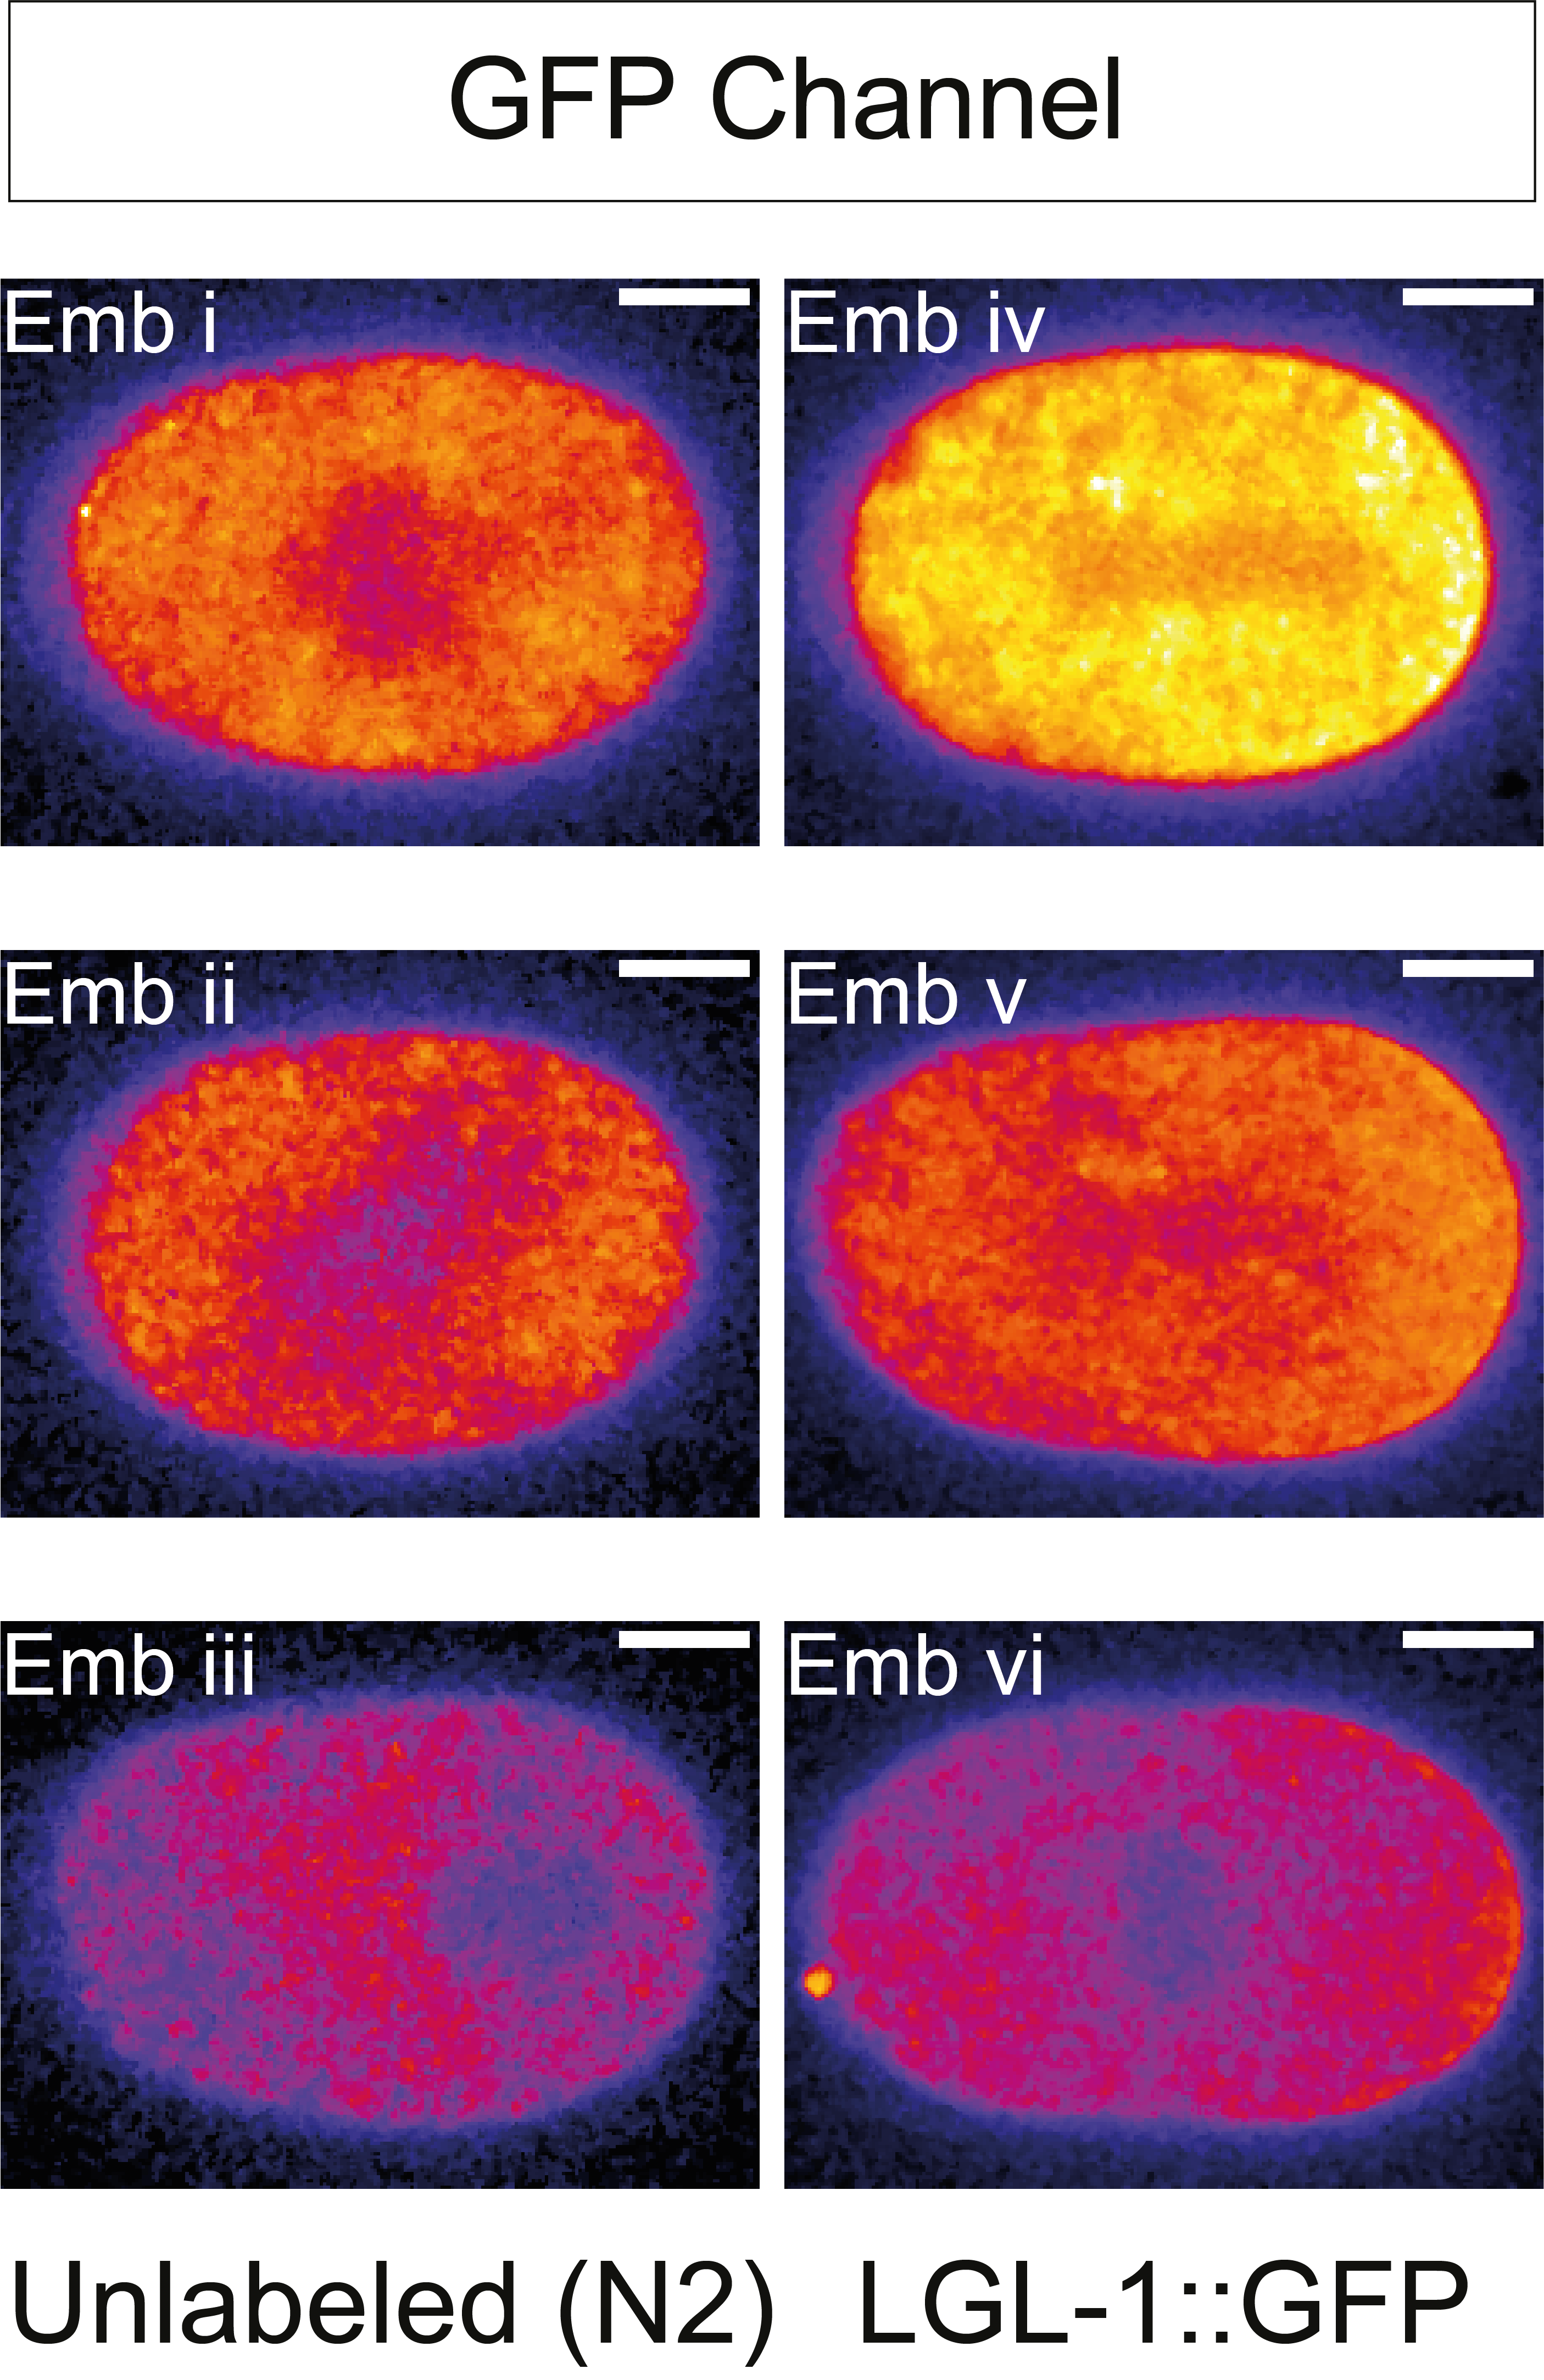
\includegraphics[scale=0.9]{saibr_n2_vs_lgl}
\mycaption{Autofluorescence is abundant and variable in images of \textit{C. elegans} zygotes}{GFP channel (488nm excitation, 535/50nm emission) images of unlabelled N2 and LGL-1::GFP embryos taken under identical imaging conditions. Pixel scaling is the same for each image. Figure panels from \textcite{Rodrigues2022}, Fig 1B.
}
\label{fig:saibr_n2_vs_lgl}
\end{SCfigure}

One approach that has been used to tackle autofluorescence in some systems is spectral imaging \citep{Billinton2001}. Typically used to separate overlapping fluorophore signals based on spectral characteristics, this approach can also be used to separate out autofluorescence by treating it much like a fluorophore with its own spectral characteristics. Whilst often effective, these techniques require specialised instruments and analysis tools, along with accurate prior knowledge of fluorophore spectra.\\

A simpler, related, approach has been proposed for some systems (e.g. \cite{Roederer1986}) which exploits the fact that autofluorescence can often be described as a single fluorescent component, with an emission spectrum much broader than GFP. If one can find an emission wavelength (usually red shifted) that is specific for autofluorescence, this can be used to infer the amount of autofluorescence in the sample, which can then be subtracted away from the regular fluorophore channel to give a clean readout of fluorophore signal. In comparison to full spectral imaging, this method can be carried out with standard light sources and emission filters, and therefore can be easily implemented in existing workflows.\\

Inspired by this approach, we aimed to implement, and assess the applicability of such a method for autofluorescence removal in images of \textit{C. elegans} embryos. In doing so, we have put together a robust and easily-implementable workflow which we have termed SAIBR: Spectral Autofluorescence Image correction by Regression.\\


\subsection{SAIBR: a simplified method for autofluorescence correction based on dual emission imaging}


At minimum, autofluorescence correction relies on the ability to find a reporter channel that is free of GFP signal, but rich in autofluorescence, such that this channel can be used as an independent readout of autofluorescence in the sample. Full spectral analysis performed by Nelio Rodrigues (not shown here), shows that a channel with a red shifted emission filter, such as those commonly used to image red fluorescent proteins, meets such a requirement.\\

Furthermore, by imaging untagged embryos with both the standard GFP channel and this red-shifted autofluorescence-reporter channel (488nm excitation, 630/75nm emission), which I will refer to as the AF channel, we find a strong linear correlation between pixel data from the two channels (\cref{fig:saibr_n2_correlation}). Whilst raw pixel values do not correlate well, as these are dominated by noise, we can get a strong correlation by first applying a Gaussian filter to suppress this noise (\cref{fig:saibr_n2_correlation}A). We found that this relationship is consistent between embryos (\cref{fig:saibr_n2_correlation}B, C). Furthermore, we found a near identical relationship when plotting the mean intensity values of individual embryos, suggesting that the same relationship can account for both intra- and inter-embryo AF variation. \\

\begin{figure}
\includegraphics[scale=0.95]{saibr_n2_correlation}
\centering
\mycaption{Autofluorescence is spatially correlated across emission channels}{
\textbf{(A)} Correlation of pixel values between the GFP channel and AF channel for an unlabelled N2 embryo, subject to Gaussian blur of indicated radius. Pixel values were taken from a region of interest (ROI) encompassing the entire embryo and a portion of the background. All pixels within this region were used for the regression, but for clarity only a random 10\% sample of pixels are shown.
\textbf{(B)} Comparison of inter-channel pixel correlation (Gaussian radius = 1) for three unlabelled N2 embryos, colour coded by embryo. Histograms of intensity values for GFP and AF channels shown for reference.
\textbf{(C)} Comparison of per-pixel correlation with data obtained from whole embryo means. (i) Lines indicate per-pixel regression for individual embryos as in (B). (ii) Overlay showing mean whole embryo fluorescence values (circles).
Figure panels from \textcite{Rodrigues2022}, Fig S2, 1E-F.
}
\label{fig:saibr_n2_correlation}
\end{figure}

Together, this implies that taking an AF channel image should be sufficient to accurately predict the level of autofluorescence in the GFP channel, and thus subtract it out. To quantify the necessary inter-channel conversion factors, I performed linear regression, using an ordinary least squares method, on Gaussian-filtered pixel values pooled from multiple untagged embryos. Then, to perform correction on images containing fluorophore, we just need to capture an AF channel image, alongside the GFP channel image, rescale the AF image according to the predefined conversion factors, and then subtract this inferred autofluorescence away from the GFP channel image pixel-by-pixel.\\


\subsection{Assessing SAIBR performance on images of PAR proteins}

To assess the effectiveness of SAIBR, and its utility in the analysis of PAR proteins, I applied it to a range of images of unlabelled and GFP-labelled embryos. As expected, applying SAIBR to images of unlabelled cells reduced fluorescence from across the cells to zero, with no visible structures remaining (\cref{fig:saibr_spatial_correction}A). This suggests that the method can fully account for all autofluorescence in the cell.\\

In the case of LGL-1::GFP expressing embryos, where autofluorescence signal is dominant (\cref{fig:saibr_n2_vs_lgl}), SAIBR removes autofluorescence signal within the cell, and improves contrast at the posterior cortex, allowing us to better resolve plasma membrane enrichment \cref{fig:saibr_spatial_correction}B. Improvements are just as striking for PAR-3::GFP. In addition to improvements at the cortex, we see that SAIBR can suppress the local fluorescence minimum at the cell centre caused by lower AF at the pronuclei. For PAR-6::GFP the improvements are qualitatively less striking, as the ratio of fluorophore signal to autofluorescence is higher, but nonetheless AF removal has a quantitative impact.\\

\begin{figure}
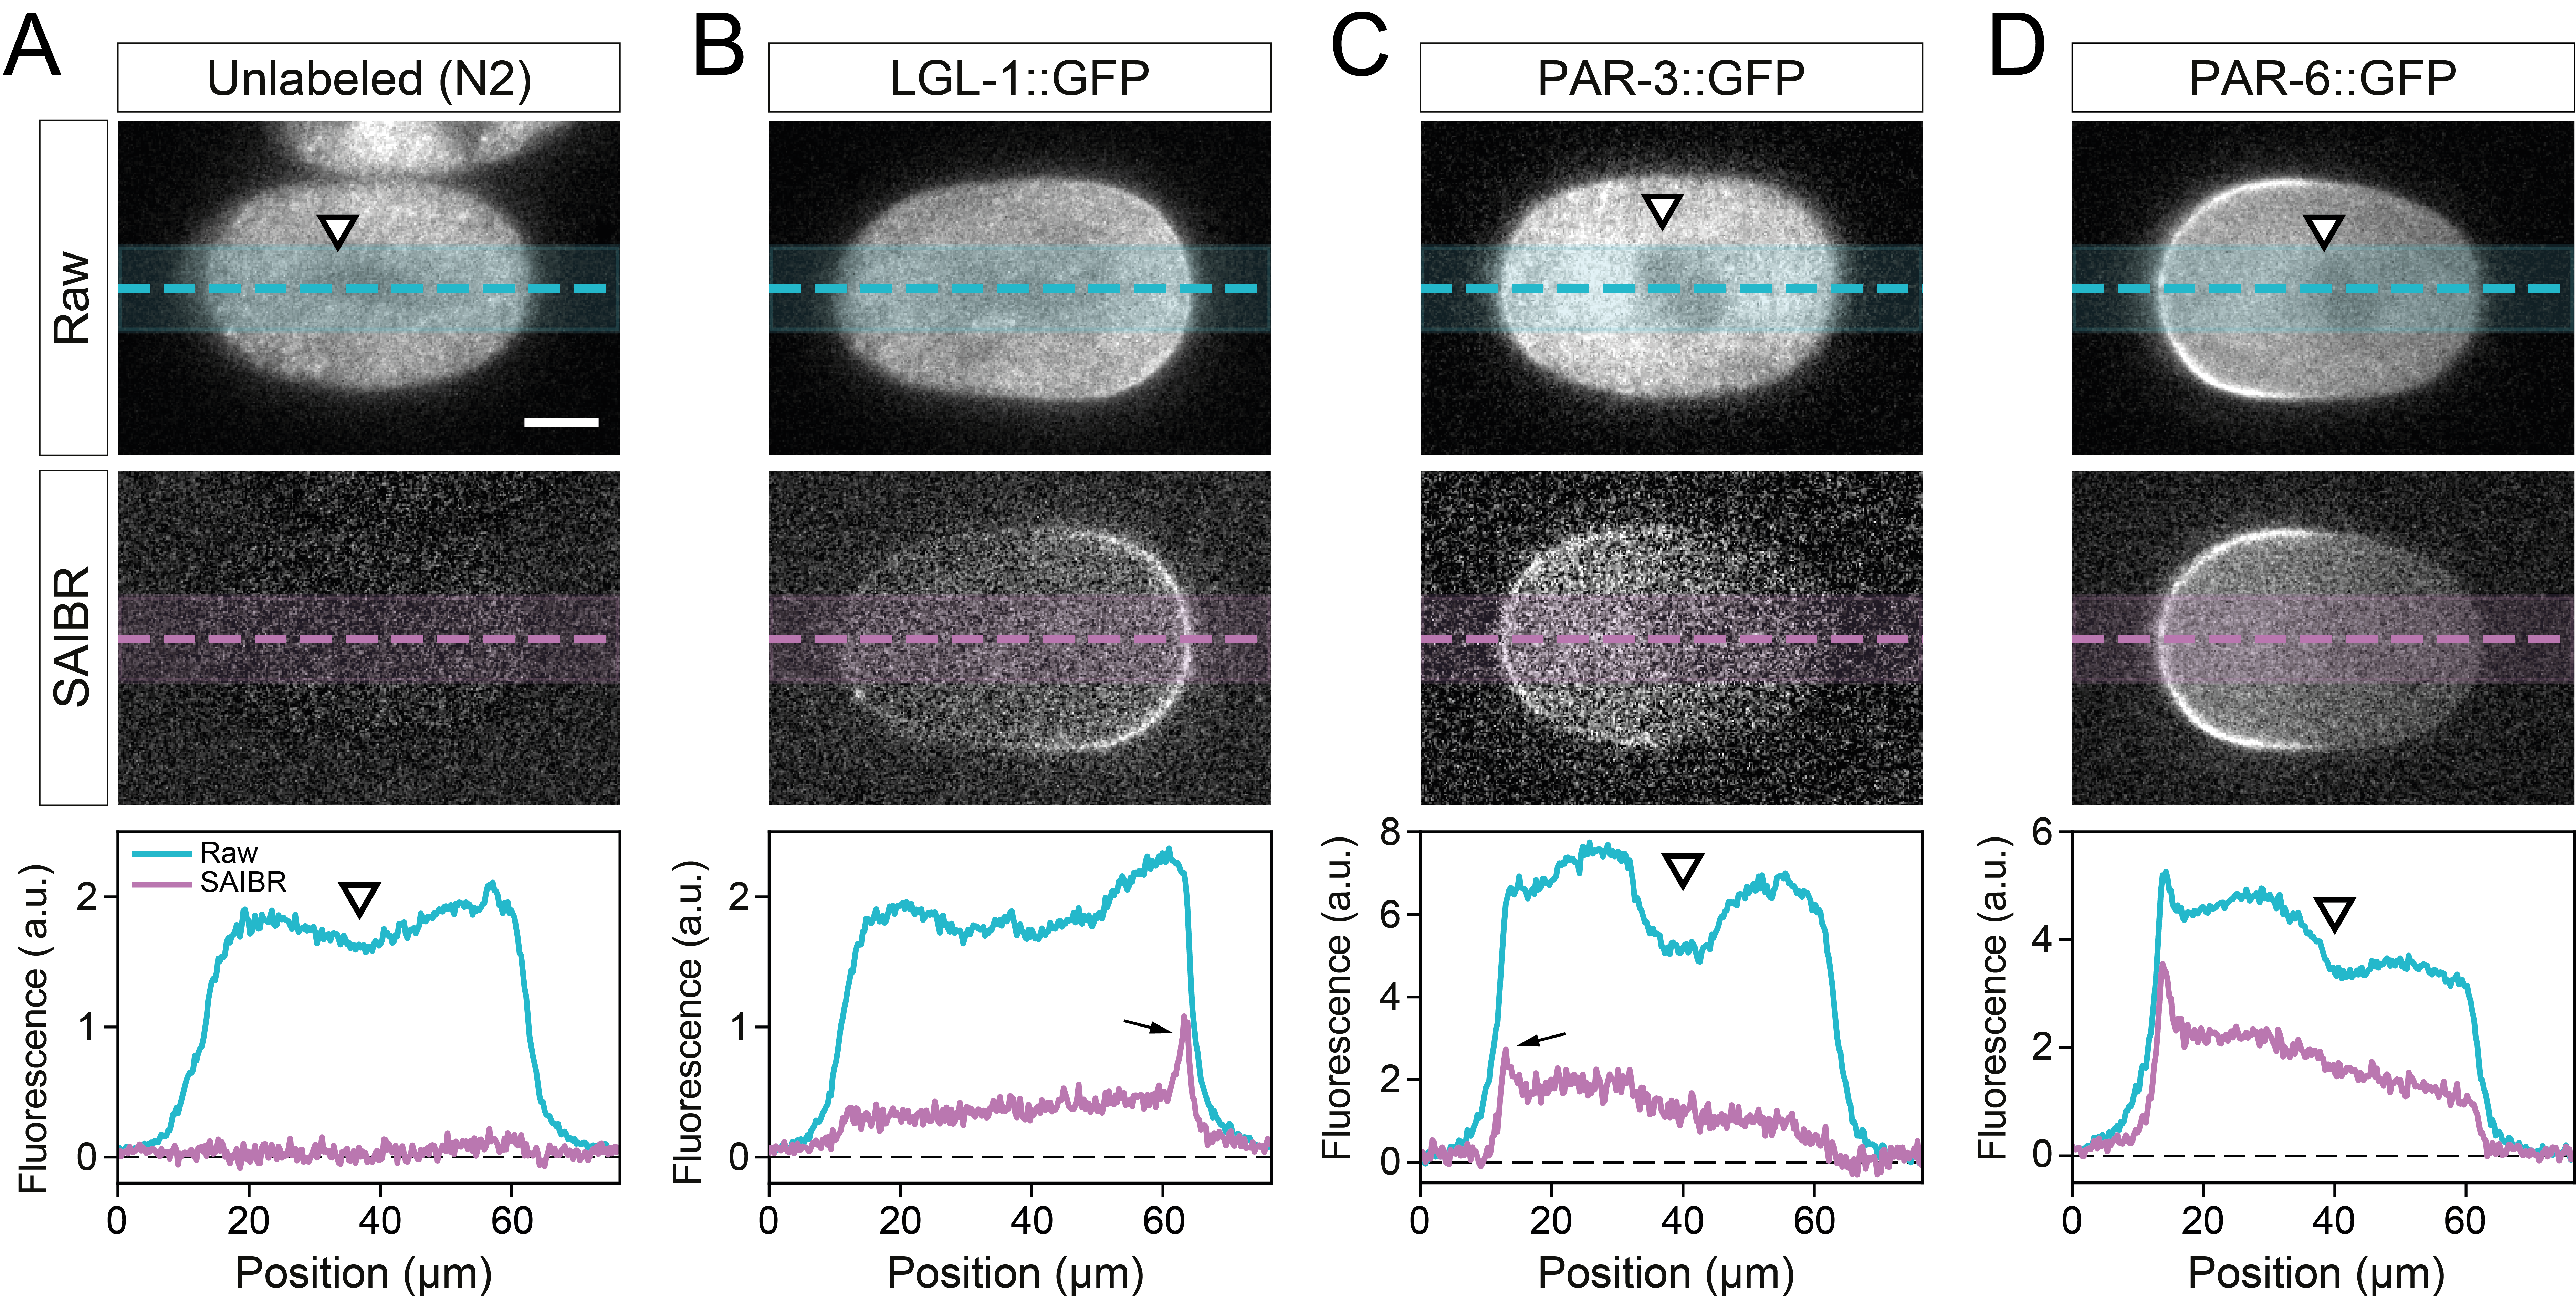
\includegraphics[scale=0.9]{saibr_spatial_correction}
\centering
\mycaption{Applying SAIBR to images of GFP-tagged PAR proteins}{
\textbf{(A) - (D)} Raw (top) and SAIBR-corrected (middle) midplane images of zygotes expressing the indicated GFP fusions. Bottom panels show associated linescans across the images. SAIBR reveals prominent membrane localisation for LGL-1 and PAR-3 (arrows) which is not obvious in uncorrected images. We also see a prominent signal dip in the pronuclear region of uncorrected images due to local exclusion of autofluorescence (arrowheads), which disappears in SAIBR corrected images.
Figure panels from \textcite{Rodrigues2022}, Fig 2A-D.
}
\label{fig:saibr_spatial_correction}
\end{figure}

As shown in \cref{fig:saibr_membrane_profiles}, SAIBR has a strong impact on the shape of intensity profiles taken across the cortex within each polarity domain, in all cases showing a clearer peak and suppression of signal at the internal portion of the curves. This has particular importance for quantitative studies because, as described in section \ref{section:memquant}, the shape of cross-cortex profiles are often used to quantitatively analyse membrane concentrations and/or membrane affinities. For example, a cross-cortex profile with a central peak that is much higher than the internal cytoplasmic plateau clearly implies that the protein is binding to the membrane with a high affinity. We can see from the SAIBR corrected profiles that, of the three proteins shown here, LGL-1 has the strongest membrane affinity (highest enrichment at the membrane compared to its cytoplasmic level), followed by PAR-6, followed by PAR-3. If we look at the profiles pre-correction, however, this is not so clearly apparent. One might have had some success by simply subtracting an equivalent average profile taken from untagged N2s, but such a method would fail to account for the fact that much of variation between embryos is down to autofluorescence, and would therefore be unsuitable for studies where inter-embryo variation is important. In the case of LGL-1 this would also clearly result in negative values at the cytoplasmic portion of the curve for some embryos.\\

\begin{figure}
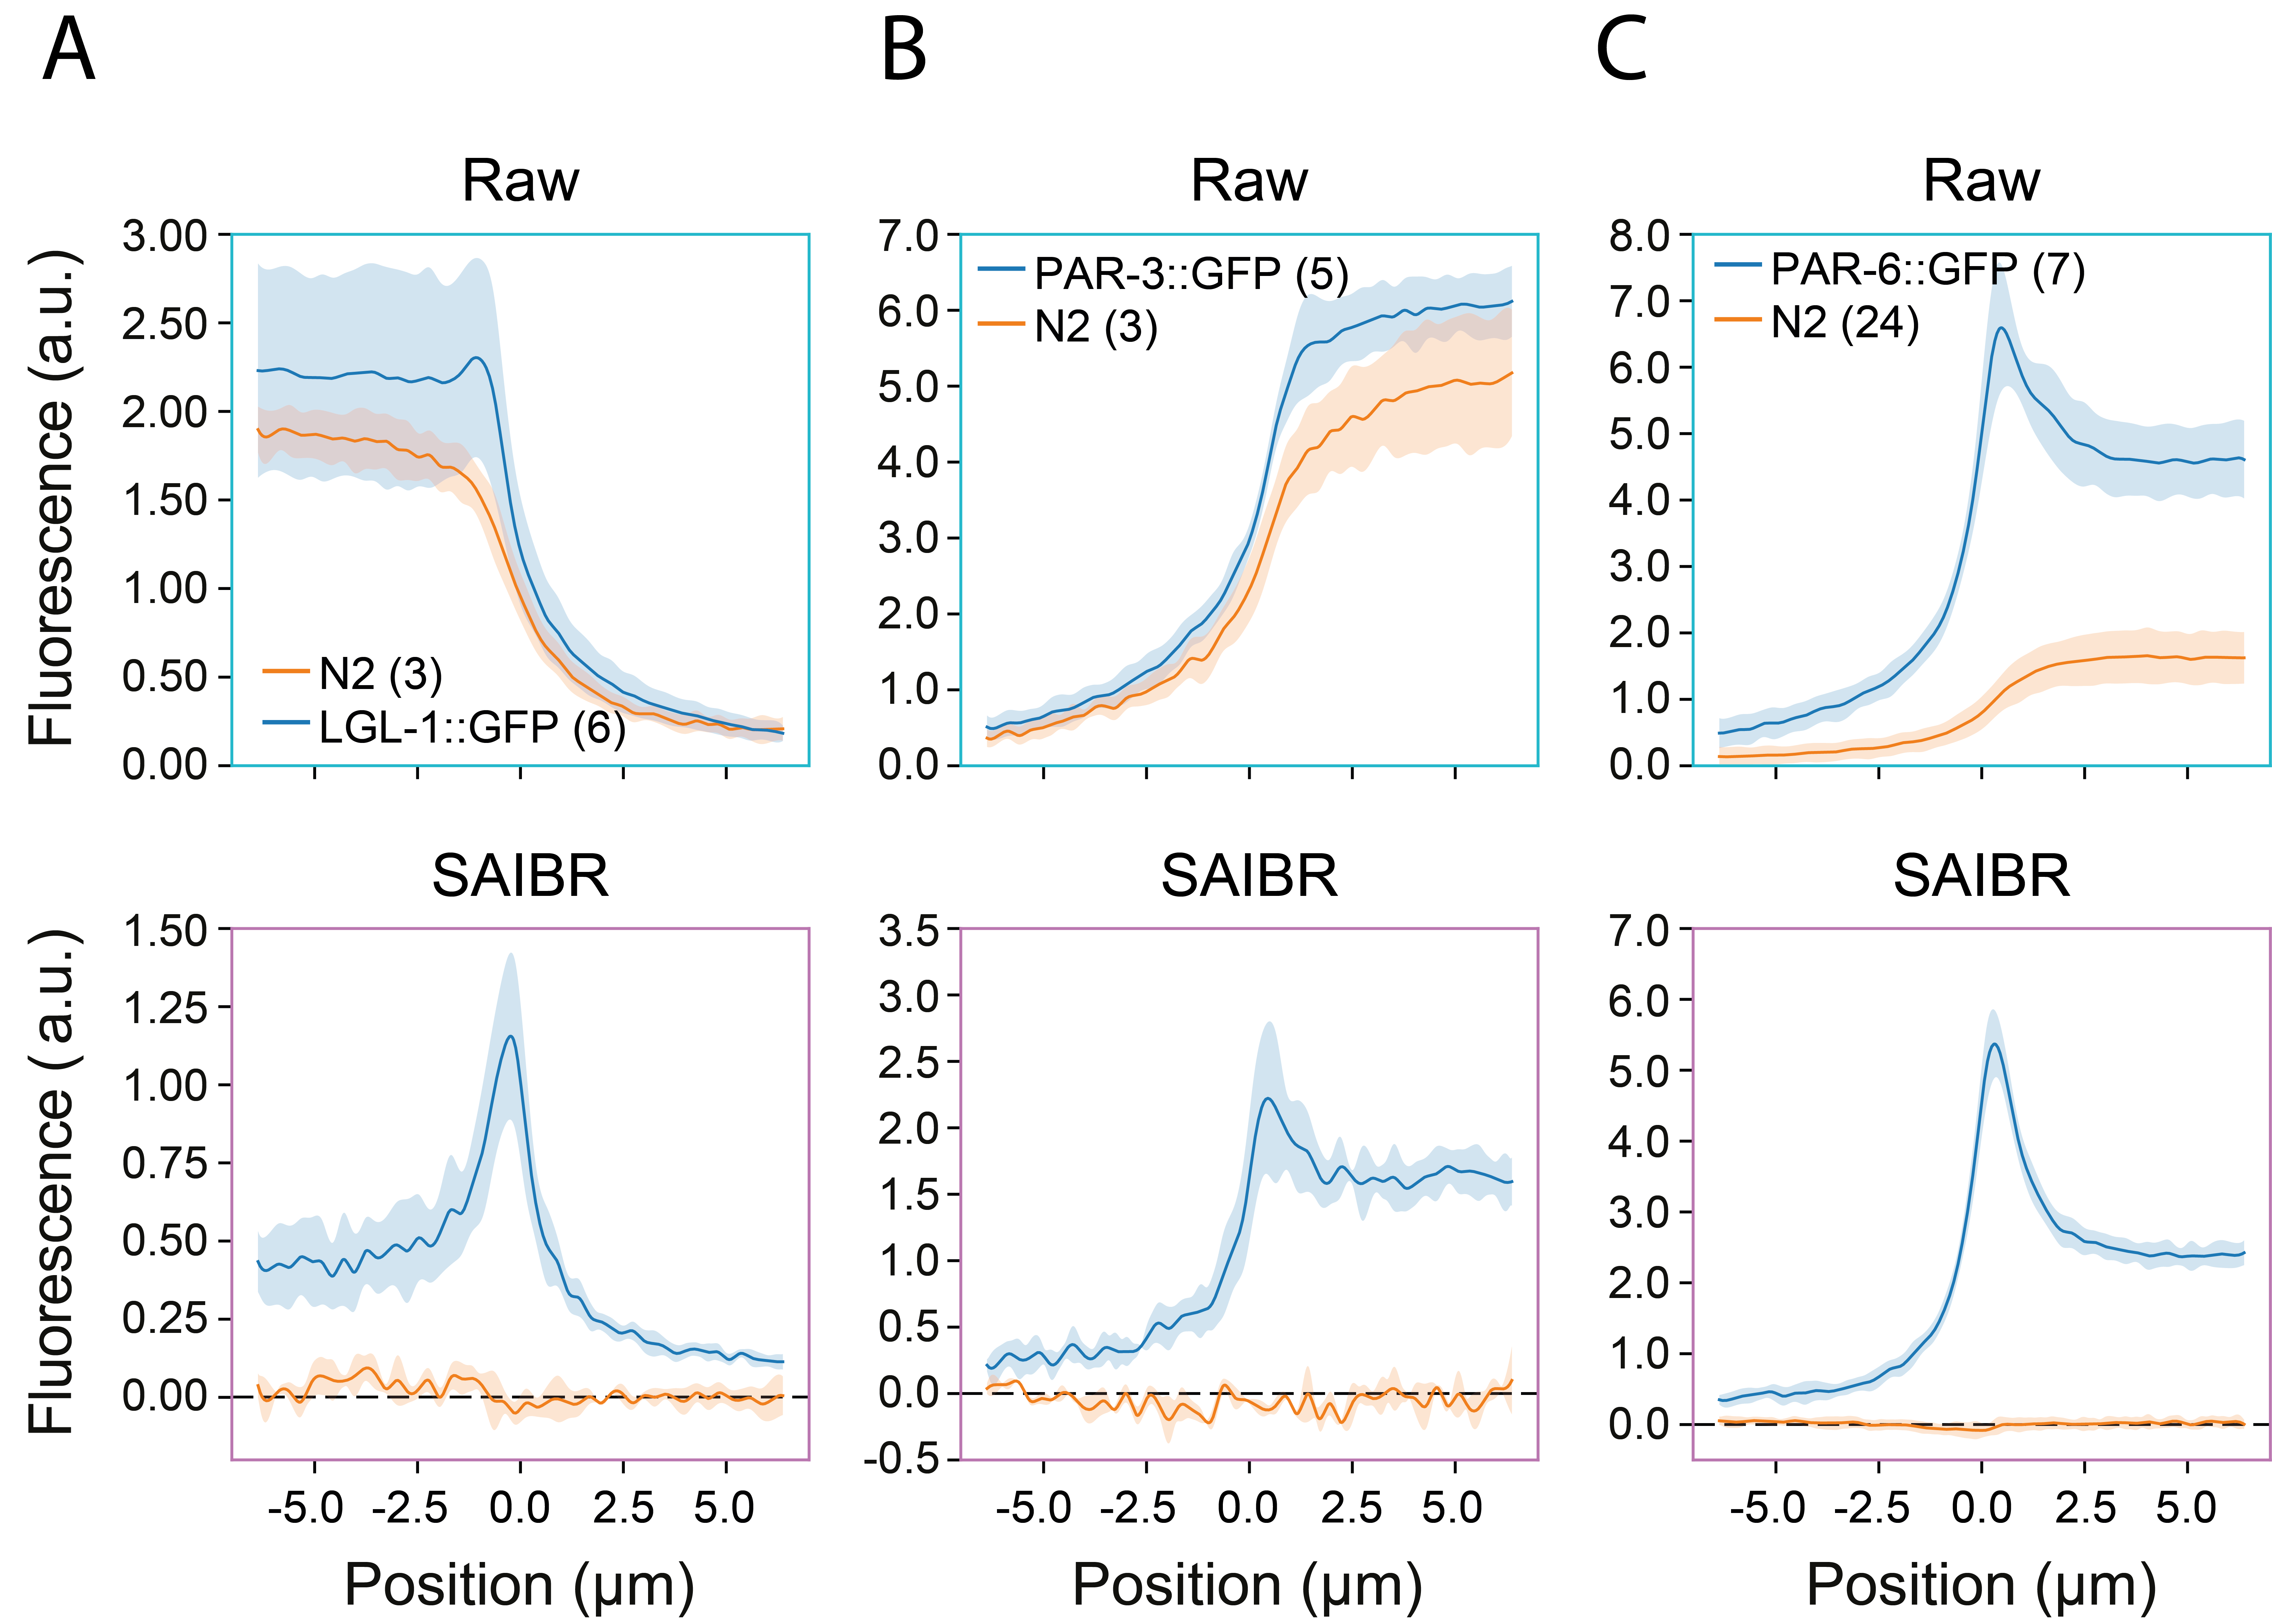
\includegraphics[scale=1]{saibr_membrane_profiles}
\centering
\mycaption{SAIBR improves detection of membrane signals}{
\textbf{(A) - (C)} Averaged membrane profiles taken from raw (top) and SAIBR-corrected (bottom) images for LGL-1::GFP (A), PAR-3::GFP(B) and PAR-6::GFP (C) shown relative to unlabelled N2 controls. Membrane position at x=0$\mu m$. Mean $\pm$ SD indicated.
Figure panels from \textcite{Rodrigues2022}, Fig. 2E-G.
}
\label{fig:saibr_membrane_profiles}
\end{figure}

\subsection{Extending SAIBR to dual-labelled \textit{C. elegans} embryos}

As SAIBR relies on a red shifted emission channel, complications can arise in samples containing red fluorophore. As red fluorophores are usually weakly excited by blue lasers, they will contribute additional signal to the AF channel, which may lead to overestimation, and therefore oversubtraction, of autofluorescence if not accounted for. If RFP levels are low, this effect may be small and can be ignored. However, if RFP levels are high, this bleedthrough effect can be significant. This can be demonstrated by observing the inter-channel relationship in control embryos expressing mCh::MEX-5 (\cref{fig:saibr_3channel_correlation}A). We find that, when an RFP is present, this relationship deviates significantly from the typical relationship observed in N2s, in direct proportion to local signal in the RFP (561nm excitation, 630/75nm emission) channel (\cref{fig:saibr_3channel_correlation}A inset). As this relationship is linear, autofluorescence in the GFP channel can be described as a linear function of both the AF and the RFP channels. Plotting pixel data in three dimensions shows that the data can be successfully fit to a plane, by performing multiple linear regression (\cref{fig:saibr_3channel_correlation}B, C). \\


\begin{figure}
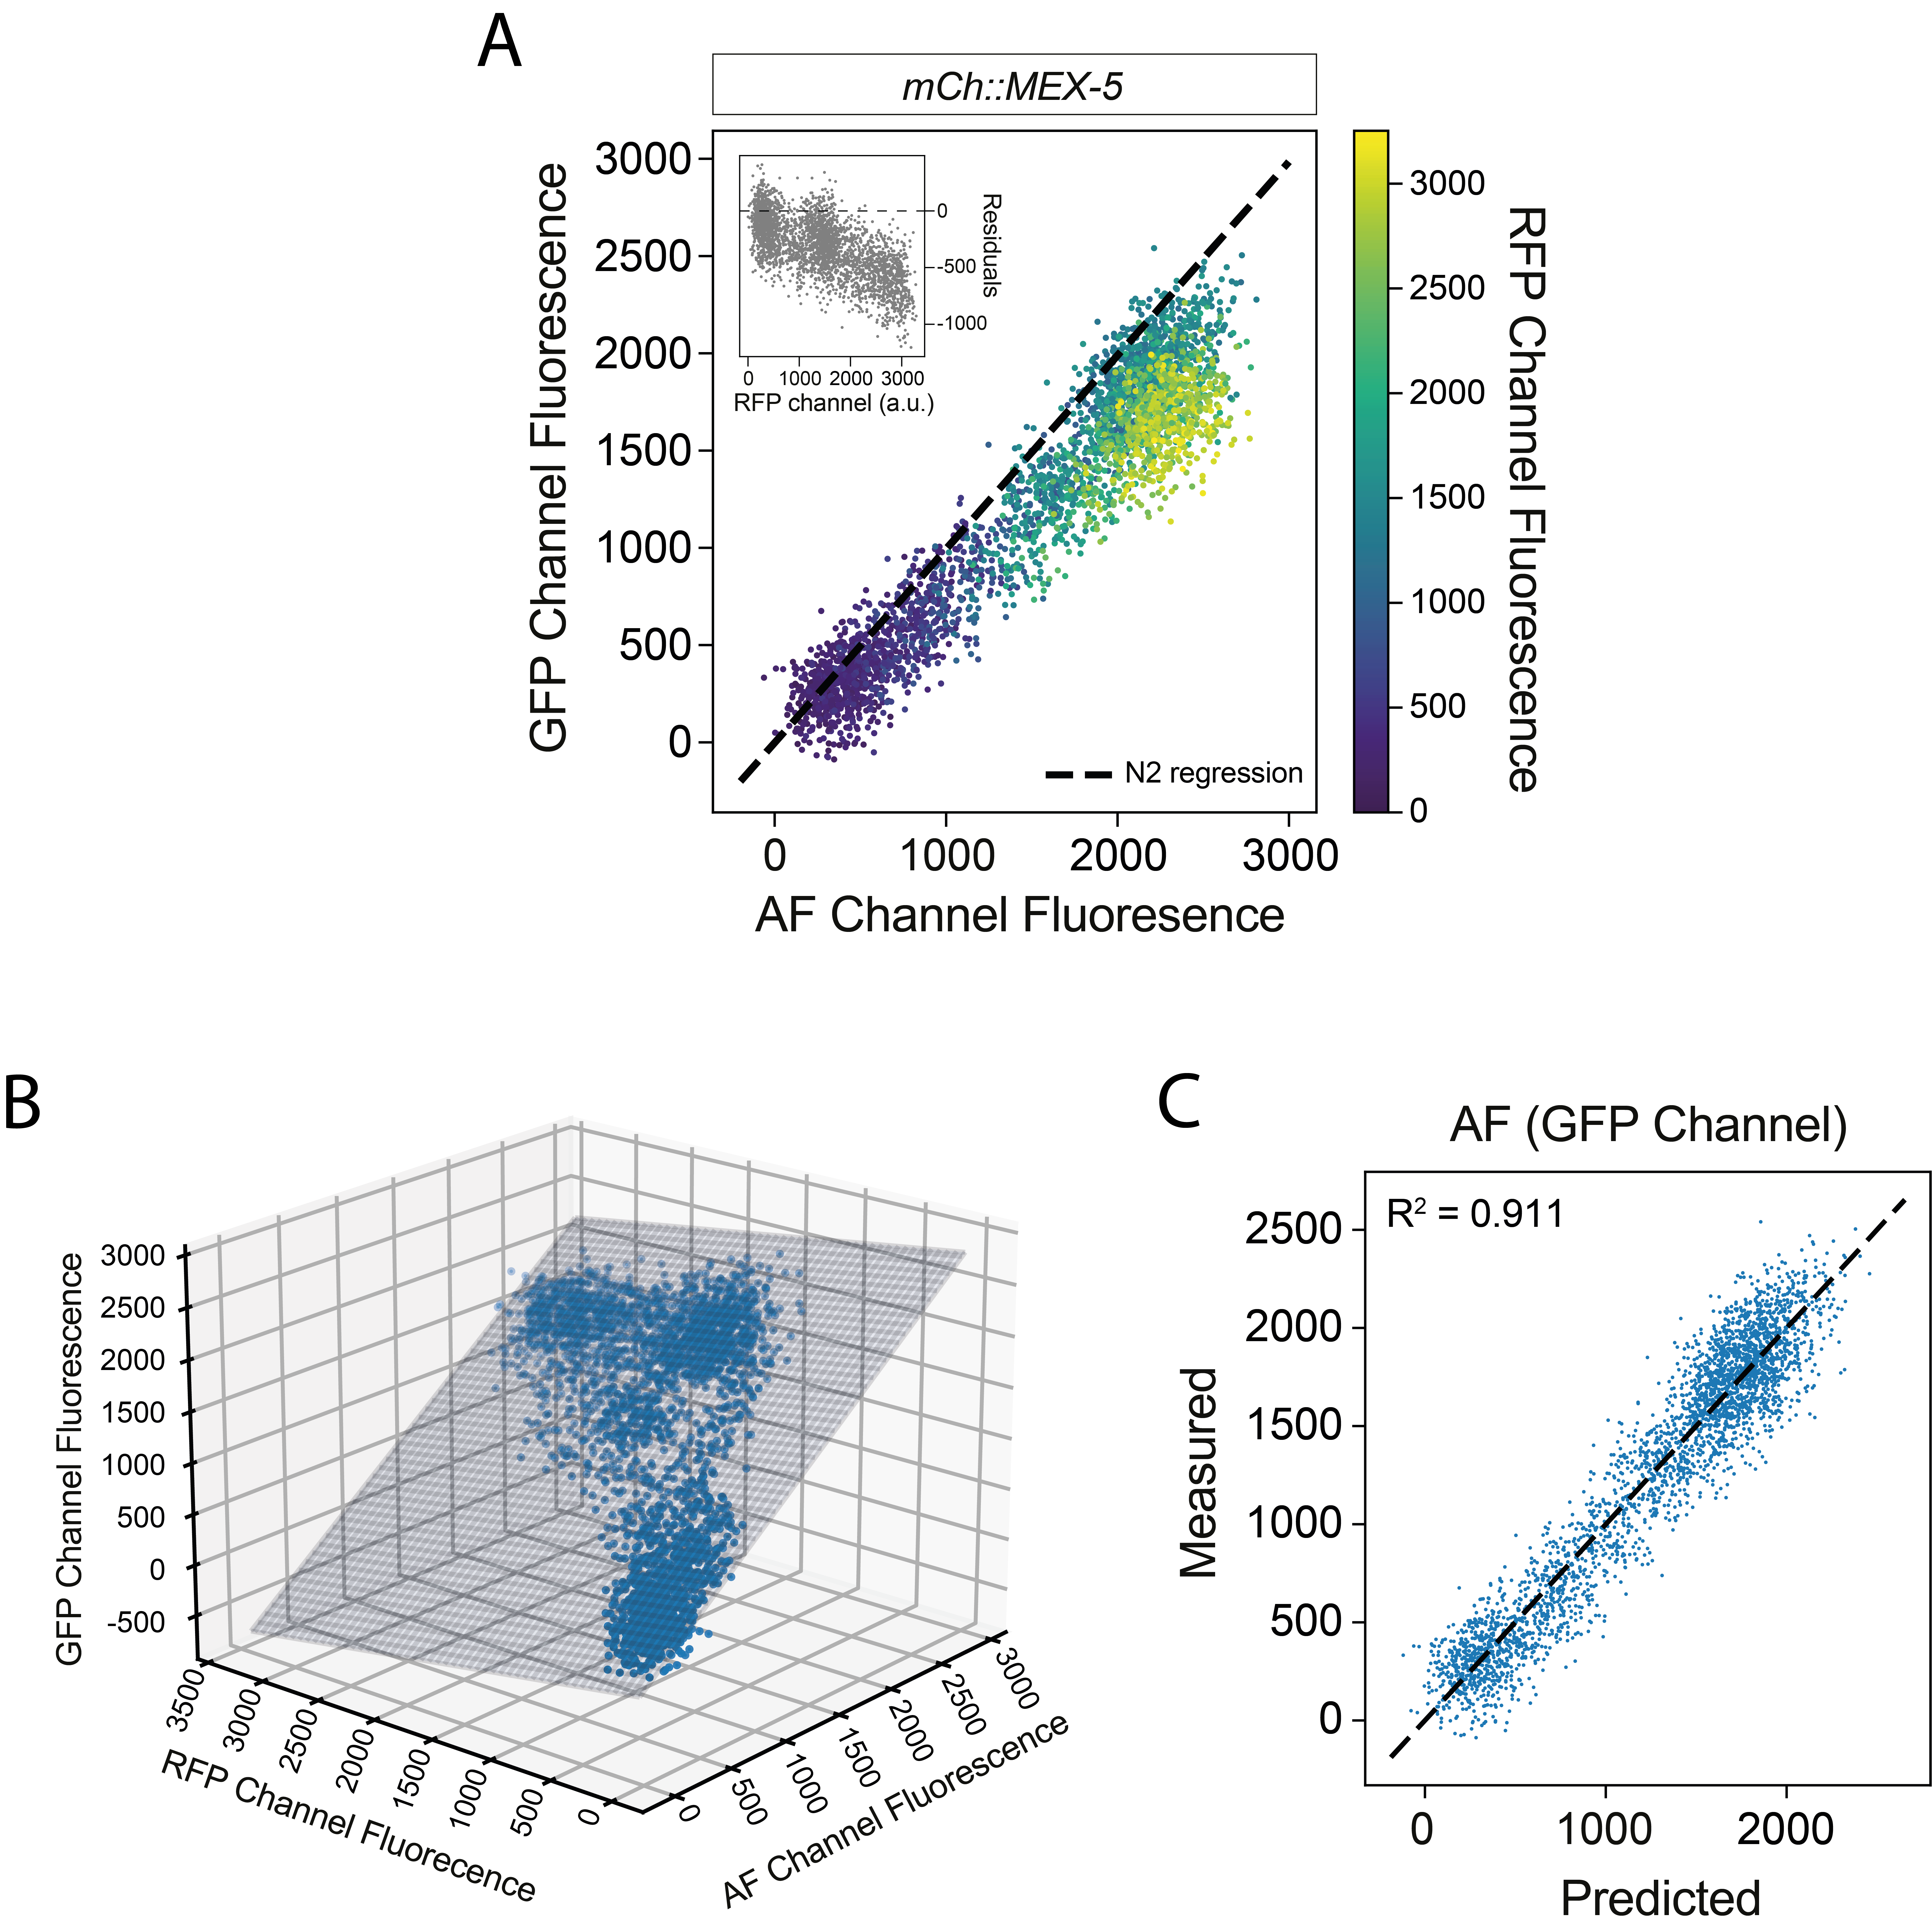
\includegraphics[scale=1]{saibr_3channel_correlation}
\centering
\mycaption{Pixel intensities correlate across three channels in samples containing red fluorophore.}{
\textbf{(A)} Gaussian-filtered (radius = 1) GFP channel vs AF channel pixel intensities for an mCh::MEX-5 expressing embryo, colour coded by RFP-channel fluorescence. Dashed line indicates the AF vs GFP correlation for untagged (N2) embryos. Inset shows residuals as a function of RFP channel signal. Pixels taken from an ROI encompassing the embryo and a region of the background, and 10\% of pixels are shown at random.
\textbf{(B)} Multiple regression fit of GFP-channel signal as a function of AF and RFP channel signal. The same embryo and sample of pixels as in (A) is shown.
\textbf{(C)} Predicted vs. measured GFP-channel signal based on the fit in (B). The same embryo and sample of pixels as in (A) and (B) is shown.
Figure panels from \textcite{Rodrigues2022}, Fig. 4B-D.
}
\label{fig:saibr_3channel_correlation}
\end{figure}

To perform correction on images containing red fluorophore, we just need to capture all three channels, calculate autofluorescence using the three-channel regression relationship obtained from the appropriate RFP-tagged single line, and then subtract this away from the GFP channel image. This is demonstrated in \cref{fig:saibr_3channel_correction}, for embryos expressing both PAR-6::GFP and mCh::MEX-5, or just mCh::MEX-5. Whereas 2-channel SAIBR results in oversubtraction of autofluorescence (particularly visible in the mCh::MEX-5 single line), this is eliminated when using 3-channel SAIBR.\\

\begin{SCfigure}
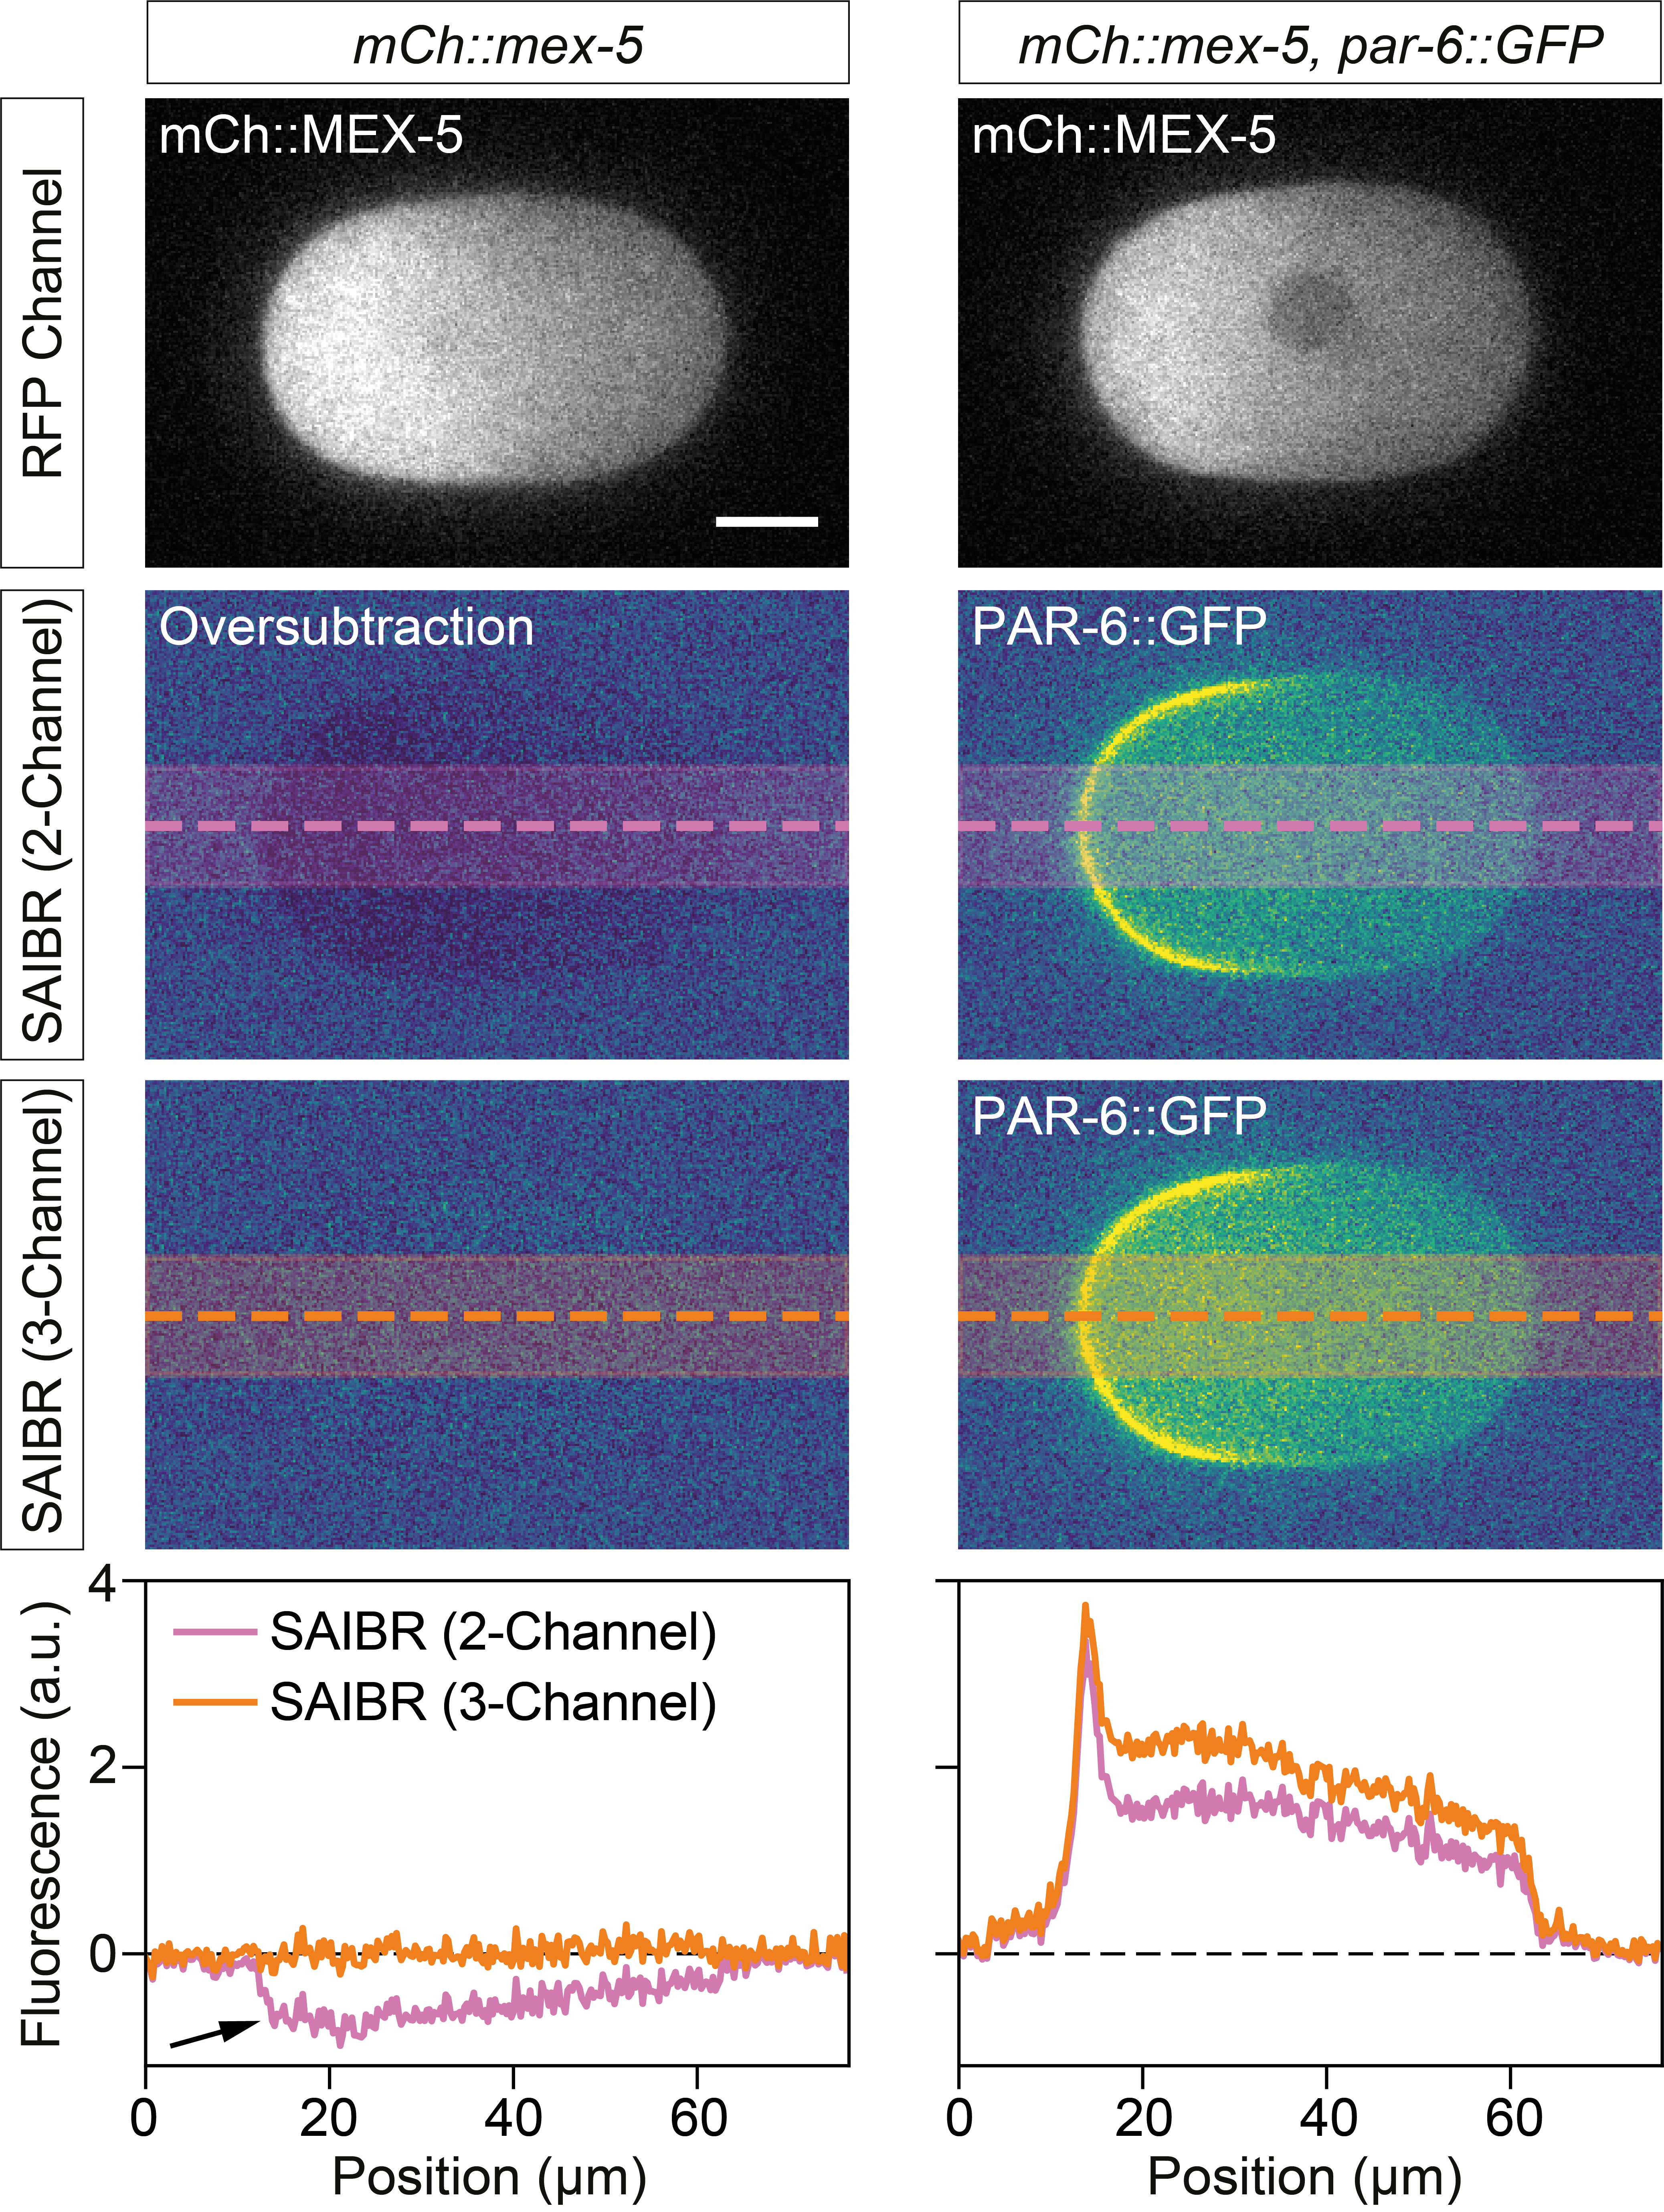
\includegraphics[scale=1]{saibr_3channel_correction}
\mycaption{3-channel SAIBR prevents oversubtraction in samples containing red fluorophore}{
RFP channel, 2-channel SAIBR and 3-channel SAIBR images for samples expressing mCh::MEX-5, along with associated linescans. 2-channel SAIBR results in oversubtraction which is clearly visible as negative values in the mCh::MEX-5 line (arrow) and reduced cytoplasmic signal in the two-colour line. 3-channel SAIBR, using the calibration procedure shown in \cref{fig:saibr_3channel_correlation}, prevents oversubtraction.
Figure panels from \textcite{Rodrigues2022}, Fig. 4F.
}
\label{fig:saibr_3channel_correction}
\end{SCfigure}


\subsection{Discussion}

In summary, I have demonstrated that a simple protocol, which we have termed SAIBR, can be used to successfully remove autofluorescence in images of \textit{C. elegans} zygotes. The improvements are particularly striking for images of fusion proteins with low levels of expression, such as LGL-1::GFP, but even in cases where expression levels are higher, AF correction will prove important for quantitative analysis of membrane concentrations, as will be discussed in the next section. For the rest of this thesis, unless otherwise stated, green fluorophore images will be presented with autofluorescence removed by SAIBR.\\

The simplicity of the method means that it can be easily incorporated into existing workflows, and should be applicable to a variety of imaging platforms. In the full study \citep{Rodrigues2022}, we show that the method is equally successful on both spinning-disk confocal and wide-field instruments. \\

Whilst initially developed with \textit{C. elegans} embryos in mind, the method is not specific to this system, and could be applied to a number of other model systems in which autofluorescence is a problem. In the full study, we show that the method works successfully in \textit{C. elegans} larvae, as well as other model systems such as starfish oocytes and fission yeast (\textit{S. pombe}). That said, the method is not guaranteed to perform well in all cases. If samples contain multiple, independently varying sources of autoflourescence, then SAIBR may face problems as a single autofluorescence reporter channel cannot account for this. However, much like how we can tackle red fluorophores, we have found that in some cases this can be solved simply by adding one extra reporter channel. Inevitably, though, such an approach may not be compatible with dual-colour imaging. \\

Whilst the analysis steps are relatively straightforward, implementing the computational workflow may still be a barrier to adoption for some. Therefore, to make the protocol accessible, I have put together a simple graphical user interface (GUI)-based FIJI plugin which can carry out all the necessary analysis in a few simple steps. This can be found at: \url{https://github.com/tsmbland/saibr_fiji_plugin}. \\

The method comes with a few tradeoffs, which will vary in significance depending on the particular study. One issue is that, as the method combines pixel noise from multiple images, corrected images can in some cases be quite noisy, particularly where weak imaging conditions are used. It also requires capturing two emission channels for each image, which doubles sample illumination times and potential phototoxicity, which may be an issue for long timelapses. Additionally, if samples display rapid motion, then the time lag between taking these two channels may lead to pixel mismatches, which could introduce artefacts. These last points could be fixed by using an imaging setup that allows for dual capture of multiple emission bands. However, for this particular study, these issues will not be of major significance. \\


\clearpage
\section{Extracting membrane and cytoplasmic signal components}
\label{section:memquant}

% Transition

\subsection{An overview of existing methods}

A number of methods have been implemented aiming to quantify protein concentrations at the membrane and in the cytoplasm in images of \textit{C. elegans} embryos. A typical approach to quantify membrane concentrations is to find the region of the image representing the cortex (either by manual or computational segmentation) and take a coarse measure of pixel values within this region (\cref{fig:memquant_method_comparison}, \textit{Intensity based quantification}). Such an approach was used by \textcite{Goehring2011a}, who manually segmented the embryo cortex in confocal images, computationally straightened a region around the circumference of the cell, and defined membrane concentrations as the sum of the highest intensity group of pixels at each cortical cross section. \textcite{Hubatsch2019a} used a similar approach, but replaced manual segmentation with an automated computational pipeline. Similarly, \textcite{Zhang2017} developed a computational protocol to segment images, and defined membrane concentrations around the cell as the average signal intensity within a region representing the cell cortex.\\

\begin{figure}
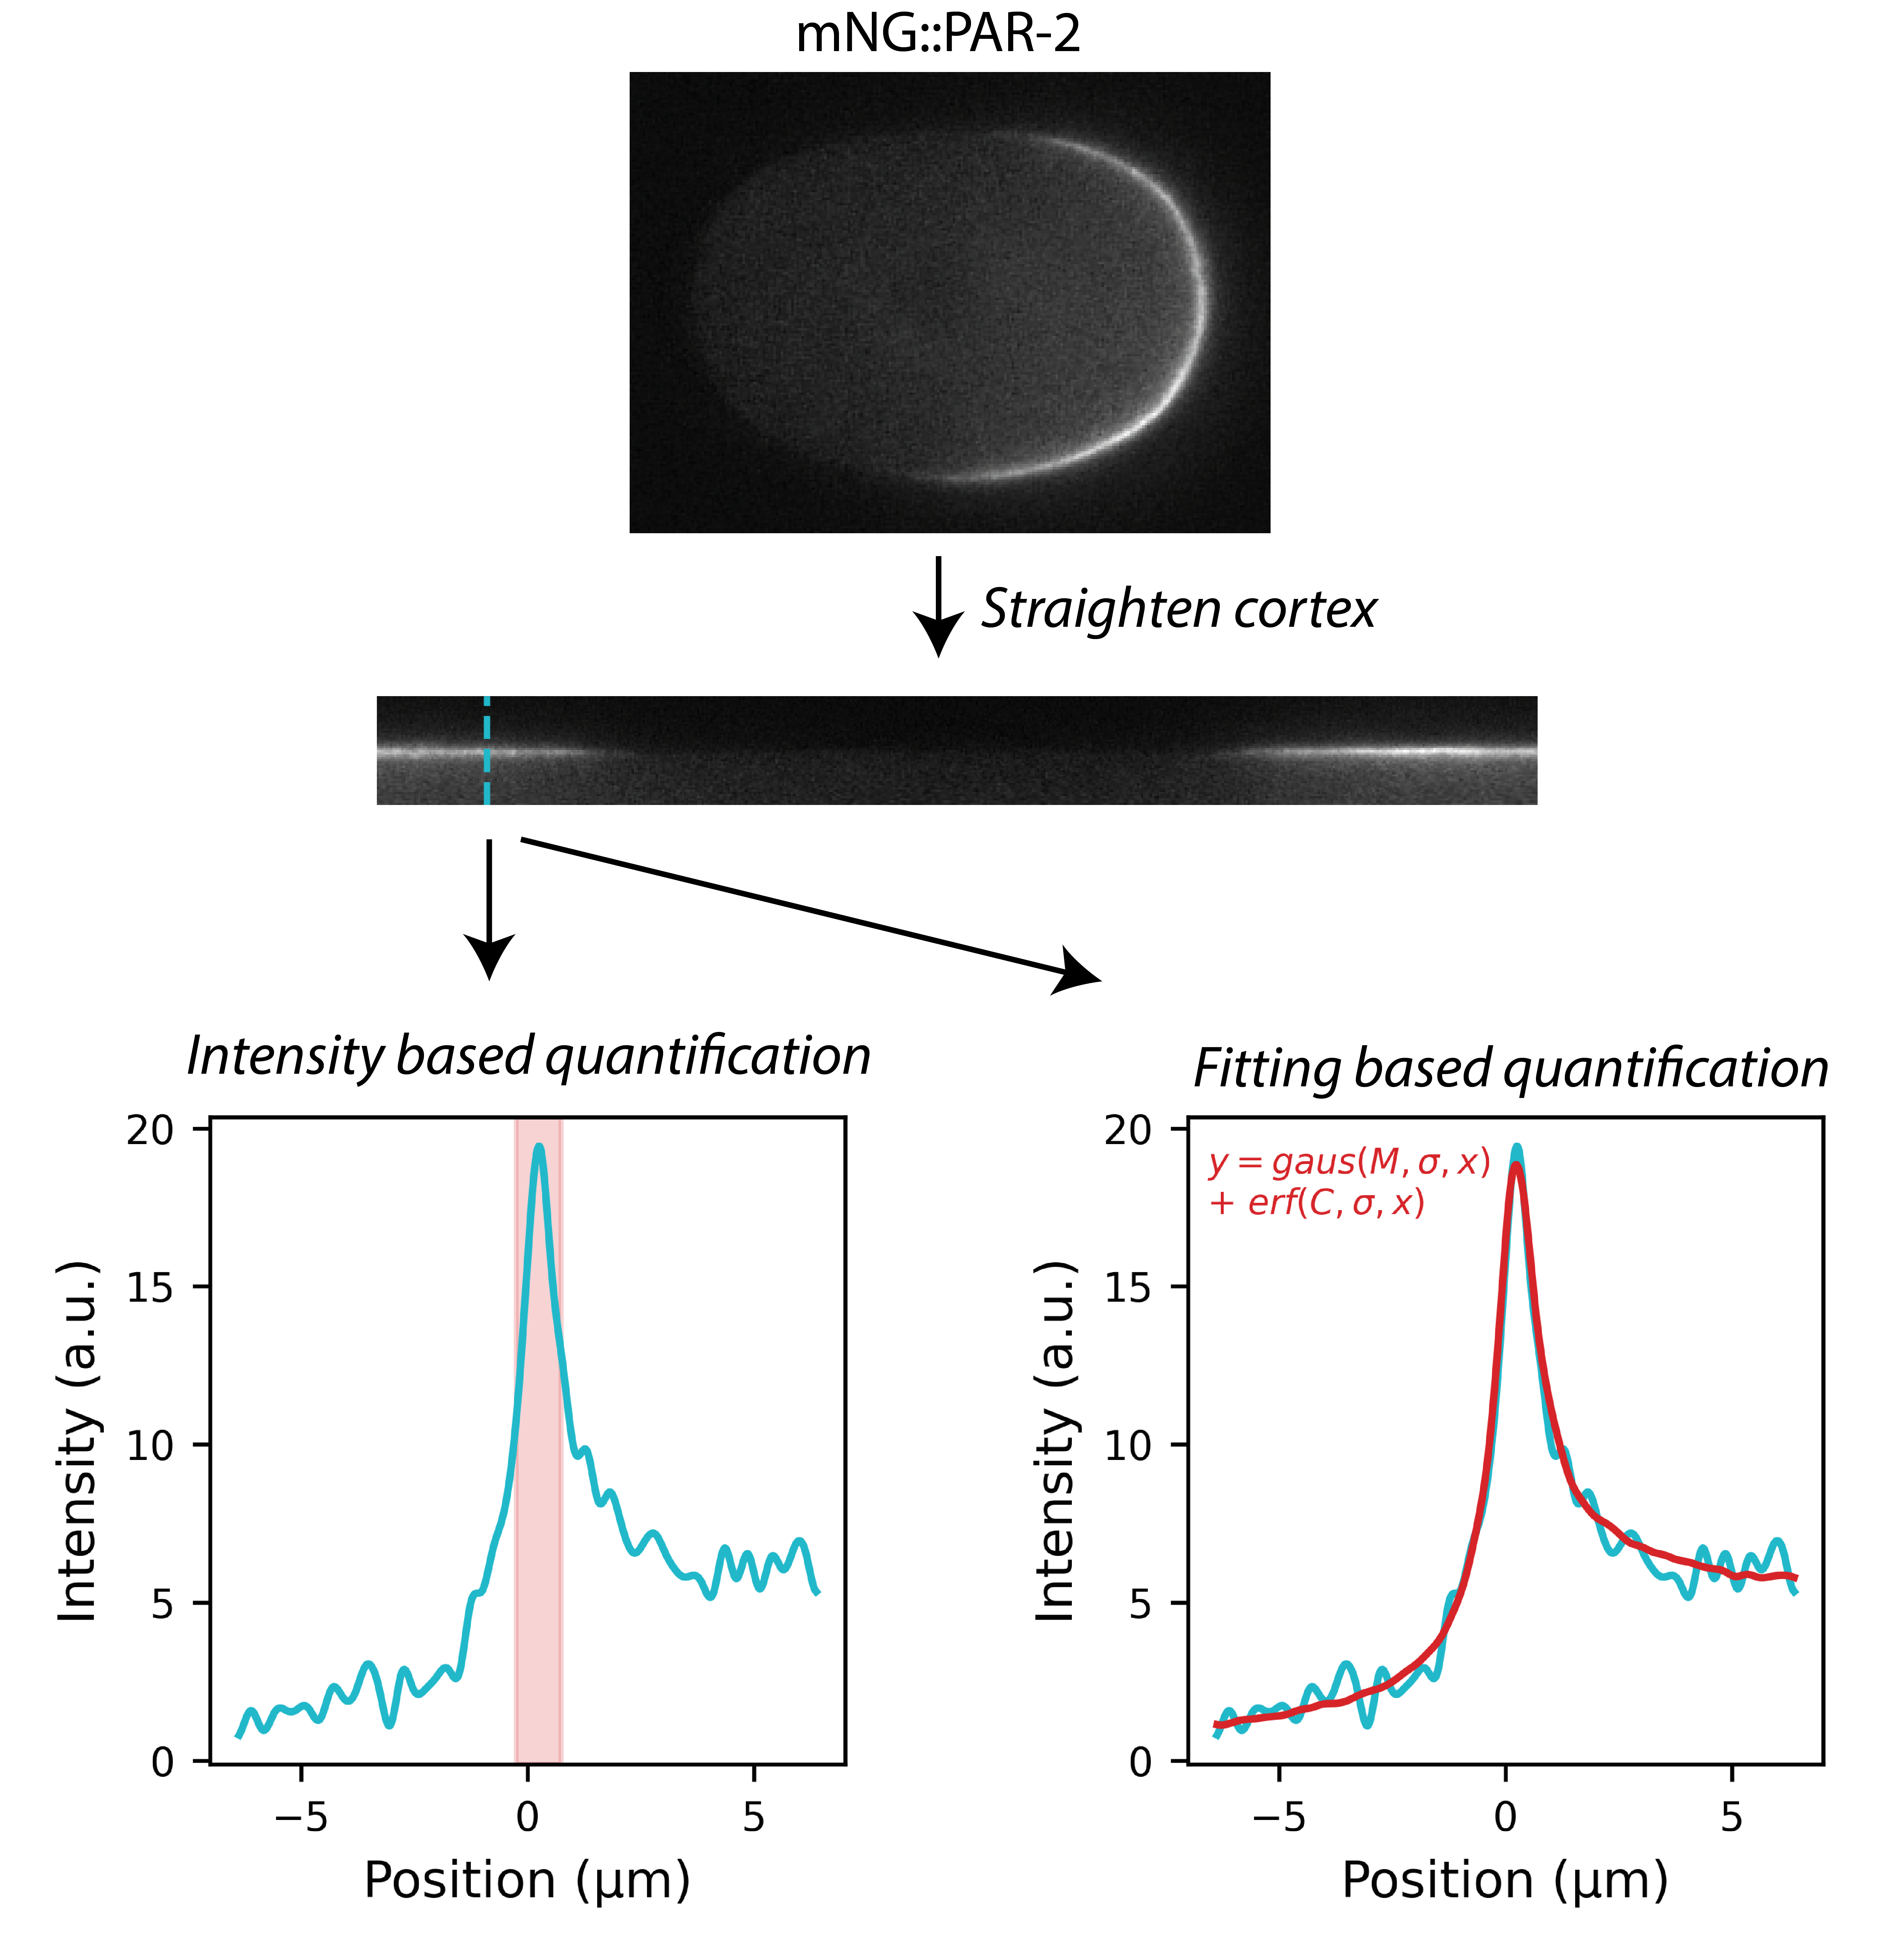
\includegraphics[scale=1]{memquant_method_comparison}
\centering
\mycaption{Approaches for quantifying membrane concentrations from midplane images}{Typical methods involve segmentation of embryos, either manually or computationally, followed by computational straightening, to simplify geometry, here shown for an image of mNG::PAR-2. Each position along the x-dimension of the straightened image represents a profile perpendicular to and centred on the membrane at that position. A number of approaches can be used to extract quantitative information from these profiles. Intensity-based methods use pixel values within a central region of the profile representing the membrane (red) as a measure of membrane concentrations. Fitting-based methods fit the shape of the whole profile to a model, and extract relevant parameters from the fitted model. This is shown here for a model based on \textcite{Gross2018}, which describes total signal as a sum of a Gaussian component representing membrane signal and an error-function component representing cytoplasmic signal. Each component is characterised by an amplitude ($M$ and $C$) and a shared width parameter ($\sigma$) which represents in-plane light scattering.
}
\label{fig:memquant_method_comparison}
\end{figure}

A main disadvantage of these methods is that, as the membrane is immediately apposed to the underlying cytoplasm, pixel values at the membrane will inevitable contain a contribution from cytoplasmic fluorophore signal (and, indeed, cytoplasmic autofluorescence if this is not accounted for). This means that measurements of membrane concentrations will be sensitive to changes in cytoplasmic concentrations, and means that these methods fail to achieve an accurate zero (a positive signal will always register, even if there is nothing on the membrane). Typically, attempts are made to overcome this latter point by normalising concentrations and/or subtracting away a local or global estimate of the background signal, but this is often difficult and inaccurate.\\

More advanced methods have aimed to overcome this problem by building models to describe the expected shape of individual cross-cortex profiles, based on summed contributions of cytoplasmic and membrane signal. Membrane and cytoplasmic concentrations can then be extracted by fitting measured profiles to this model, and extracting the relevant parameters describing the amplitudes of the two signal components (\cref{fig:memquant_method_comparison}, \textit{Fitting based quantification}). Such an approach was used by \textcite{Gross2018}, who described the cross-cortex profile at each point around the circumference of the embryo as the sum of a Gaussian and an error-function contribution, representing the expected form of a point (membrane) or step-function (cytoplasm) convolved with a Gaussian-like point spread function in 1D. A similar approach was previously used in \textcite{Blanchoud2015} (although with a different description of cytoplasmic signal).\\

\subsection{Accounting for out-of-focus scatter}

Whilst these methods have been effectively deployed in various studies, and are good at capturing a proper zero baseline, their accuracy is inevitably limited by the accuracy of the underlying models. For many imaging set-ups, the assumption that cytoplasmic and membrane contributions can be described by such simple mathematical functions may in fact be far from the truth. This was demonstrated by for \textit{C. elegans} embryos by \textcite{Reich2019a}, who quantitatively analysed cross-cortex signal in cells containing only cytoplasmic signal, finding that (under imaging conditions similar to those used in this study) the shape of this profile deviates significantly from the expected error-function shape. I have also performed similar analysis here (\cref{fig:memquant_cyt_profile}), in this case using a line expressing free NeonGreen which is not expected to bind to the membrane, and using SAIBR to remove any autofluorescence contributions. Here we can see the true shape of the cytoplasmic signal contribution, which varies little within embryos (\cref{fig:memquant_cyt_profile}C) and between embryos (\cref{fig:memquant_cyt_profile}D).\\

\begin{figure}
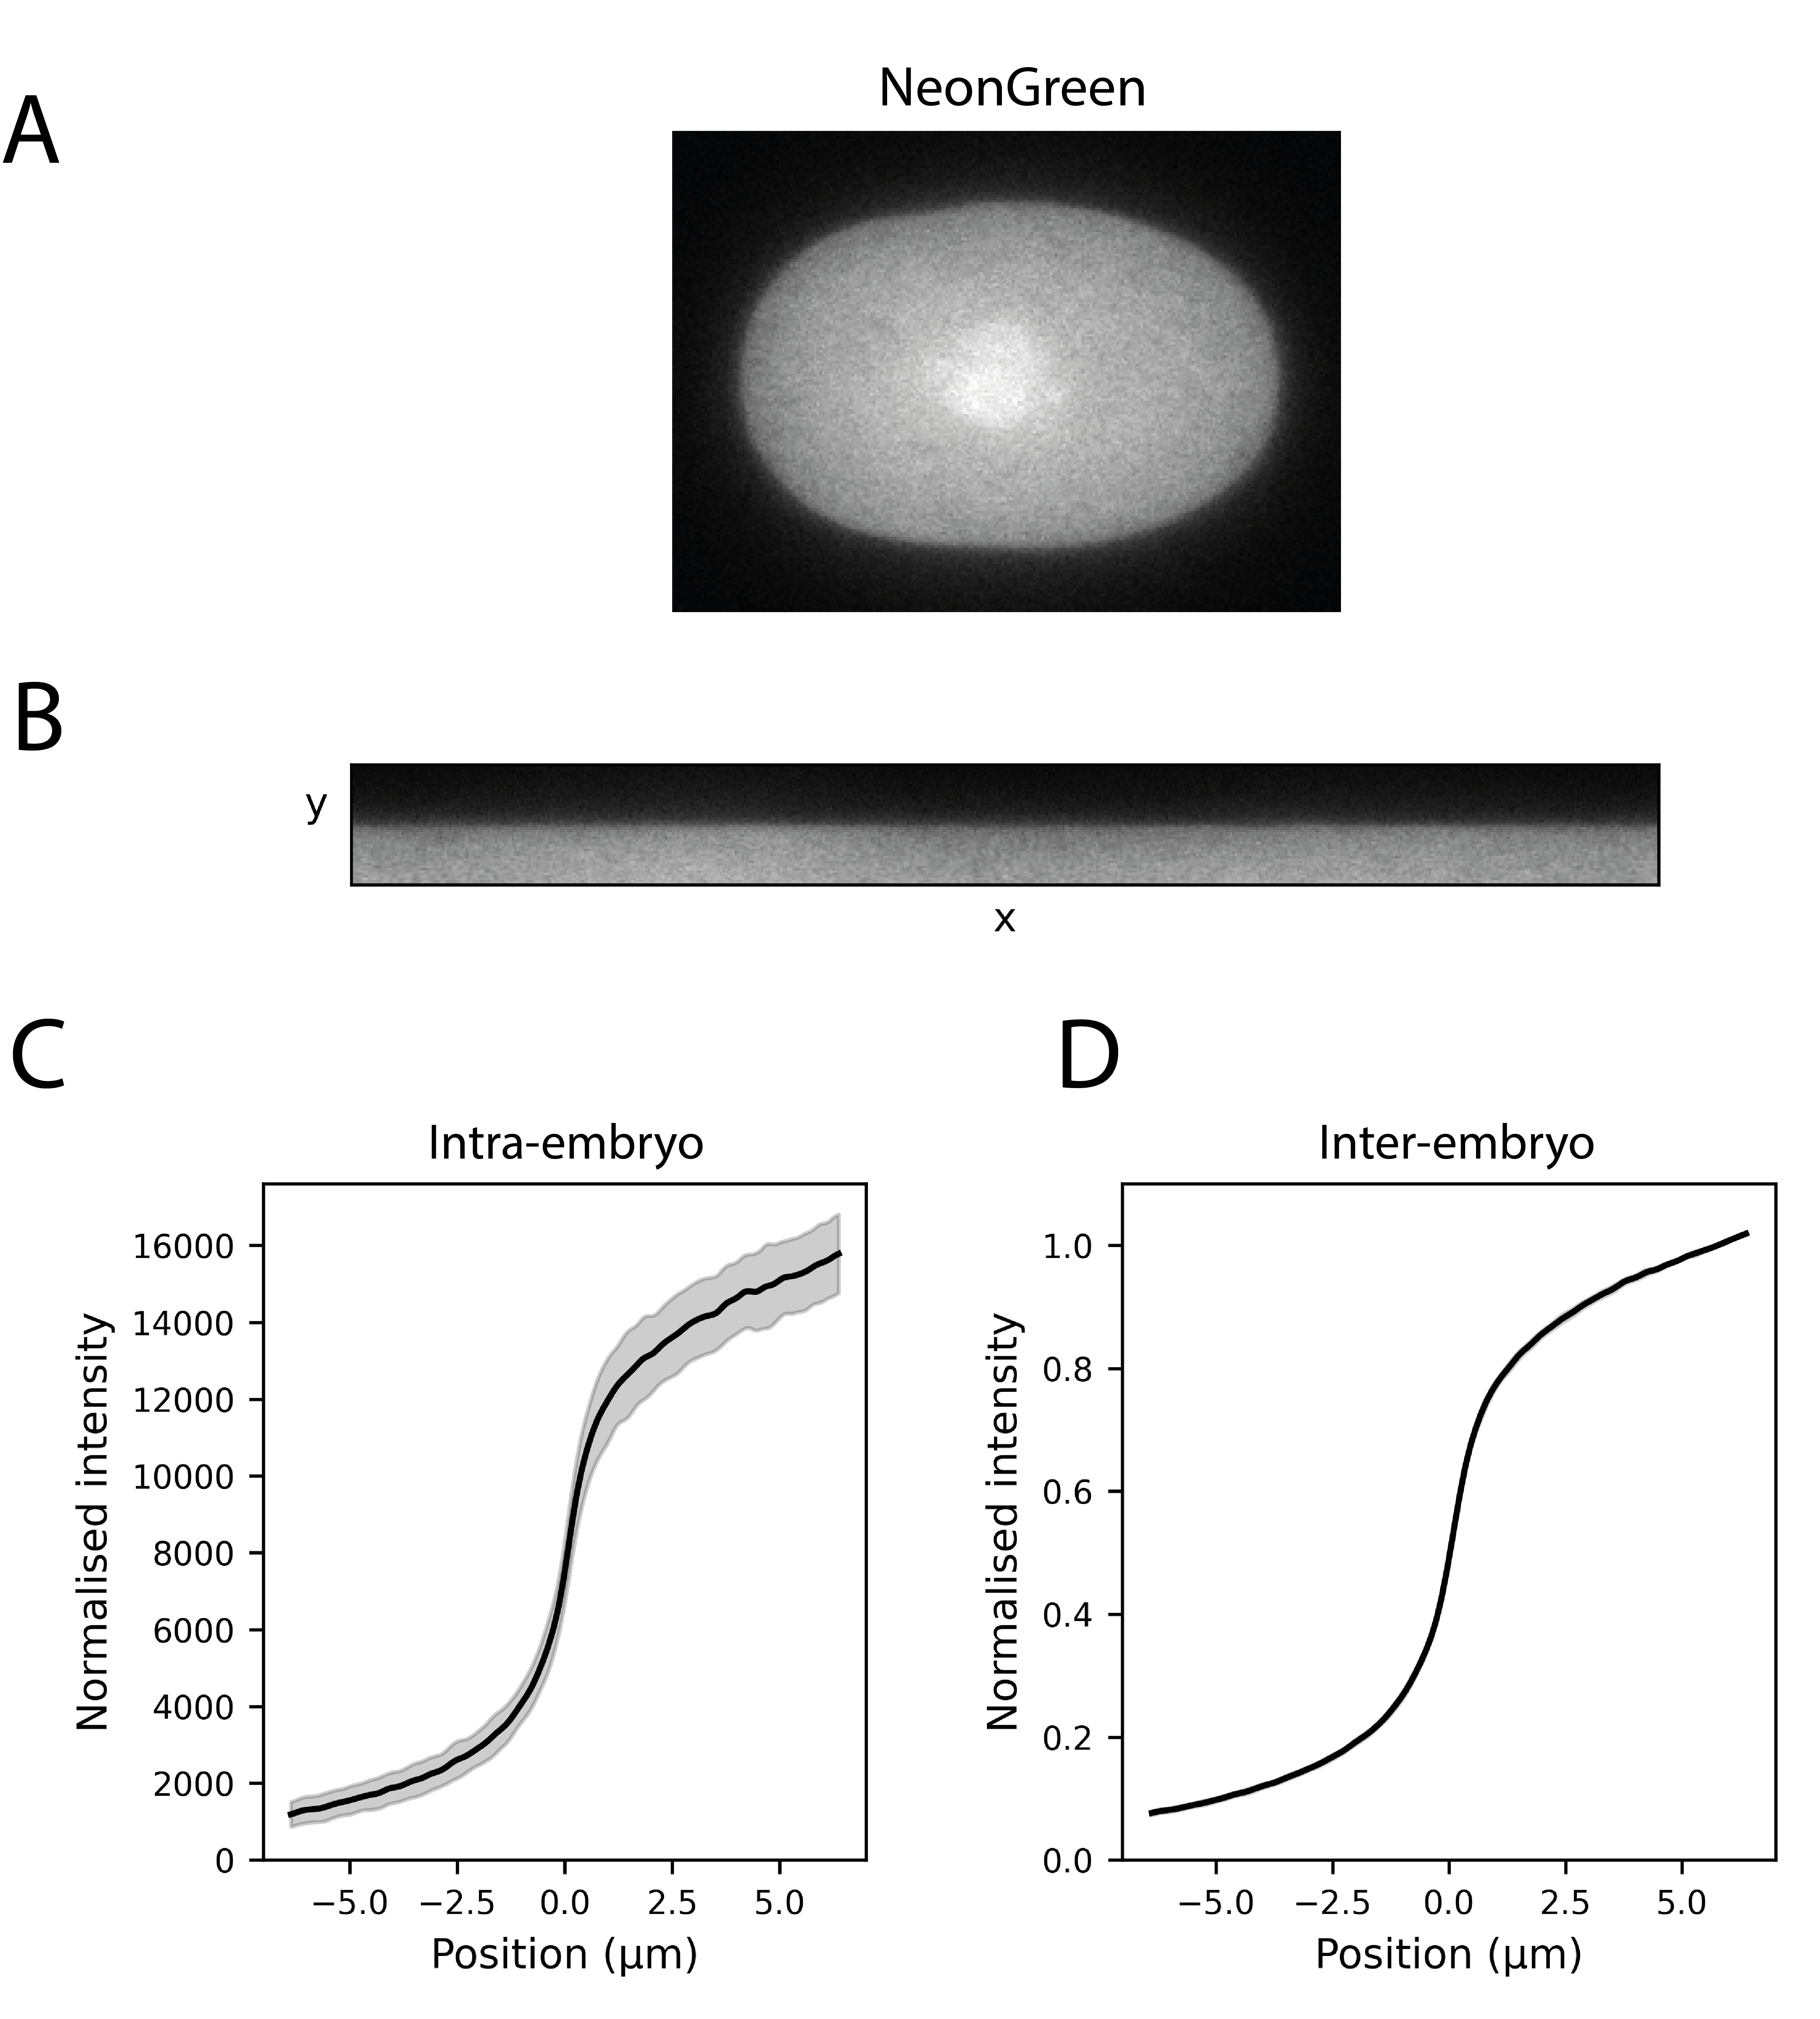
\includegraphics[scale=1]{memquant_cyt_profile}
\centering
\mycaption{Assessing the contribution of cytoplasmic protein to midplane signal}{
\textbf{(A)} Midplane image of an embryo expressing free NeonGreen.
\textbf{(B)} Straightened cortex of the image in (A).
\textbf{(C)} Straightened image in (B), averaged over the x dimension. Mean $\pm$ SD.
\textbf{(D)} Mean ($\pm$ SD) cross-cortex profile, averaged across multiple embryos.
}
\label{fig:memquant_cyt_profile}
\end{figure}

The main reason that this shape deviates so much from an error-function is likely due to scattering and diffraction of light from planes above and below the imaging plane, combined with a curved geometry in the z-dimension (\cref{fig:memquant_cyt_psf}). Scatter, which is a common issue in images of biological samples, causes a broadening of light in three dimensions as it passes through regions of heterogeneous refractive index. This occurs within the (xy) plane of an image, but is typically far more significant in the z-axis. Whilst confocal microscopes are designed to only capture light from a single plane, the whole sample is illuminated, so they will inevitably capture some emitted light from other planes that scatters into the focal plane. This means that pixel intensities within the focal plane will be affected not only by structures within that plane but also structures above and below.\\


\begin{figure}
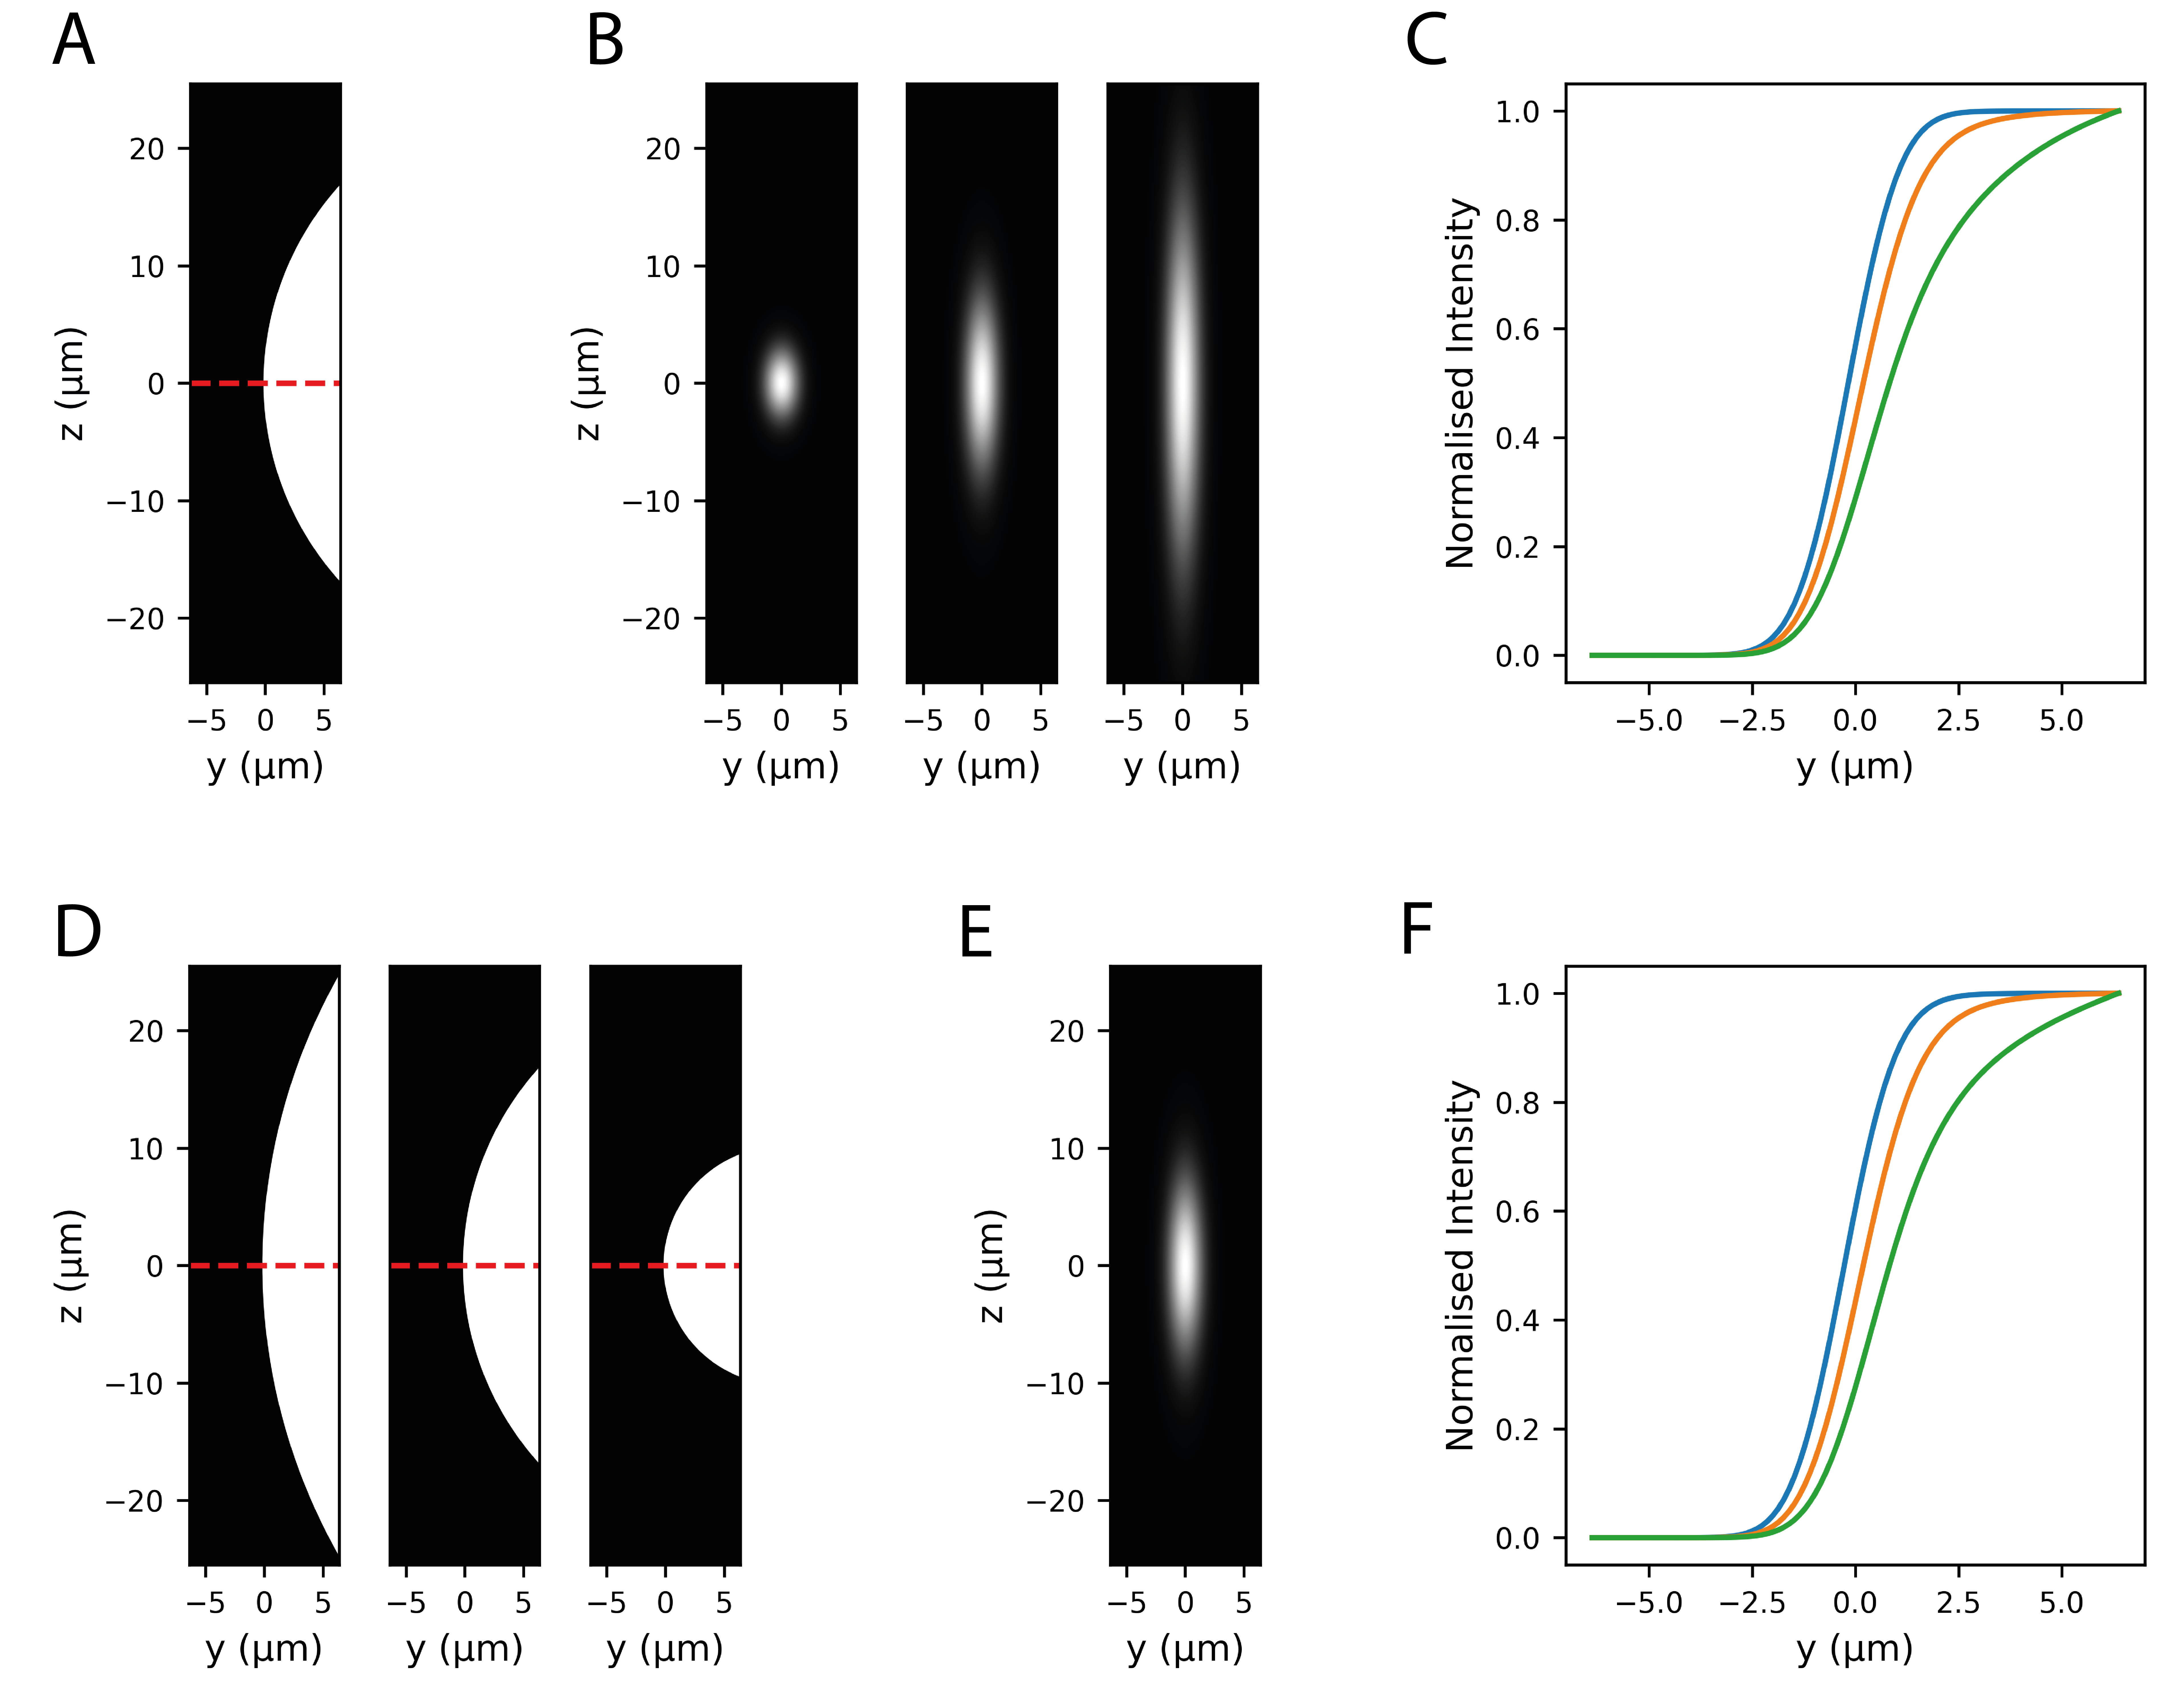
\includegraphics[scale=0.9]{memquant_cyt_psf}
\centering
\mycaption{Effects of sample geometry and the PSF on in-plane signal measurements in simulations of cytoplasm-like signal}{
\textbf{(A) - (C)} (C) shows simulated midplane signals derived from the geometry shown in (A) convolved with three different point spread functions (B).
\textbf{(D) - (F)} (F) shows simulated midplane signals derived from three geometries shown in (D) convolved with the point spread function shown in (E). Geometries are designed to resemble cytoplasmic protein at the edge of a curved cell. Red dashed lines in (A) and (D) indicate midplane. PSFs are modelled as 2D Gaussians for demonstrative purposes, and are not intended to be accurately representative of real PSFs.
}
\label{fig:memquant_cyt_psf}
\end{figure}

It is likely that a similar problem also applies in the case of membrane proteins (\cref{fig:memquant_mem_psf}). Specifically, this analysis shows that out of focus membrane signal might be expected to lead to a shape resembling an asymmetric Gaussian, with higher signal at the interior of the cell than the exterior. In fact, this phenomenon can be observed just by looking at images of polarised PAR proteins (e.g. \cref{fig:memquant_method_comparison} for PAR-2), where out-of-focus membrane signal can create the appearance of a cytoplasmic gradient. By comparison, two-photon images of PAR-2, which aim to eliminate out of focus excitation, show a completely flat cytoplasm \citep{Petrasek2008}, which is expected for most PAR proteins based on fast measured diffusion rates (although exceptions do exist, such as PAR-1, where true cytoplasmic gradients have been observed \citep{Griffin2011, Folkmann2019}). Whilst in some cases this out-of-focus bleedthrough may be of little concern, it might be particularly problematic if accurate cytoplasmic quantification is required, as this out of focus signal may be attributed to cytoplasmic protein. Without accurate measure of cytoplasmic concentrations, measures of membrane to cytoplasmic ratios, which are often used as a read-out of membrane affinity, may be wildly off. This will prove significant for much of the analysis in later chapters of this thesis.\\

\begin{figure}
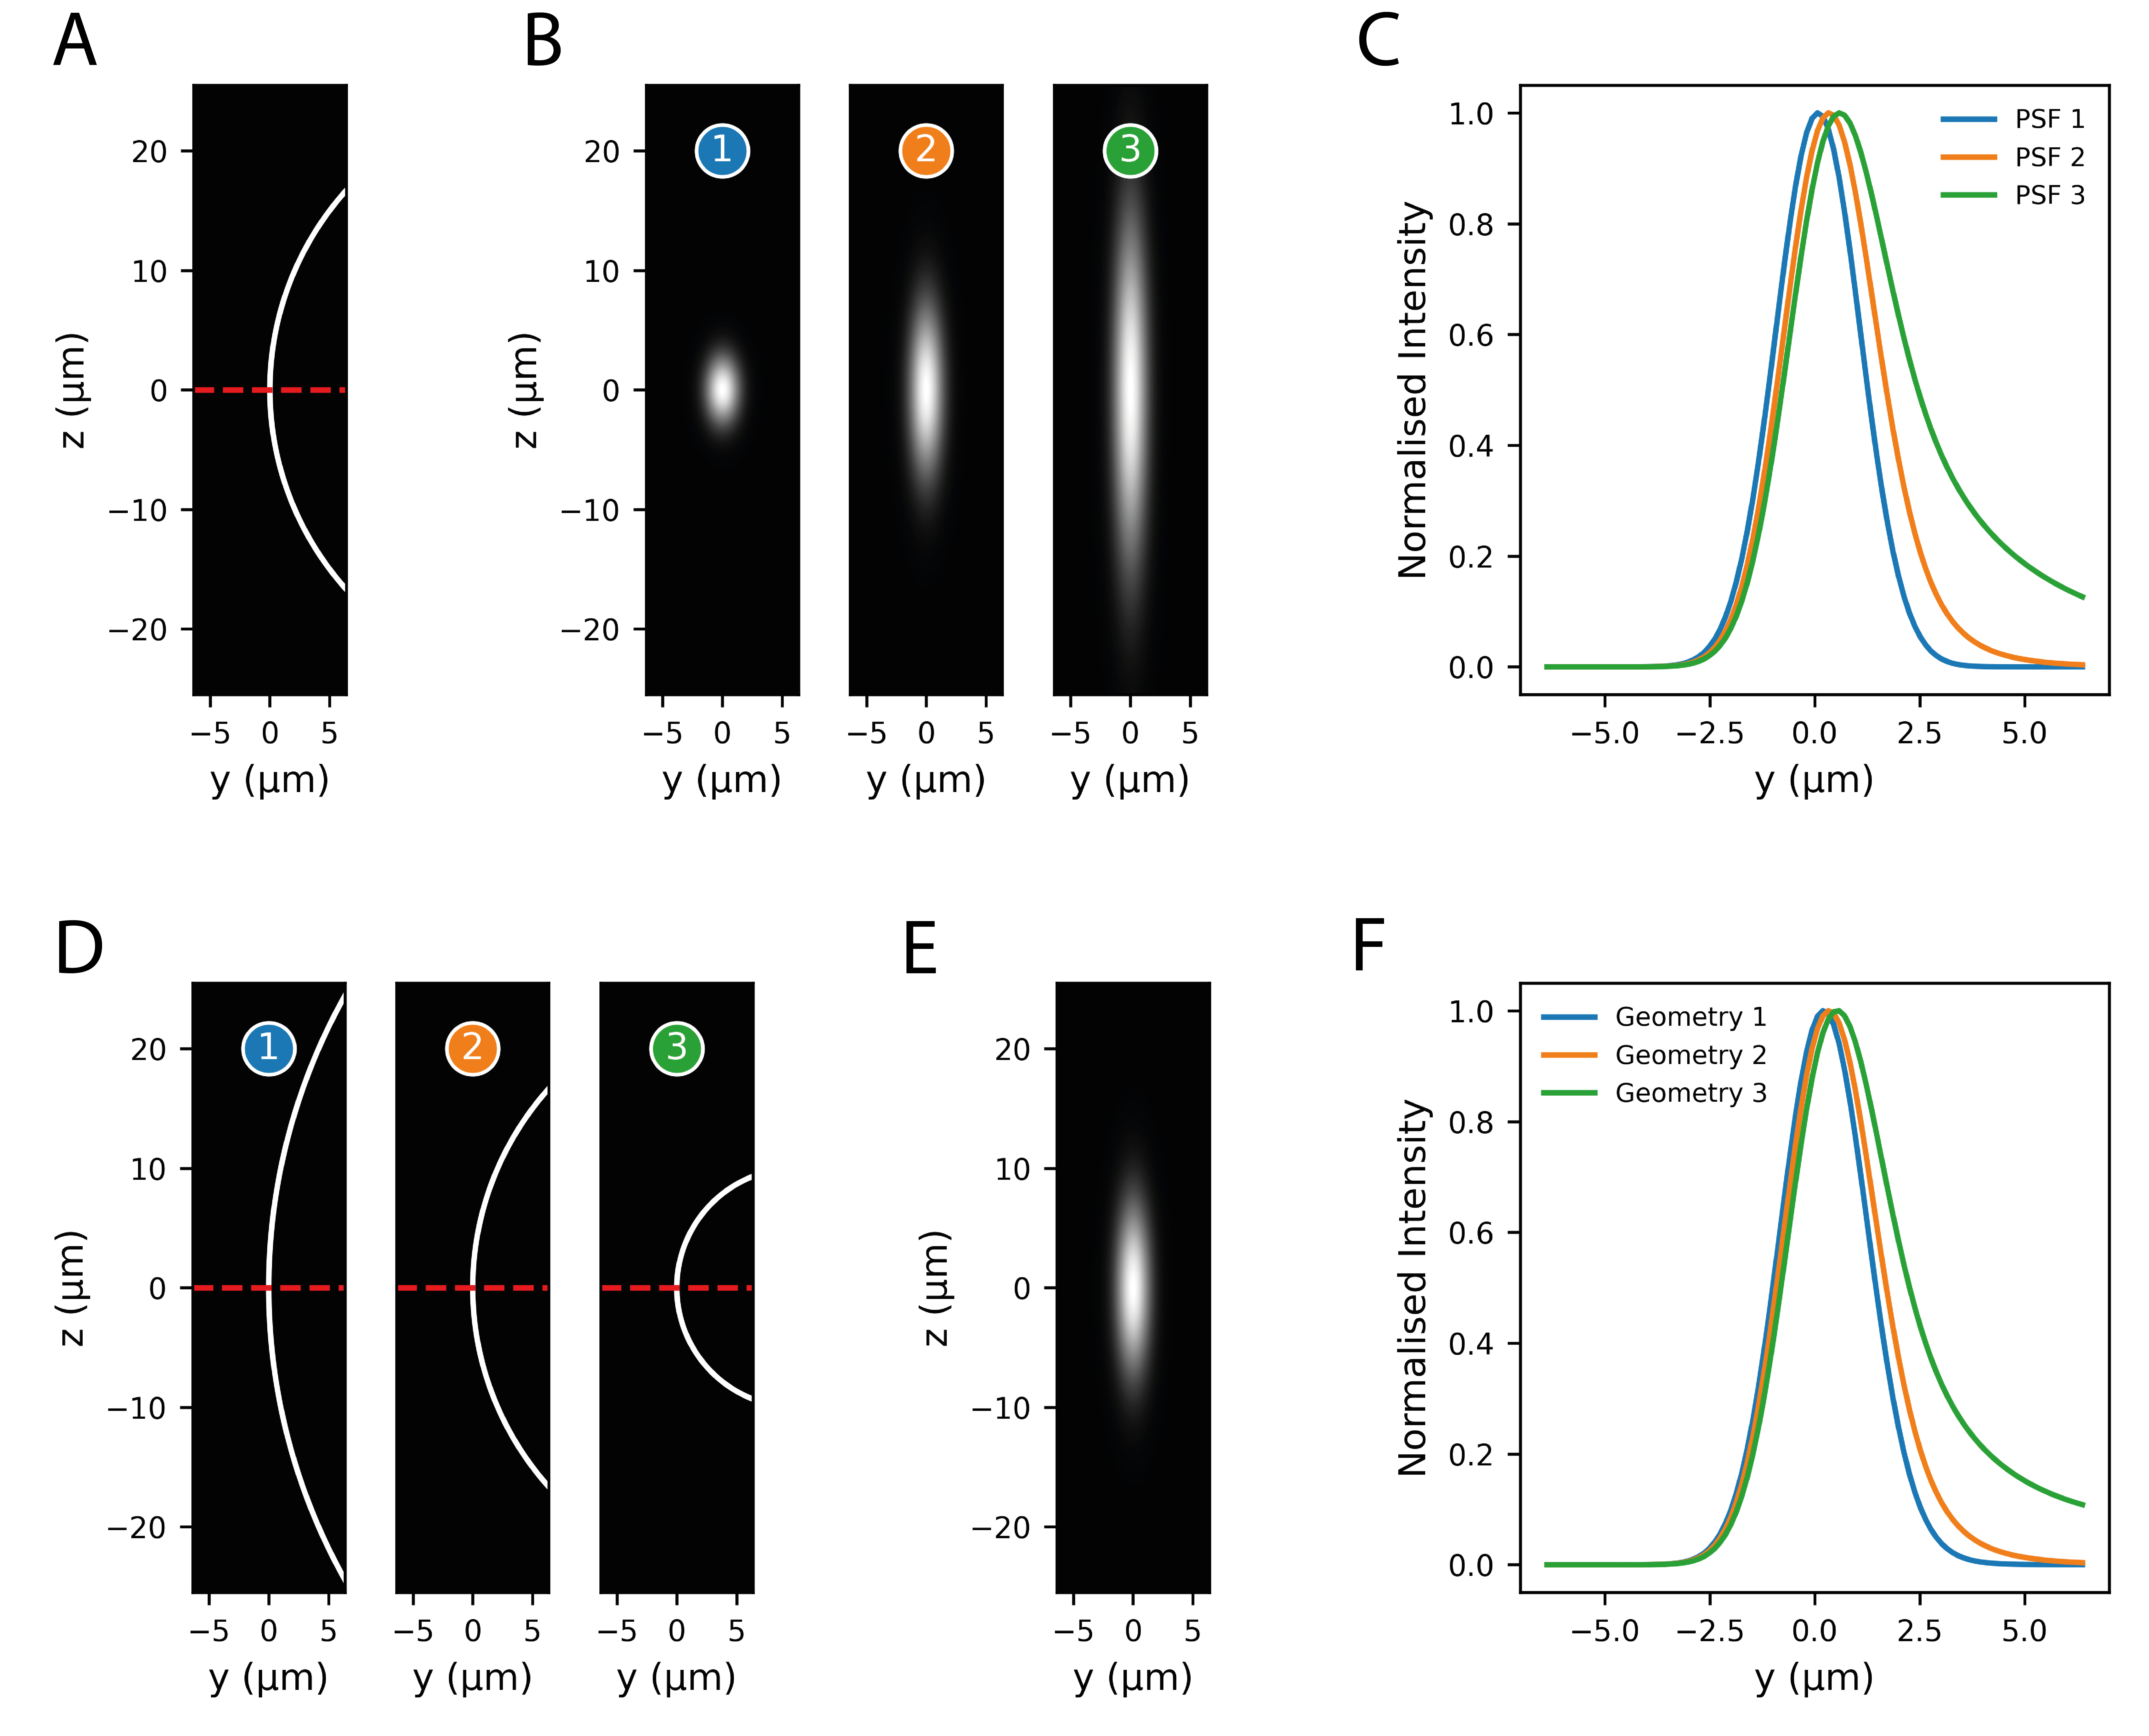
\includegraphics[scale=0.9]{memquant_mem_psf}
\centering
\mycaption{Effects of sample geometry and the PSF on in-plane signal measurements in simulations of membrane-like signal}{
\textbf{(A) - (C)} (C) shows simulated midplane signals derived from the geometry shown in (A) convolved with three different point spread functions (B).
\textbf{(D) - (F)} (F) shows simulated midplane signals derived from three geometries shown in (D) convolved with the point spread function shown in (E). Geometries are designed to resemble membrane protein at the edge of a curved cell. Red dashed lines in (A) and (D) indicate midplane. PSFs are modelled as 2D Gaussians for demonstrative purposes, and are not intended to be accurately representative of real PSFs.
}
\label{fig:memquant_mem_psf}
\end{figure}

Thus, if we want to obtain accurate measures of cytoplasmic and membrane protein concentrations, we need a method that can account for out-of-focus scatter. One common approach to account for out-of-focus scatter is to take a z-stack across the whole sample and apply a deconvolution algorithm to the 3D stack to reassign all blurred/scattered light to an in-focus location \citep{Wallace2001}. These methods rely on prior knowledge of the point spread function (PSF) that applies to the particular sample and imaging set-up, which needs to be as accurate as possible, otherwise artefacts can arise. Theoretical methods exist to estimate an appropriate PSF given parameters such as the imaging modality, numerical aperture and emitted light wavelength. However, whilst these methods are good at describing blur within the imaging apparatus, scattering within the sample and at the sample-apparatus interface is difficult to model accurately. For this reason, it can be more effective to measure an empirical PSF by imaging the 3D light distribution from a single point source (e.g. a fluorescent bead) under similar sample prep conditions to the sample of interest. However, as PSFs are influenced by scatter within the sample itself, the accuracy of this method depends on how closely the sample environment can be replicated when imaging the beads, which is not trivial. \\

Furthermore, most deconvolution methods assume that the PSF is a constant function throughout the whole image, but in many cases this will not be the case. There may, for example, be refractive index gradients within the sample, which will alter the shape of the PSF depending on location within the sample. Additionally, if there is a mismatch between the refractive index of the immersion and mounting media, as is often unavoidable when imaging live biological samples, then the PSF will usually vary with depth as spherical aberrations will be introduced deeper into the sample. A PSF from a fluorescent bead located directly below the coverslip will not capture either of these phenomena.\\

In reality, given all of these confounding factors, an accurate description of the PSF that applies to a given sample of interest is often unachievable in practice. Whilst deconvolution with a suboptimal PSF may be sufficient for many qualitative applications, accurate quantitative measurements cannot be guaranteed. For this reason, I opted against using a PSF-based deconvolution approach to account for out-of-plane scattering.\\

Fortunately, in this particular case, matters are simplified by the fact that the geometries of protein distribution are usually highly consistent. Not only is the shape of embryos highly consistent, but PAR protein distributions within the embryo also tend to display rotational symmetry (at least during normal polarity development in P0), meaning that protein distributions in planes above and below the focal plane tend to be similar/identical to those seen at the focal plane (much like the simulations in \cref{fig:memquant_cyt_psf} and \cref{fig:memquant_mem_psf}). Optical properties are also not expected to change from sample to sample, or from location to location around the circumference of an embryo.\\

Together, these features imply that, in cases where protein is either entirely cytoplasmic or entirely membrane-bound, the normalised shape of the cross-cortex profile measured at the midplane should be some constant function, that should not vary much between embryos or spatially around the circumference of an embryo. A change in local or global concentrations should amount to a rescaling of these profiles, but should not change their normalised shape. Where there is a mix of cytoplasmic and membrane protein, the total measured cross-cortex profile will then be a sum of these two contributions. Therefore, if one has prior knowledge of the expected shape of the cross-cortex profile for cytoplasmic-only and membrane-only protein, then measured profiles can be fit as the sum of these two contributions, and membrane/cytoplasmic concentrations can be extracted as the amplitudes of the two signal components.\\

Therefore, a key step in the path to accurate quantification is the ability to measure appropriate reference profiles describing the contributions of cytoplasmic and membrane protein. As mentioned previously, cytoplasmic reference profiles can easily be obtained by analysing cells in which all protein is cytoplasmic (\cref{fig:memquant_cyt_profile}). \textcite{Reich2019} (fully described in \textcite{Reich2019a}) used an approach half-way between the \textcite{Gross2018} method and the method that I am proposing, replacing the error-function description of cytoplasmic signal with a measured cytoplasmic reference profile. Thus, total signals were fit as the sum of a Gaussian profile and this reference profile, which resulted in a better ability of the model to fit the shape of measured profiles.\\

Whilst this move is a significant step in the right direction, the problem remains of how best to account for out of focus membrane light. This presents a challenge: whilst it is relatively easy to directly measure a cytoplasmic reference profile (you just need a reference image in which all signal is cytoplasmic), the same is not true for a membrane profile as it is difficult to find a reference case in which all protein is membrane bound. To extend the method to account for out-of-focus membrane protein, I attempted to find alternative methods to get an approximation of the membrane reference profile. An initial idea, which involved staining the exterior of the embryo eggshell with a fluorescent dye, proved technically challenging and not reproducible.\\

Instead, the problem becomes simplified when one considers that, even in cases where the membrane is polarised, the cytoplasmic pool of most PAR proteins should be uniform. Thus, full straightened cortices can be modelled the sum of a uniform cytoplasmic component (defined by a cytoplasmic reference profile ($R_c$) and a single, uniform, cytoplasmic concentration ($C$)) and a polarised membrane component (defined by a membrane reference profile ($R_m$) and a nonuniform membrane concentration profile ($M$)), as shown in \cref{fig:memquant_model_schematic}. This is essentially a generalisation of the \textit{Fitting based quantification} method presented in \cref{fig:memquant_method_comparison}, but proposes the use of arbitrary membrane and cytoplasmic reference profiles rather than mathematical functions (e.g. Gaussian, error function), and has the restriction of a uniform cytoplasm across the embryo.\\

\begin{figure}
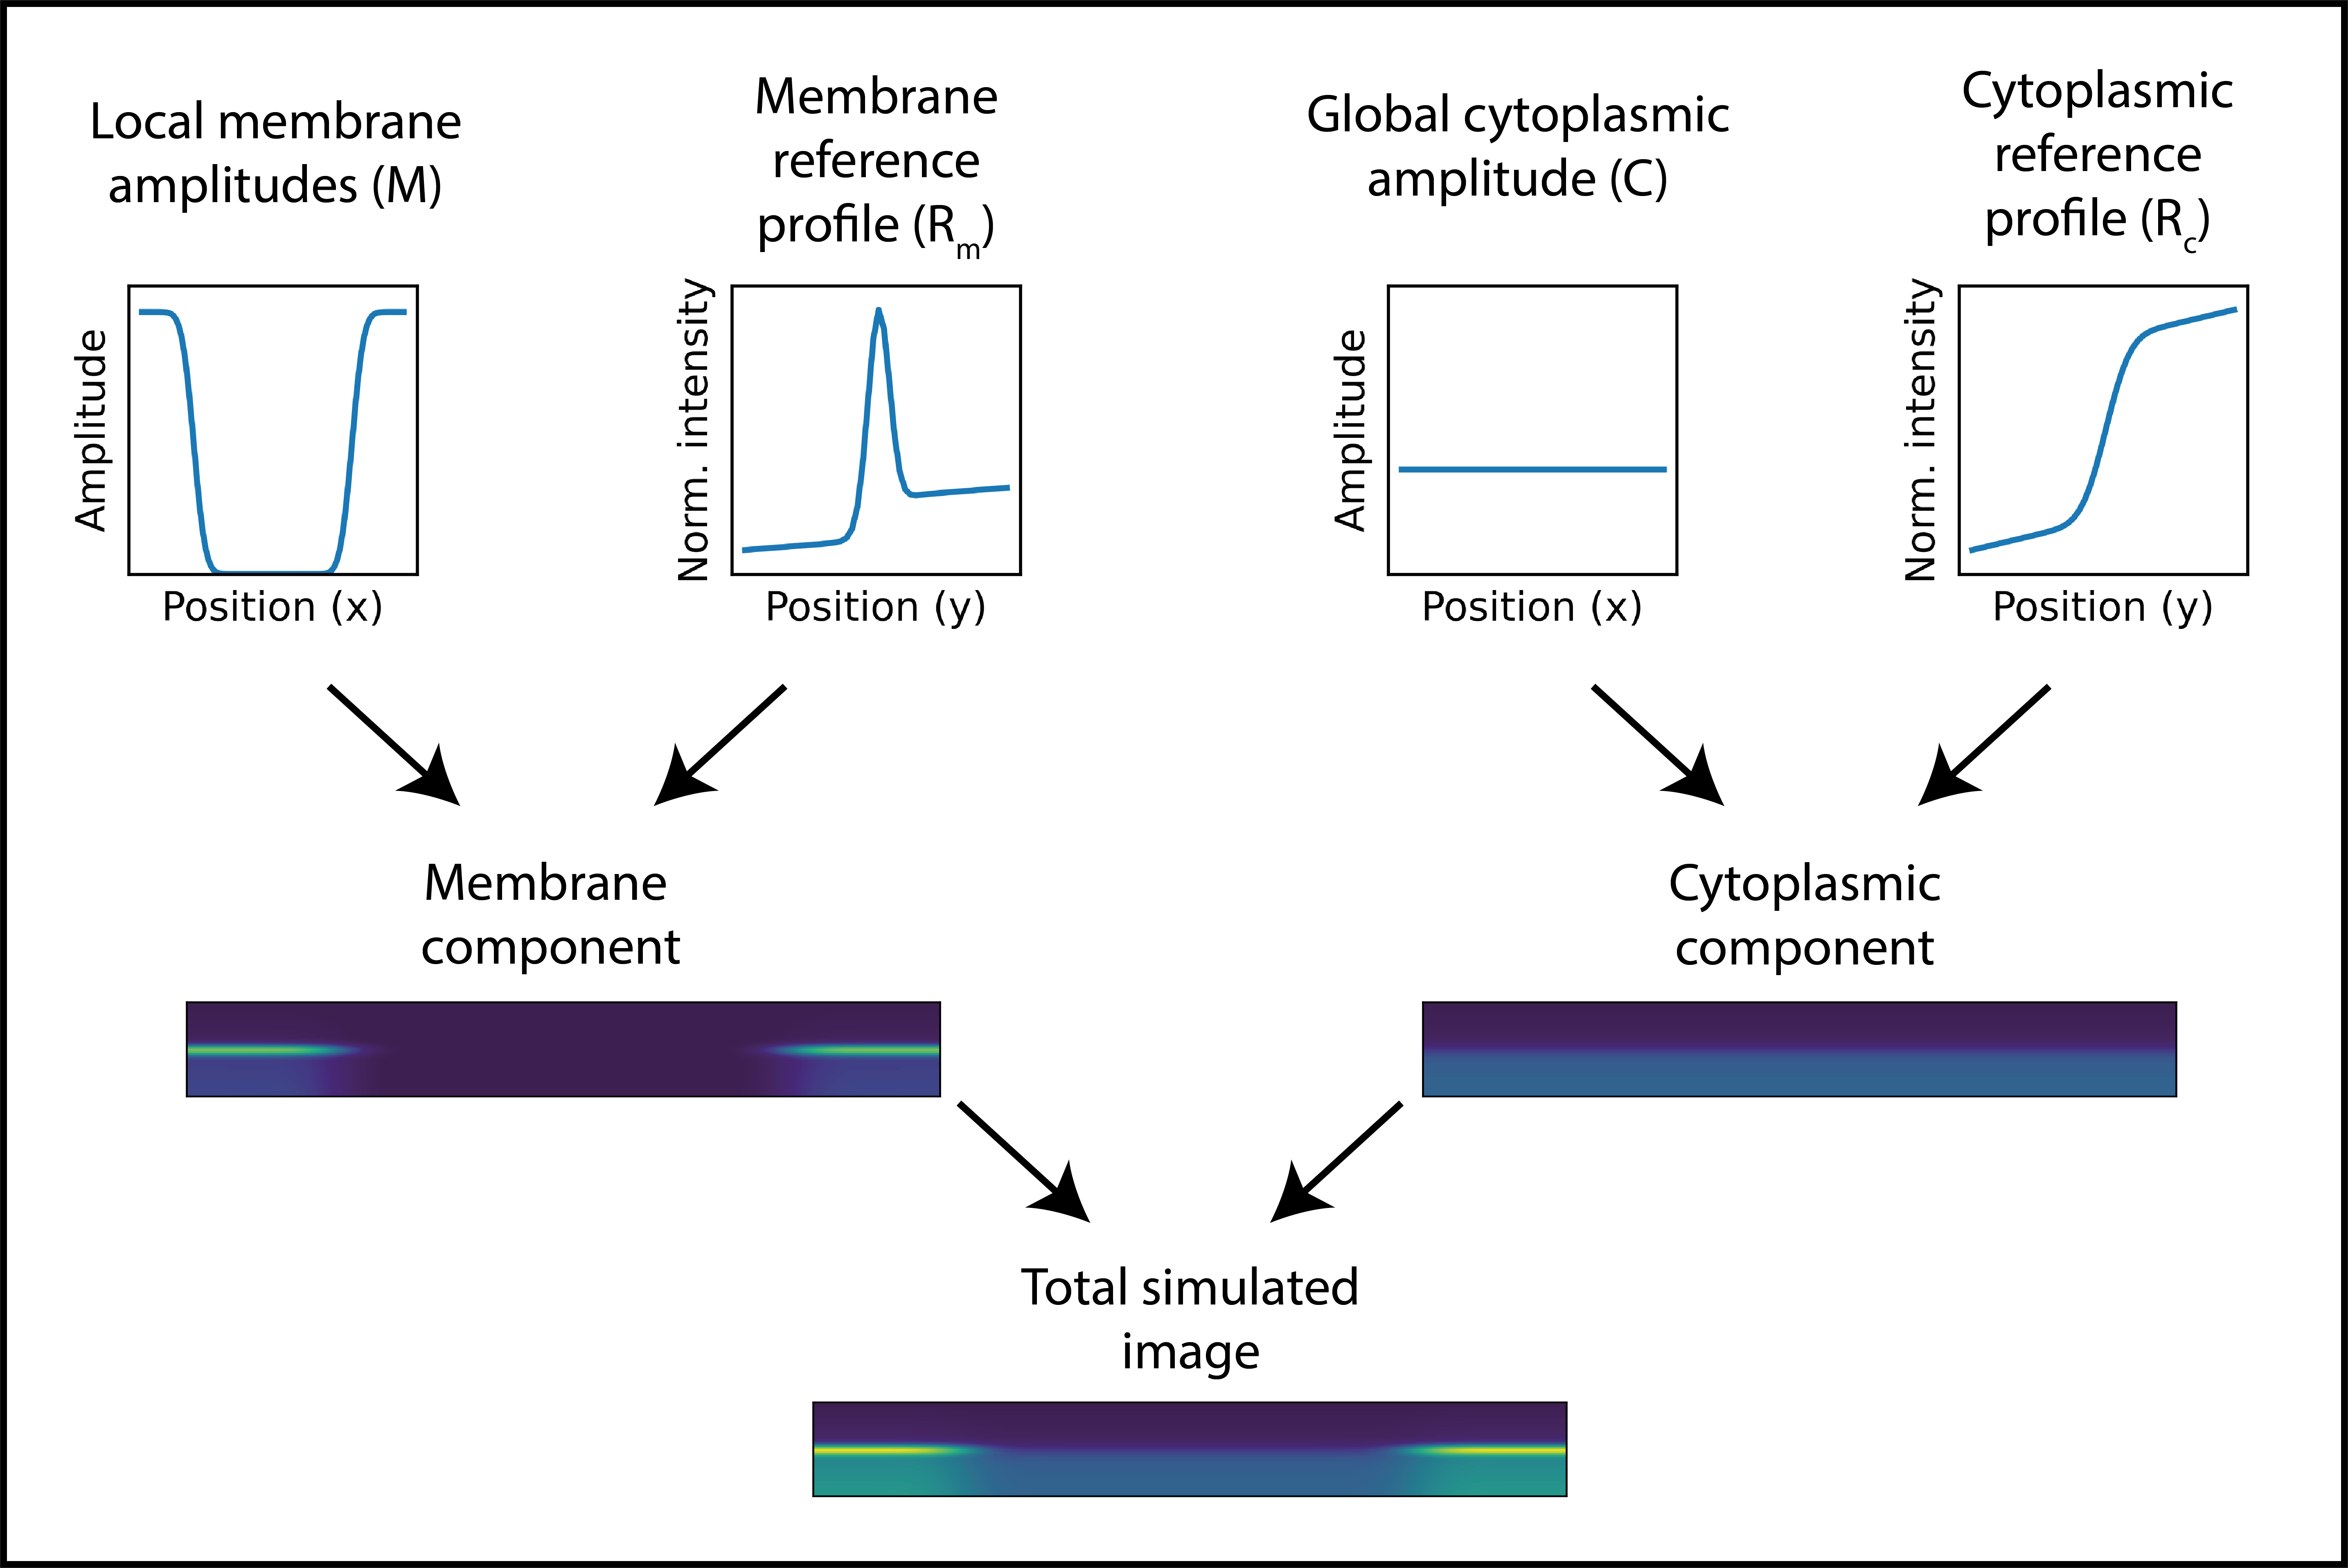
\includegraphics[scale=1.15]{memquant_model_schematic}
\centering
\mycaption{A model for simulating membrane and cytoplasmic fluorescence signal at the cortex}{
Simulated images of straightened cortices are described as the sum of membrane and cytoplasmic signal components. The membrane component is described as a 1D array of amplitudes ($M$), representing concentrations around the circumference of the embryo, convolved with a membrane reference profile ($R_m$). The cytoplasmic component is described as a single uniform amplitude ($C$) convolved with a cytoplasmic reference profile ($R_c$). Blur/scatter in the x dimension is ignored as adjacent positions are assumed to be similar.
}
\label{fig:memquant_model_schematic}
\end{figure}

$R_c$ can easily be predefined by imaging embryos in which all protein is cytoplasmic (\cref{fig:memquant_cyt_profile}). If we assume for now that $R_m$ is also predefined, then $M$ and $C$ for a given embryo can be determined by fitting a straightened image to the model presented in \cref{fig:memquant_model_schematic}. (At this point concentrations will be in arbitrary units, but I will return to this point later). Whilst $R_m$ is in fact not predefined, given the constraints imposed by cytoplasmic uniformity, only a model with an appropriate $R_m$ will be able to create simulated images that closely match experimental images. (Imagine, for example a model with a Gaussian membrane reference profile, which would clearly fail to capture graded interior signal). Therefore, under conditions such as these, in which we have a uniform cytoplasmic component and a graded membrane component, $R_m$ need not be predefined, and can simply be fit to the data along with the concentration parameters. To perform this kind of optimisation, I developed a gradient descent approach based on differentiable programming, which I describe below.\\


\subsection{A gradient descent protocol for image quantification}

Gradient descent is a popular optimisation strategy used for a number of machine learning applications. When optimising a model described by a series of parameters, the idea of gradient descent is to calculate the partial derivative of each parameter with respect to a loss term such as mean squared error (MSE). A negative gradient for a certain parameter would imply that an increase in that parameter would decrease the loss term, whereas a positive gradient would imply the opposite. Therefore, to reduce loss, each input parameter can be adjusted in proportion to the negative of its partial derivative. Starting with a set of initial conditions, this procedure is iteratively repeated, adjusting parameters and calculating new gradients at each step, until the loss term reaches a minimum. \\

The utility of these methods has been greatly advanced in recent years by the development of differentiable programming tools \citep{Abadi2016, Bradbury2018,  Paszke2019}. Commonly used for deep learning, although generalisable to other problems, these tools greatly speed up computation for complex optimisation procedures by automatically calculating gradients, rather than relying on numerical methods, using a process known as backpropagation. In addition, extensions to the basic gradient descent algorithm have proven effective at speeding up convergence and preventing entrapment in local minima \citep{Sun2019}. \\

In the case of this particular problem, the procedure is described in \cref{fig:memquant_forward_and_back_propagation}. Given a set of parameters ($M$, $C$, $R_m$, $R_c$), a forward propagation step simulates an image, and this is compared to the ground truth image to calculate a loss term. Backpropagation then calculates the gradient of each of the input parameters with respect to this loss term. At this point, we can adjust some or all of the input parameters according to these gradients. Repeating this cycle of forward and back propagation will then lead to a gradual optimisation of these parameters, until the loss function reaches a minimum. \\

\begin{figure}
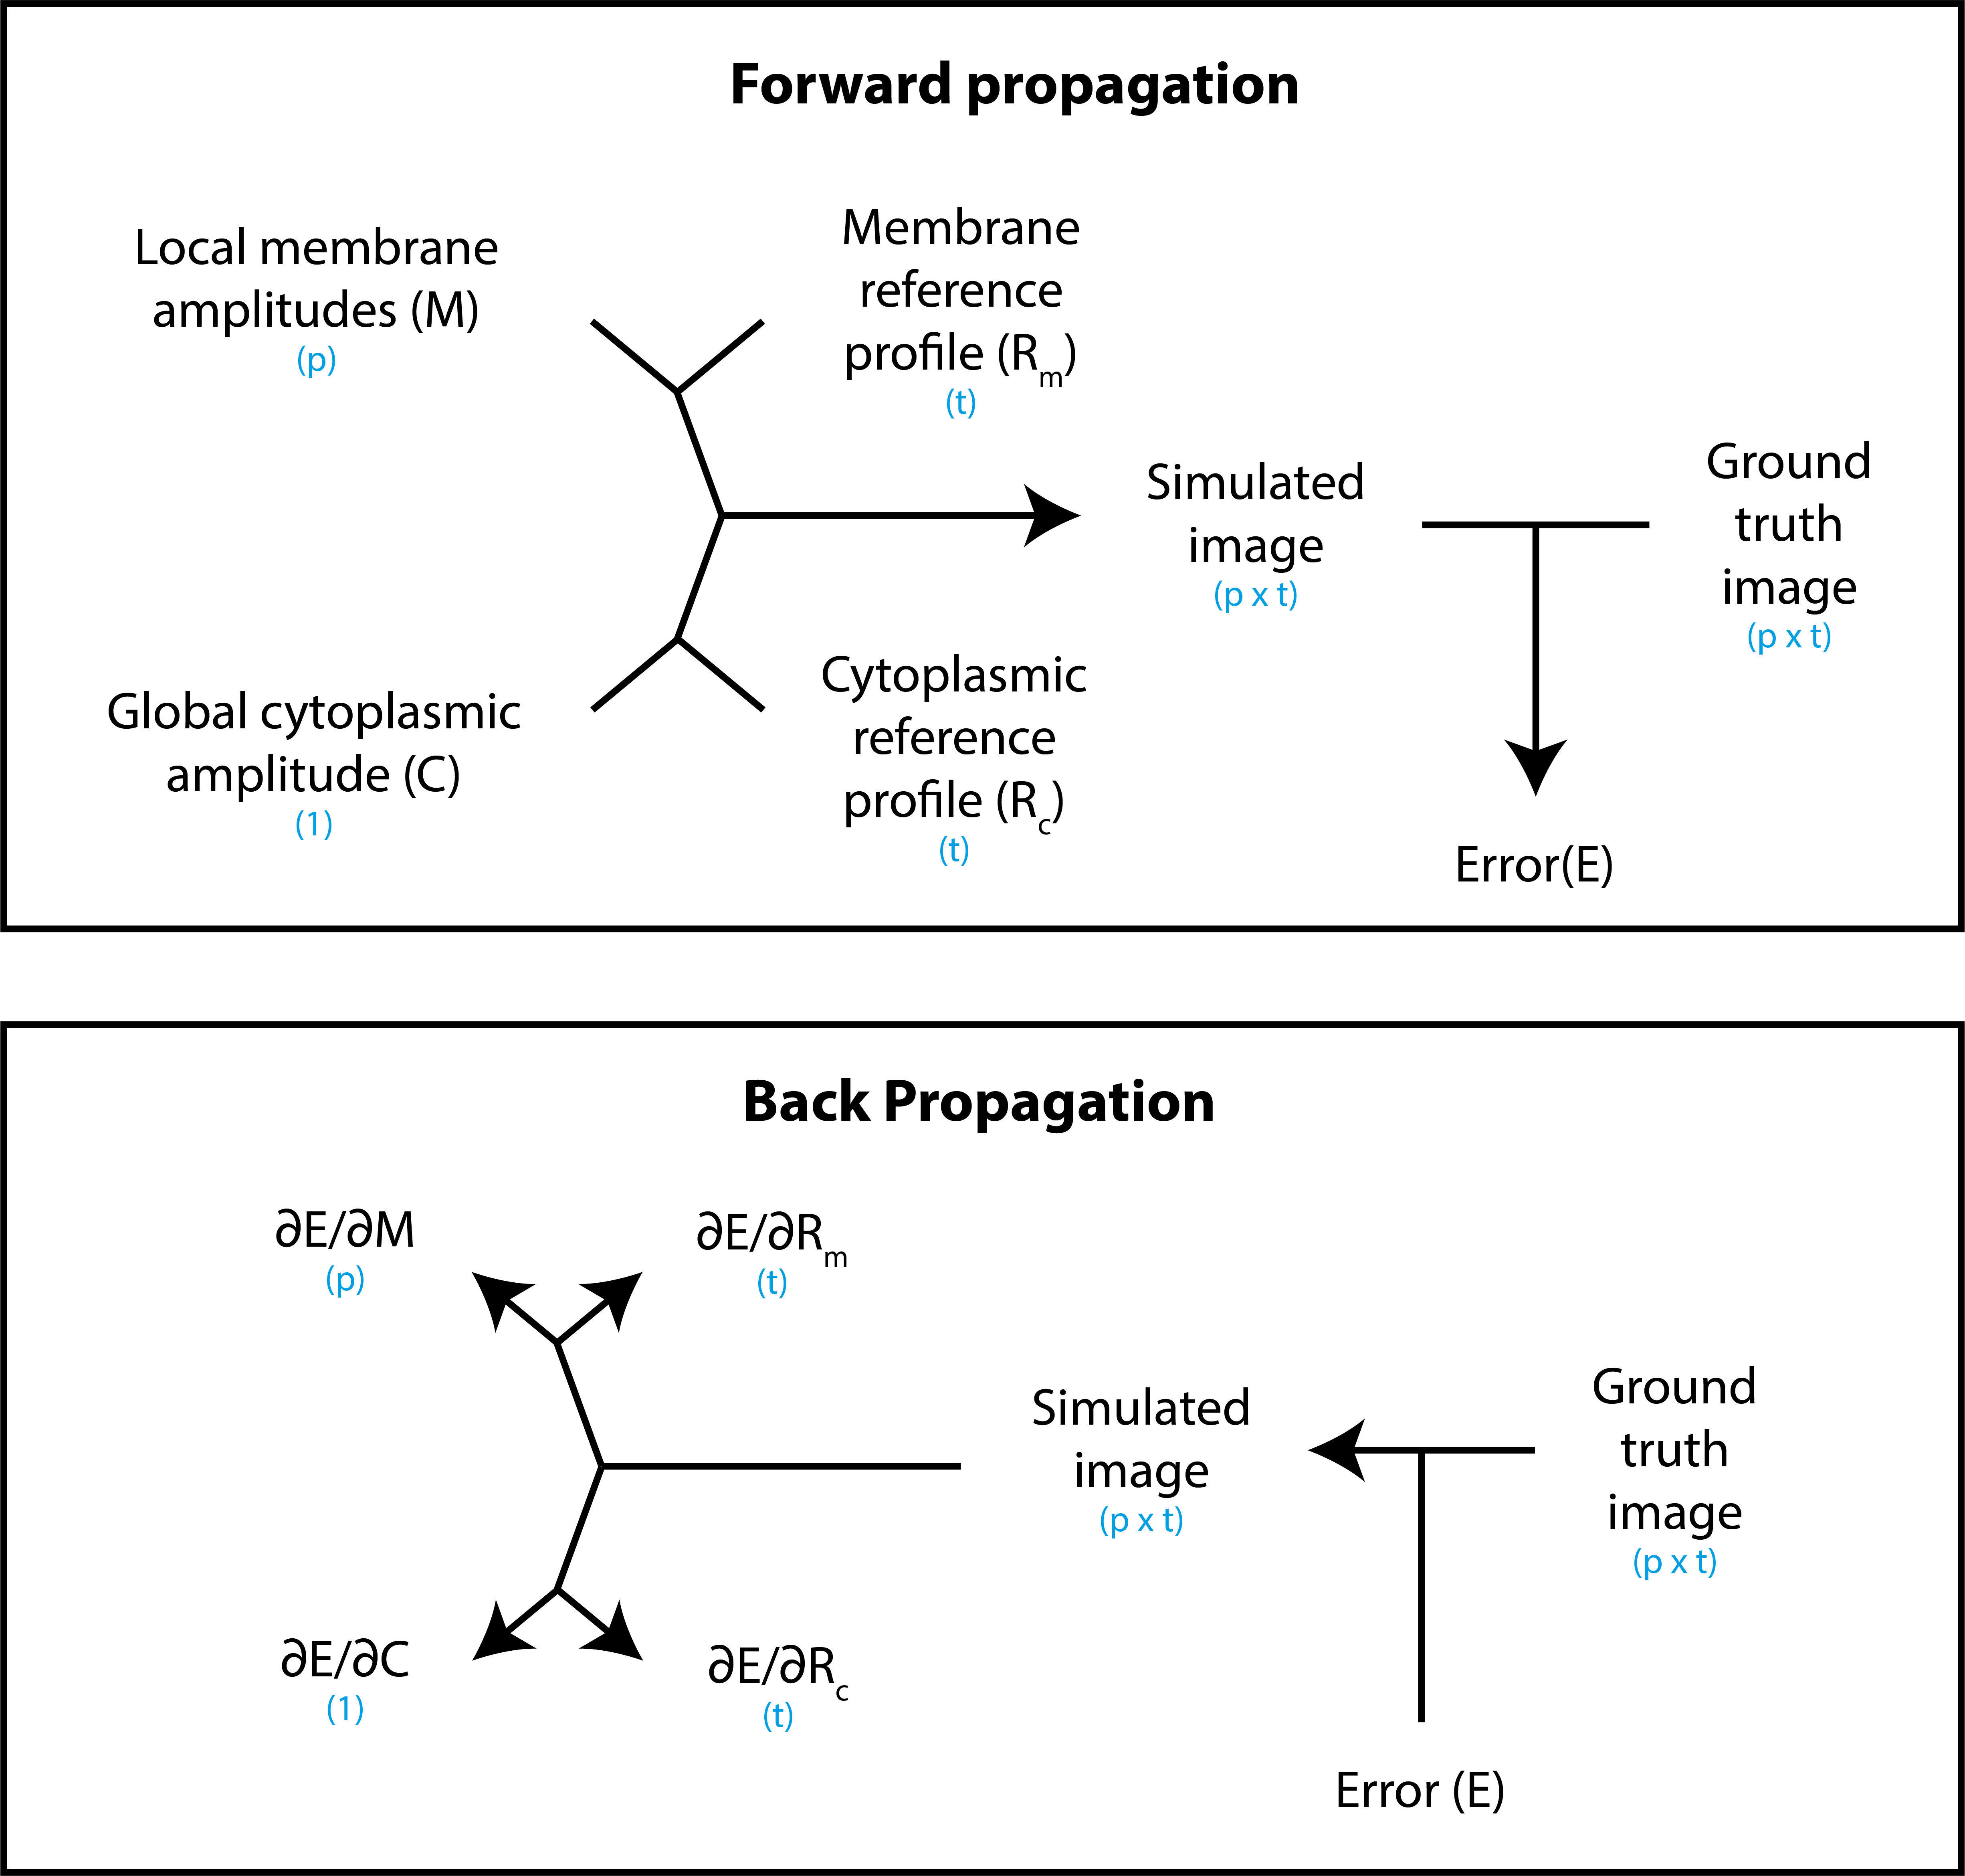
\includegraphics[scale=1.1]{memquant_forward_and_back_propagation}
\centering
\mycaption{Backpropagation gradient descent protocol for parameter optimisation}{Parameters are optimised by an iterative cycle of forward and back propagation. In the forward propagation step (top), an image is simulated given input parameters $M$, $C$, $R_m$, $R_c$, and compared to the ground truth image to calculate a loss term. In the back propagation step (bottom) gradients of the loss term with respect to each of the input parameters are calculated using the chain rule method. A subset of the input parameters can then be changed according to these gradients, which will depend on the procedure (e.g. \cref{fig:memquant_membg_training} vs \cref{fig:memquant_benchmarking_ph_rundown}). This process is repeated many times until optimisation reaches a plateau. Dimensions of the variables are shown in blue, where p represents the number of positions to fit around the cortex, and t represents the thickness of the straightened image (in pixels).}
\label{fig:memquant_forward_and_back_propagation}
\end{figure}

To test this approach, I built a model using the differentiable programming package Tensorflow \citep{Abadi2016}, and first applied it to images of polarised PAR-2. The model was initiated with all concentrations ($M$ and $C$) equal to zero, and $R_m$ initiated as a Gaussian. For $R_c$ I used a measured profile (\cref{fig:memquant_cyt_profile}), and this was not adjusted during training (\cref{fig:memquant_membg_training}A). Using an Adam optimiser \citep{Kingma2015} with a learning rate of 0.01, all other parameters ($M$, $C$ and $R_m$) were then adjusted iteratively until a plateau was reached (250 steps), as shown in \cref{fig:memquant_membg_training}B. The final simulated image, composed of a uniform cytoplasmic component and a nonuniform membrane component, closely matches the ground truth image (\cref{fig:memquant_membg_training}C).\\


\begin{figure}
\includegraphics[scale=1]{memquant_membg_training}
\centering
\mycaption{Separation of membrane and cytoplasmic signal in an image of mNG::PAR-2}{
\textbf{(A)} Schematic demonstrating the optimisation procedure, highlighting the input parameters to be optimised in red.
\textbf{(B)} $R_m$, $M$ and $C$ throughout the training procedure for an mNG::PAR-2 expressing polarised embryo. $R_m$ was initiated as a Gaussian (radius = 0.5 $\mu$m) centred at zero, $M$ and $C$ initiated as zero.
\textbf{(C)} Final simulated image compared to the ground truth image. Right panel shows profiles at specified positions (solid = ground truth, dashed = simulated). Uniform cytoplasmic component shared between profiles indicated in gray.
}
\label{fig:memquant_membg_training}
\end{figure}

% more here on reproducibility.

\subsection{Segmentation}

In addition to the parameters already mentioned, the full model also includes a series of alignment parameters, which can also be trained by gradient descent, allowing the model to freely align to the ground truth straightened image in the y direction. As a result, ground truth images do not need to be accurately segmented prior to optimisation, and rough manual ROIs are fine to use. This is particularly useful for timelapse movies, where, even if the embryo undergoes shape changes, only a single manual ROI needs to be provided. An additional outcome of alignment is that the offset parameters can be used to refine the original ROI, meaning that the method can serve as a tool for computational segmentation. Refined ROIs can then be used to re-straighten the cortex, and optimisation repeated (\cref{fig:memquant_segmentation}). Overall, this allows cortices to be segmented with subpixel accuracy with minimal manual input. In theory, the initial manual step could also be automated using deep learning methods to create a fully automated pipeline \citep{Minaee2021}.\\

\begin{figure}
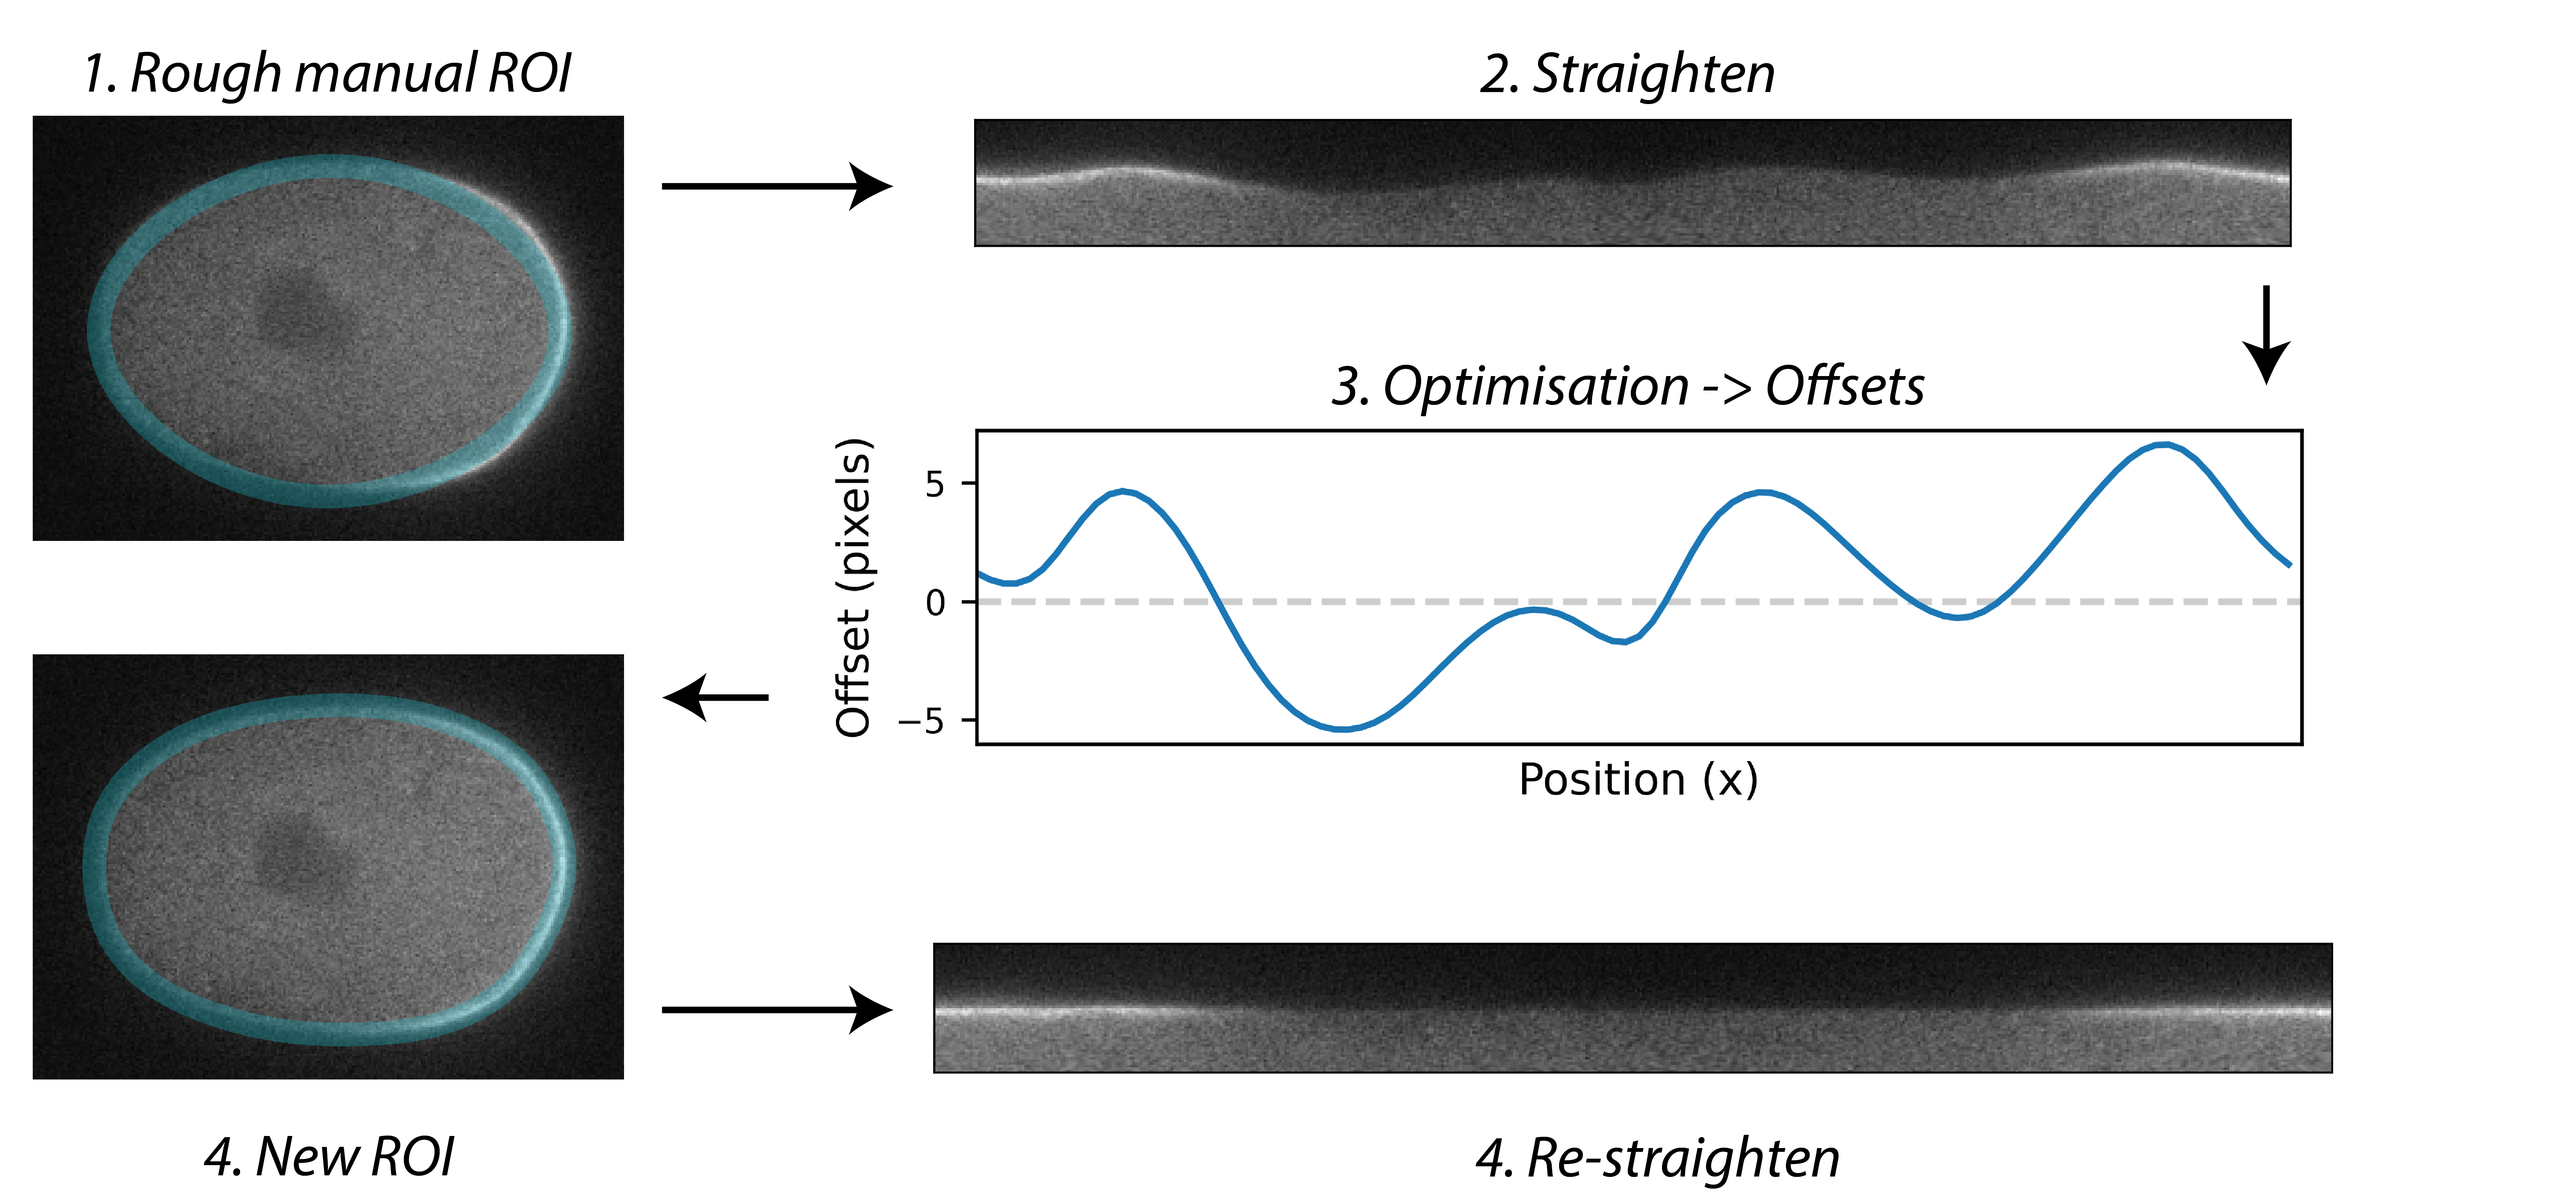
\includegraphics[scale=1]{memquant_segmentation_v2}
\centering
\mycaption{Semi-automated segmentation algorithm}{
Segmentation is initiated with a rough manual ROI. The cortex is then straightened and fit to the model yielding, among other parameters, parameters describing offset at each position along the x dimension. These offsets can then be used to adjust the initial ROI, and re-straighten the cortex. The re-straightened cortex can then be refit to the model to give concentration parameters. Shown here for an embryo expressing mNG::PAR-2(L109R).
}
\label{fig:memquant_segmentation}
\end{figure}


\subsection{Benchmarking the method}

The method described so far is limited to cases of images with polarised membranes. However, as discussed previously, $R_m$, which is a function of local geometry and optical properties, should be a constant function applicable to all embryos. Therefore, much like I used a predefined $R_c$ when fitting images of polarised PAR-2, images of proteins without a polarised membrane can be quantified by using an $R_m$ derived from a calibration procedure on polarised images. \\

To test this method, I performed quantification on images of embryos expressing the uniform plasma membrane probe GFP::PH (pleckstrin homology domain) with variable expression levels (\cref{fig:memquant_benchmarking_ph_rundown}B), obtained by performing an RNA interference (RNAi) rundown using XFP RNAi feeding bacteria (see Methods). In this case, I used a predefined $R_m$ and $R_c$, and only optimised $M$ and $C$ (as well as the alignment parameters described in the previous section) (\cref{fig:memquant_benchmarking_ph_rundown}A). Images were initiated with a rough manual ROI and segmented using the method described in \cref{fig:memquant_segmentation} prior to final quantification. Compatible with expected linear membrane binding kinetics, we can see that the method gives a tight linear relationship between cytoplasmic and membrane concentrations (\cref{fig:memquant_benchmarking_ph_rundown}C). N2s are also accurately described as having cytoplasmic and membrane concentrations close to zero.\\

\begin{figure}
\includegraphics[scale=1]{memquant_benchmarking_ph_rundown}
\centering
\mycaption{Quantification of GFP::PH expressing embryos reveals a linear relationship between membrane and cytoplasmic concentrations}{
\textbf{(A)} Schematic demonstrating the optimisation procedure, highlighting the input parameters to be optimised in red.
\textbf{(B)} Images of GFP::PH expressing embryos with varying dosages of GFP::PH, obtained by RNAi rundown.
\textbf{(C)} Membrane vs. cytoplasmic concentrations for the full dataset of embryos. Empty circles represent untagged N2 embryos. Embryos in (B) represented by blue, orange and green circles.
\textbf{(D)} Cross-cortex profiles averaged over the entire circumference of the embryo vs. GFP::PH dosage. Colour coding as in (C).
}
\label{fig:memquant_benchmarking_ph_rundown}
\end{figure}

I next investigated how robust the pipeline is to changing signal-to-noise ratios, using images of three GFP::PH embryos with varying expression levels and adding varying levels of Gaussian pixel noise (\cref{fig:memquant_benchmarking_noise}A). As seen in \cref{fig:memquant_benchmarking_noise}B and C, pixel noise adds noise to the resulting quantifications, but does not bias the data in any direction. Quantification of untagged N2s is also not biased by noise (\cref{fig:memquant_benchmarking_noise}B/C grey points).\\

\begin{figure}
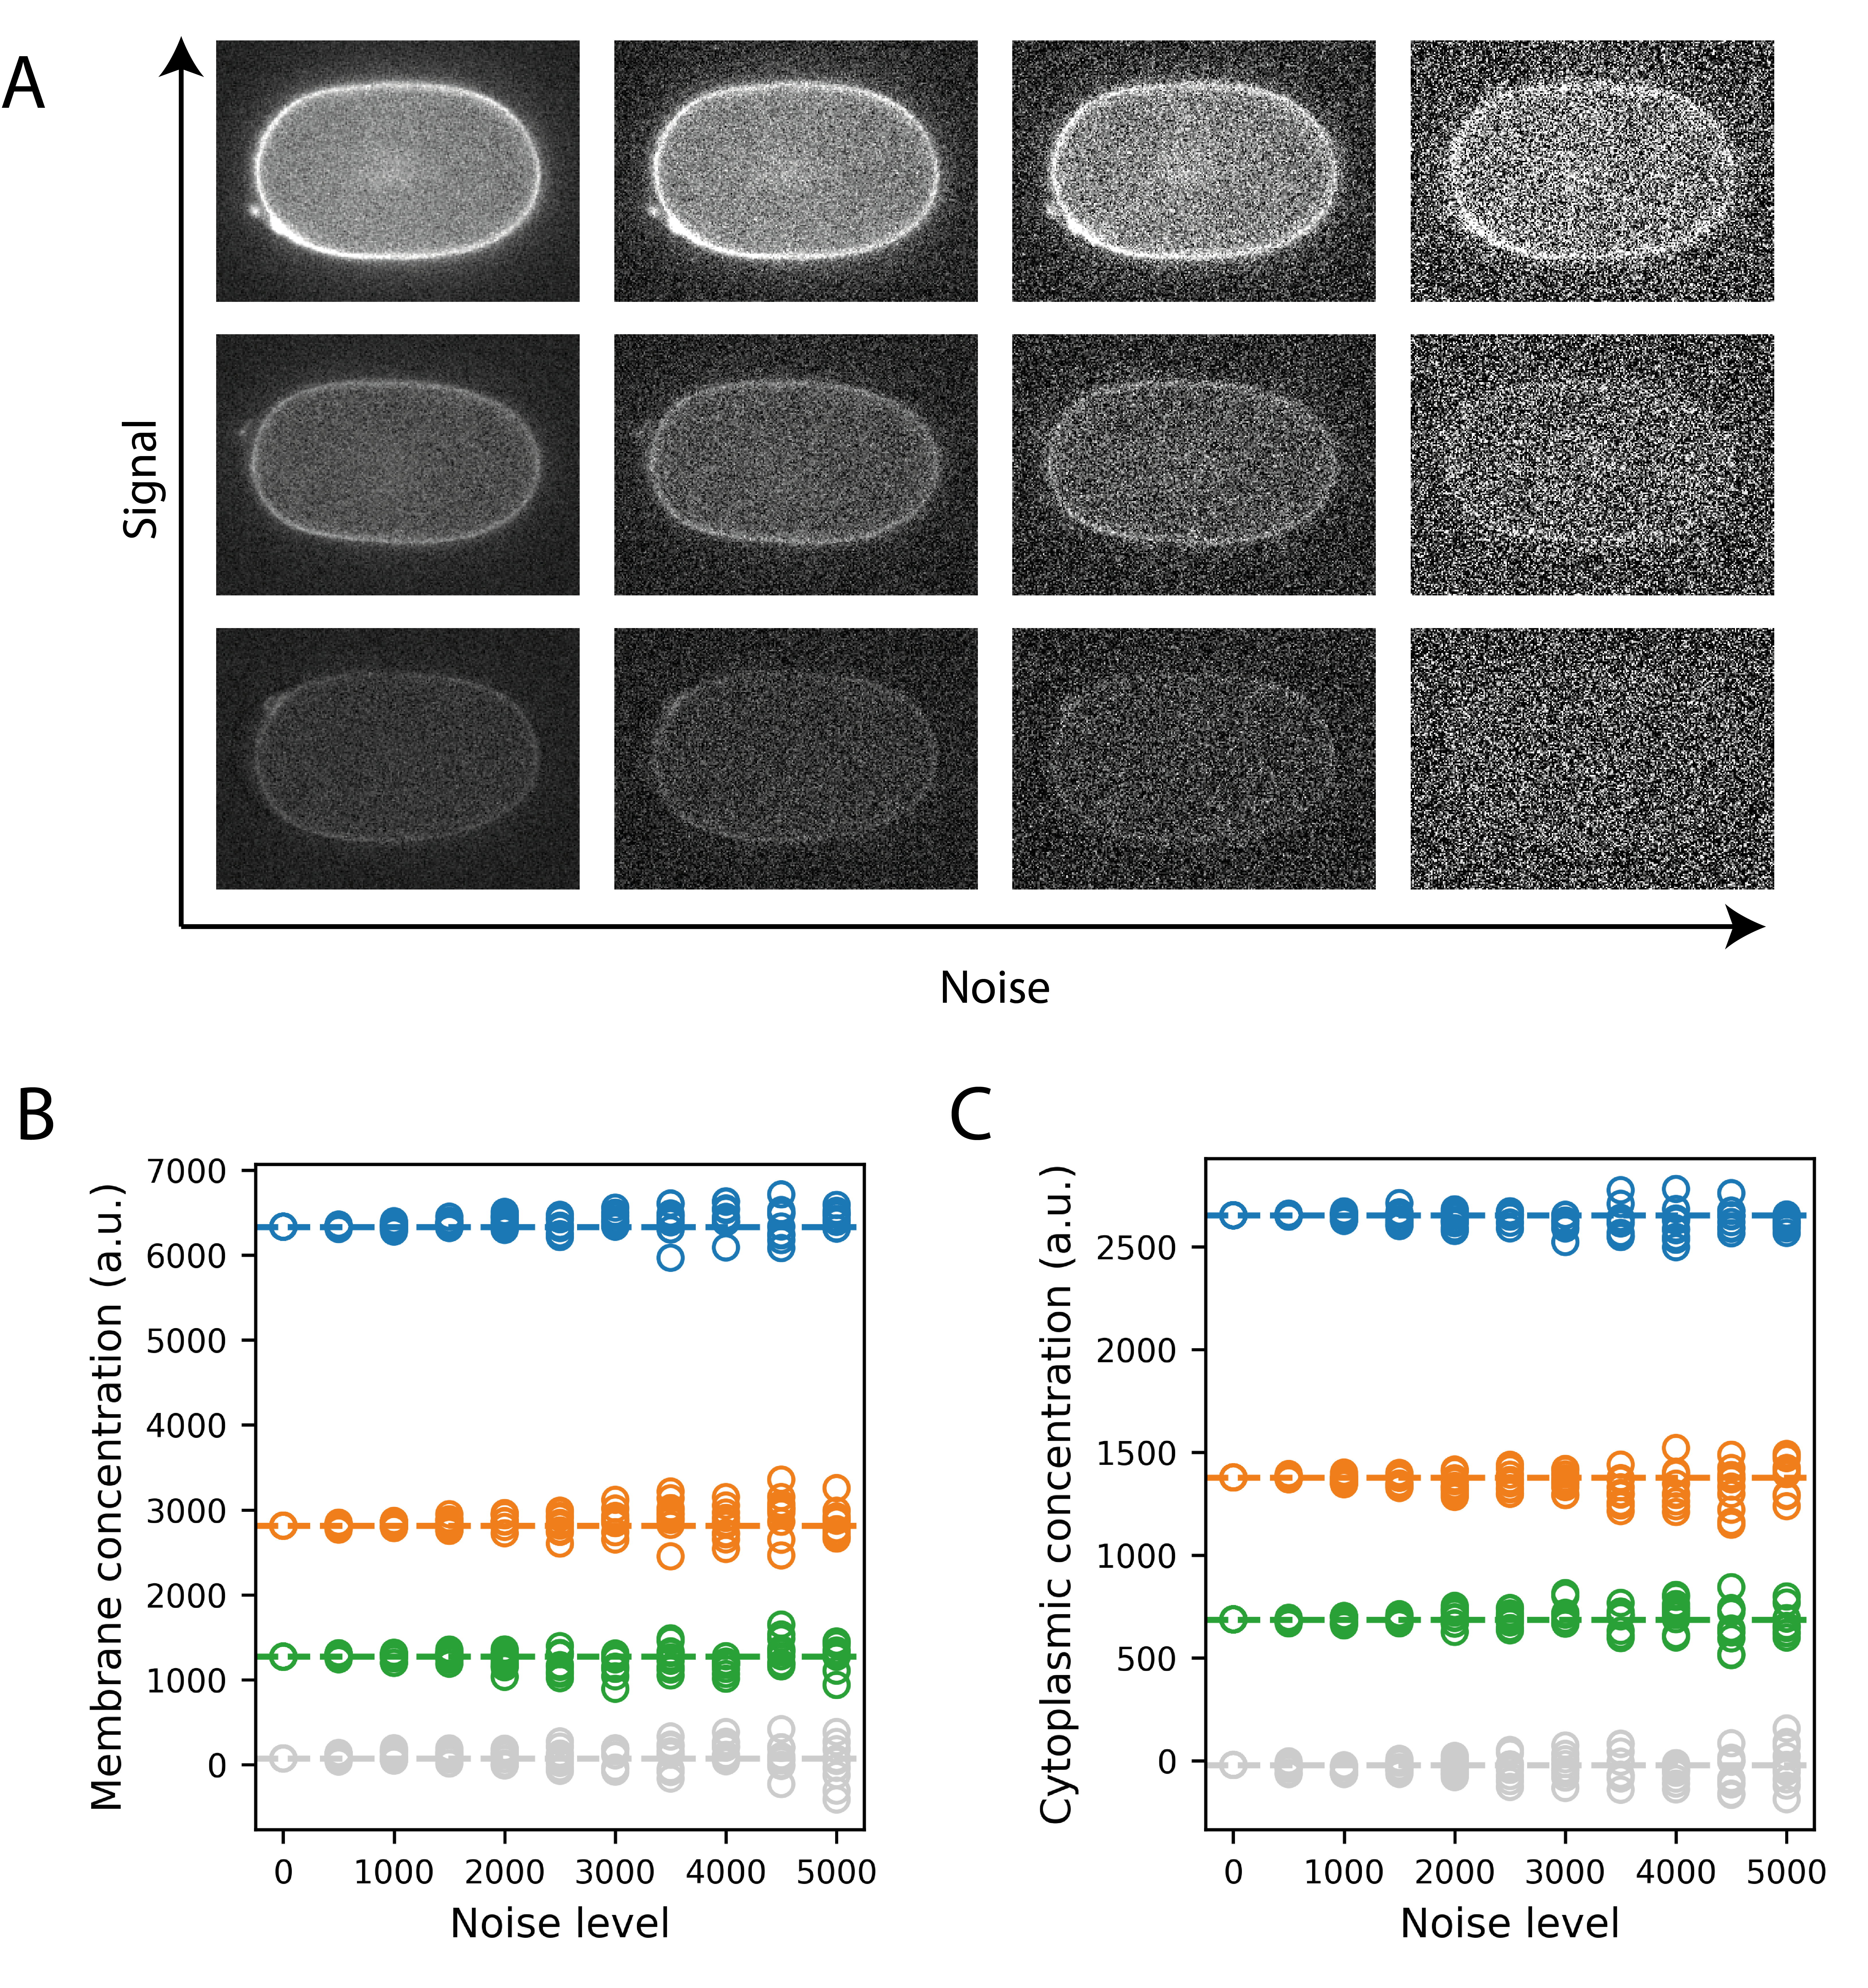
\includegraphics[scale=0.95]{memquant_benchmarking_noise}
\centering
\mycaption{Quantifications of membrane and cytoplasmic concentrations are robust to pixel-noise}{
\textbf{(A)} Images of three GFP::PH expressing embryos with varying amounts of GFP::PH subject to varying levels of Gaussian pixel noise.
\textbf{(B)} Quantifications of membrane concentration (averaged over the entire embryo) for the three embryos in (A) subject to varying levels of pixel noise, colour coded by embryo. For each noise level 10 images were generated for each embryo, and each images was quantified and plot as a single point. Similar analysis for an untagged N2 embryo is also shown (gray). Dashed lines indicate quantification at noise=0.
\textbf{(C)} Quantifications of cytoplasmic concentration for the three embryos in (A) and a single N2 embryo subject to varying levels of pixel noise. Procedure as in (B). Noise level defined as standard deviation of Gaussian noise added to the image. 
}
\label{fig:memquant_benchmarking_noise}
\end{figure}


\subsection{Calibrating concentration units}

As $M$ and $C$ are in arbitrary units (effectively in units of their own respective reference profiles), a conversion parameter is required to put them into common units. To calibrate this conversion parameter, I quantified the effects on $M$ and $C$ measurements of redistributing a fixed pool of protein from the cytoplasm to the membrane. To do this, I used an optogenetics system with a plasma membrane bound PH::eGFP::LOV to move a cytoplasmic pool of ePDZ::mCherry to the membrane (Fielmich et al., 2018). Embryos were exposed to blue light for 10 seconds, which promotes binding between ePDZ and LOV, leading to a rapid uniform recruitment of ePDZ::mCherry to the membrane and a reduction in the cytoplasmic concentration (\cref{fig:memquant_optogenetics}). Where ePDZ::mCherry is expressed alone, this localisation shift is not observed (\cref{fig:memquant_optogenetics}, grey points).\\

\begin{figure}
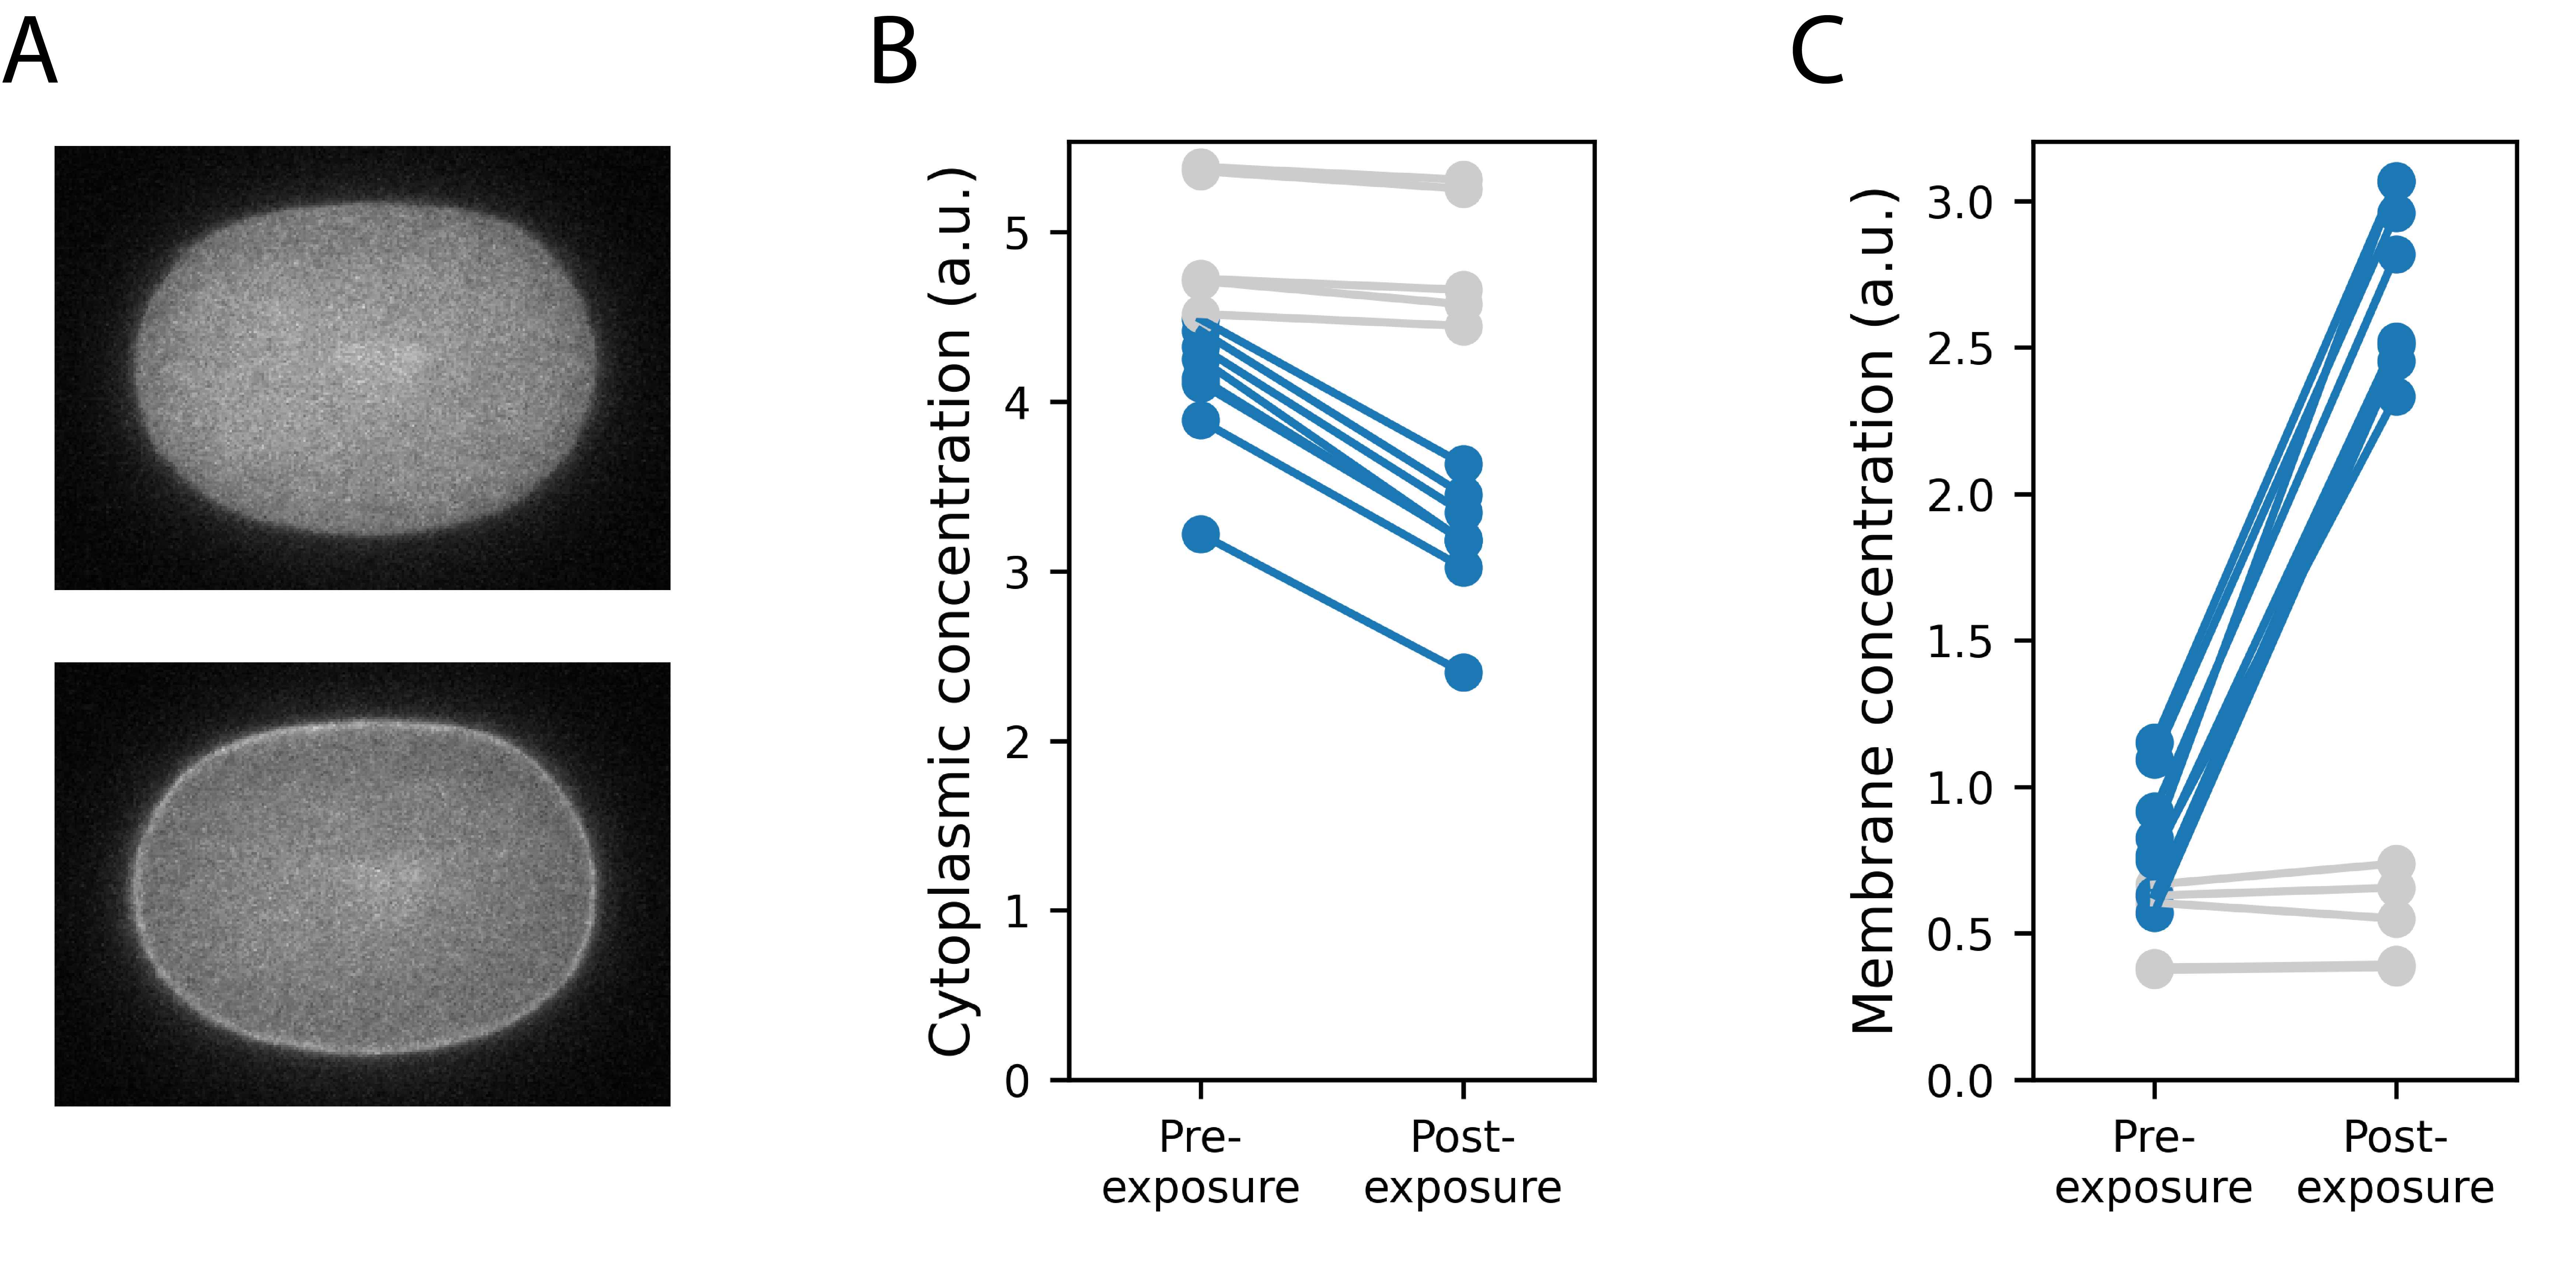
\includegraphics[scale=1]{memquant_optogenetics}
\centering
\mycaption{Redistribution of fluorescent signal from cytoplasm to membrane using optogenetics}{
\textbf{(A)} ePDZ::mCherry before (top) and after (bottom) exposure to blue light, in an embryo also expressing PH::eGFP::LOV.
\textbf{(B)} Cytoplasmic concentration of ePDZ::mCherry (in arbitrary units) before and after blue light exposure for embryos with (blue) and without (gray) PH::eGFP::LOV. 
\textbf{(C)} Membrane concentration of ePDZ::mCherry (in arbitrary units) before and after blue light exposure for embryos with (blue) and without (gray) PH::eGFP::LOV. 
}
\label{fig:memquant_optogenetics}
\end{figure}

Whilst there is significant protein relocalisation in the optogenetic system, the total amount of protein before and after blue light exposure can be assumed to be constant. This total amount, $T$, can be expressed as the $C$ value that would be expected if all tagged molecules were in the cytoplasm, given by equation \ref{eq:t} where $\psi$ is the surface-area to volume ratio of the cell ($= 0.174 \mu m ^ {-1}$ \citep{Goehring2011a}). Given that $M$ is in different arbitrary units to $C$, a conversion parameter, $c$, is required:

\begin{equation}
T = C + \psi c M
\label{eq:t}
\end{equation}

Given that $T$ is the same before and after exposure, $c$ can be calculated, on an embryo by embryo basis, by comparing the gain in $M$ post-exposure to the loss in $C$:

\begin{equation}
c = \frac{C_{pre \textrm{-} exposure} - C_{post  \textrm{-} exposure}}{\psi (M_{post  \textrm{-} exposure} - M_{pre  \textrm{-} exposure})}
\end{equation}\\

Performing this analysis on the dataset in \cref{fig:memquant_optogenetics} (blue points) gives a value of $c$ = 2.88 $\pm$ 0.12 $\mu$m (mean $\pm$ SD), which can be used to convert membrane concentrations to the same common units as cytoplasmic concentrations (i.e. $\mu m^{-3}$ for cytoplasmic concentrations and $\mu m^{-2}$ for membrane concentrations). Note that these concentrations are still arbitrary in the sense that they do not indicate absolute concentrations (i.e. absolute number of molecules per unit area). However, for most of the analysis in the following sections, where the aim is to measure relative concentrations and membrane affinities (membrane to cytoplasmic ratios), this will not be an issue.\\

\clearpage
\subsection{Discussion}

Accurate quantification of features from images relies on the ability to separate overlapping signals and correctly attribute signals to their source. In this section, I have described a two-step pipeline designed for accurate quantification of cytoplasmic and membrane concentrations from midplane images of \textit{C. elegans} zygotes. The first step involves separation of autofluorescence and fluorophore signal, and the second step involves separation of signals from cytoplasmic and membrane protein. The overall pipeline is not specific for any particular microscope, and makes no assumptions about the spectral characteristics of the signal components or the optical properties of the imaging system/sample. Whilst the SAIBR method is not fundamentally tied to \textit{C. elegans}, and has been shown to apply to other systems, the method for separation of cytoplasmic and membrane signals is probably less generalisable, and a number of assumptions in the model presented here are firmly linked to the simple and reproducible geometries of \textit{C. elegans} zygotes and PAR protein patterns. Nevertheless, the method lends great support for the use of differentiable programming for custom quantification of fluorescence images, something that I feel has great potential in a number of applications.\\

Overall, the ability to confidently quantify relative membrane and cytoplasmic concentrations in vivo brings forward new experimental possibilities for studies of the \textit{C. elegans} PAR network, and will prove fundamental to much of the work presented in the following chapters of this thesis.\\


%%%%%%%%%%%%%%%%%%%%%%%%%%%%%%%%%%%%%%%%%%%%%%%%%%%%%%%%%%
\clearpage
\chapter{Uncovering a PAR-2 positive feedback circuit}

\textbf{Detailed contributions:}\\

The CRISPR mutant alleles used in this section were constructed by Nisha Hirani. All imaging and analysis was performed by myself.\\

\clearpage
\section{Introduction}

Mutual antagonism, in which aPARs and pPARs exclude each other from the membrane through phosphorylation reactions, is generally understood to be a dominant factor driving self-organisation of PAR polarity. When coupled to a sufficiently strong spatial trigger, such as an advective flow trigger, mutual antagonism alone is sufficient to give rise to stable polarity in mathematical models, provided that the antagonism reactions harbour sufficient nonlinearity. However, a number of experimental observations have been made which cannot be accounted for by such simple models, suggesting that other feedback mechanisms may be important.\\

Of particular interest is PAR-2, a posterior PAR scaffold which recruits the kinase PAR-1. Whilst PAR-2 requires PKC-3 activity to polarise, several observations have been made which appear to violate predictions from mutual antagonism models, and suggest that PAR-2 plays significant roles in polarity formation which are not fully appreciated by existing models.\\

\subsection{The PAR-2 polarity pathway}

As previously discussed, PAR-2 is able to initiate polarity in the absence of cortical flows (`no-flow' conditions) through a localised interaction with microtubules. This interaction protects PAR-2 from phosphorylation by PKC-3, which leads to localised recruitment of PAR-2 to the cortex at the posterior pole \citep{Motegi2011}. Cortical PAR-2 then recruits PAR-1 from the cytoplasm, which antagonises aPARs through phosphorylation of PAR-3.\\

According to a simple mutual antagonism model, if a threshold concentration of pPAR is reached in the posterior, self-organisation can be initiated, resulting in the formation of a normal polarised PAR pattern (\cref{fig:no_flow_sb_model}).\\

% Add something here about Nelio's data?

\begin{figure}
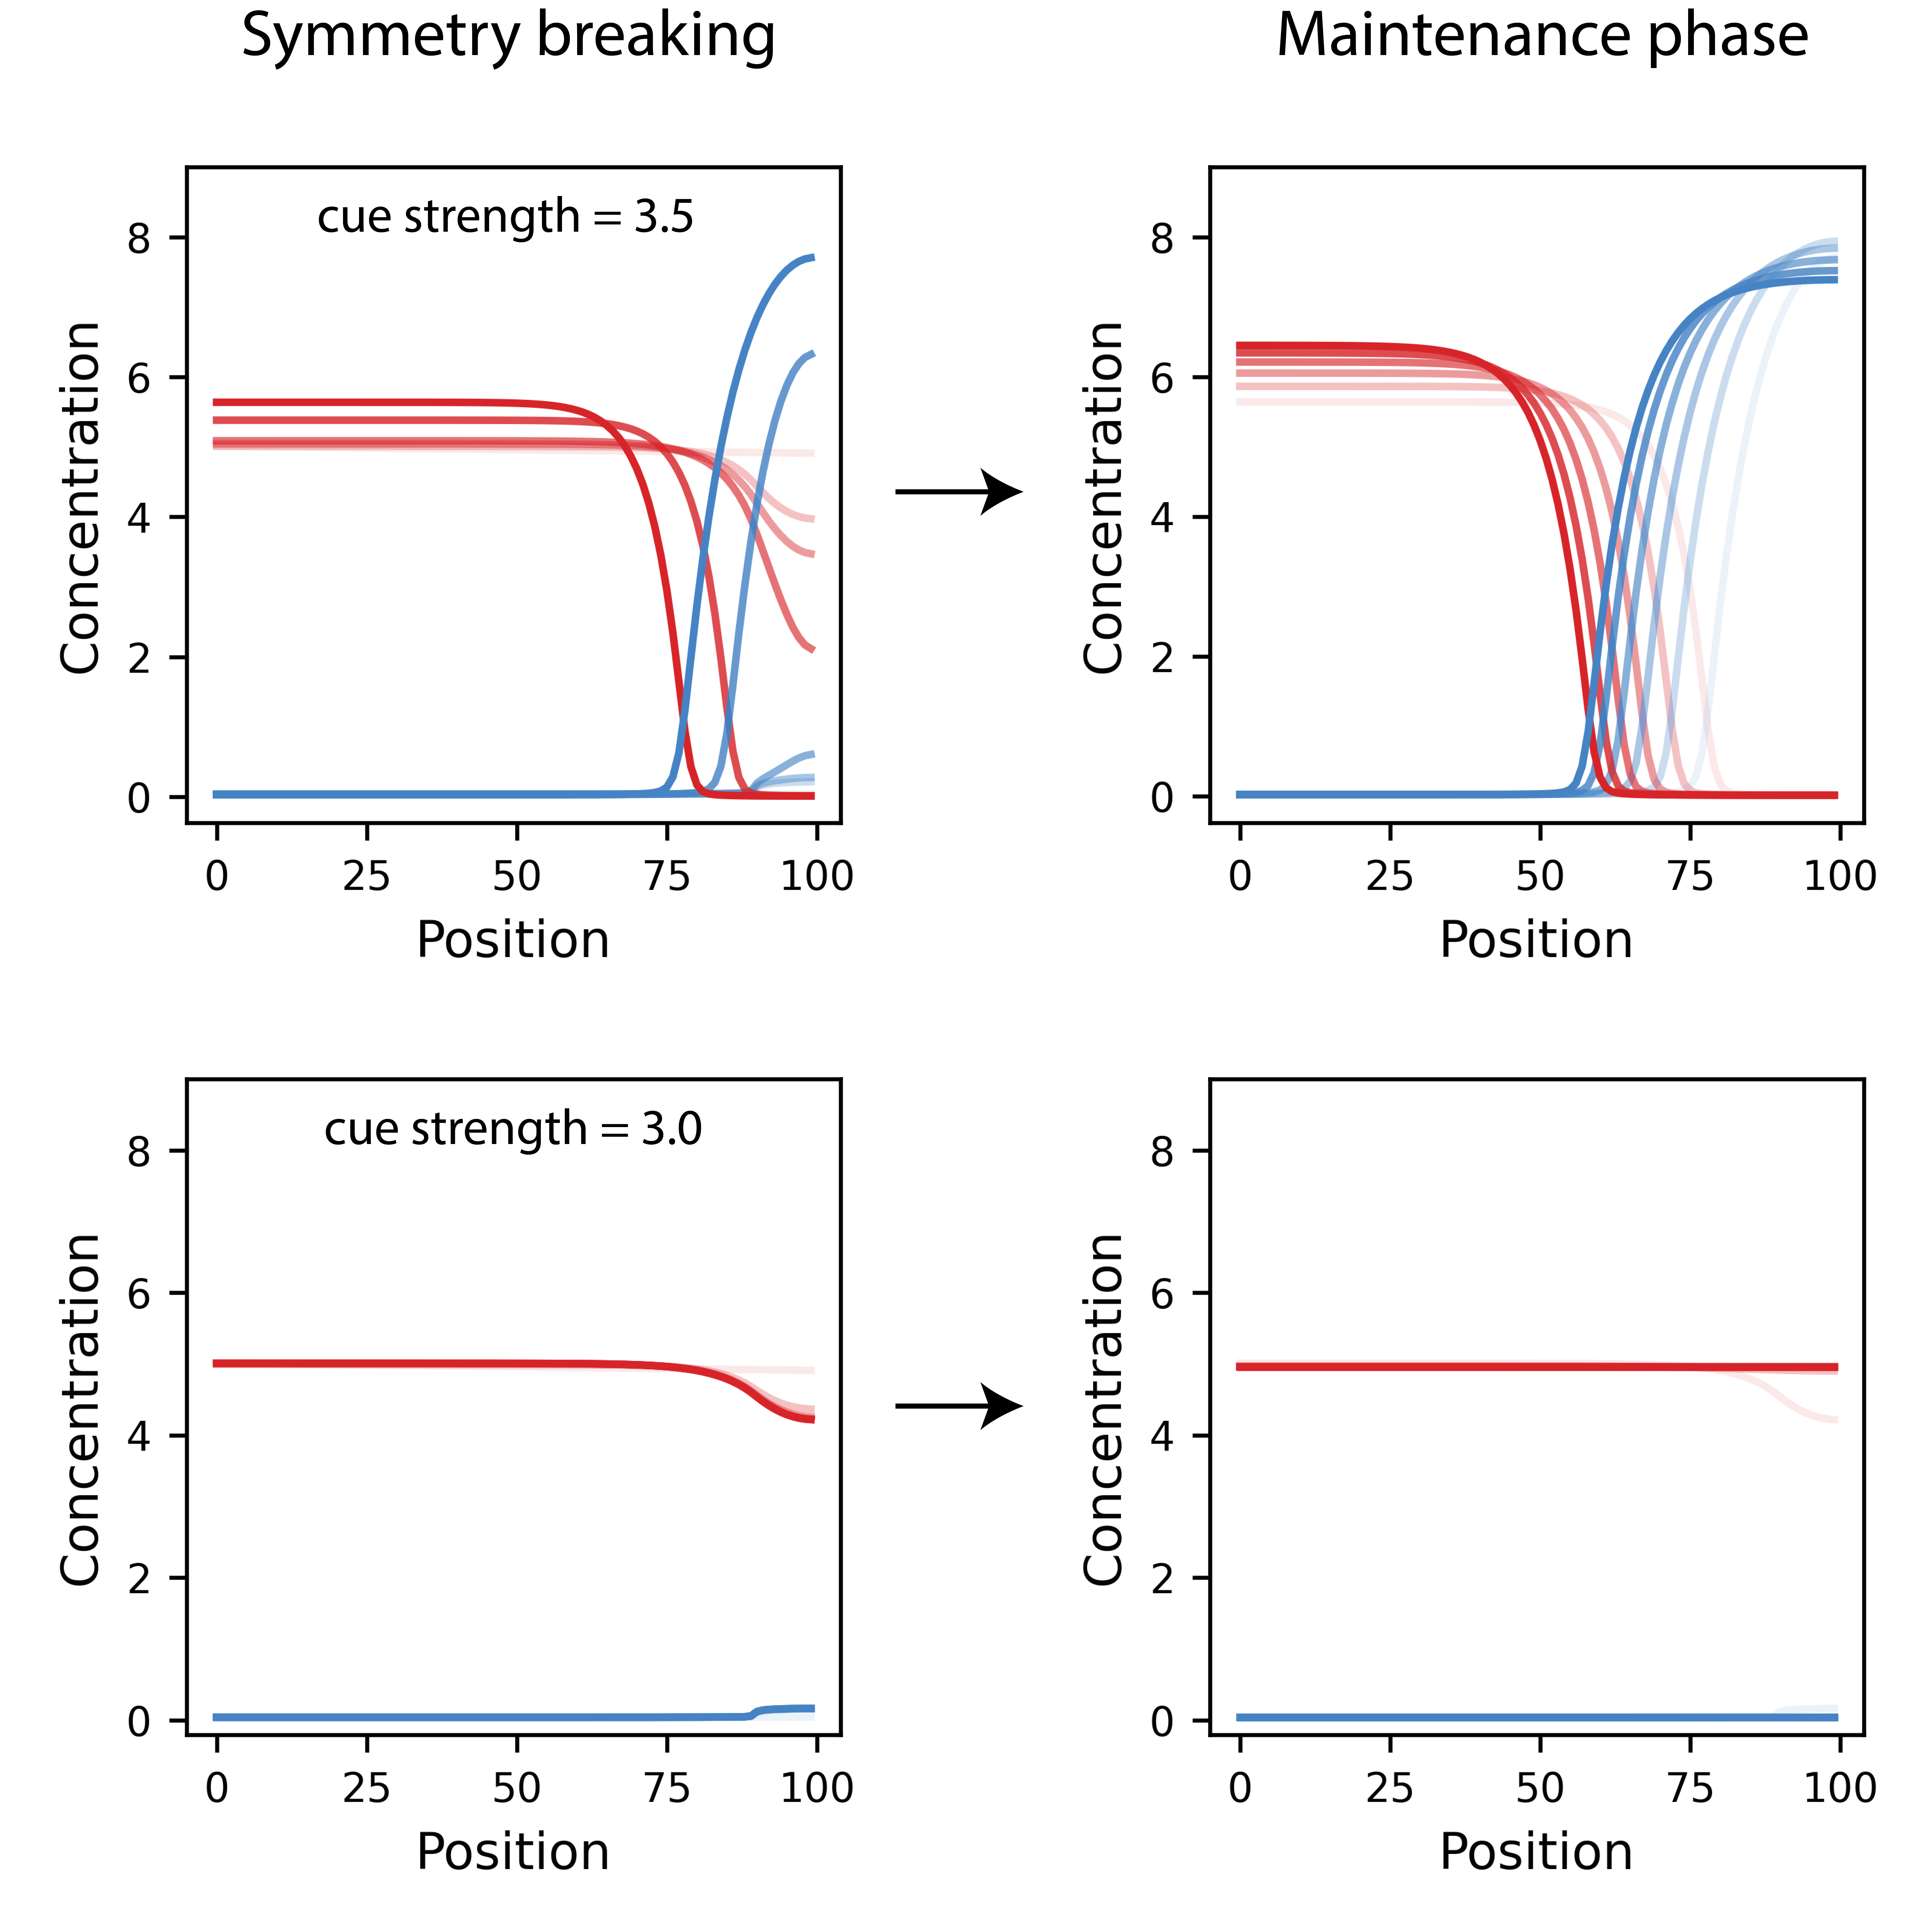
\includegraphics[scale=0.9]{no_flow_sb_model}
\centering
\mycaption{Simulating PAR polarity driven by the microtubule cue}{
Using the minimal PAR model presented in chapter 1, systems were simulated for 1000s with a posterior cue, modelled as a decrease in the antagonism rate from A to P in the posterior 10\% (Symmetry breaking), and then simulated for a further 1000s without a spatial cue (Maintenance phase). Cue strength represents fold change in the antagonism rate from A to P in the posterior 10\%. If the cue is sufficiently strong, a threshold pPAR concentration can be reached in the posterior to initiate self-organisation (top row).}
\label{fig:no_flow_sb_model}
\end{figure}

% Could go into a bit more detail here and show that threshold cue strength depends on off rate, as this would help explain the RING phenotype and might give more weight to the argument that the membrane affinity of the microtubule mutants may be significant

Strikingly, and in contrast to predictions from the mutual antagonism model, it has been shown that formation of a stable PAR-2 domain in these conditions does not actually require aPARs to be cleared from the posterior cortex \citep{Motegi2011}. In \textit{par-1} mutant conditions, or with a \textit{par-3} mutant lacking the PAR-1 phosphorylation site (S950A), PAR-2 domains are able to be initiated, and spread, without corresponding clearance of aPARs, leading to spatial overlap of aPARs and pPARs in the posterior. The fact that PAR-2 can polarise without spatial information from the aPARs implies that additional positive feedback mechanisms must exist that contribute to PAR-2 polarity (\cref{fig:polarity_regimes_schematics}). Specifically, the fact that PAR-2 domains can overlap with PKC-3 implies that feedback mechanisms must exists that allow cortically enriched PAR-2 to resist or counteract antagonism from PKC-3 in the posterior. Here, I will discuss three non-exclusive mechanisms suggested by prior works that could play a role in promoting PAR-2 domain formation under such conditions: 1) self-recruitment, 2) RING domain activity, 3) PKC-3/PAR-2 interactions.\\


\begin{figure}
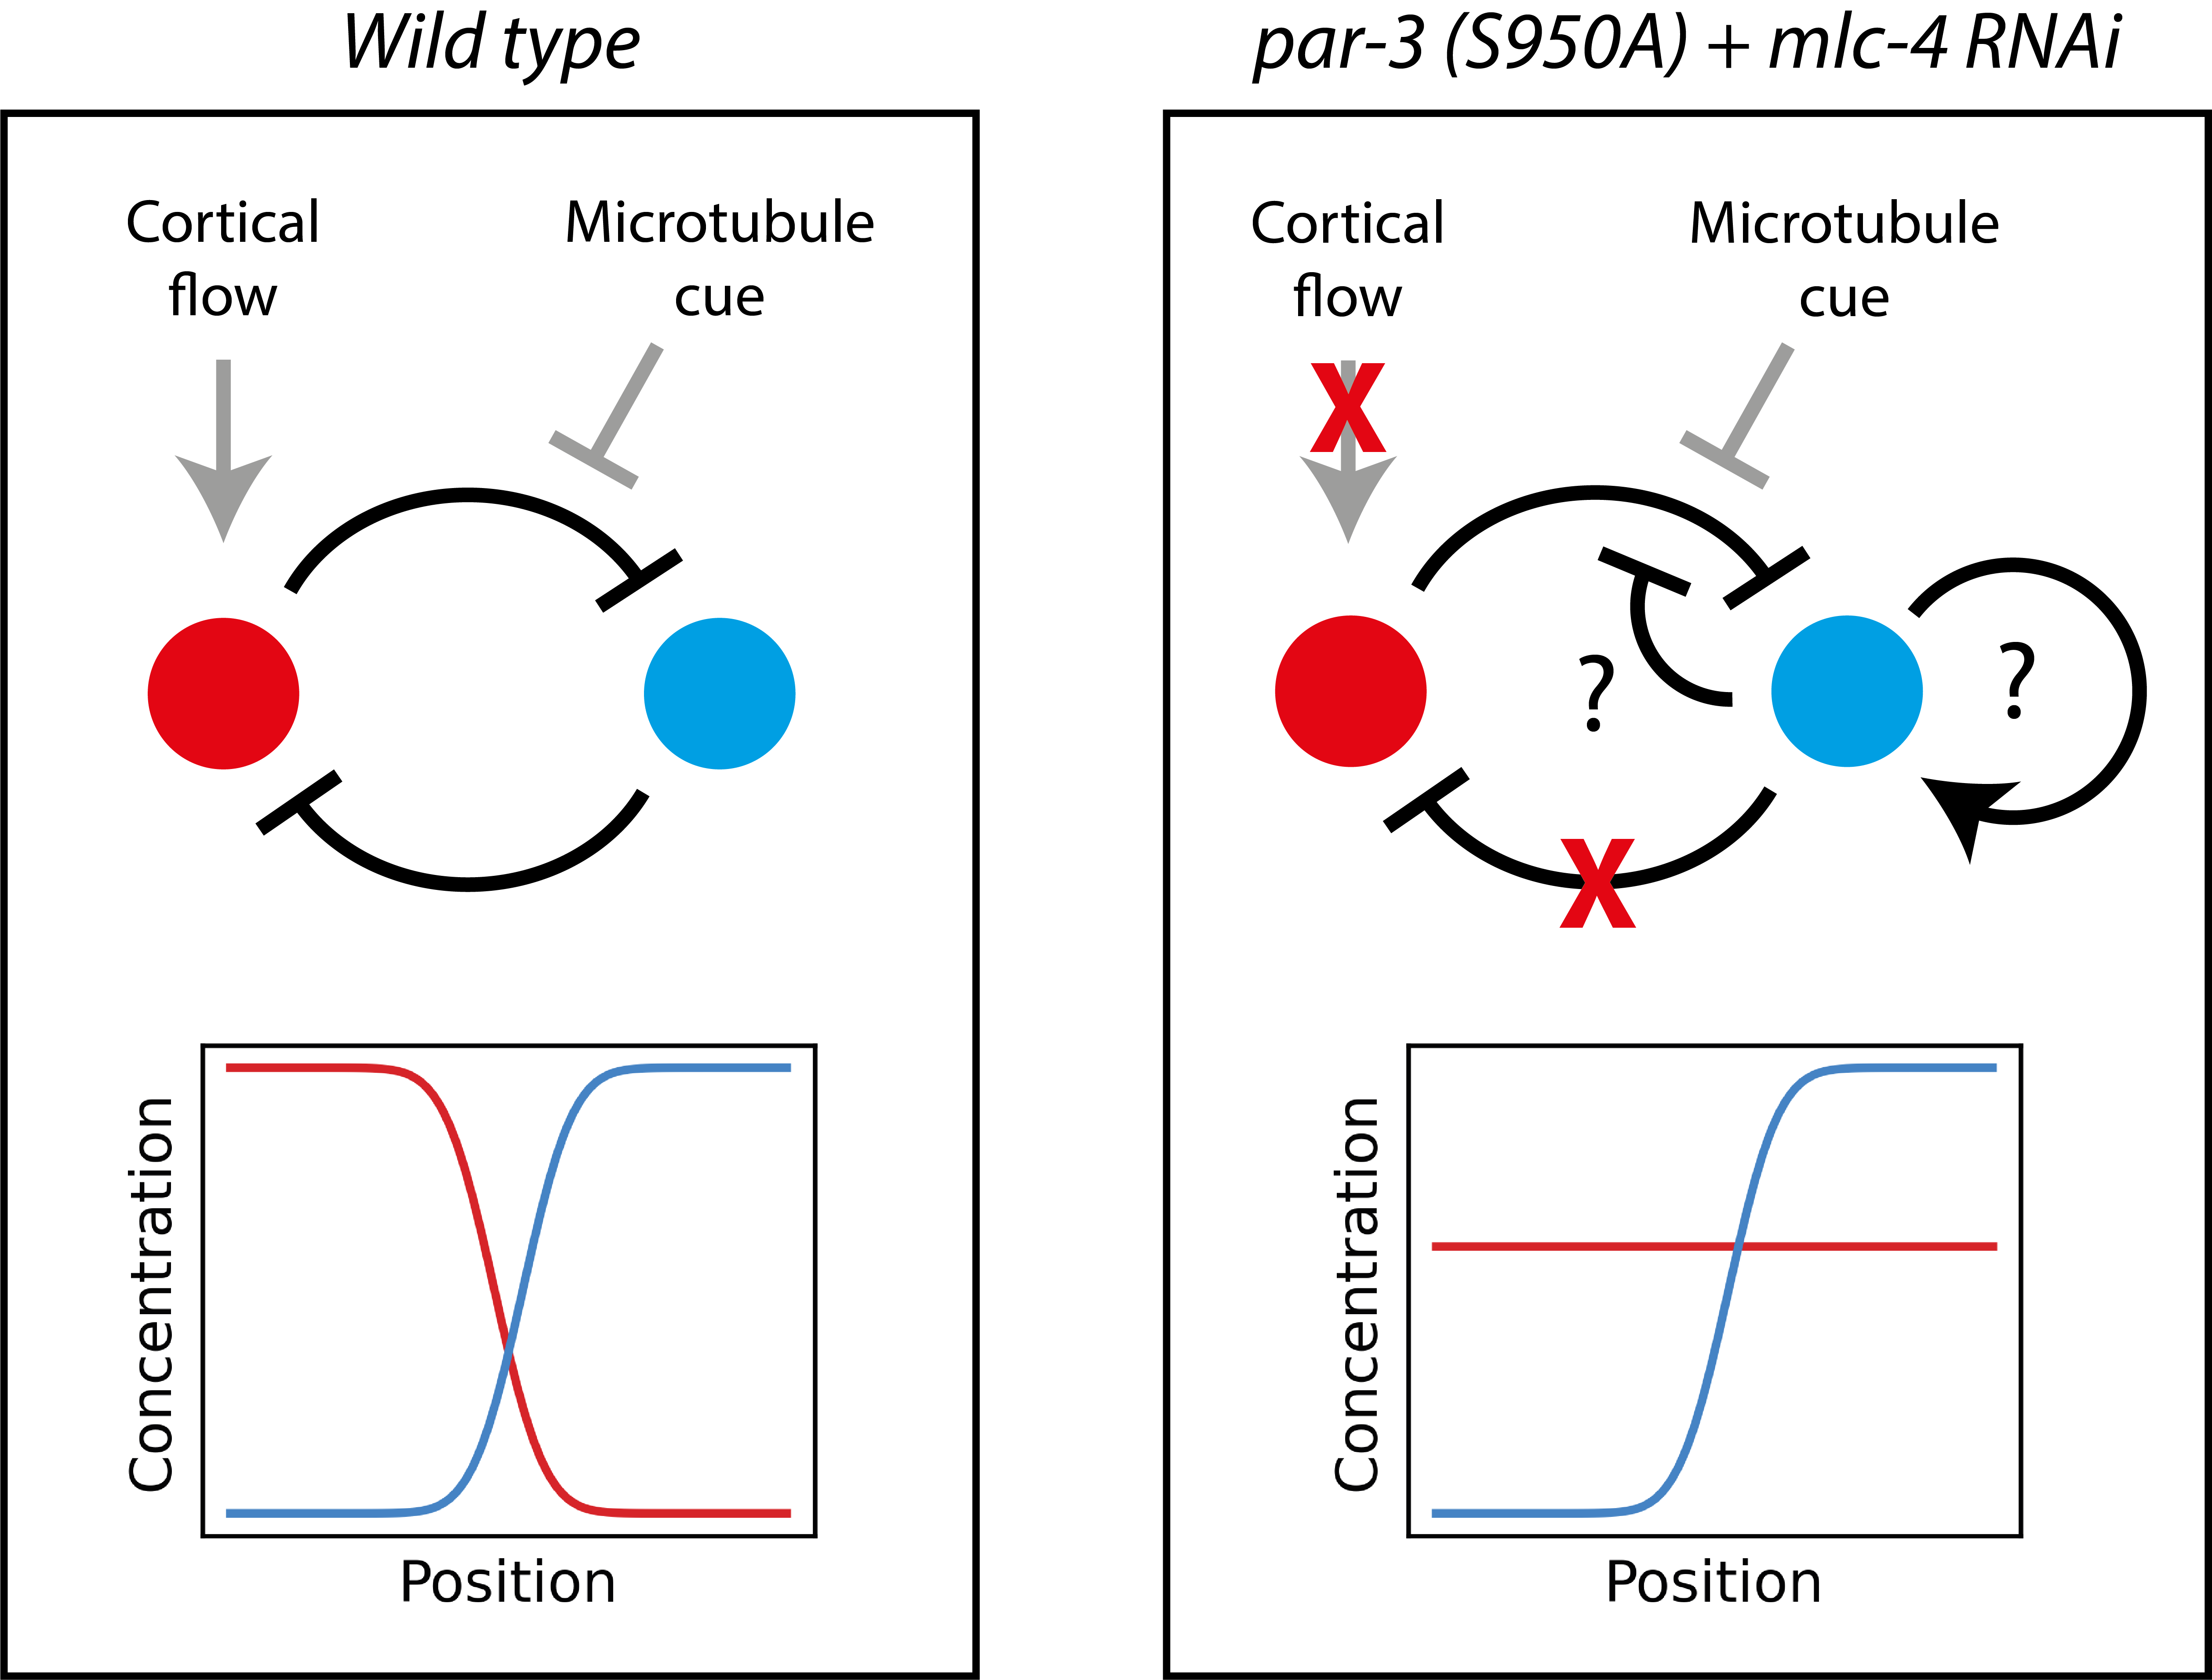
\includegraphics[scale=1.1]{polarity_regimes_schematics}
\centering
\mycaption{Schematic of pPAR polarity in systems with uniform aPAR}{
In systems lacking cortical flows (e.g. \textit{mlc-4 RNAi}) and lacking pPAR to aPAR feedback (e.g. \textit{par-3 (S950A), par-1 RNAi}), aPARs fail to polarise. Nevertheless, PAR-2 is still able to polarise under these conditions, implying the existence of additional feedback reactions. Possible reactions that have been proposed include a positive feedback reaction in which cortical PAR-2 can self-recruit cytoplasmic PAR-2, an inhibitory reaction from PAR-2 to PKC-3 activity, or entry of PAR-2 into a PKC-3 resistant state. The distribution of other pPARs (LGL-1, CHIN-1) in this state is unknown. Black arrows represent feedback reactions. Spatial cues (grey arrows) are active during symmetry breaking but dissipate during maintenance phase.
}
\label{fig:polarity_regimes_schematics}
\end{figure}


\subsection{Self-recruitment}

Using an in vitro microtubule pelleting assay, along with analysis of truncation mutants, \textcite{Motegi2011} were able to identify the regions of PAR-2 responsible for microtubule binding. Two independent mutations to basic residues within these regions (R163A and R183-5A, \cref{fig:par2_schematic}) were found to reduce the level of microtubule binding in vitro, and prevent symmetry breaking in no-flow conditions in vivo. Interestingly, whilst these mutants are usually unable to access the cortex in conditions with uniform aPAR, they can do so when wild-type PAR-2 is also present. This has led to proposals that PAR-2 may have the ability to self-recruit, meaning that cortical PAR-2 molecules may recruit additional cytoplasmic PAR-2 molecules to the cortex. In line with this, PAR-2 has been shown to weakly self-associate in in vitro pull-down assays \citep{Motegi2011, Arata2016}.\\

\textcite{Arata2016} expanded on this by showing that PAR-2 exists as oligomers at the cortex. By total internal reflection fluorescence (TIRF) imaging, the authors were able to resolve distinct PAR-2 particles of varying size at the cortex (up to tetrameric), which showed a slight asymmetry towards larger oligomers at the posterior. Membrane lifetime was found to vary slightly across the cell according to oligomer size and local PKC-3 concentration, indicating that oligomerisation can increase, and phosphorylation decrease, the stability of membrane binding. However, their observed lifetime asymmetry was small compared to the concentration asymmetry of PAR-2, and so the authors also postulated an asymmetric membrane association rate, highest in the posterior of polarised cells, which they suggest could be due to direct recruitment of cytoplasmic PAR-2 into cortical oligomers.\\

Self-recruitment may lead to a positive feedback reaction, whereby cytoplasmic PAR-2 is preferentially recruited to regions of the cortex with high concentrations of PAR-2. Such a reaction may allow the PAR-2 domain to independently grow and self-stabilise, even in the presence of a uniform antagonist. However, the extent to which this reaction impacts the membrane association behaviour of PAR-2 is not understood, and we lack quantitative data to assess the strength and significance of this feedback. Furthermore, quantitative measurements of oligomerisation affinity and oligomer size using biophysical methods have not been performed, and the mechanism of this proposed oligomerisation reaction is unclear. \\


\subsection{RING domain}

Studies of mutant PAR-2 alleles have demonstrated an important role for the N-terminal RING domain in establishing strong PAR-2 domains. Under normal conditions, a RING mutant PAR-2 (C56S) can form a posterior polarity domain following aPAR advection, but this domain is weakly concentrated compared to wild type PAR-2 \citep{Hao2006}. Following cessation of flows at maintenance phase, aPARs spread back towards the posterior, causing the PAR-2 domain to be largely cleared by the time of cytokinesis. This implies that RING-mutant PAR-2 domain lacks the fundamental properties of wild type PAR-2 domains that allow them to overcome antagonism from PKC-3. In no-flow conditions, PAR-2 C56S remains entirely cytoplasmic and unable to trigger formation of a domain \citep{Motegi2011}. Whilst it is clear that the RING plays a significant role in organising the PAR-2 domain, insight into the mechanisms of RING domain action is lacking. The extent to which the RING phenotype is a consequence of intrinsically lower membrane affinity, failures in the self-recruitment pathway described above, or is due to an as yet undefined function important for resisting PKC-3 displacement (as proposed by \textcite{Hao2006}), is unclear. PAR-2 has been argued to act as a ubiquitin ligase, but no evidence beyond modest yeast 2-hybrid interactions with E2 enzymes \citep{Gudgen2004} has been published.\\

% Studies of mutant PAR-2 alleles have demonstrated an important role for the N-terminal RING domain in establishing strong PAR-2 domains. Mutations to the putative zinc coordinating residues in the RING domain, designed to misfold the domain and render it non-functional, weaken the strength of PAR-2 cortical localisation \citep{Hao2006}. This is accompanied by faster cortical dynamics as revealed by FRAP, indicative of a shorter membrane lifetime \citep{Motegi2011}. Whilst these mutants can form posterior domains at establishment phase (albeit weakly concentrated), they are rapidly cleared by invading aPARs at maintenance phase \citep{Hao2006}.\\


% Studies on RING mutants also shed potential light on the mechanisms of PAR-2 protection. \textcite{Hao2006} showed that RING mutants are unable to be protected by endogenous PAR-2 in PAR-1 mutant conditions in which aPARs become uniform, suggesting that the RING may be required to react to endogenous PAR-2. Whilst unclear at the time of the study, more recent work showing that PAR-2 can oligomerise, as described above, along with a characteristic role of RING domains in oligomerisation, as described below, may shed potential light on this. However, this hypothesis is yet to be formally tested. Intriguingly, however, Motegi showed that in near identical experimental conditions RING mutant PAR-2 can (seemingly) be protected by endogenous PAR-2. The reason behind this discrepancy is unclear.\\


\begin{figure}
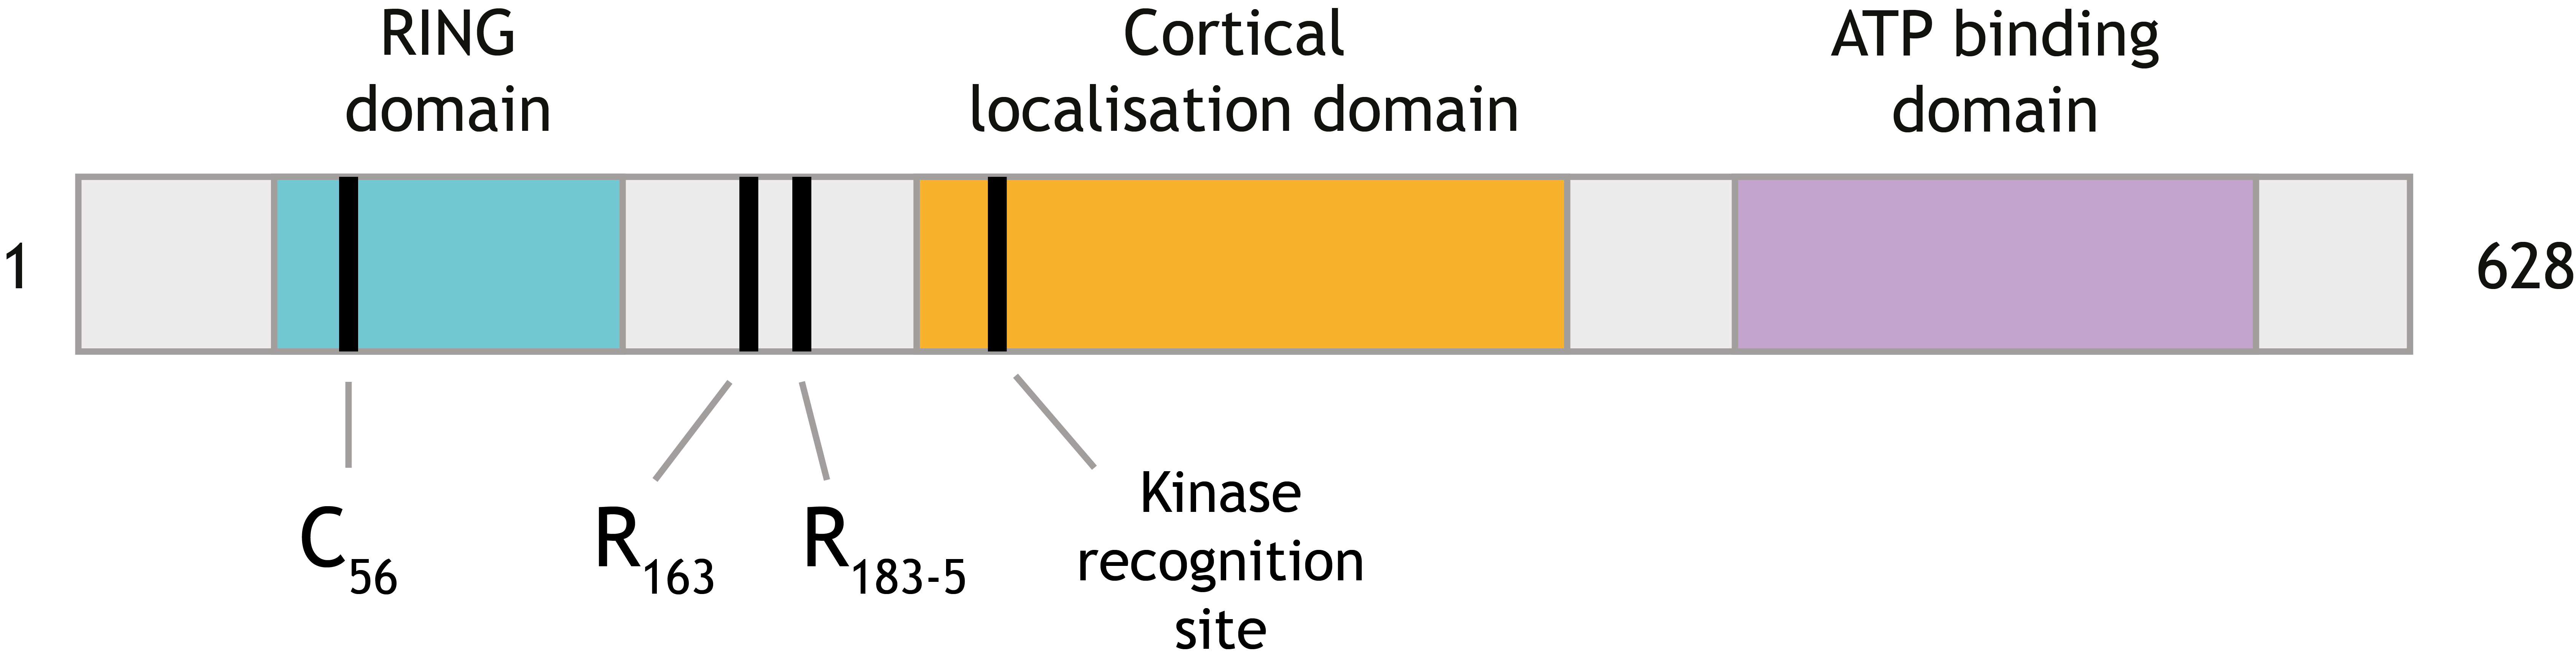
\includegraphics[scale=0.95]{par2_schematic}
\centering
\mycaption{Schematic representation of PAR-2}{
Indicates the position of sites for which mutation disrupts PAR-2 driven polarity in no-flow regimes.
}
\label{fig:par2_schematic}
\end{figure}

\subsection{PKC-3/PAR-2 interactions}

PAR-2 contains an FxR motif, which acts as a high affinity PKC-3 recognition motif \citep{Soriano2016}. Unpublished work by Florent Peglion (Goehring lab) has shown that a mutant PAR-2 allele with a weakened recognition motif (PAR-2(AxA)), whist able to polarise relatively normally in wild type backgrounds, is unable to drive polarity in no-flow conditions. A possible interpretation of this result is that the ability for PAR-2 to resist PKC-3 might, perhaps counterintuitively, rely on tight association between PAR-2 and PKC-3. Whilst intermediate substrate affinity is often compatible with efficient enzymatic activity, high substrate affinity can lead to a stable interaction between kinase and substrate which can effectively block enzymatic activity. PAR-3, which has a similar PKC-3 recognition site to PAR-2, can act as either a substrate or an inhibitor of PKC-3 depending on its affinity, which is under regulatory control \citep{Soriano2016}. In the case of PAR-2, regulation of binding affinity to PKC-3, perhaps via nonlinear concentration-dependent behaviours, may underlie its ability to resist antagonism in some contexts, whilst being sensitive in other contexts. Work to uncover the nature of the PAR-2/PKC-3 interaction is ongoing in the Goehring lab, and I will discuss this further in appendix 1.\\

\subsection{Outlook}

Overall, this data suggests a more central role for PAR-2 in driving polarity that extends beyond the mutual antagonism model. Whilst under normal conditions, advective transport and mutual antagonism may dominate the patterning process, the secondary microtubule-dependent pathway appears to rely, at least partially, on feedback reactions intrinsic to PAR-2 itself. A rough model has been suggested in which PAR-2 is initially recruited to the cortex by a local interaction with microtubules, and self-recruitment of PAR-2 molecules from the cytoplasm then enhances cortical PAR-2 concentrations. Diffusive spread, along with the ability to resist PKC-3 when highly concentrated could then allow PAR-2 to spread anteriorly and rapidly invade cortical space occupied by aPAR. Once a PAR-2 domain forms, cortical PAR-2 recruits PAR-1 from the cytoplasm. By phosphorylating PAR-3, PAR-1 eventually clears aPARs from the posterior, restricting them to the anterior.\\

This model, however, remains largely speculative as there is little to no direct evidence to support positive feedback or direct antagonism of PKC-3 by PAR-2. Critically for our goals in building quantitative models, there is little rigorous quantitative analysis of various PAR-2 mutants (or even wild type PAR-2) that can be used to inform and distinguish mechanistic models for PAR-2-driven polarity, including membrane affinity, protein levels, or dose-response measurements that are essential to understanding feedback. Recent advances in techniques for in vivo quantification, described in the previous chapter, overcome some of these barriers and should enhance our ability to obtain accurate quantitative data. \\

Additionally, previous studies are complicated by their reliance on transgenic lines. As expression of PAR-2 transgenes is not under the same regulatory control as endogenous PAR-2, and the location of transgene insertions in the genome varies from line to line, protein levels are often not comparable to endogenous protein levels, and can strongly differ between lines. This is a potential concern, as the ability for PAR-2 to polarise in no-flow conditions is sensitive to small changes in PAR-2 amounts (Rodrigues et al., in prep). Recent advances in CRISPR technologies mean that we can now tag and monitor endogenous PAR-2 with relative ease, which may control for this potentially confounding factor.\\

% Might be worth having a section here where I confirm the phenotypes of the mutants in CRISPR lines (i.e that they can't break symmetry in no-flow). I have a good dataset for the microtubule mutants but not wild type or C56S. Florent has some data for AxA but I would want to redo if its also worth including.

\section{Quantitative characterisation of PAR-2 mutant alleles}

With this in mind, my first aim was to perform quantitative analysis of the membrane association behaviour of PAR-2 and the mutant alleles described previously for which polarity-defective phenotypes have been reported (R163A, R183-5A, AxA and C56S). By CRISPR to an endogenously tagged GFP::PAR-2 line, we created a series of point mutants at the endogenous \textit{par-2} locus (\cref{fig:par2_misc_mutants_quantification}A). In order to separate intrinsic and PKC-3 dependent behaviours, I crossed each line to a line expressing the \textit{par-3 (it71)} allele, a nonsense mutation in which shows no detectable PAR-3 protein in early embryos \citep{Etemad-Moghadam1995}. Consequently, PKC-3 remains cytoplasmic and inactive, and PAR-2 binds uniformly to the cortex (\cref{fig:par2_misc_mutants_quantification}B). Using the protocol described in the chapter 2 involving autofluorescence correction and computational separation of membrane and cytoplasmic signal components, I performed full quantitative analysis of each line. In \cref{fig:par2_misc_mutants_quantification}C and D I present quantifications of membrane to cytoplasmic ratios, a measure of membrane affinity. Fig \ref{fig:par2_misc_mutants_detailed_quantification} shows full quantification results, including cytoplasmic concentrations, membrane concentrations and total protein levels.\\

As expected, whilst PAR-2(AxA) behaves differently to wild type PAR-2 in polarised cells, owing to its weaker interaction with PKC-3, membrane affinity in \textit{par-3 (it71)} cells is equal to wild type, suggesting that the mutant harbours no intrinsic defect in membrane association.\\

The membrane affinity of PAR-2(C56S), by contrast, is greatly reduced compared to wild type. This is the case even in \textit{par-3 (it71)} mutants, suggesting that the localisation defect is, at least partially, intrinsic to PAR-2, rather than via hypersensitivity to PKC-3 as has previously been suggested \citep{Hao2006}. Overall protein levels are also slightly reduced compared to wild type (\cref{fig:par2_misc_mutants_detailed_quantification}A and D). This is in contrast to previous results using transgenic lines which showed higher levels of PAR-2 RING mutants. The reason for this discrepancy is unclear, but I believe that in this case the small reduction in expression compared to wild type may relate to protein instability caused by unfolding of the RING domain (see chapter 4).\\

Surprisingly, I found that the microtubule-binding mutants (R163A and R183-5A) also have weaker membrane affinities compared to wild type PAR-2. This is independent of aPARs, suggesting a defect intrinsic to PAR-2. Such a defect has previously not been reported in studies using these mutant alleles \citep{Motegi2011, Gross2018}. These mutants also have a mild overexpression phenotype, which differs from previous work using transgenic lines which show the same \citep{Motegi2011} or reduced \citep{Gross2018} levels compared to wild type. As a result, membrane concentrations are similar to wild type concentrations despite the reduction in membrane to cytoplasmic ratio. These results are somewhat unexpected, and may indicate that these variants are defective in more than just microtubule binding.\\

\begin{figure}
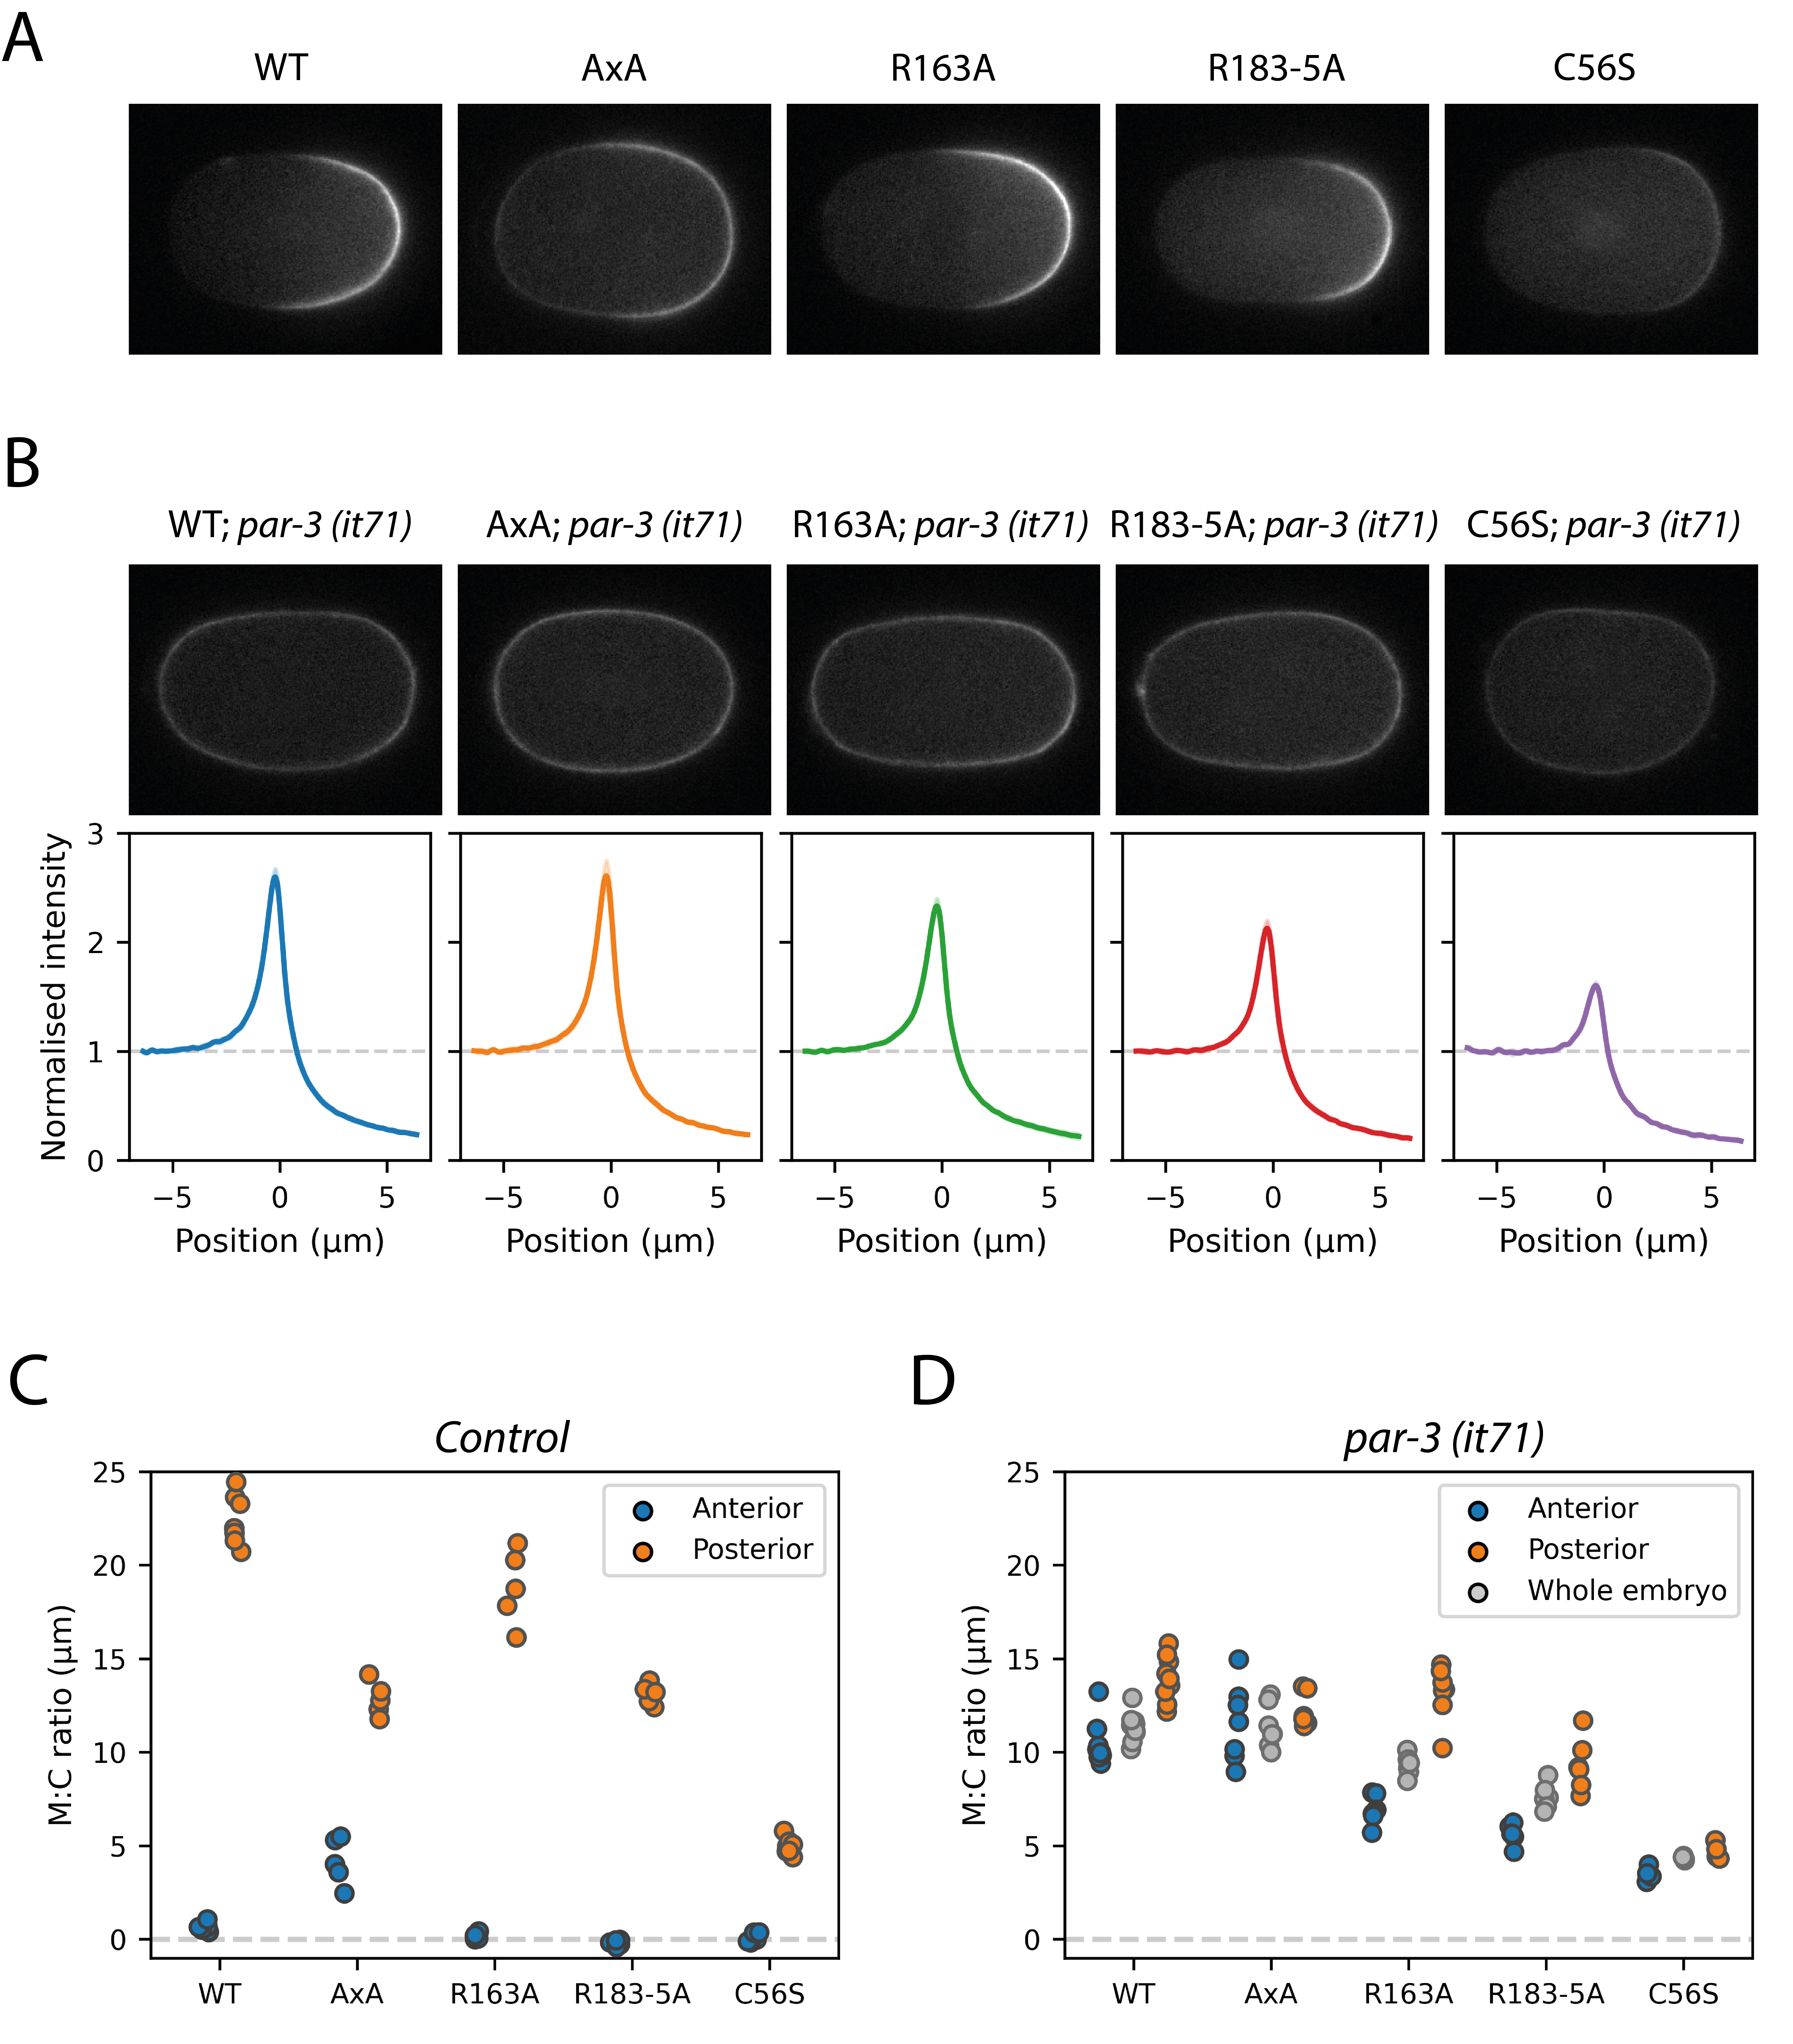
\includegraphics[scale=0.95]{par2_misc_mutants_quantification}
\centering
\mycaption{Membrane affinities of wild-type PAR-2 and mutant alleles in polarised and uniform systems}{
\textbf{(A)} Midplane confocal images of GFP::PAR-2 (wt) and mutant alleles in polarised cells (\textit{par-3 (wt)}) at maintenance phase.
\textbf{(B)} Midplane confocal images of GFP::PAR-2 (wt) and mutant alleles in uniform cells lacking functional aPAR (\textit{par-3 (it71)}). Bottom panels show normalised cross cortex profiles around the entire circumference of the embryo, averaged over all embryos in the dataset (mean $\pm$ SD).
\textbf{(C)} Quantifications of membrane to cytoplasmic ratio for the five PAR-2 alleles in control (\textit{par-3 (wt)}) zygotes. Shows ratios averaged over the anterior and posterior 20\% of the zygote.
\textbf{(D)} Quantifications of membrane to cytoplasmic ratio for the five PAR-2 alleles in uniform (\textit{par-3 (it71)}) zygotes. Shows ratios averaged over the anterior and posterior 20\% of the zygote, and averaged over the whole zygote. All images were taken at NEBD (nuclear-envelope breakdown).
}
\label{fig:par2_misc_mutants_quantification}
\end{figure}

\begin{figure}
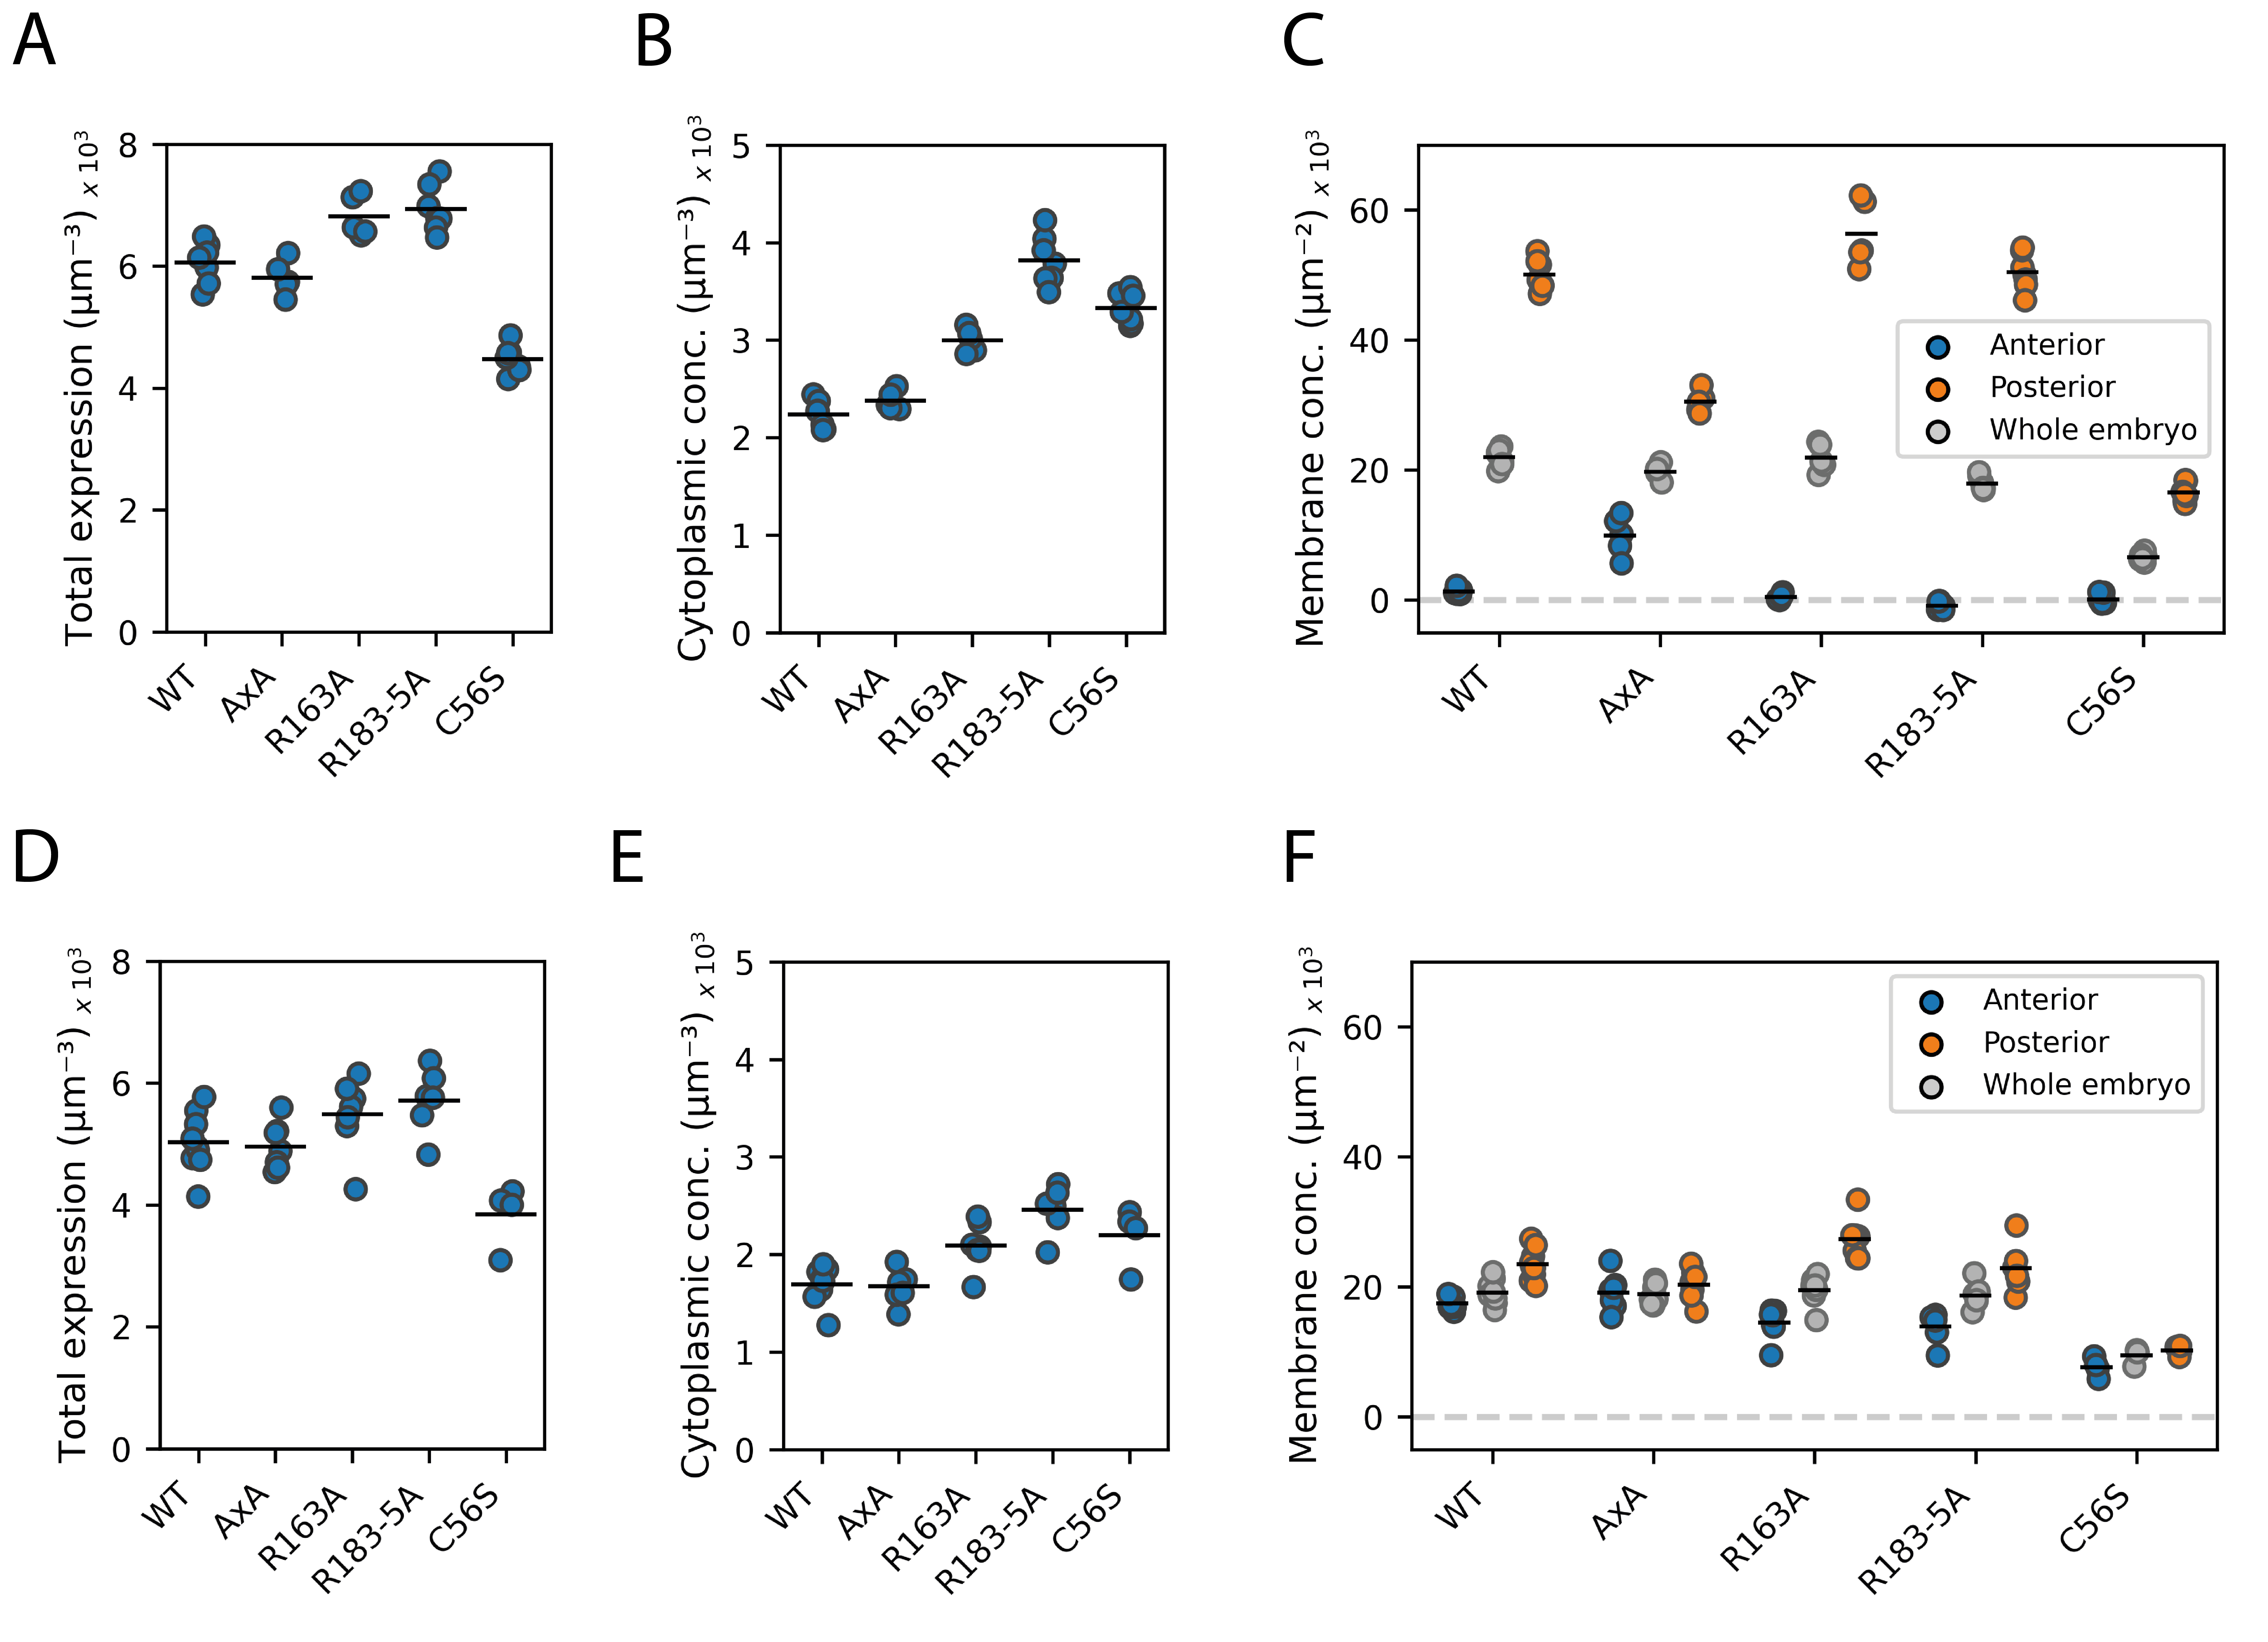
\includegraphics[scale=0.9]{par2_misc_mutants_detailed_quantification}
\centering
\mycaption{Further quantification of wild-type PAR-2 and mutant alleles in polarised and uniform systems}{
\textbf{(A) - (C)} Quantification of total expression (A), cytoplasmic concentration (B) and membrane concentrations (C) for wild type and mutant GFP::PAR-2 in polarised cells (\textit{par-3 (wt)}). 
\textbf{(D) - (F)} Quantification of total expression (D), cytoplasmic concentration (E) and membrane concentrations (F) for wild type and mutant GFP::PAR-2 in uniform cells (\textit{par-3 (it71)}). 
}
\label{fig:par2_misc_mutants_detailed_quantification}
\end{figure}

To summarise, all four mutants presented are defective at polarising in no-flow conditions, consistent with this pathway being highly dependent on PAR-2, although the defects intrinsic to each mutant appear to be quite distinct. The RING domain mutant (C56S) displays a strong and clear membrane binding defect, which may account for its failure to drive polarity via the PAR-2 pathway. PAR-2(R163A) and PAR-2(R183-5A) are defective at binding to microtubules in vitro, and this has previously been understood to underlie their phenotypes in vivo, compatible for a role of microtubules as a polarity trigger. However, my quantification reveals that these mutants also have inherently weaker membrane association, which may provide an additional explanation for their phenotypes. Why this might be is not clear, but it could be that changing the charge profile of the protein (mutating positively charged arginines) affects the electrostatic interaction with the membrane. By contrast, PAR-2(AxA) appears primarily defective in being properly excluded from the anterior by PKC-3, and does not appear to have any intrinsic defects in membrane association. Why this reduction in PKC-3 removal would make it less able to polarise via the PAR-2 pathway is unclear. I investigate the role of the PAR-2 FxR site further in appendix 1.\\


\section{RING domain promotes positive feedback to achieve optimal membrane affinity}
\label{section:par2_rundown}

In examining my data, one additional feature was particularly intriguing. In general, membrane to cytoplasmic ratios were strongly increased in polarised cells compared to uniform cells, the one exception being the RING domain mutant (C56S). In a model that relies solely on mutual antagonism, molecules within their respective domain will generally not be subjected to antagonism, and so the membrane to cytoplasmic ratio of a protein will be set by its intrinsic membrane binding kinetics. Therefore, whilst membrane concentrations may be increased in polarised cells compared to uniform (\textit{par-3 (it71)}) cells due to an increase in the concentration of the cytoplasmic pool, membrane affinity, which is a simple function of membrane binding and unbinding rates, is expected to be constant. In other words, the membrane and cytoplasmic concentrations of a protein undergoing membrane exchange with constant binding and unbinding rates should fall along a linear trajectory (\cref{fig:rundown_schematic}A).\\

However, for wild type PAR-2, this does not appear to be the case, and membrane to cytoplasmic ratios are almost doubled in polarised cells compared to uniform cells (\cref{fig:par2_misc_mutants_quantification} and \ref{fig:par2_misc_mutants_detailed_quantification}). This implies that the rate of membrane association is higher, or the rate of membrane dissociation is lower (or both) in polarised cells compared to uniform cells.\\

Given previous proposals that PAR-2 may be able to self-recruit, I reasoned that such a reaction may be behind this change in kinetics. A positive feedback reaction, whereby PAR-2 promotes its own recruitment to the membrane, may be expected lead to a nonlinear relationship between membrane and cytoplasmic concentrations if feedback is sufficiently strong. The expected shape of the relationship depends on the strength and form of positive feedback. In the simplest case, positive feedback can increase membrane affinity as a function of membrane concentration, such that the gradient of the cytoplasm vs membrane relationship will be higher at higher membrane concentrations (\cref{fig:rundown_schematic}B). Under some parameter regimes, nonlinear feedback may lead to bistability, whereby multiple membrane concentrations can be supported within a range of cytoplasmic concentrations (\cref{fig:rundown_schematic}C). A reaction like this is, in theory, sufficient for polarity in the absence of any additional spatial information, and has been proposed for models involving Rho-GTPases in yeast (e.g. the wave-pinning model \citep{Mori2008}).\\

\begin{figure}[!h]
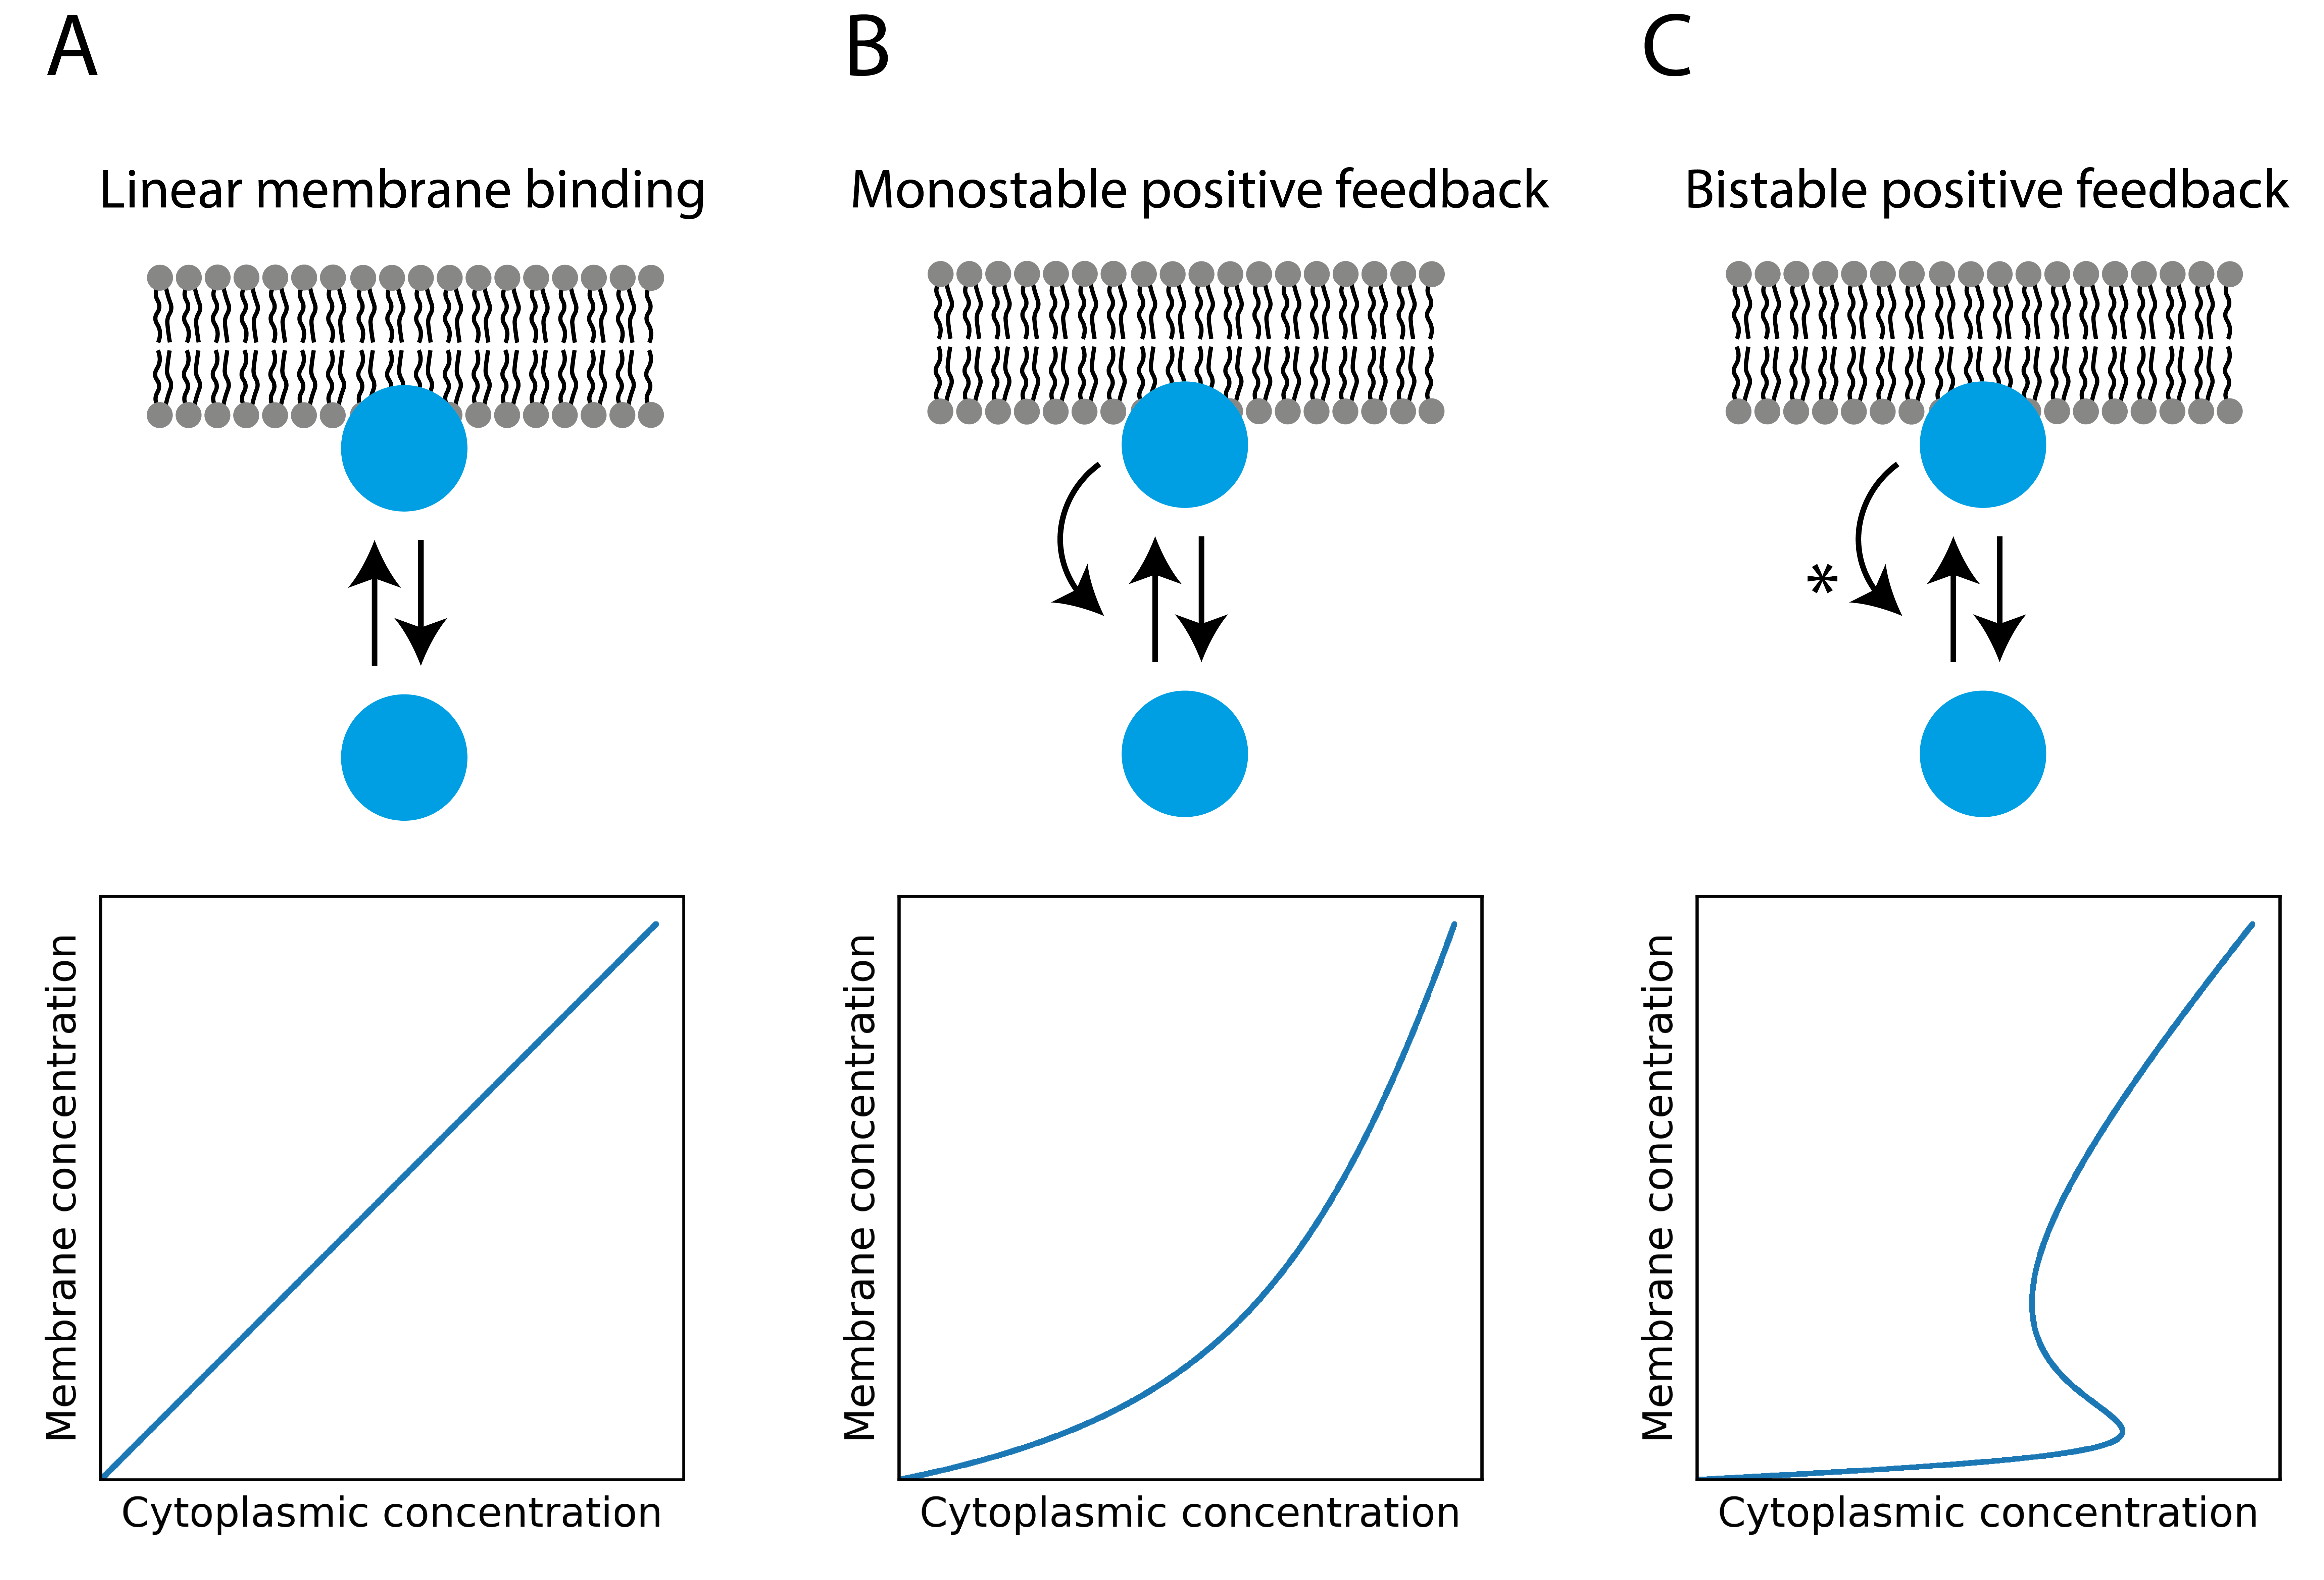
\includegraphics[scale=0.95]{rundown_schematic}
\setlength{\abovecaptionskip}{20pt}
\centering
\mycaption{Cytoplasm versus membrane relationships for models with and without positive feedback}{
A protein exchanging between the membrane and cytoplasm with constant on and off rate kinetics is expected to show a linear relationship between cytoplasmic and membrane concentrations (A).
A protein feeding back onto its own membrane recruitment is expected to have a nonlinear relationship (B).
Where feedback is nonlinearly dependent on membrane concentrations (asterix), bistability can exist under some parameter regimes, whereby multiple membrane concentrations can be supported within a range of cytoplasmic concentrations (C).
ODEs were build using a constant off rate term ($k_{off} = 1$), with on rates specified by the following terms for the three models: (A) $k_1$ (B) $k_2 + \frac{k_3 M}{k_4 + M} $ (C) $k_5 + \frac{k_6 M^2}{k_7^2 + M^2}$ where $k_1 = 1$, $k_2 = 0.05$, $k_3 = 1$, $k_4 = 1$, $k_5 = 0.05$, $k_6 = 1$, $k_7 = 1$ and $M$ is the membrane concentration, and solved for membrane and cytoplasmic concentrations at steady state. 
}
\label{fig:rundown_schematic}
\end{figure}

In a \textit{par-3 (it71)} background, a PAR-2 intrinsic positive feedback reaction implies that the membrane to cytoplasmic ratio should vary with concentration. A commonly used method that can be used to vary protein amounts in \textit{C. elegans} is RNAi, which reduces protein amounts in a manner that can be tuned by duration of dsRNA exposure. To test for the existence of PAR-2 intrinsic positive feedback, I performed an in vivo titration assay using \textit{par-3 (it71)} mutant worms expressing mNG::PAR-2 (wt), in which I used RNAi to rundown protein levels, and quantified membrane and cytoplasmic concentrations on an embryo-by-embryo basis. mNG (NeonGreen) was selected as a fluorophore as it is significantly brighter that GFP, which aids quantification in cells with long RNAi exposures.\\

Strikingly, the results reveal that PAR-2 does not follow strict linear membrane binding kinetics (\cref{fig:rundown_vs_c56s}A, C, D (blue)).  Instead,  a nonlinearity appears to be present, whereby membrane affinities are higher in cells with higher dosages. Whereas the membrane vs cytoplasm relationship for PH (shown previously in fig x) has an effective exponent close to 1,  implying linear mass-action kinetics, the PAR-2 relationship has an exponent of ~2.5, implying cooperative membrane association (\cref{fig:rundown_schematic}D). Notably, however, there is no evidence for any discontinuities that would imply bistable behaviour.\\

Interestingly, unlike wild type PAR-2, the membrane affinity of PAR-2 (C56S) is equal in polarised and \textit{par-3 (it71)} systems, despite large changes in membrane and cytoplasmic concentrations. This suggests that the mechanism of positive feedback may be RING-dependent. To test this, I performed a similar titration assay using the PAR-2 (C56S) mutant line. The results (\cref{fig:rundown_vs_c56s}B, C, D (orange)) show that the nonlinearity of the cytoplasm vs membrane relationship is greatly reduced compared to wild type, implying that the RING domain plays an essential role in promoting positive feedback.\\

% Some degree of nonlinearity appears to be maintained (exponent ~ 1.7). This might imply that some non-RING-dependent mechainsms contribute to nonlinear membrane association. More...


\begin{figure}[!h]
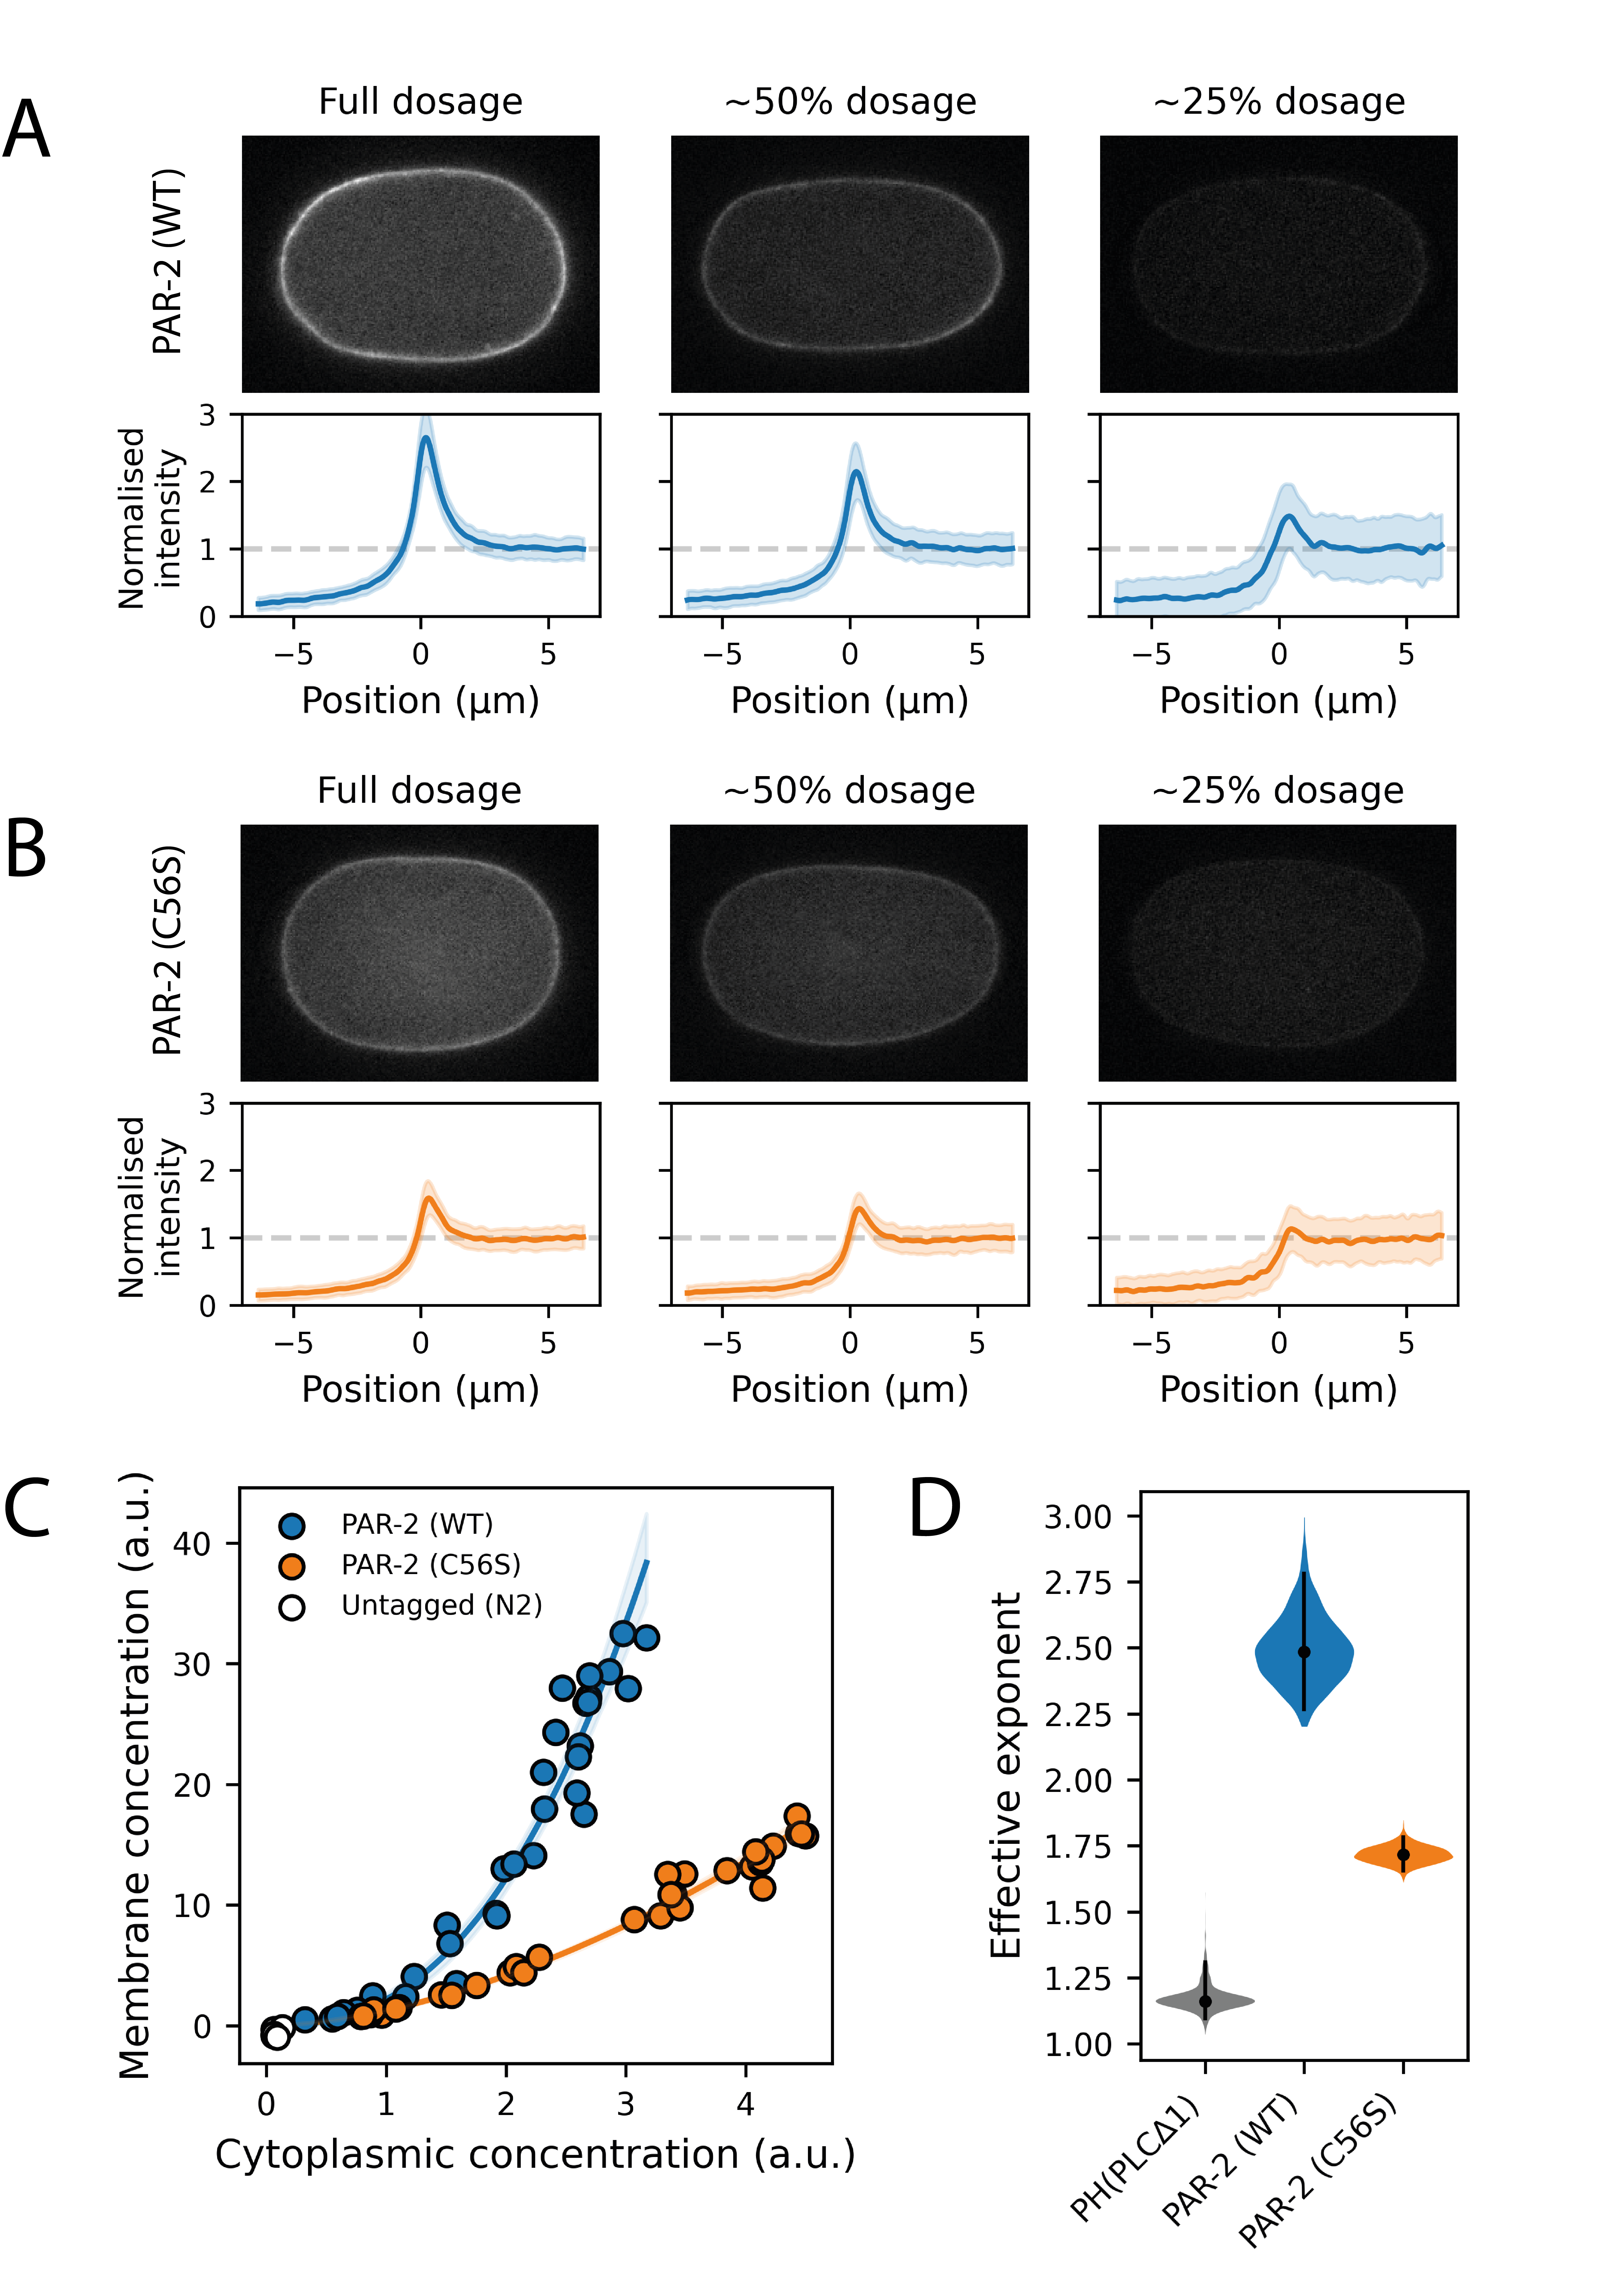
\includegraphics[scale=0.9]{rundown_vs_c56s_v2}
\centering
\mycaption{PAR-2 displays RING-dependent nonlinear membrane binding kinetics}{
\textbf{(A) - (B)} Images of \textit{par-3 (it71)} cells expressing wild type (A) or C56S (B) mNG::PAR-2 with varying dosage achieved by \textit{par-2 RNAi}. Bottom panels show mean ($\pm$ SD) normalised cross-cortex intensity profiles for the embryos shown, averaged over the entire embryo circumference.
\textbf{(C)} Quantification of membrane and cytoplasmic concentrations for the full dataset, including untagged N2s (white). Solid lines indicate fit of each dataset to an exponent model ($y = ax^b$). Shaded regions show 95\% confidence intervals, estimated by bootstrapping.
\textbf{(D)} Probability distributions of exponents from model fitting in (C), estimated by bootstrapping. PH(PLC$\Delta1$) data (derived from data in \cref{fig:memquant_benchmarking_ph_rundown}) shown for comparison. Vertical lines indicate 95\% confidence intervals.
}
\label{fig:rundown_vs_c56s}
\end{figure}

% I know that people will ask where polarised cells fit. For this particular dataset they seem to follow the same trajectory. However, I'm reluctant to include this as it seems to vary between datasets, as we've discussed previously. 

\section{Discussion}

Overall, these results show quantitative evidence for a PAR-2 driven positive feedback reaction, and a role for the RING domain in mediating this. I cannot exclude the possibility that nonlinearity might also depend on cooperative effects with other pPARs (LGL-1, PAR-1 and CHIN-1), as these were left intact in the assay. Further work would be required to determine this, although it is not clear how this would work, or why this would depend on the RING domain.\\

Previously, positive feedback has been suggested to underlie PAR-2's ability to polarise with uniform aPAR. However, my results reveal that, whilst some form of positive feedback appears to be present, this reaction displays no signs of intrinsic bistability, and therefore is insufficient to support polarity without additional asymmetries. This suggests that the network must have other features to generate spatial information in these contexts. One possibility is that LGL-1 and/or CHIN-1 might play an important role in inhibiting local aPAR activity. The distribution of these proteins in uniform aPAR conditions is not known, nor is PAR-2's dependence on these proteins for domain stability. Alternatively, PAR-2 itself might act to locally inhibit PKC-3 activity, perhaps via a tight association between PKC-3 and the FxR motif of PAR-2. However, the result that PAR-2(AxA) is less well removed by PKC-3 seems on the surface opposite to the idea that FxR may inhibit PKC-3. An alternative model might be that the microtubule cue persists and stabilises PAR-2 protection against PKC-3. However, this would not explain the inability of PAR-2(AxA) and PAR-2(C56S), which have no known microtubule-binding defects, to polarise in these conditions.\\

Nevertheless, the RING phenotype is striking, and suggests that the ability to reach high cortical concentrations, perhaps through a RING-mediated positive feedback reaction, is a requirement for stabilising pPAR domains. However, the precise mechanisms of PAR-2 RING domain action, and how this might lead to positive feedback, are unknown. This is the subject of investigation in the next chapter.\\


%%%%%%%%%%%%%%%%%%%%%%%%%%%%%%%%%%%%%%%%%%%%%%%%%%%%%%%%%%
\clearpage
\chapter{Determining mechanisms of PAR-2 RING domain action}

\textbf{Detailed contributions:}\\

Work in section \ref{section:ring_ubiquitin} was performed with Colin Davis in Anne Schreiber's lab, and Diego Esposito in Katrin Rittinger's lab, both at the Crick. Work in section \ref{section:ring_dimer} was performed with Dave Briggs in Neil McDonald's lab at the Crick.\\

\clearpage
\section{Introduction}

Whilst no mechanisms have been definitively attributed to the PAR-2 RING domain, several observations in previous studies provide insight into potential mechanisms. On its own, the PAR-2 RING domain has been shown to lack any membrane binding activity (\textcite{Hao2006}, and replicated later in \cref{fig:ring_fragment_in_vivo}), whereas a central portion of the protein containing the polybasic regions but lacking the RING domain binds to the membrane with a similar affinity to PAR-2 (C56S). Therefore, rather than a direct interaction with the membrane, it is likely that the RING domain plays a modulatory role. Additionally, the authors show that the weakened affinity of PAR-2 (C56S) cannot be restored by the presence of wild-type PAR-2.  I have also performed similar analysis in \cref{fig:c56s_cis}, which shows that PAR-2 (C56S) membrane affinity shows only a modest increase when balanced by a wild type copy compared to when homozygous. In other words, the effects of C56S mutation appear to be mostly cis-acting (intrinsic to each molecule). Finally, fluorescence recovery after photobleaching (FRAP) studies of PAR-2 (C56S) show that the mutant has faster membrane turnover kinetics than wild type PAR-2, suggesting that weakened membrane affinity in the mutant is due to a failure to stably associate with the membrane \citep{Motegi2011}.\\


\begin{figure}
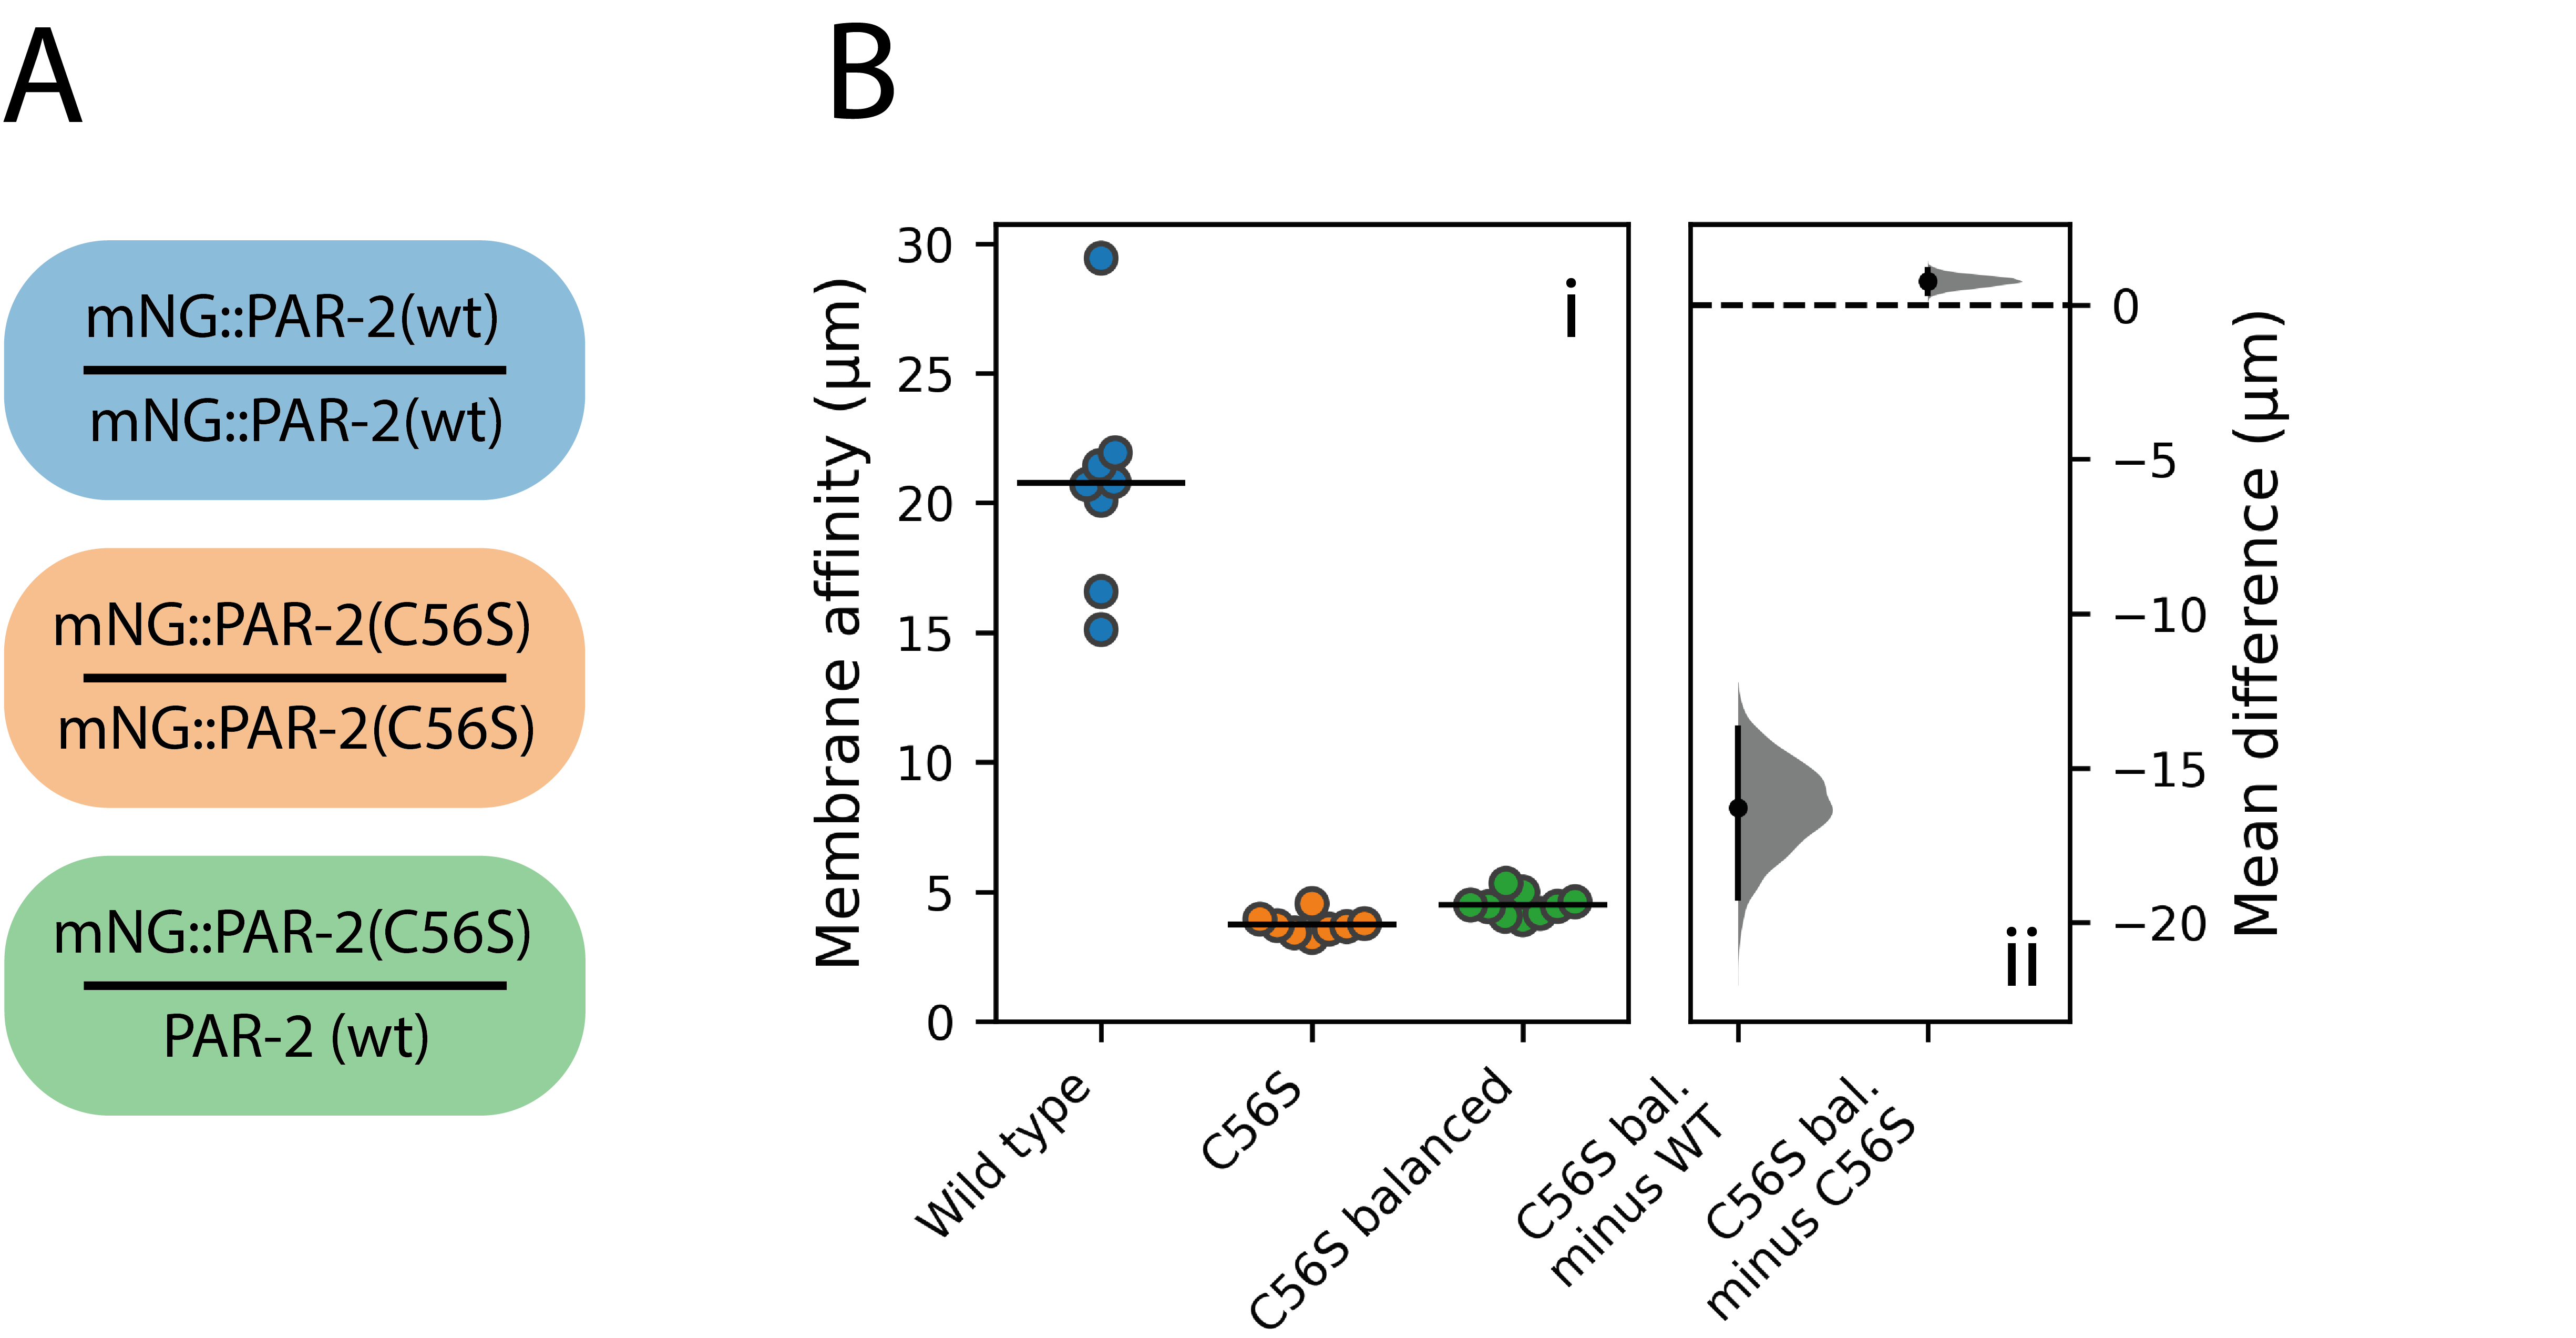
\includegraphics[scale=1.4]{c56s_cis_v2}
\centering
\mycaption{The PAR-2 RING domain activity is cis-acting}{
\textbf{(A)} Schematic of the three genotypes investigated. Quantification results represent the distribution of mNG-tagged PAR-2 only.
\textbf{(B)} i. Membrane affinity measurements for the three conditions, measured over the posterior domain of polarised cells.
ii. Probability distributions of effect sizes in the data, estimated by bootstrapping. Vertical bars indicate 95\% confidence intervals.
}
\label{fig:c56s_cis}
\end{figure}

RING domains were originally described by \textcite{Freemont1991} as a commonly occurring motif, between 40 and 70 residues in length, with a characteristic pattern of cysteine and/or histidine residues. Structural studies have since revealed a `cross-brace' pattern, whereby these cysteine and histidine residues interact with two zinc ions to form a characteristic folded structure (\cref{fig:ring_schematic}). RING domains are highly prevalent, with 300 RING domain containing genes in the human genome \citep{Li2008}. Two roles have been commonly attributed to RING domains in other proteins: ubiquitination and dimerisation. In this chapter, I investigate each of these in turn as potential mechanism in the context of PAR-2 membrane association.\\

\begin{SCfigure}
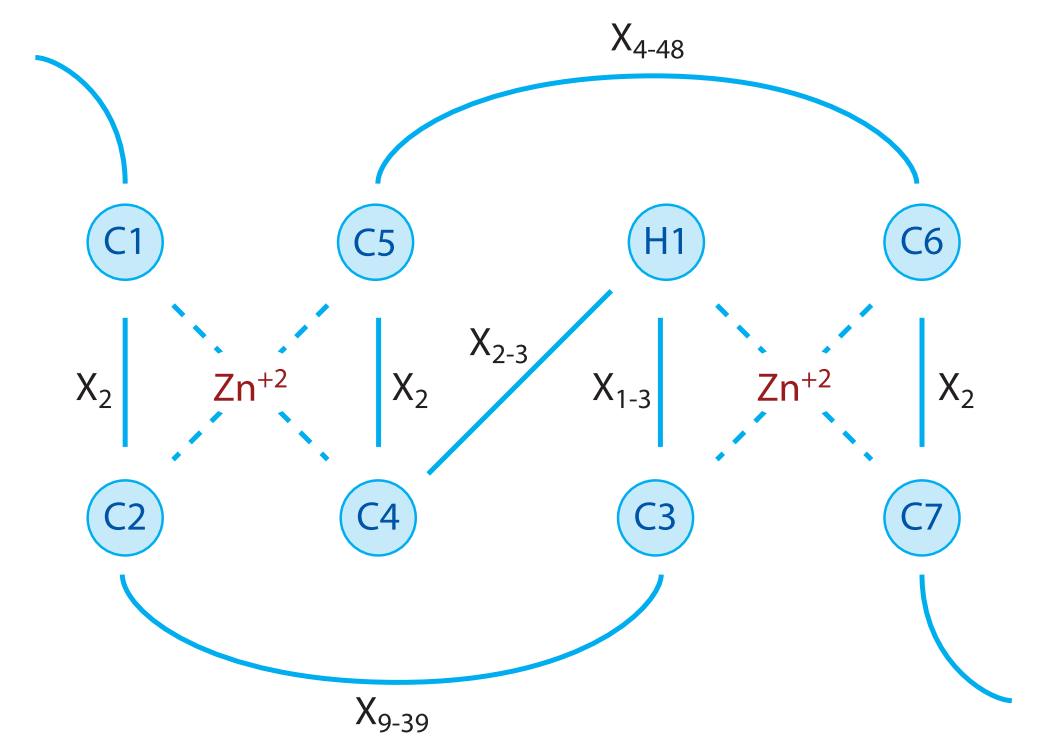
\includegraphics[scale=0.4]{ring_schematic}
\mycaption{Schematic of RING domain organisation}{
Cysteines interacting with zinc are labelled as C1 etc. H1 represents a zinc-interacting histidine. Xn refers to the number of amino acids in the spacer regions between the zinc ligands. Figure from \textcite{Deshaies2009}.
}
\label{fig:ring_schematic}
\end{SCfigure}


\section{Exploring a role for ubiquitination}
\label{section:ring_ubiquitin}

The most commonly associated role of RING domains is in the ubiquitination pathway, the mechanism by which ubiquitin (Ub) molecules are attached to substrate proteins. This pathway involves three classes of enzymes which catalyse three steps (\cref{fig:ubiquitination_pathway}): ubiquitin-activation (E1), ubiquitin-conjugation (E2), ubiquitin-ligation (E3), the latter of which is commonly attributed to RING domain proteins. E1 activates ubiquitin and transfers to an E2, where a thioester bond is formed between the E2 and Ub. E3s then simultaneously interact with a substrate and the E2-Ub conjugate to catalyse the transfer of Ub to a target lysine on the substrate. \\

\begin{figure}[!h]
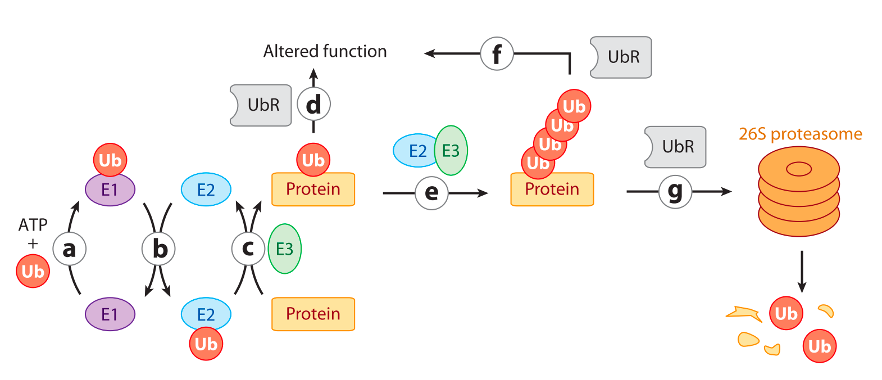
\includegraphics[scale=0.95]{ubiquitination_pathway}
\setlength{\abovecaptionskip}{20pt}
\centering
\mycaption{Schematic of the ubiquitination pathway}{Figure from \cite{Deshaies2009}}
\label{fig:ubiquitination_pathway}
\end{figure}

A single E1 can work with several E2s ($\sim$ 40 in humans, 22 in \textit{C. elegans}), which work with hundreds of E3s. The choice of E2 often determines the type of ubiquitination that occurs. This can be either monoubiquitination, where a single ubiquitin molecule is added to a target lysine, or polyubiquitination, meaning the formation of a ubiquitin chain via lysine molecules on ubiquitin monomers. The functional consequences of ubiquitination are directly related to the type of ubiquitination that occurs. Monoubiquitination is associated with modification of protein function, and can regulate the structure of a protein, change its binding partners or change its cellular localisation. Depending on the type of linkage, polyubiquitination can also be associated with modification of protein function, but is most commonly associated with proteasome-dependent proteolysis. Each E3 typically interacts with only a small number of E2s, and a small number of substrates. Therefore, by acting as a bridge between a specific E2 and a specific substrate, E3s are responsible for conferring specificity to the ubiquitination reaction. \\

It is thought that most RING domain proteins possess E3 ligase activity \citep{Deshaies2009}, catalysing the transfer of Ub directly from an E2 to a target substrate. RING E3s work by binding to and stabilising the `closed' conformation of an E2-Ub conjugate. This alters the geometry of the thioester bond between Ub and E2, increasing reactivity towards a substrate lysine residue. At the same time as interacting with the E2, most RING E3s bind to a substrate, bringing a specific lysine on the substrate into close proximity of the E2. This then leads to direct transfer of Ub from the E2 to the substrate. Typically, this E3/substrate interaction is via other parts of the E3 protein, rather than the RING domain itself (e.g. the TRIM class of E3s use C-terminal substrate recognition domains).\\

Alternatively, lysines on the E3 protein itself can be targeted (autoubiquitination). In many cases this may be a side effect of E3 activity with no functional role, but in some cases this may serve a purpose. For example, autoubiquitination of BCA2 has been demonstrated as an elegant mechanism to regulate steady state levels of the protein \citep{Amemiya2008}. As autoubiquitination drives degradation, and is competitive with substrate ubiquitination, the protein is able to regulate its own levels according to substrate availability.\\

Given the common role for RING domain proteins as ubiquitin ligases, this function has long been suspected for PAR-2, possibly as a mechanism to locally exclude or degrade PKC-3. Parallels have been drawn to the \textit{Drosophila} E3 ubiquitin ligase Slimb, which is required for the accumulation of Par-1 in oocytes, and is thought to work by locally degrading aPKC \citep{Eurico-de-Sa2014, Skwarek2014}. Definitive evidence for ubiquitin ligase activity by PAR-2 has so far not been demonstrated, but yeast two hybrid assays show that PAR-2 interacts modestly with several E2 enzymes \citep{Gudgen2004}.\\

Whilst ubiquitination of other targets may be important, similar to Slimb, the fact that the localisation defects of the PAR-2 (C56S) mutant cannot be rescued in trans suggests that, if ubiquitination activity contributes to membrane localisation, this must be a cis-acting function. Given that autoubiquitination is common for E3s, and that ubiquitination can change the properties of a protein, it is plausible that the defects observed in C56S mutants may relate to a failure to autoubiquitinate. In this section I aim to test PAR-2 for ubiquitination activity, and investigate the potential role of this in vivo.\\

\subsection{PAR-2 does not show activity in in vitro ubiquitination assays}

My first aim was to test for the ability of PAR-2 to act as a ubiquitin ligase. Typically, this property can be assayed in vitro using purified samples of a protein of interest. To express and purify PAR-2 we used an insect cell system, which was chosen for its ability to express high levels of large, complex proteins. We expressed strep-tagged full-length PAR-2 in insect cells, lysed cells by sonication, and purified by strep pull-down followed by size exclusion chromatography (SEC) (see Methods). From the initial pull-down stage, we observed two prominant bands close to the expected mass of PAR-2. Due to their similar masess, we were unable to separate the two bands by size exclusion chromatography (\cref{fig:ubiquitin_assay}A). We tested both bands by mass spectrometry, which confirmed them both to be PAR-2. Interestingly, a single site (K351) was found to be ubiquitinated in the sample corresponding to the upper band, explaining the higher mass of this population on the gel compared to the expected mass of strep-tagged PAR-2 (75.24 kDa). No ubiquitinated sites were found in the sample corresponding to the lower band, which sits closer to the expected weight of PAR-2, although the K351 site was not covered by mass spectrometry results, so we cannot confirm that this site was not ubiquitinated. We also observed two similar bands in a small-scale prep of PAR-2 (C56S) (data not shown). Therefore, I do not believe this to be a result of autoubiquitination, but may rather represent ubiquitination of the protein by an insect ubiquitin ligase within the insect cells. CRISPR mutation of K351 to an alanine has no effect on PAR-2 localisation in vivo (data not shown), and previous attempts to purify PAR-2 from worm lysates and HEK cell preps have not shown a high molecular weight population.\\

The sample from SEC purification was pooled (lanes 1-9) and used for an in vitro ubiquitination assay. Designed to test for ubiquitination activity of a protein, this assay involves mixing a test protein with ubiquitin, E1 and an E2, and looking for autoubiquitination of the test protein (see Methods). Given that E3s typically work with only a small number of E2s, the assay is sensitive to the choice of E2, and therefore care must be taken to choose an appropriate E2. In the case of PAR-2 this is so far unknown, although PAR-2 has been shown to weakly interact with UBC-2, UBC-18 and UEV-2 in yeast two hybrid assays \citep{Gudgen2004}. Since UBC-2 (known as UBCH5a in Humans) is also the most promiscuous of the E2s, this was chosen for the assay. As shown in \cref{fig:ubiquitin_assay}, whereas a positive control sample (TRIM2) showed rapid auto-polyubiquitination and depletion of the ubiquitin pool within 30 minutes, no effect was observed for PAR-2 across the whole 60 minutes of the assay, indicating lack of detectable ubiquitination activity. A similar assay was performed using human UBC13/UEV1 as the E2, chosen based on PAR-2's sequence similarity to the E3 ligase RNF8, which works with this E2, however the result of this was also negative (data not shown).\\

\begin{figure}
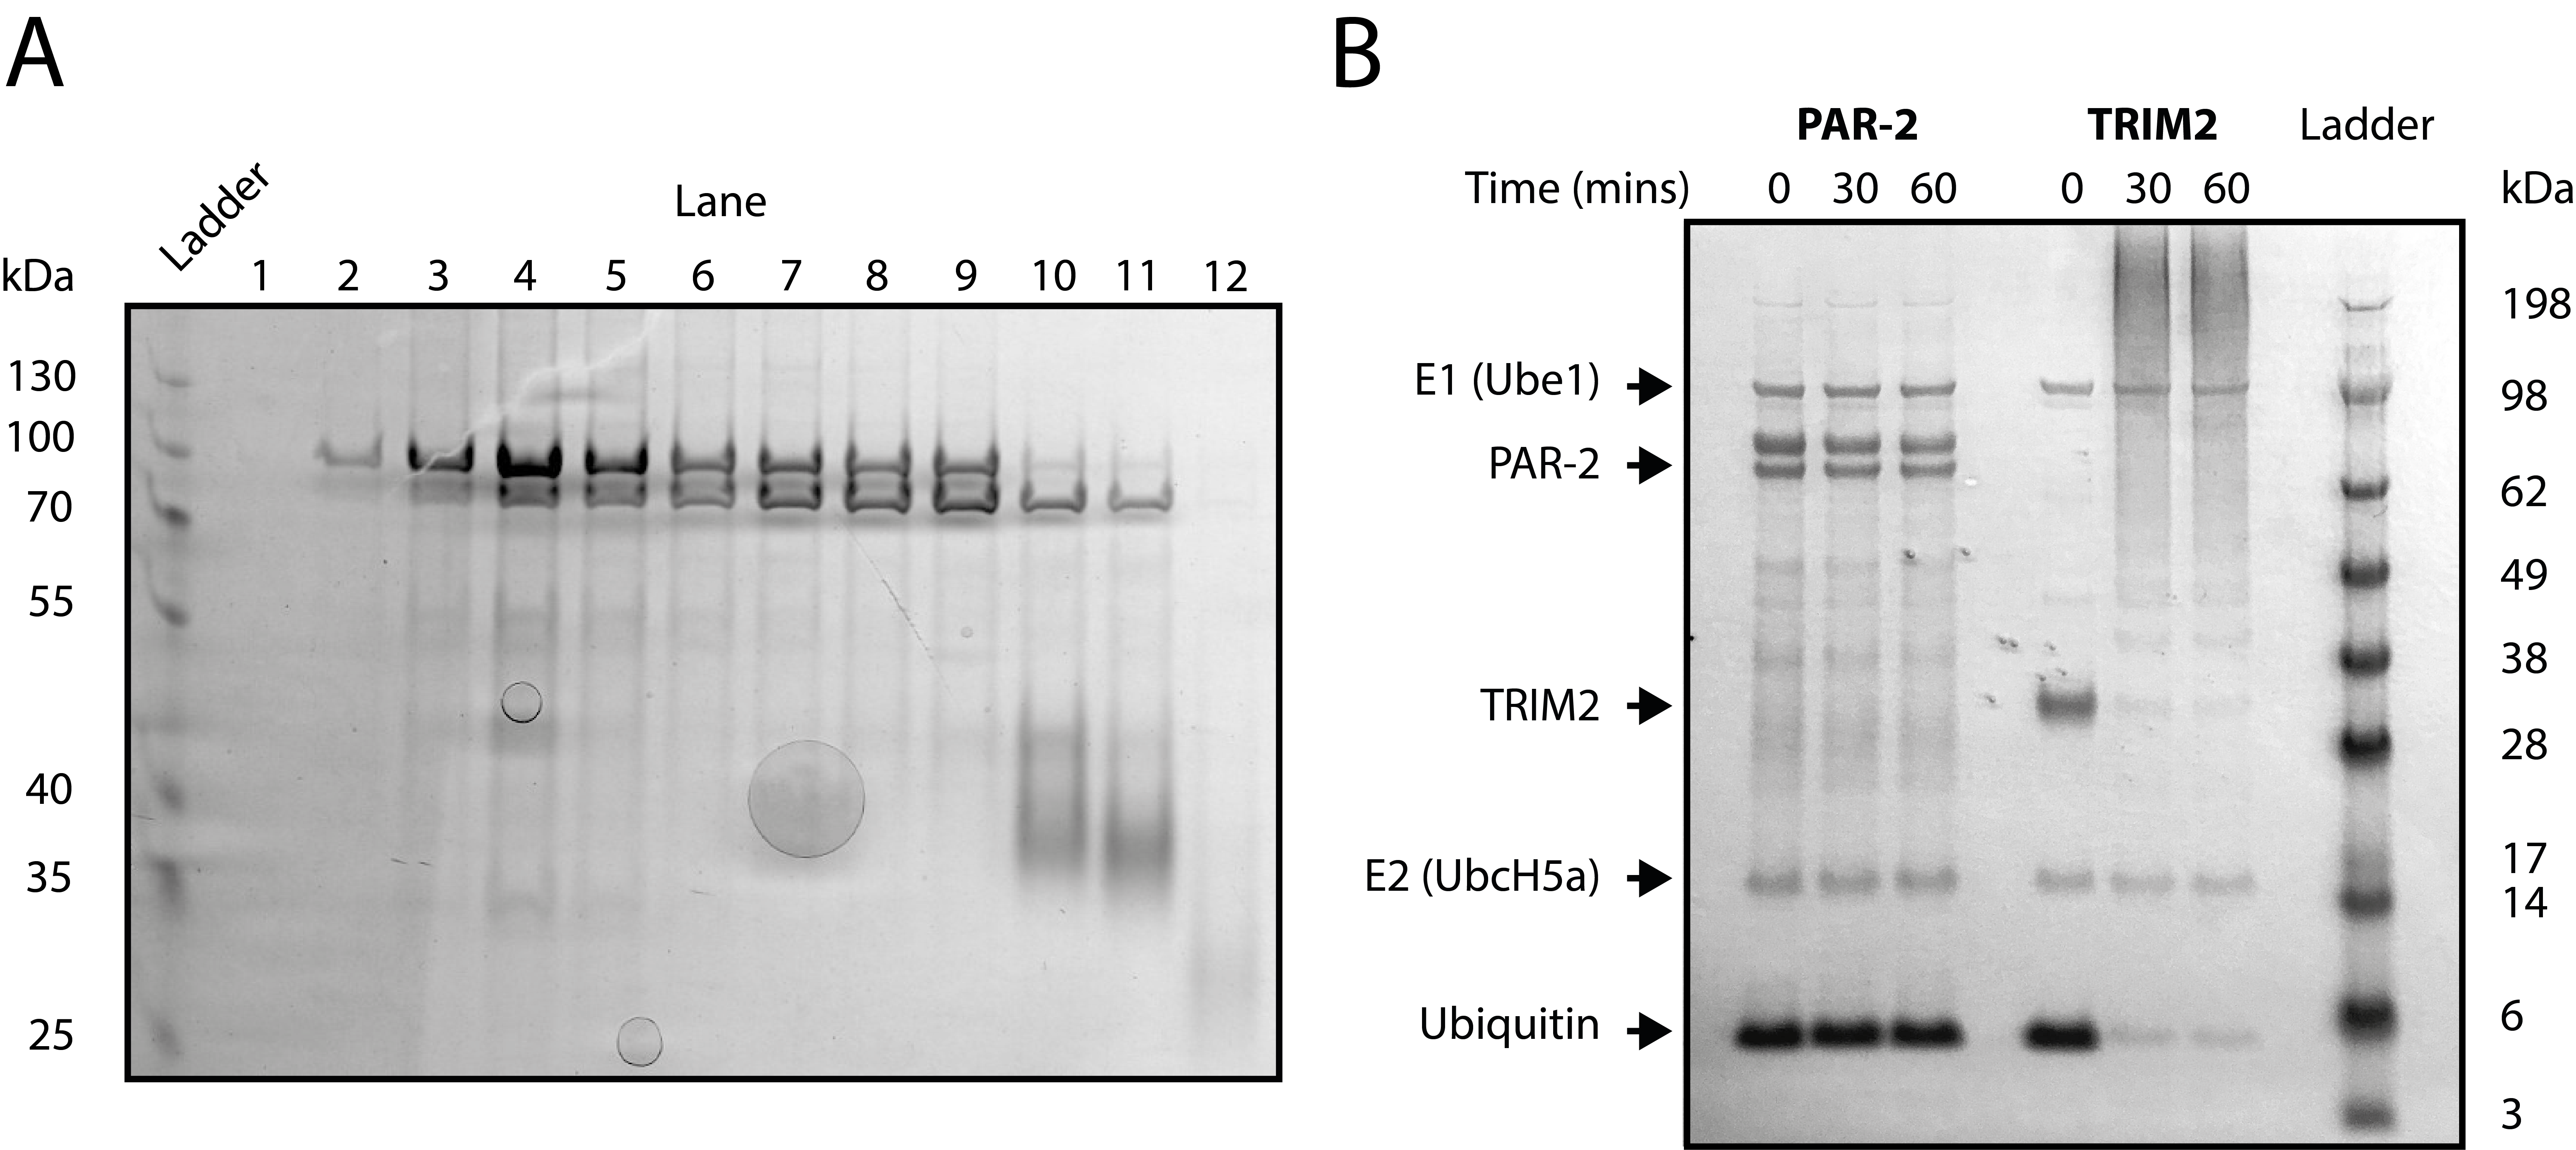
\includegraphics[scale=1]{ubiquitin_assay}
\centering
\mycaption{PAR-2 does not show activity in an in vitro ubiquitination assay}{
\textbf{(A)} Size exclusion chromatography results for a sample of strep-tagged PAR-2 purified from insect cells. The two prominent bands in the 70-100 kDa region both contain PAR-2. Expected weight (with strep tag) = 75.24 kDa.
\textbf{(B)} Ubiquitination assay results for PAR-2 vs TRIM2. Whereas TRIM2 displays auto-polyubiquitination activity, as shown by the appearance of 'streak' at high masses representing polyubiquitinated protein, loss of unmodified TRIM2 and loss of free ubiquitin, no activity is observed for PAR-2 throughout the entire assay. 
}
\label{fig:ubiquitin_assay}
\end{figure}


\subsection{Targeted mutation to putative linchpin site has no phenotype}

Whilst C56S mutation has a clear and strong effect in vivo, this does not necessarily imply a role for PAR-2 as a ubiquitin ligase, as unfolding the domain by mutating a zinc-coordinating residue may have a multitude of disruptive effects. Therefore, to test the potential role of ubiquitination in vivo, I aimed to specifically disrupt E3 ligase activity without disrupting the core structure of the RING domain.\\

Whilst mechanisms of catalytic activity are variable among proteins, a key catalytic site found in many RING E3 ligases is an arginine or lysine residue immediately downstream of the final zinc-coordinating cysteine, known as the `linchpin site', which forms a hydrogen bond with the E2 to stabilise the closed (active) state of the E2 \citep{Pruneda2012}. Mutation of this site to an alanine has been shown, for several proteins, to abrogate RING domain catalytic activity \citep{Pruneda2012}. Typically, the choice of residue at this site regulates a trade-off between ubiquitination activity and E2 specificity. RINGs with a K at this site typically show lower ubiquitination activity in vitro but higher E2 specificity. \textcite{Stewart2017} showed for the protein BRCA1 that mutating this site from an arginine to a lysine increases ubiquitination activity but reduces E2 specificity. 46\% of human RING domains have an arginine at this site, whereas 14\% have lysine \citep{Stewart2017}. However, many known RING E3 ligases have neither an arginine or lysine at this site (such as several members of the TRIM family of RING E3 ligases, \cref{fig:linchpin_alignments}B), suggesting that other mechanisms of E2 activation must exist. Currently this is poorly understood.\\

\textit{C. elegans} PAR-2 has a lysine at the canonical linchpin site, which suggests that the standard linchpin mechanism for E2 activation could apply. Alignment of \textit{Caenorhabditis} PAR-2 RING domain sequences shows that this site is largely conserved as a lysine across the genus (\cref{fig:linchpin_alignments}A), but \textit{C. bovis}, \textit{C. castelli} and \textit{C. monodelphis} have neither an arginine nor a lysine at this site. The fact that this site is not universally conserved may argue against an important role for ubiquitination activity, could suggest that PAR-2 does play an role as a ubiquitin ligase but does not rely on the linchpin mechanism, or could suggest that these other species have evolved alternative strategies distinct from \textit{C. elegans}.\\ 

\begin{figure}
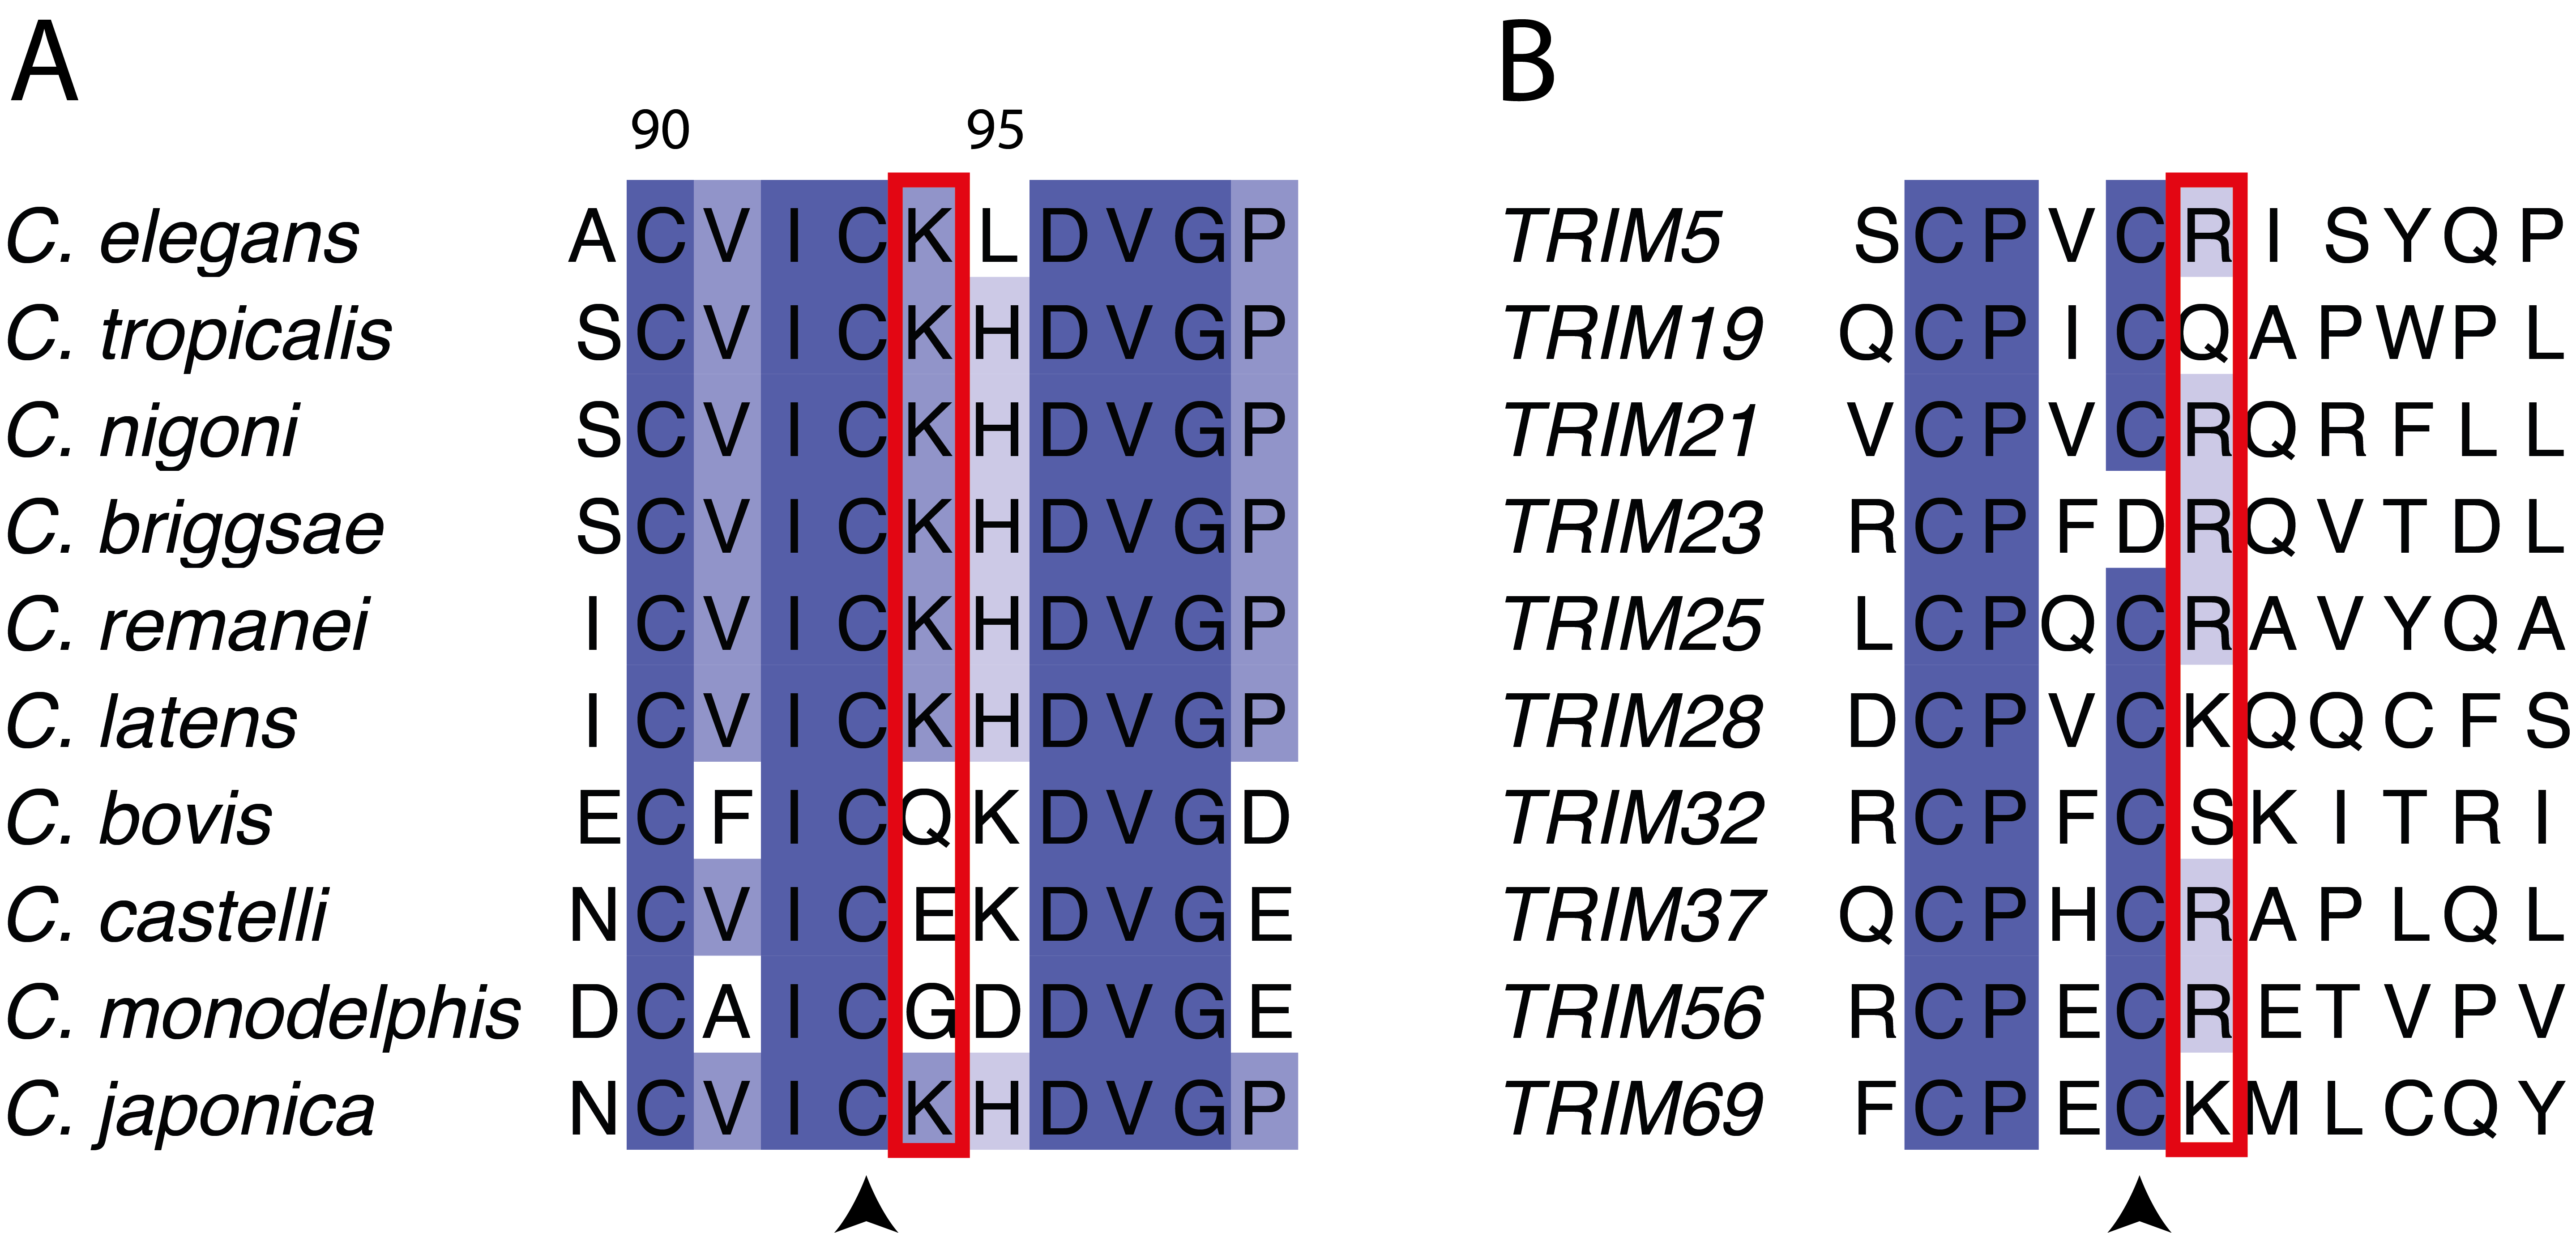
\includegraphics[scale=0.9]{linchpin_alignments}
\centering
\mycaption{Linchpin site alignments}{
\textbf{(A)} Alignment for the PAR-2 linchpin site (red box) across species of the \textit{Caenorhabditis} genus. This site is largely conserved as a lysine, but some species do not follow this pattern.
\textbf{(B)} Alignment of the linchpin site across the TRIM family of ubiquitin ligase proteins. In most cases this is an arginine or a lysine, but in some cases a different amino acid is present.
}
\label{fig:linchpin_alignments}
\end{figure}

To test the potential role of linchpin-mediated autoubiquitination for PAR-2 membrane binding affinity, I used CRISPR to perform targeted mutation to this site, turning it into an alanine. As shown in \cref{fig:linchpin_in_vivo}, this has only a marginal effect on membrane affinity. Whilst this cannot rule out a role for PAR-2 as a ubiquitin ligase in vivo, the result argues against a model in which linchpin-mediated autoubiquitination is a main driver of high membrane association.\\

\begin{figure}
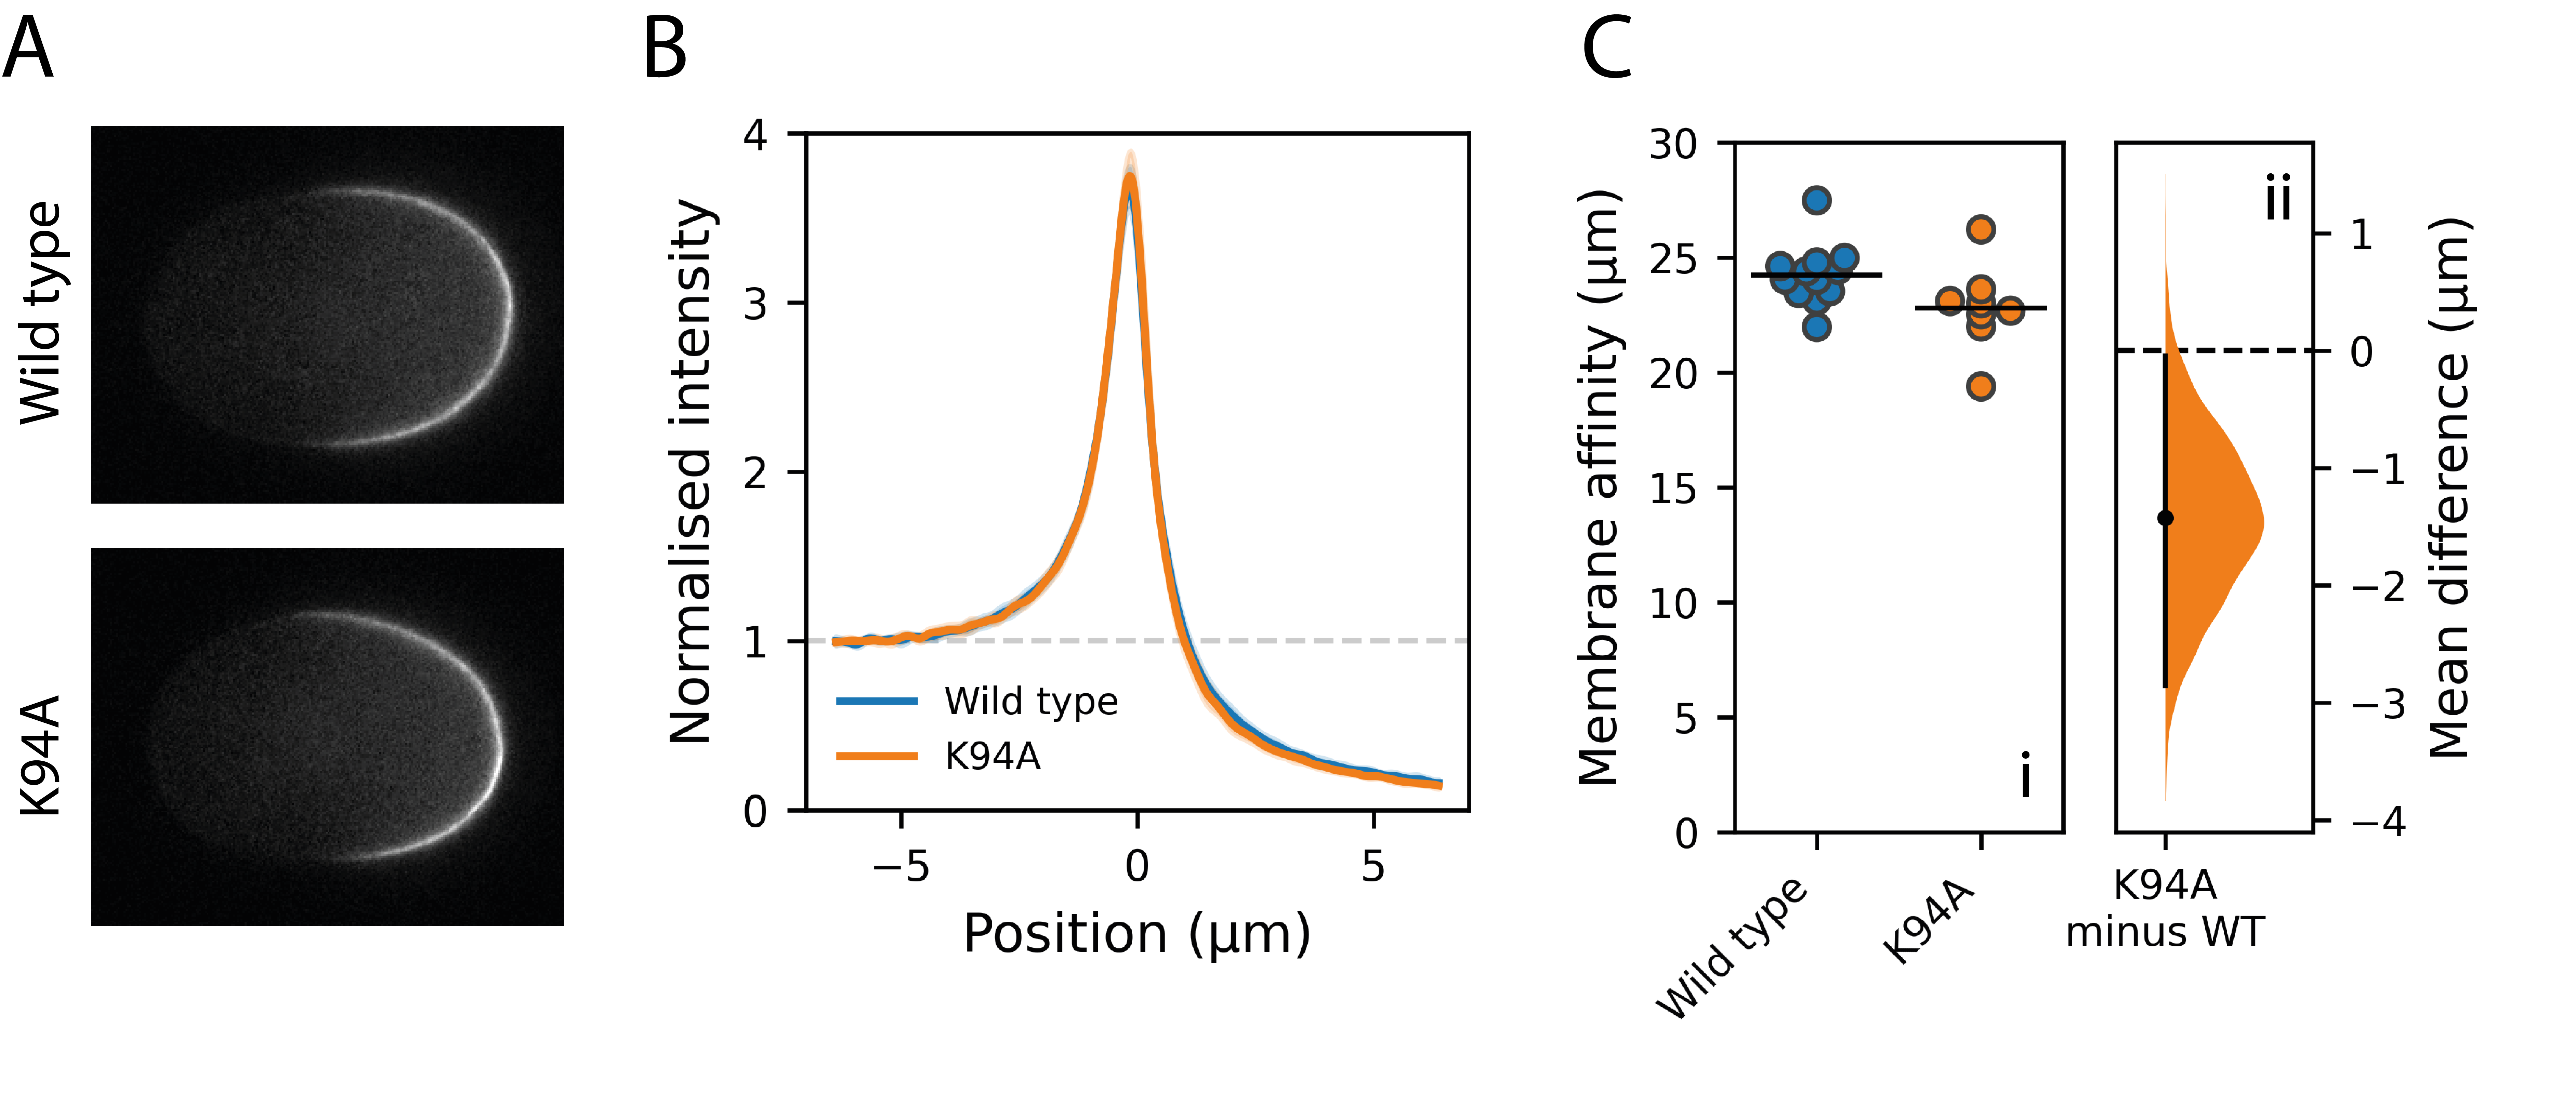
\includegraphics[scale=0.9]{linchpin_in_vivo_v2}
\centering
\mycaption{Mutation of the PAR-2 linchpin site has no effect on membrane affinity}{
\textbf{(A)} Midplane images of wild type vs K94A GFP::PAR-2 at maintenance phase.
\textbf{(B)} Normalised cross-cortex profiles for wild type vs K94A PAR-2 averaged over the posterior domain.
\textbf{(C)} i. Membrane affinity measurements for wild type vs K94A PAR-2 in the posterior domain.
ii. Probability distribution of the mean membrane affinity difference between wild type and K94A PAR-2, estimated by bootstrapping. Vertical line indicates 95\% confidence interval.
}
\label{fig:linchpin_in_vivo}
\end{figure}


\subsection{Discussion}

Whilst the results in this section do not provide evidence to support PAR-2 ubiquitin ligase activity, it is difficult to draw strong conclusions. Negative results in the ubiquitination assay could indicate lack of E3 ligase activity, but may have also been caused by an inappropriate E2, damage to the protein during purification, or there could be a low level of activity that is below the detection threshold of the assay. The first point could be addressed by using an E2 scan, an approach that tests for activity using a wide array of available E2s, but this has not yet been explored. Negative results for the linchpin mutant could argue that PAR-2 does not act as an E3 ligase (at least not in a way that would impact membrane affinity), but given that the linchpin mechanism is not universally conserved in E3s, ubiquitination activity cannot be ruled out.\\

% other possible ways of disrupting E2 interaction?

\clearpage
\section{Exploring a role for dimerisation}
\label{section:ring_dimer}

Another key function attributed to RING domains is their ability to act as dimerisation domains. Many purified RING domains have been shown to self-associate in crystal structures, forming dimers or higher order oligomers. In most cases, dimerisation is achieved via hydrophobic interactions between short alpha-helical segments N and C terminal of the core RING domain (N helix and C helix), which form a four-helix bundle, as well as additional hydrophobic contacts in the core RING domain (\cref{fig:trim25}). \\


\begin{SCfigure}
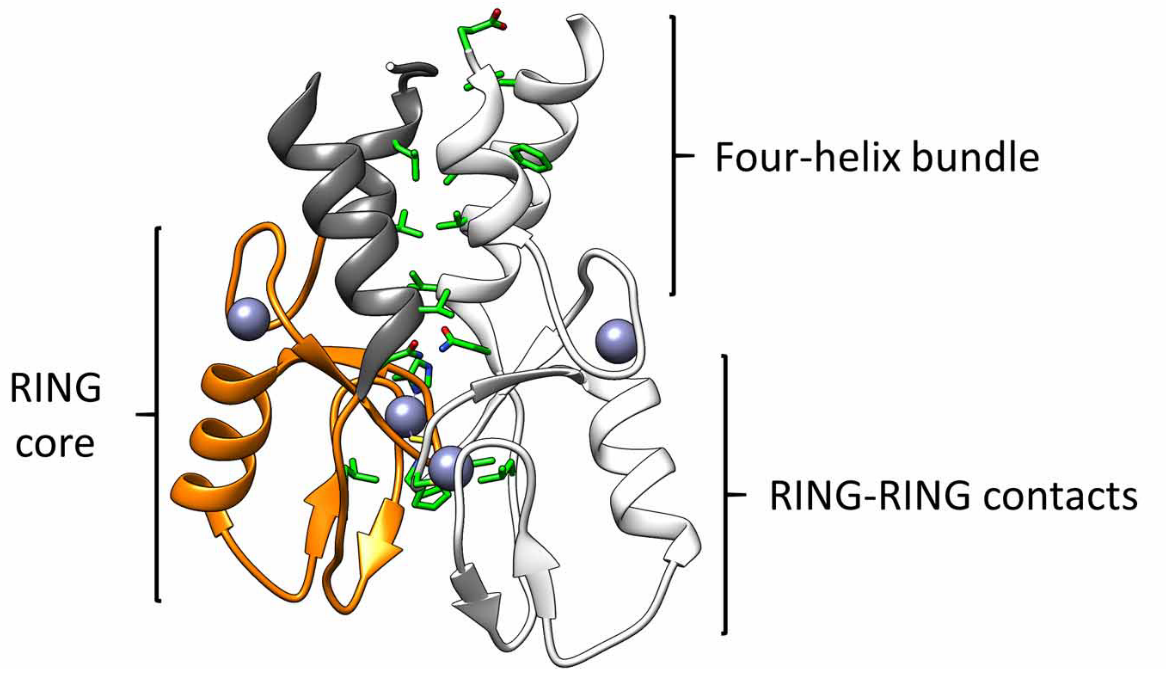
\includegraphics[scale=0.4]{trim25}
\mycaption{Structure of the TRIM25 RING domain dimer}{
A RING domain consisting of a zinc-interacting core (orange) flanked by N and C helices (dark gray) interacts with a second RING domain (white) to form a dimer. The dimer interface is characterised by a four-helix bundle and additional contacts between the RING cores. Hydrophobic residues at the interface are highlighted in green. Figure from \textcite{Fiorentini2020}.
}
\label{fig:trim25}
\end{SCfigure}

In many cases, the significance of dimerisation is fundamentally linked to the role of RING-domain proteins as ubiquitin ligases. RING dimerisation helps stabilise the closed E2-Ub conformation, by allowing each Ub to make simultaneous contacts with two RING domains, which in many cases is essential for ubiquitination activity. Mutations to key hydrophobic residues in N and C helices have been shown to disrupt dimerisation and reduce ubiquitination activity for many RING domains \citep{Koliopoulos2016, Rojas-Fernandez2014, Liew2010}. On the other hand, forced dimerisation of RINGs can hyperactivate ubiquitination activity, as has been shown for RNF4 \citep{Rojas-Fernandez2014}. Given the widespread roles of protein dimerisation \citep{Goodsell2000}, it is also not unlikely that RING domains have evolved functions as dimerisation domains in other contexts unrelated to ubiquitination, however to the best of my knowledge there are no confirmed examples of this to date.\\

Whilst the majority of RING domains are dimeric in crystal structures, their oligomeric state in solution varies dramatically, ranging from entirely monomeric to constitutively dimeric. For example, whereas TRIM32 appears constitutively dimeric in solution \citep{Koliopoulos2016}, TRIM21 exists in a monomer-dimer equilibrium \citep{Dickson2018}, and TRIM25, whilst crystalising as a dimer, appears entirely monomeric in solution, only dimerising at very high concentrations \citep{Koliopoulos2016}. \\

% comment on this, related to interface size?, deltaG? 

In the case of RING domains at the weaker end of the dimerisation scale, which exist largely as monomers in isolation, the ability to dimerise may be context specific. RNF4 is largely monomeric at physiological concentrations in vitro, but is able to dimerise upon addition of its substrate. Dual binding of two RNF4 molecules to a single substrate molecule creates a locally high concentration of RNF4 that permits dimerisation, which may be a mechanism for ensuring substrate-specific activation \citep{Rojas-Fernandez2014}. Similarly, TRIM25 shows weak dimerisation ability on its own, but dimerisation is stabilised by binding to an E2. \\

Notably, however, not all RING domains are dimeric. Some form higher order structures (e.g. the TRIM19 RING, which forms a `torus-shaped' tetramer in crystal structures \citep{Wang2018}), whereas others lack any ability to oligomerise. The TRIM28 RING domain, for example, has a small N helix, but lacks a C helix, and forms no dimerisation contacts in crystal structures \citep{Stevens2019}. The TRIM56 RING domain lacks both helices, and similarly is monomeric in crystal structures \citep{Fiskin2017}.\\

% Likewise, the CBL class of RING domains <more>..

In the case of PAR-2, the potential role for the RING domain as a dimerisation domain has not been tested, however full-length PAR-2 has been suggested to oligomerise. In vitro pull downs (\cite{Motegi2011}, \cite{Arata2016}) show that PAR-2 can weakly self-associate. \textcite{Arata2016} further showed by TIRF imaging that cortical PAR-2 exists as particles of varying size, which may represent a mix of monomers, dimers and possibly larger oligomers (they estimate that the largest oligomers are tetrameric). In this section, I aim to test the dimerisation properties of the PAR-2 RING domain, and investigate the potential importance of this in vivo.\\

\subsection{PAR-2 RING domain sequence bears hallmarks of dimeric RINGs}

To investigate the potential role of the PAR-2 RING as a dimerisation domain, I began by analysing the sequence of the domain. I performed a BLAST search to compare the PAR-2 sequence against sequences of proteins for which the quaternary structure has been solved using laboratory methods, using the online SWISS model tool. This showed that the PAR-2 RING has sequence similarity to a number of well-characterised RING domains, most of which are dimeric in their crystal structures (\cref{tab:rings_pdb}). Sequence alignment shows that the PAR-2 sequence displays the general pattern of hydrophobic residues expected at the N and C helices of dimeric RING domains (\cref{fig:alignments_other_rings}).\\

\begin{table}[]
\centering
\begin{tabular}{|l|l|l|}
\hline
\textbf{Protein} & \textbf{PDB code} & \textbf{Quaternary structure} \\ \hline
TRIM69 & 6YXE & Dimer \\ \hline
RAD18 & 2Y43 & Dimer \\ \hline
RNF8 & 4AYC & Tetramer \\ \hline
TRIM21 & 6FGA & Dimer \\ \hline
TRIM25 & 5EYA & Dimer \\ \hline
TRIM5 & 4TKP & Monomer \\ \hline
\end{tabular}
\mycaption{RING domain proteins in the Protein Data Bank (PDB) with closest homology to the PAR-2 RING domain}{}
\label{tab:rings_pdb}
\end{table}

\begin{figure}
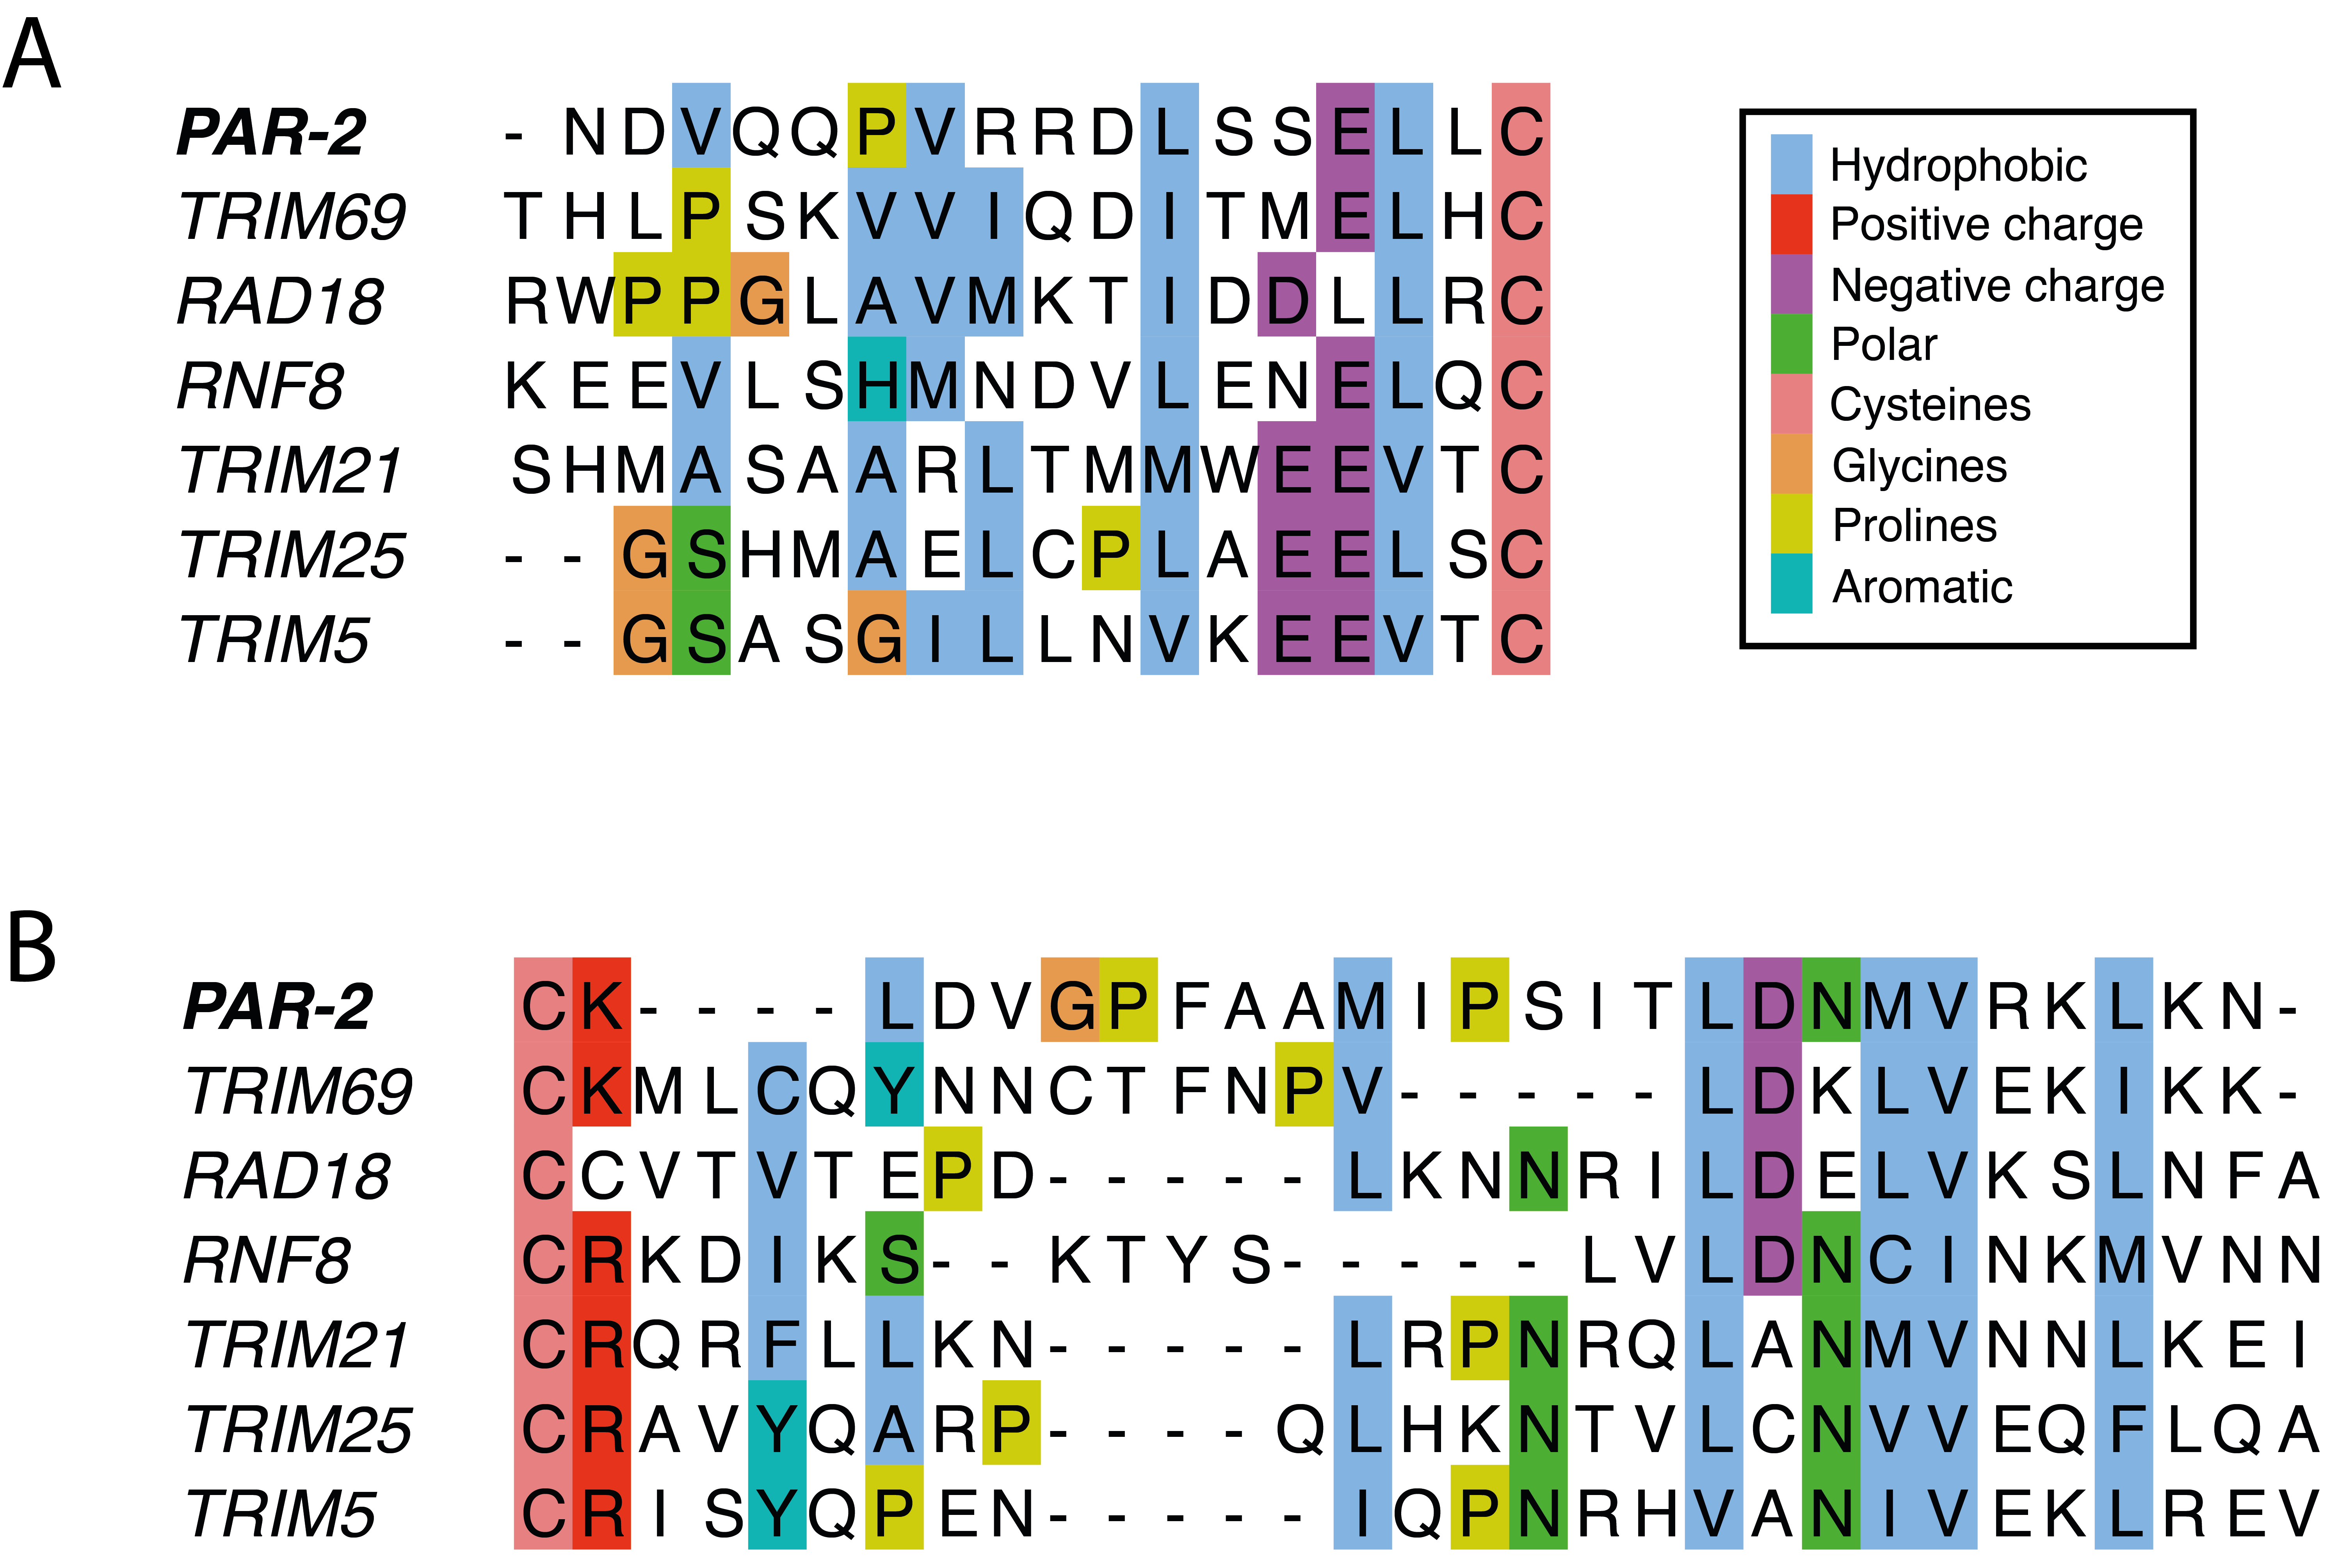
\includegraphics[scale=1]{alignments_other_rings}
\centering
\mycaption{Alignment of the PAR-2 RING domain N and C helices against similar proteins in the PDB}{
\textbf{(A)} N-helix alignment. Arrowhead indicates first zinc-coordinating cysteine of the core RING domain.
\textbf{(B)} C-helix alignment. Arrowhead indicates final zinc-coordinating cysteine of the core RING domain. Hydrophobic residues indicated in blue.
}
\label{fig:alignments_other_rings}
\end{figure}

These regions are also highly conserved in different \textit{Caenorhabditis} species (\cref{fig:alignments_par2}). Whilst there is some sequence variation, almost all species have an identical pattern of hydrophobic residues, which points to a potentially important role for PAR-2 RING domain dimerisation. \\

\begin{figure}
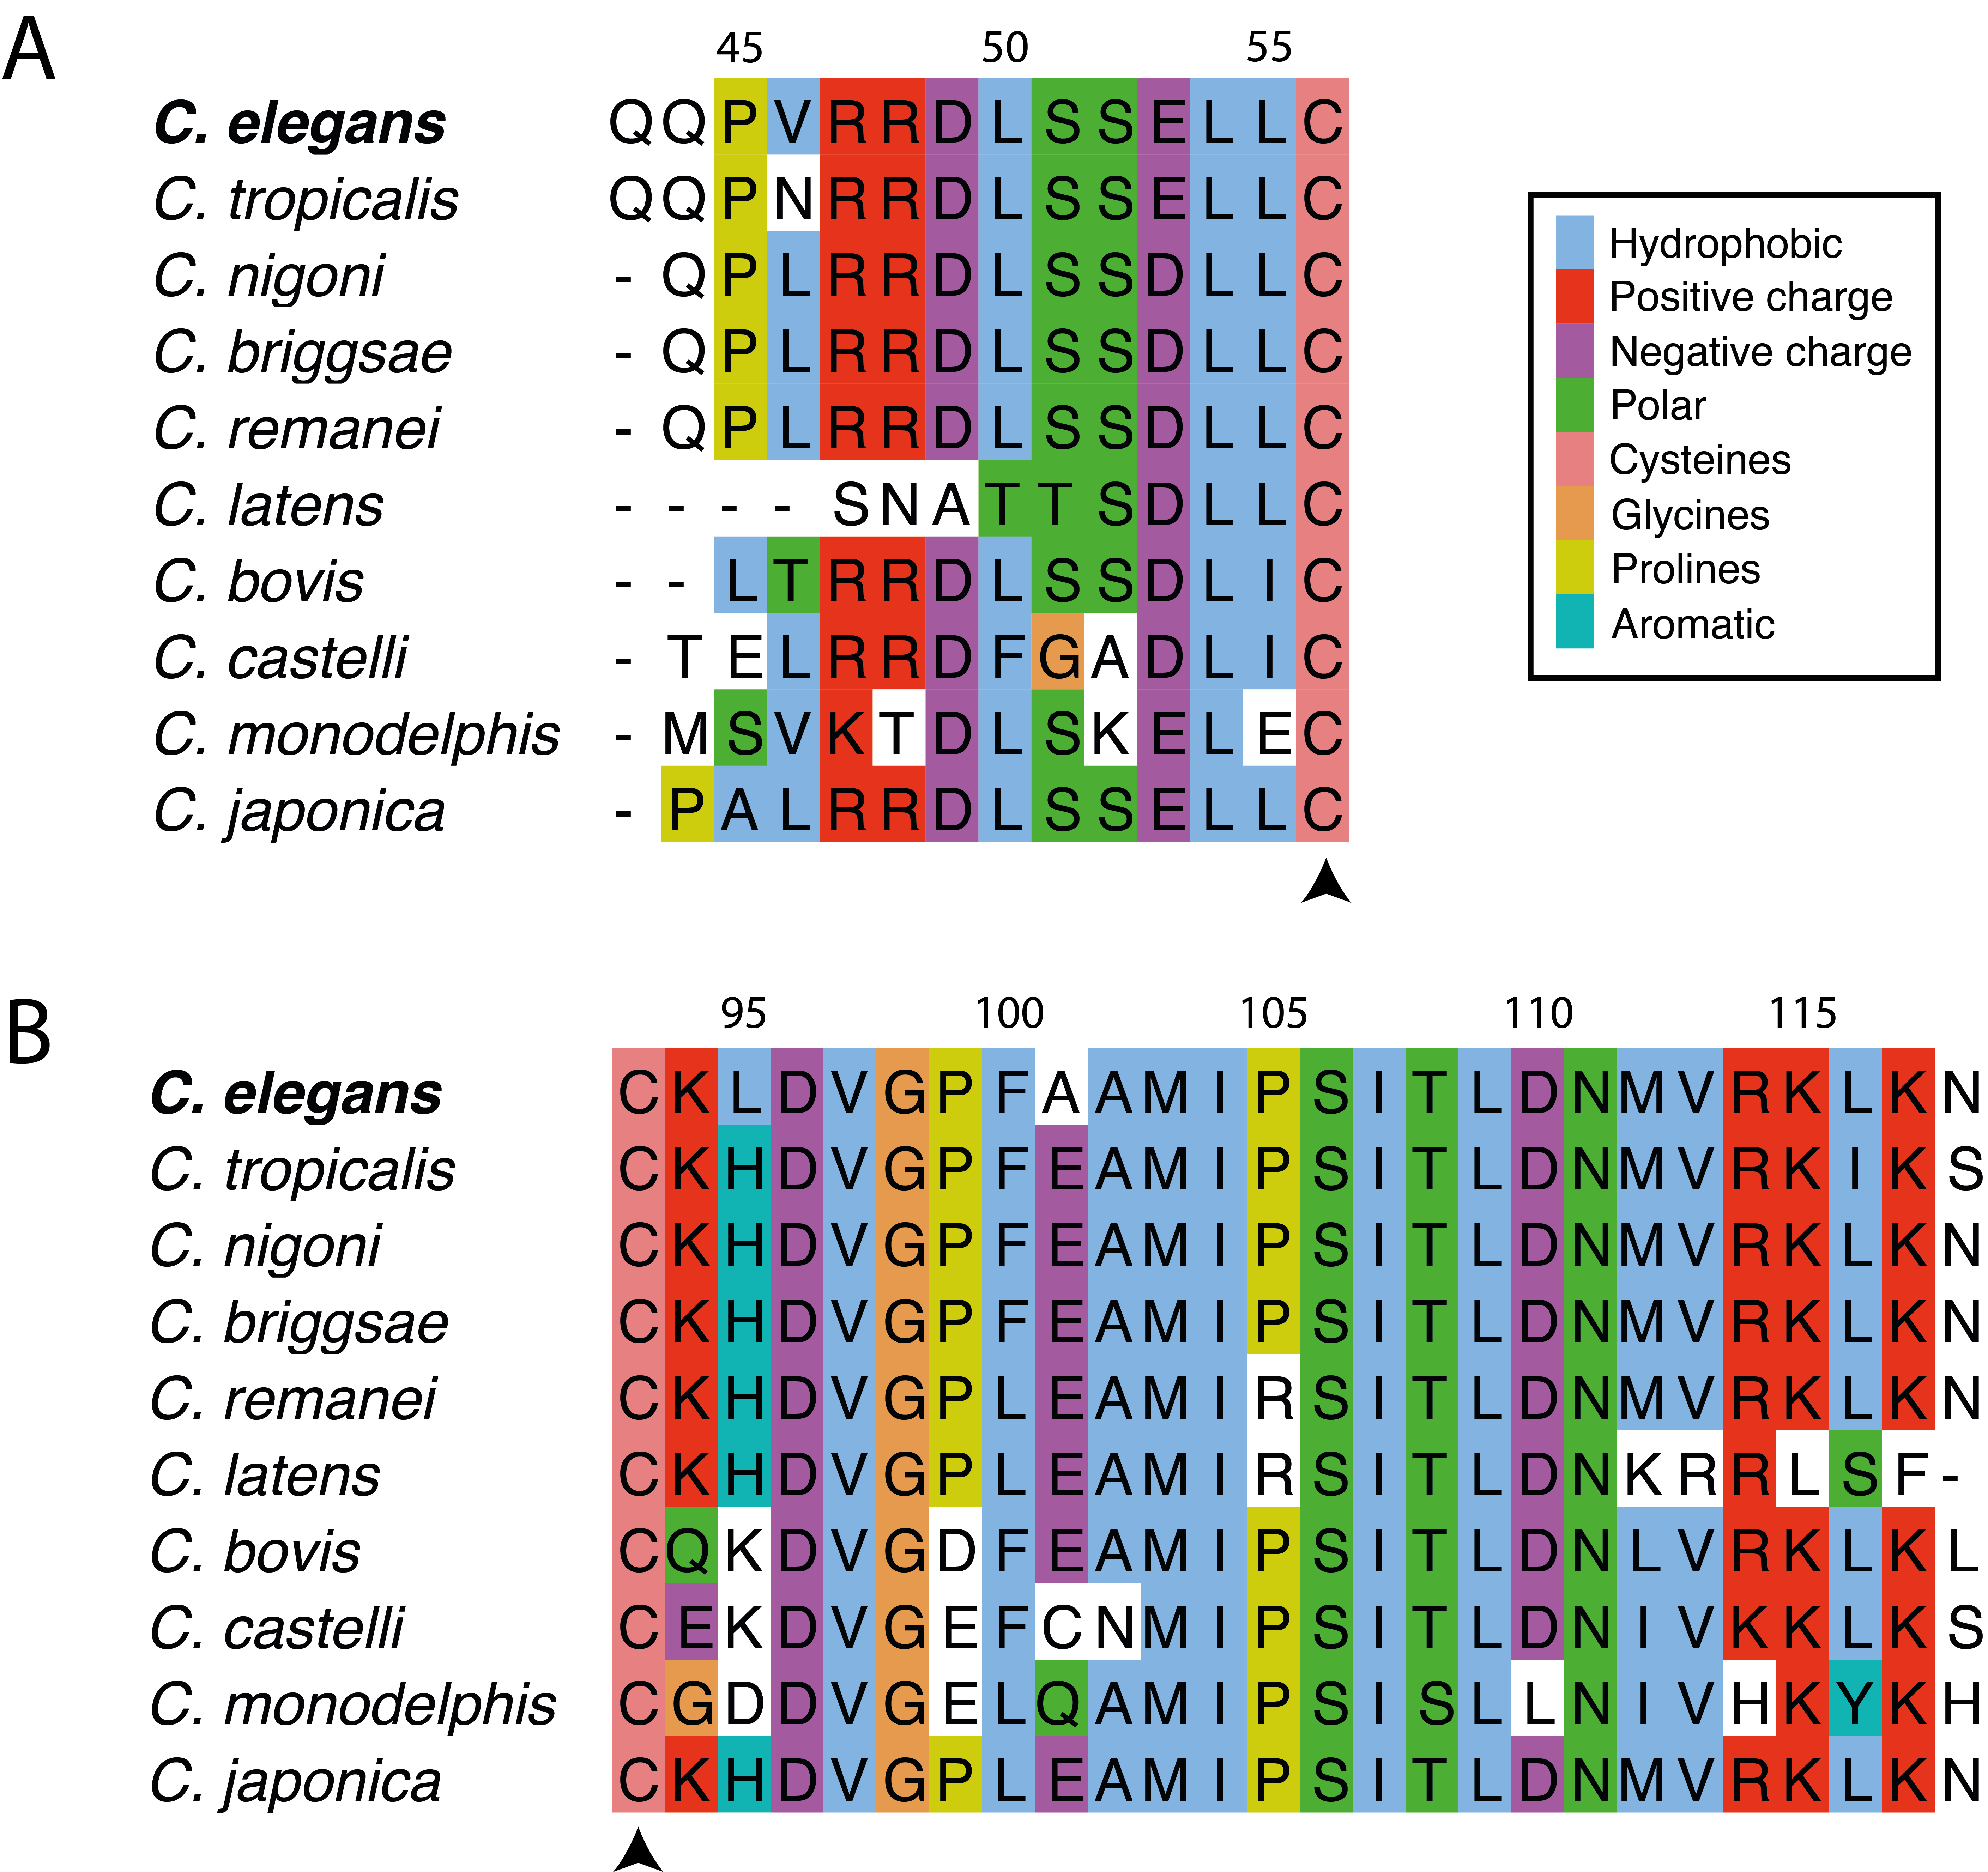
\includegraphics[scale=1]{alignments_par2}
\centering
\mycaption{Alignment of the PAR-2 RING domain N and C helices within the \textit{Caenorhabditis} genus}{
\textbf{(A)} N-helix alignment. Arrowhead indicates first zinc-coordinating cysteine of the core RING domain.
\textbf{(B)} C-helix alignment. Arrowhead indicates final zinc-coordinating cysteine of the core RING domain. Hydrophobic residues indicated in blue.
}
\label{fig:alignments_par2}
\end{figure}


\subsection{The PAR-2 RING domain displays concentration-dependent dimerisation in vitro}

The sequence analysis above suggests that the PAR-2 RING should likely have the ability to dimerise. To directly test this, we aimed to purify a fragment of PAR-2 containing the core RING domain and putative N and C helix regions (amino acids 40-120), and characterise its properties in vitro. We were successfully able to express the fragment in bacteria, and purify it by His pull down, followed by tag removal, ion exchange chromatography and size exclusion chromatography (see Methods).\\

To understand the oligomeric properties of the PAR-2 RING domain in solution, we subjected our purified sample to SEC-MALS, a common approach for characterising the molecular mass and oligomeric state of protein samples. The strategy follows a two step process. Firstly, size exclusion chromatography (SEC), separates particles in a sample based on their size. Larger particles leave the SEC column before smaller particles (i.e. at lower retention volumes). Refractive index scores monitor the concentration of particles leaving the column. Secondly, the eluent flow leaving the SEC column is monitored continuously by a multi-angle light scattering (MALS) instrument, which provides an estimate of the molecular weight of particles based on light scattering properties.\\

We performed five SEC-MALS assays on PAR-2 RING, using sample concentrations of 10, 5, 2, 0.75 and 0.5 mg/ml (\cref{fig:sec_mals}A). In all cases a single peak is observed in refractive index traces, with corresponding molar mass measurements by MALS somewhere between the expected weight of a monomer and a dimer, suggesting that the sample exists in a monomer-dimer equilibrium. Furthermore, mass distributions show clear concentration-dependence, with more concentrated samples giving higher molar mass measurements. This is more clearly visualised in \cref{fig:sec_mals}B, which shows that the average molecular weight of particles in the sample increases as a function of sample concentration.  Comparison to a dimerisation model (black line) shows a good fit. Overall, this data suggests that the PAR-2 RING domain displays concentration-dependent dimerisation, existing largely as a monomer at low concentrations and mostly dimeric at higher concentrations.\\

\begin{figure}
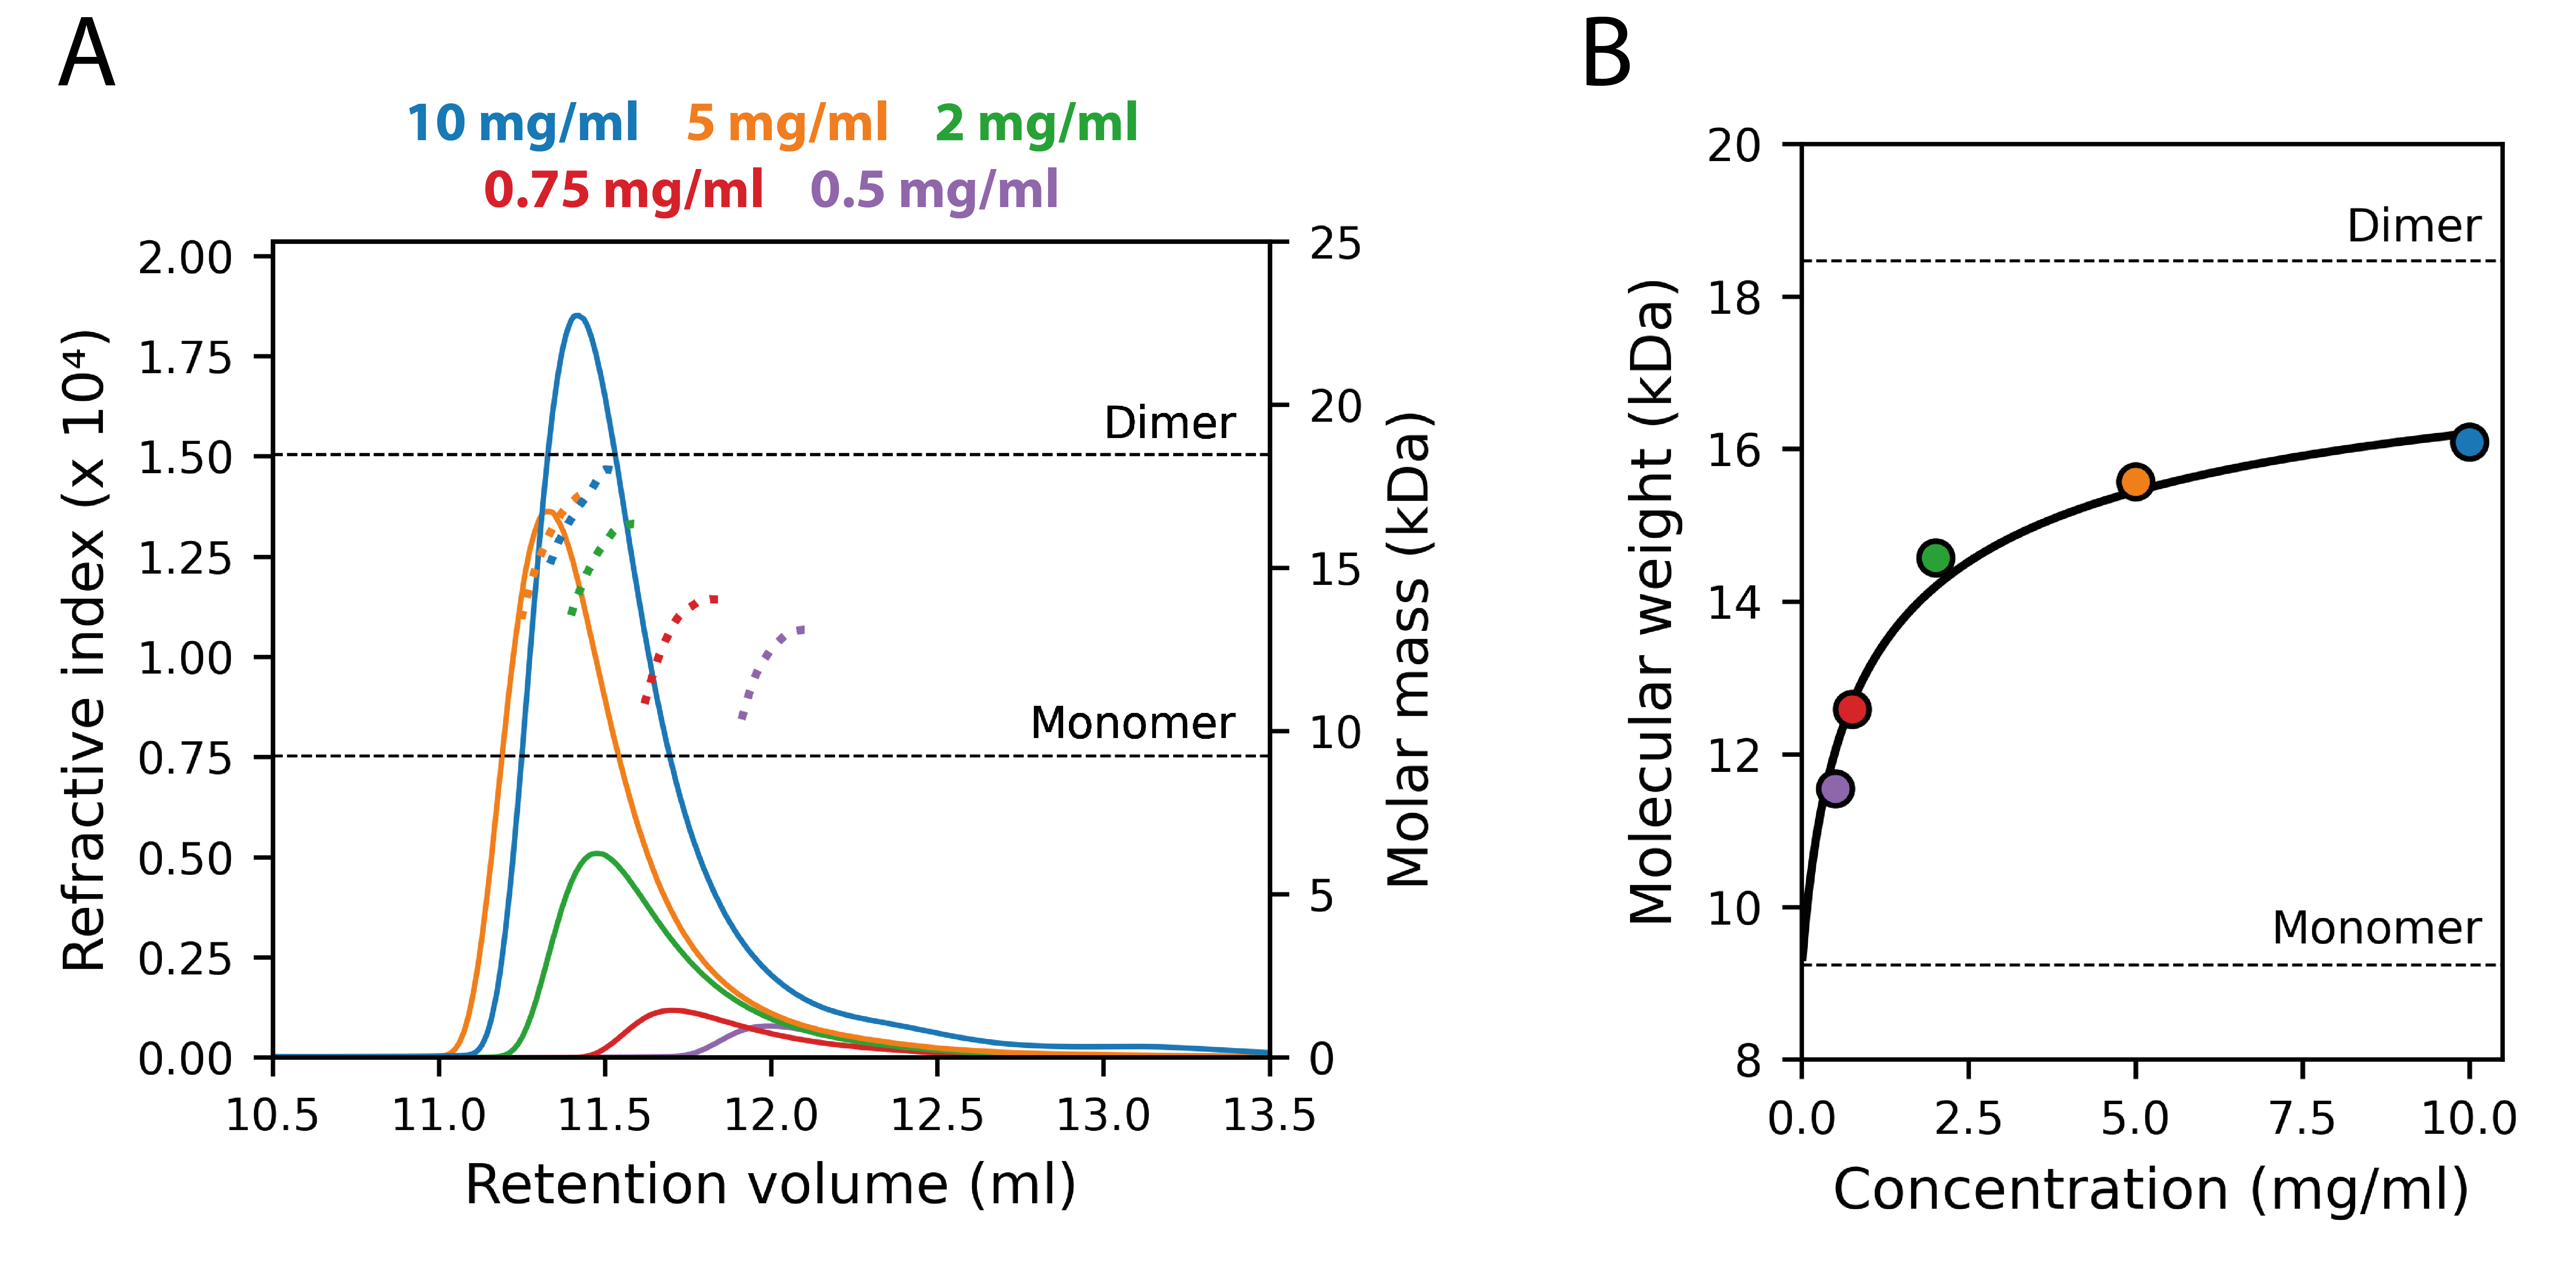
\includegraphics[scale=1]{sec_mals_v2}
\centering
\mycaption{SEC-MALS titration reveals concentration-dependent dimerisation of the PAR-2 RING domain}{
\textbf{(A)} SEC-MALS traces for the PAR-2 RING domain at different concentrations. Solid lines indicate refractive index measurements, dotted lines indicate molar mass measurements. Colour coded by sample concentration. Note that effective concentrations are lower than this as sample gets diluted in the instrument. MALS traces are cropped to retention volumes for which refractive index is $>$ 80\% of its peak value.
\textbf{(B)} Weight-average molecular weight measurements vs. sample concentration for the SEC-MALS assays in (A). Solid line indicates fit to a dimerisation model.
}
\label{fig:sec_mals}
\end{figure}


\subsection{Dimerisation is mediated by 4-helix bundle with hydrophobic core}

To better understand the structural basis of dimerisation, we aimed to resolve the structure of the PAR-2 RING domain dimer by X-ray crystallography. We successfully purified sufficient quantities of protein to set up crystal screens, but have so far been unsuccessful in generating crystals. Nevertheless, owing to recent advances in protein structure prediction tools, such as AlphaFold \citep{Jumper2021} and AlphaFold-Multimer \citep{Evans2022}, we can get good estimates of the protein structures based on their sequence of amino acids.\\

I used AlphaFold-Multimer to predict the structure of the PAR-2 RING domain dimer (residues 40-120 of the protein). The predicted structure (\cref{fig:ring_alphafold}) resembles the common structure of RING domain dimers, characterised by a four-helix bundle consisting of an N and C helix from each of the two monomers (\cref{fig:ring_alphafold}B). Within this bundle, we see a characteristic pattern of inwards facing hydrophobic residues (\cref{fig:ring_alphafold}D). Confidence scores, as measured by the AlphaFold metric pLDDT (predicted local distance difference test), are high throughout the structured region of the model (\cref{fig:ring_alphafold}C).\\


\begin{figure}
\includegraphics[scale=0.9]{ring_alphafold}
\centering
\mycaption{AlphaFold prediction for the 3D structure of the PAR-2 RING domain dimer}{
\textbf{(A)} 3D structure colour coded by chain.
\textbf{(B)} 3D structure with N and C helices highlighted.
\textbf{(C)} 3D structure colour coded by pLDDT, an AlphaFold metric for prediction confidence.
\textbf{(D)} 3D structure colour coded by hydrophobicity, with red indicating more hydrophobic and white indicating less hydrophobic. Inset shows enlarged view of the 4-helix bundle, showing internally facing hydrophobic residues.
}
\label{fig:ring_alphafold}
\end{figure}

I also generated predictions for the PAR-2 RING across the \textit{Caenorhabditis} genus (\cref{fig:ring_alphafold_species}). These show that the 4-helix bundle structure is predicted to be conserved across the genus, although prediction confidence scores within this region are variable.\\

\begin{figure}
\includegraphics[scale=0.9]{ring_alphafold_species}
\centering
\mycaption{AlphaFold predictions for the PAR-2 RING domain across the \textit{Caenorhabditis} genus}{
Colour coded by pLDDT.
}
\label{fig:ring_alphafold_species}
\end{figure}

Given that dimerisation is predicted to be mediated by a hydrophobic interface within a 4-helix bundle, we would expect that mutations to hydrophobic residues within this region should disrupt dimerisation, as has been shown previously for several RING domains \citep{Koliopoulos2016, Rojas-Fernandez2014, Liew2010}. Unlike mutations to zinc-coordinating cysteines, which completely misfold the domain, mutations to this interface should preserve the tertiary structure of the domain and specifically disrupt dimerisation. I identified L109, predicted to be found in the C-helix, as a likely important site (\cref{fig:l109r_sec_mals}A), and L109R as a likely disruptive mutation. As we did for the wild-type RING domain, we expressed the mutant allele in bacteria and purified it using the same protocol. SEC-MALS shows that this mutant has the expected molecular weight of a predominantly monomeric population (\cref{fig:l109r_sec_mals}B, C). By contrast, wild type RING at an equivalent concentration (\cref{fig:sec_mals}A, 0.75 mg/ml) is partially dimeric (\cref{fig:l109r_sec_mals}C). We cannot rule out that PAR-2(L109R) dimerises at higher concentrations, but were unable to purify sufficient quantities to test at higher levels.\\

\begin{figure}
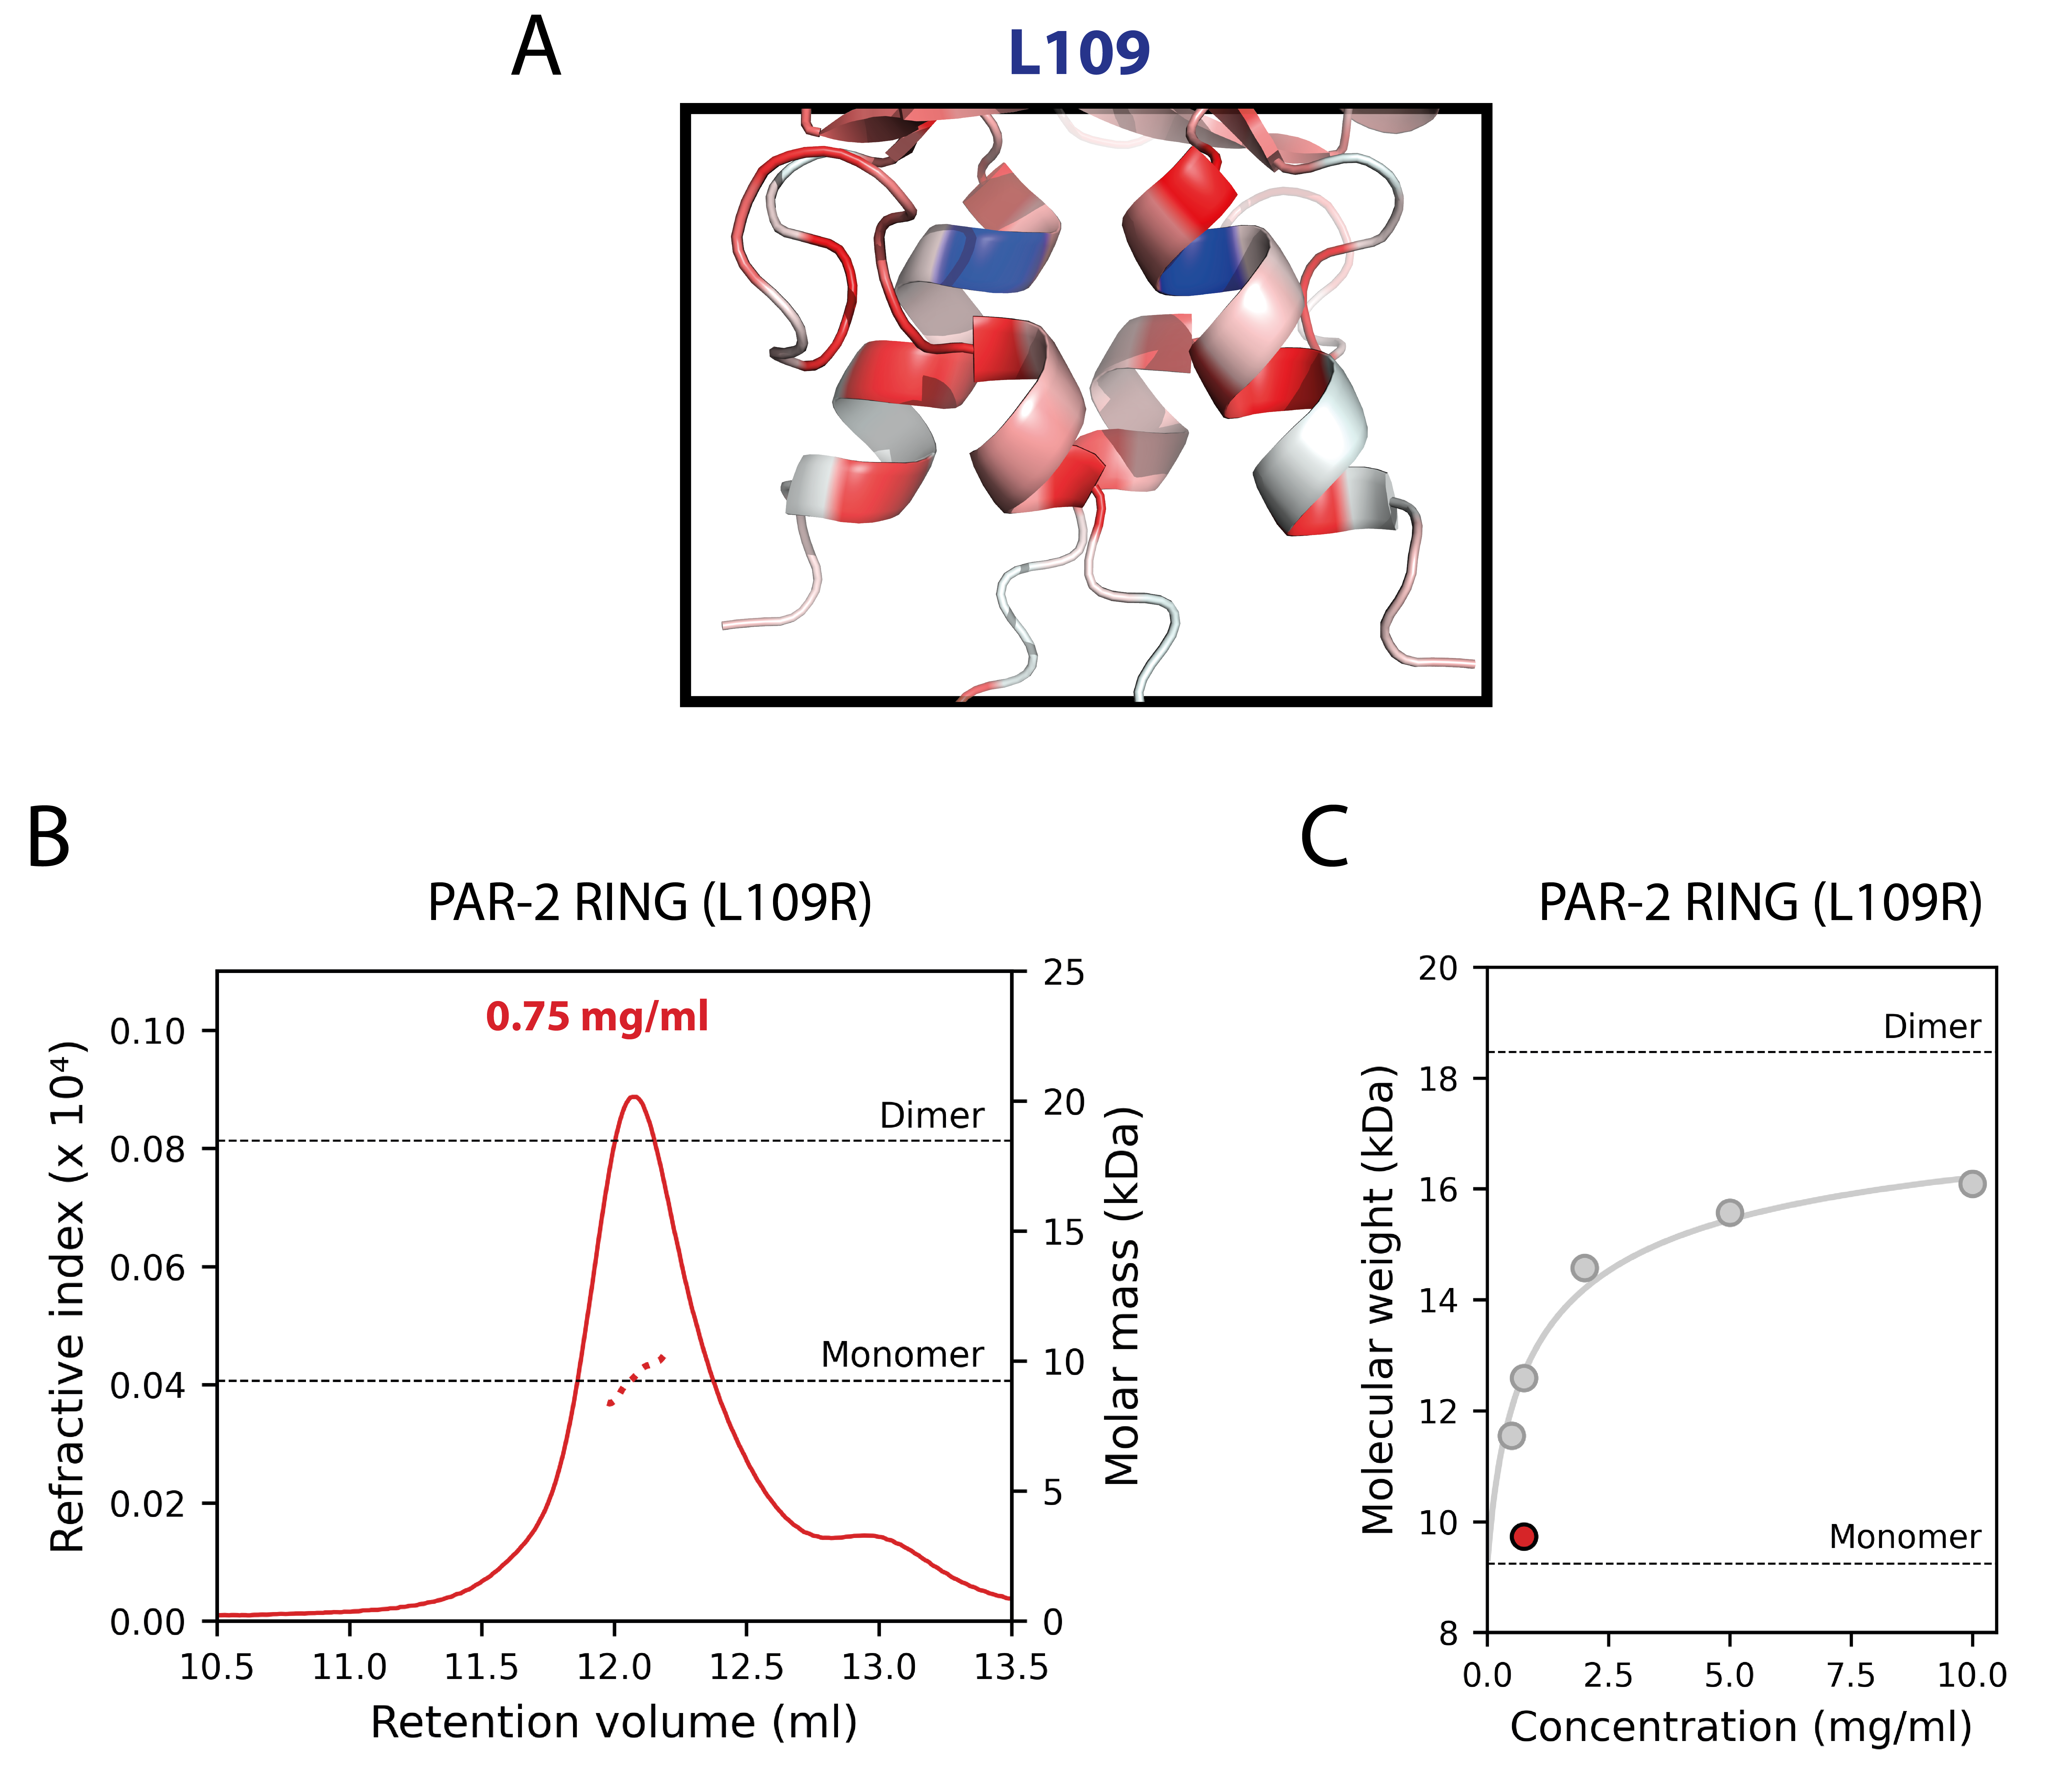
\includegraphics[scale=1]{l109r_sec_mals_v2}
\centering
\mycaption{Mutation of residue at hydrophobic interface disrupts PAR-2 RING domain dimerisation}{
\textbf{(A)} Position of the L109 site within the 4-helix bundle of the PAR-2 RING domain dimer (AlphaFold prediction). L109 site highlighted in blue, other residues coloured by hydrophobicity.
\textbf{(B)} SEC-MALS trace for PAR-2 RING (L109R). Solid line indicates refractive index, dotted line indicates molar mass. Sample concentration 0.75 mg/ml.
\textbf{(C)} Weight-average molecular weight vs. sample concentration for the single SEC-MALS trace in (B). Shown against wild-type data (gray).
}
\label{fig:l109r_sec_mals}
\end{figure}

As a further test, we attempted to express and purify a C56S mutant RING domain for SEC-MALS. However, we found the protein to be unstable in vitro and were unable to purify it significant quantities to perform the assay, which is a common problem for unfolded proteins.\\

\subsection{Cytoplasmic PAR-2 does not self-associate in vivo}

The in vitro results described so far suggest that the PAR-2 RING domain displays concentration-dependent dimerisation. In vivo, PAR-2 concentrations are relatively low in the cytoplasm, but local concentrations are greatly enhanced upon membrane association. To investigate the potential role for RING-mediated PAR-2 dimerisation in vivo, I considered the cytoplasmic and membrane fractions separately, and devised two in vivo assays designed to test for the ability of PAR-2 to self-associate in the cytoplasm and on the membrane.\\

To test for self-association of cytoplasmic PAR-2, I devised an in vivo pull-down assay based on dual labelling of PAR-2 with two different fluorophores (\cref{fig:tomm20_schematic}). Expressing PAR-2 with a mix of GFP and mCherry fluorophores means that, were cytoplasmic PAR-2 to form dimers, a mixed population of GFP/GFP, GFP/mCherry and mCherry/mCherry dimers would be expected to be present within the cytoplasm. Thus, forced relocalisation of GFP::PAR-2 to a particular location in the cell should result in a detectable signal mCherry::PAR-2 at that location. A similar assay was used previously by \textcite{Reich2019}, who demonstrated a stable interaction between PAR-6 and PKC-3 through forced localisation of GFP::PKC-3 to the plasma membrane with a plasma membrane tethered GFP binding protein (GBP). (In this case the plasma membrane was a suitable target because, under the conditions of that particular assay, PAR-6/PKC-3 do not normally bind to the plasma membrane). Here, I propose a similar approach, relying instead on recruitment to mitochondrial membranes within the cell. Mitochondrial membranes are dense within the \textit{C. elegans} zygote \citep{Dinkelmann2003}, and can be probed easily with a localisation signal from the TOMM-20 protein \citep{Watanabe2011}.\\

\begin{figure}
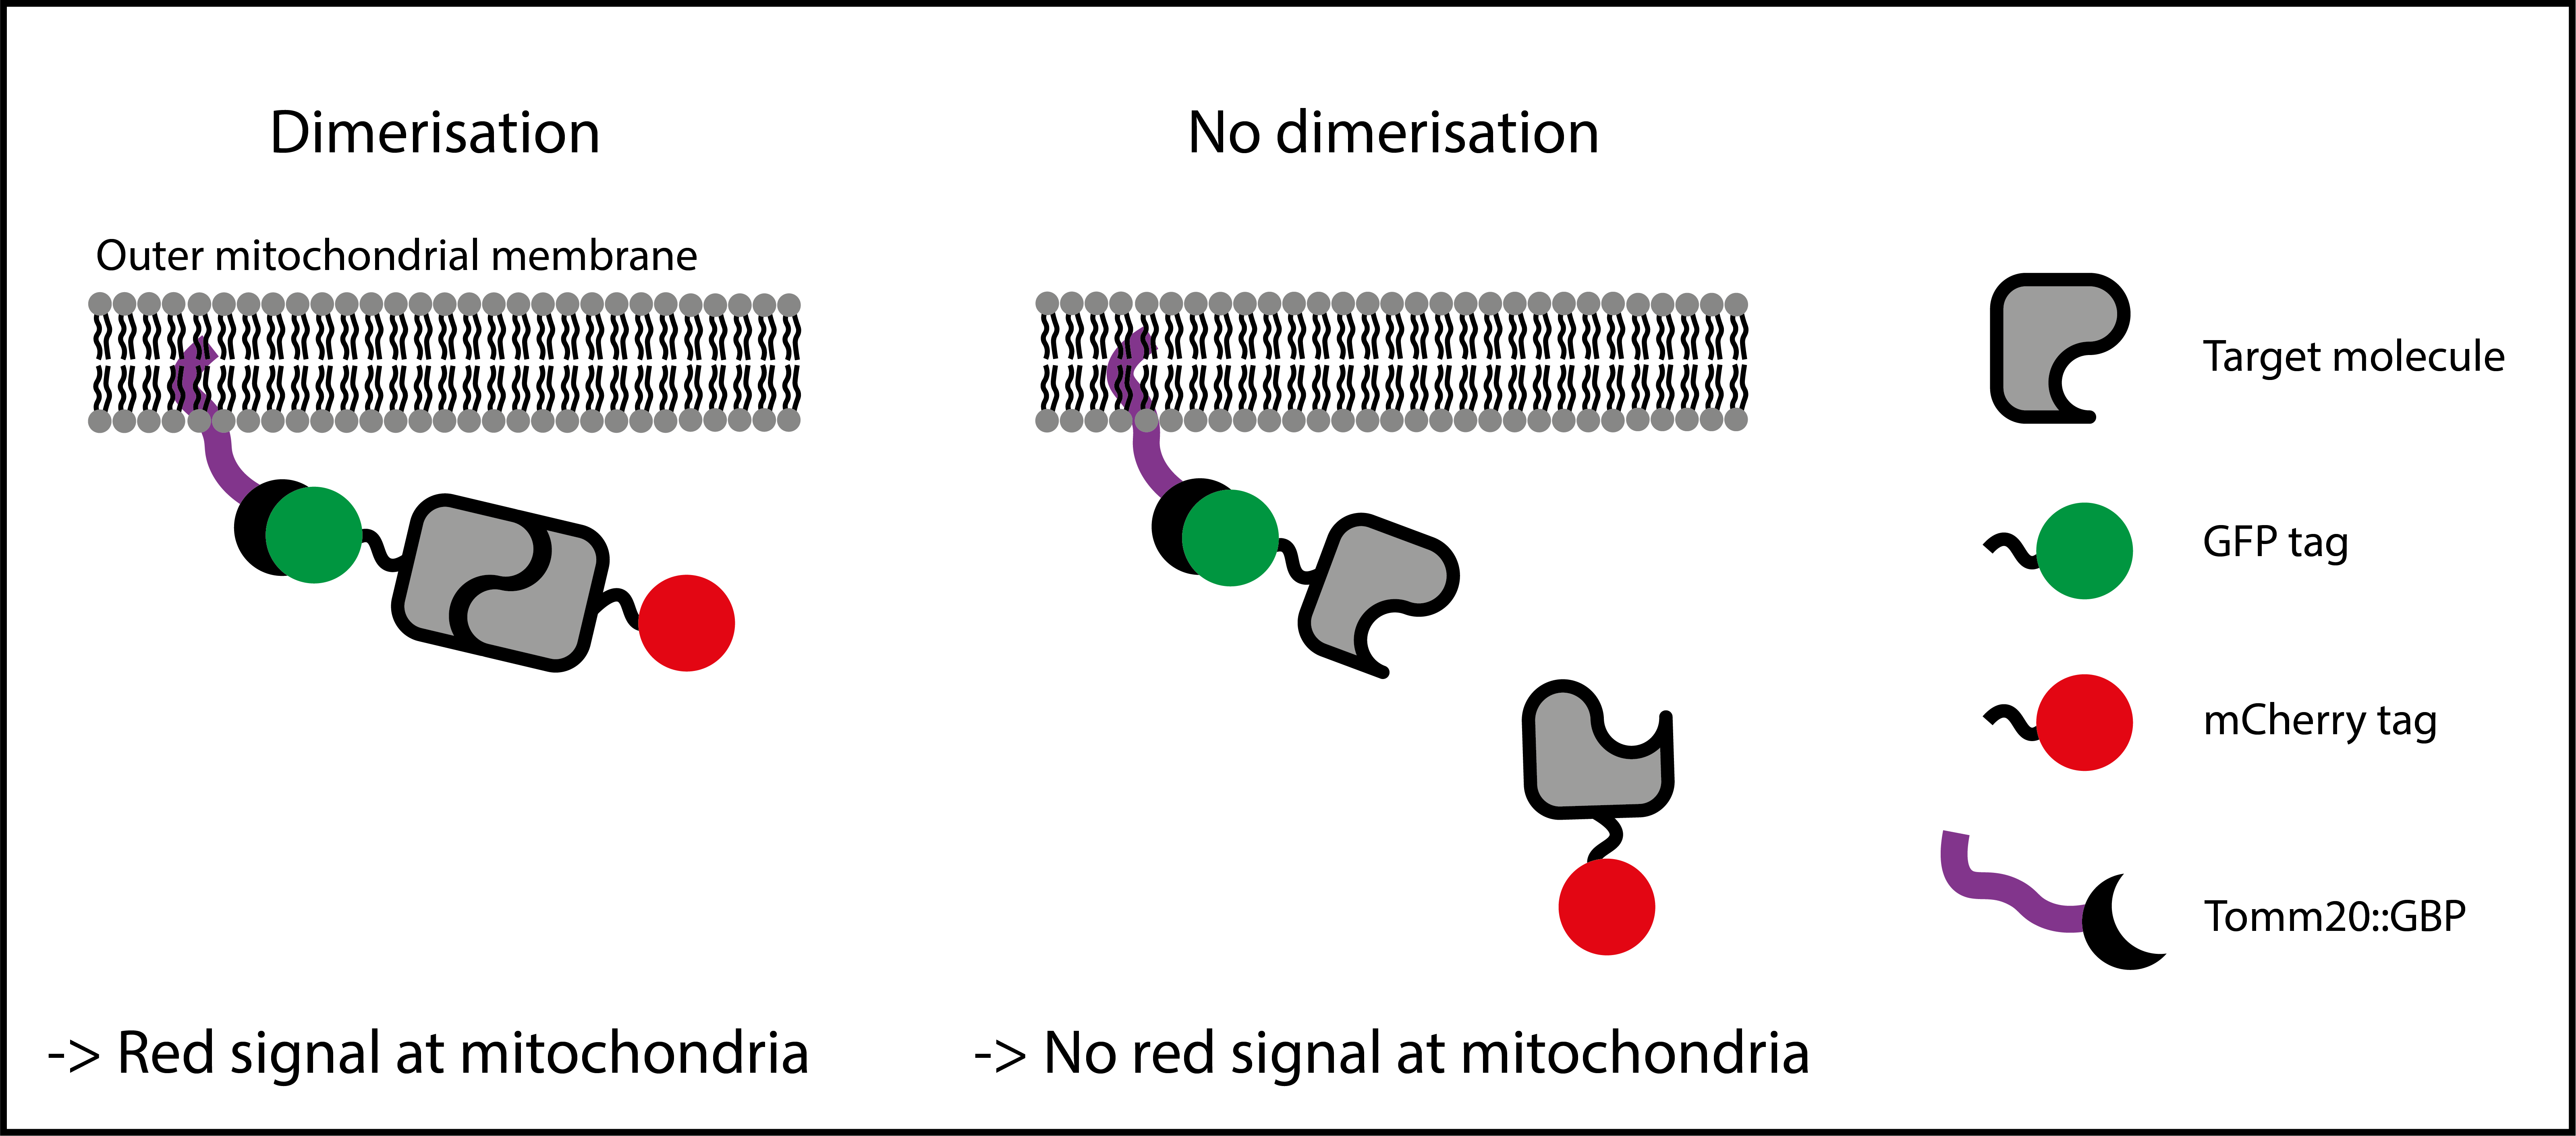
\includegraphics[scale=0.95]{tomm20_schematic}
\centering
\mycaption{Schematic of an in vivo dimerisation assay involving the mitochondrial probe TOMM-20}{
}
\label{fig:tomm20_schematic}
\end{figure}

To first test the potential utility of this method, I built a TOMM-20::GBP probe tagged with mKate, and introduced this into the worm by CRISPR. Crossing this line to a GFP::PAR-2 expressing line, and imaging the F1s (heterozygous for both GFP::PAR-2 and the probe), shows that the probe is well expressed, displays the expected mitochondrial localisation pattern, and is able to recruit GFP::PAR-2 to the mitochondria (\cref{fig:tomm20_merge}).\\

\begin{figure}
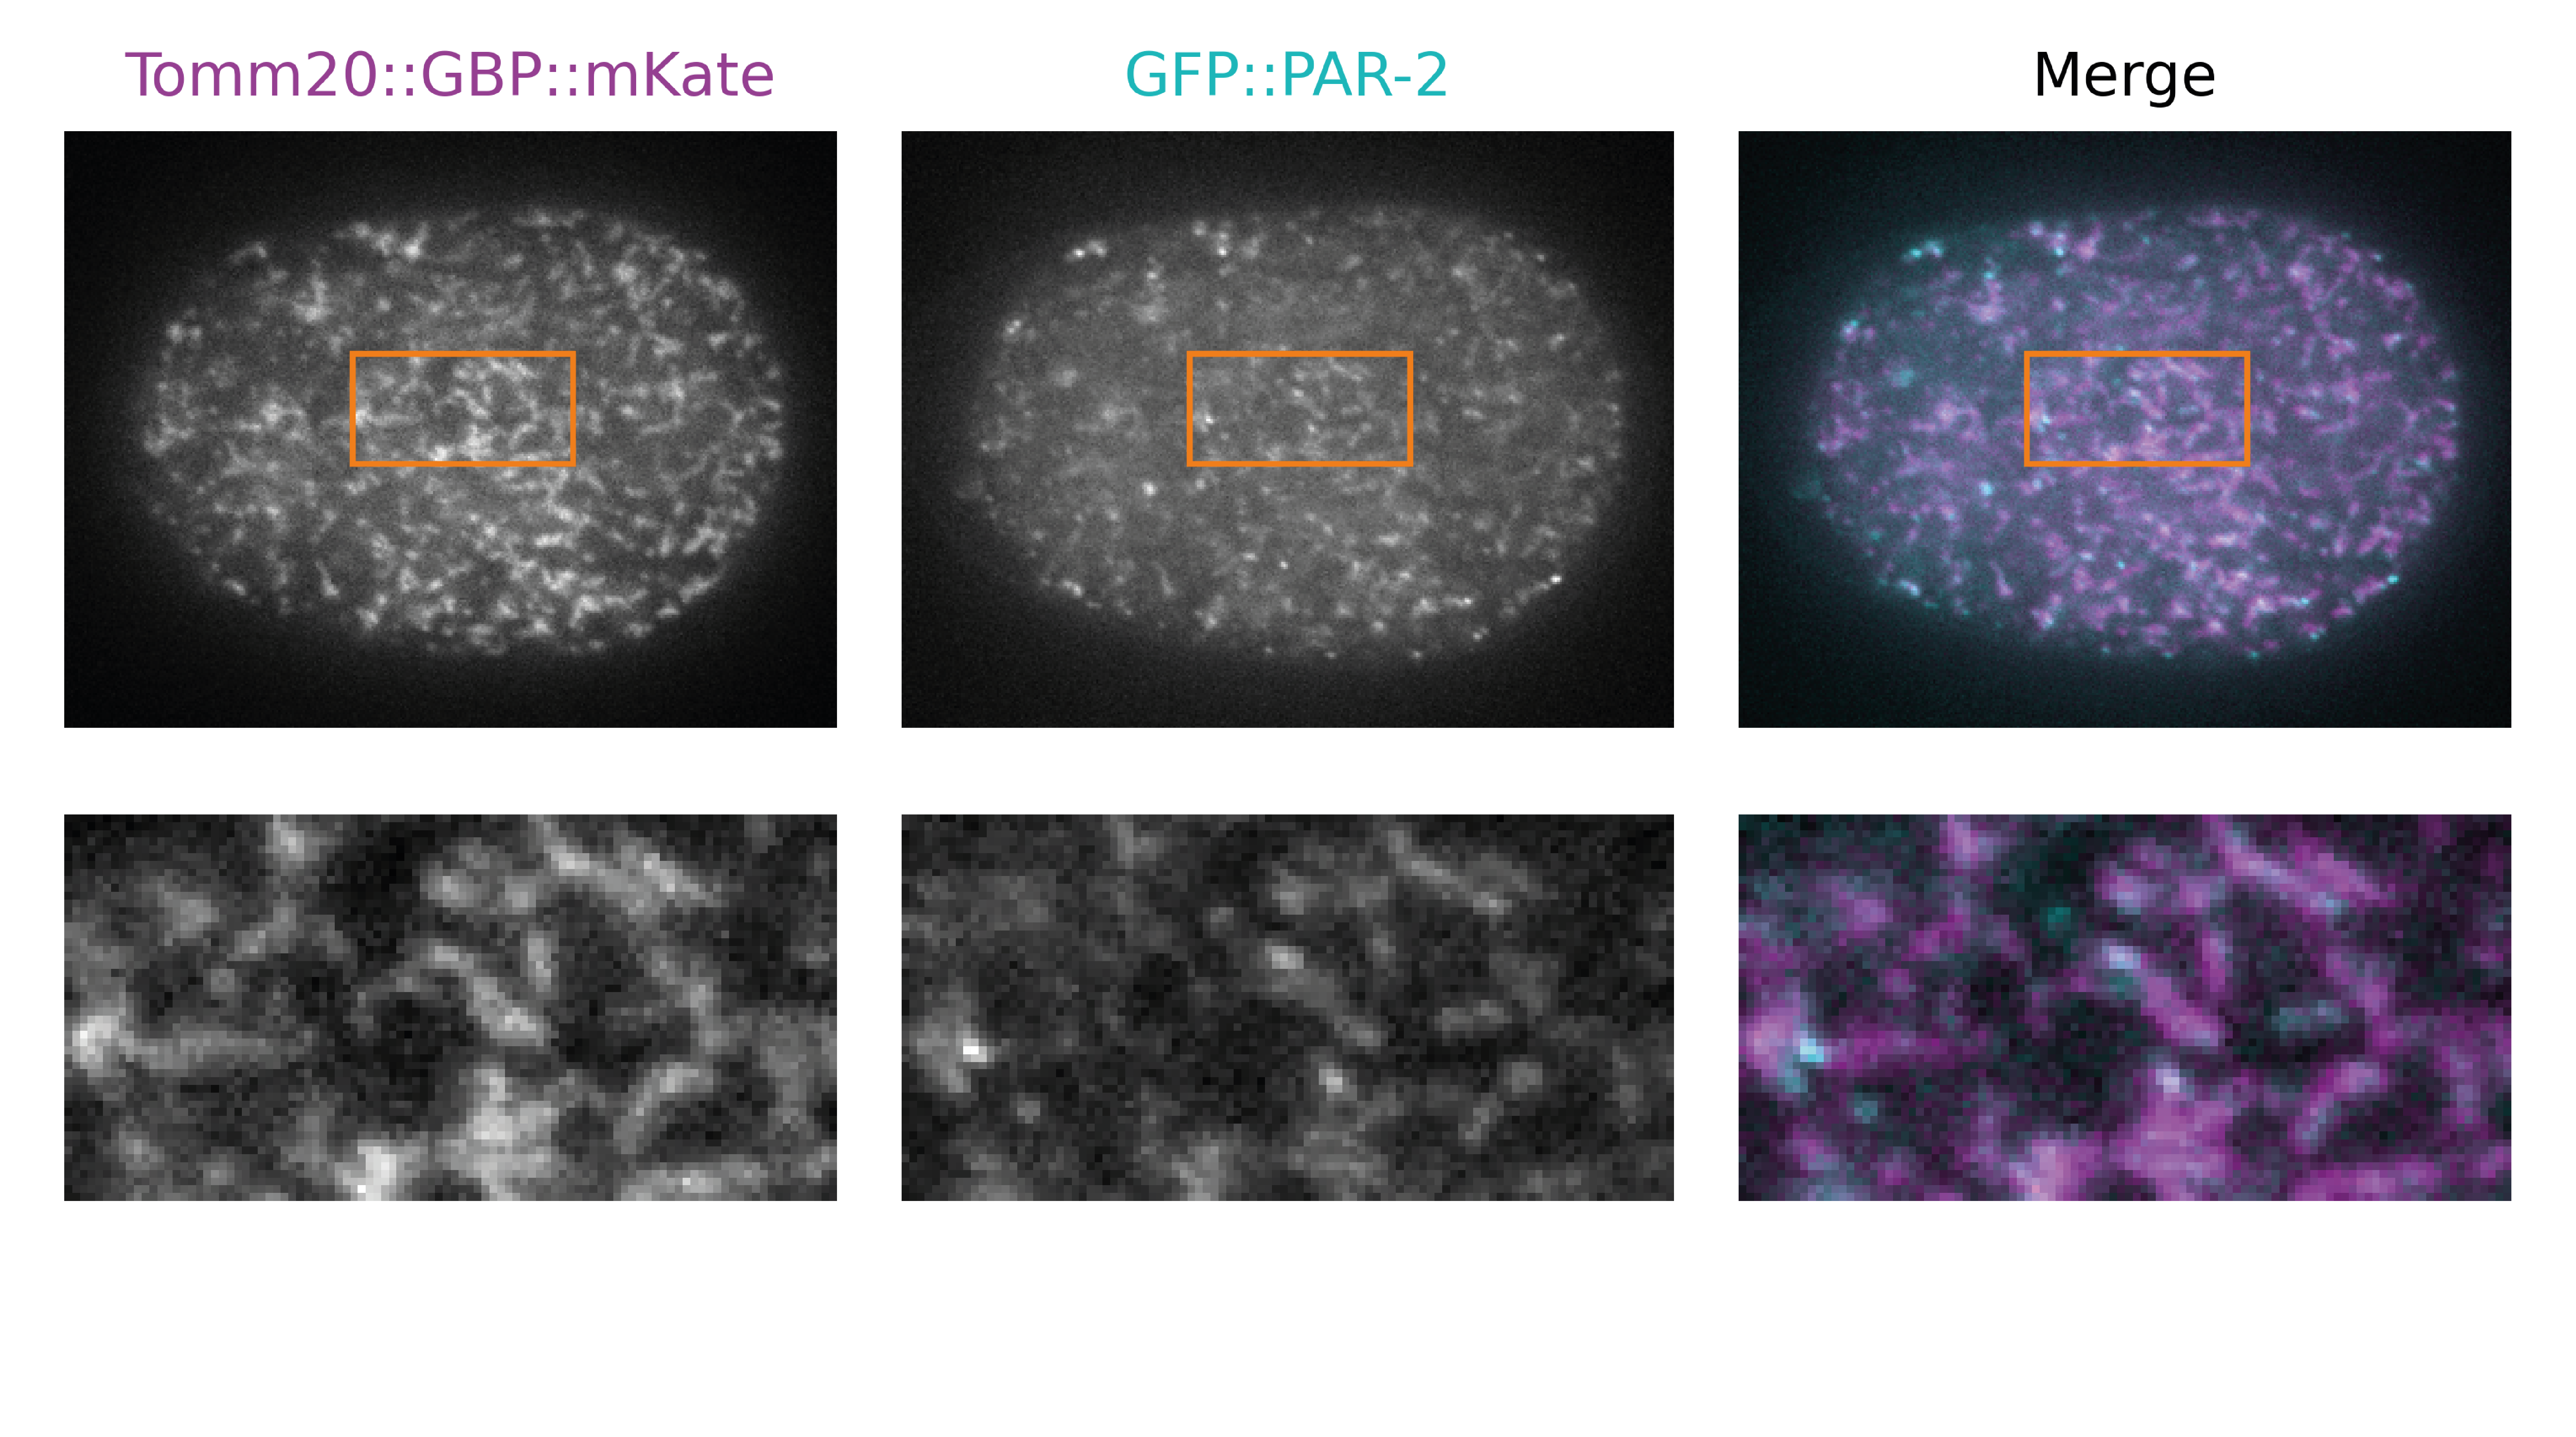
\includegraphics[scale=0.95]{tomm20_merge}
\centering
\mycaption{Mitochondrial GFP nanobody pulls GFP-tagged PAR-2 to mitochondria}{
Images of a zygote expressing Tomm20::GBP::mKate and GFP::PAR-2.
GFP channel image is not autofluorescence corrected. Shows a view between the midplane and cortex, as this gives a clearer signal for mitochondria.
}
\label{fig:tomm20_merge}
\end{figure}

To perform the proposed two-colour dimerisation assay, I next attempted to build an untagged version of the mitochondria probe (lacking mKate). Whilst I was successfully able to introduce the construct into the genome of the worm, I found that this untagged probe failed to recruit any GFP::PAR-2 to the mitochondria, likely indicating that the probe failed to express. This suggests that the mKate tag may be stabilising expression of the full construct, possibly due to the presence of introns within the mKate sequence. As an alternative method to free up the red channel, I introduced a point mutation into mKate by CRISPR designed to disrupt the chromophore region, which is required for fluorescence \citep{Pletnev2008}. This construct, by contrast, was well expressed and, like the tagged parent construct, able to pull GFP::PAR-2 to the mitochondria. Next, I crossed this line to a line expressing mCherry::PAR-2 at the endogenous locus, homozygosing both constructs. I then crossed the resulting line to a line homozygous for endogenous GFP::PAR-2, giving F1s heterozygous for GFP/mCherry PAR-2, and heterozygous for the mitochondrial probe. Imaging embryos from these F1s showed that, whereas GFP::PAR-2 is fully pulled to the mitochondria, there is no detectable colocalisation with mCherry::PAR-2, which retains a normal pattern of cytoplasmic and cortical localisation (\cref{fig:tomm20_assay}). Overall, as mCherry signal is not observed at the mitochondria, the result implies that cytoplasmic PAR-2 is largely or entirely monomeric.\\

\begin{figure}
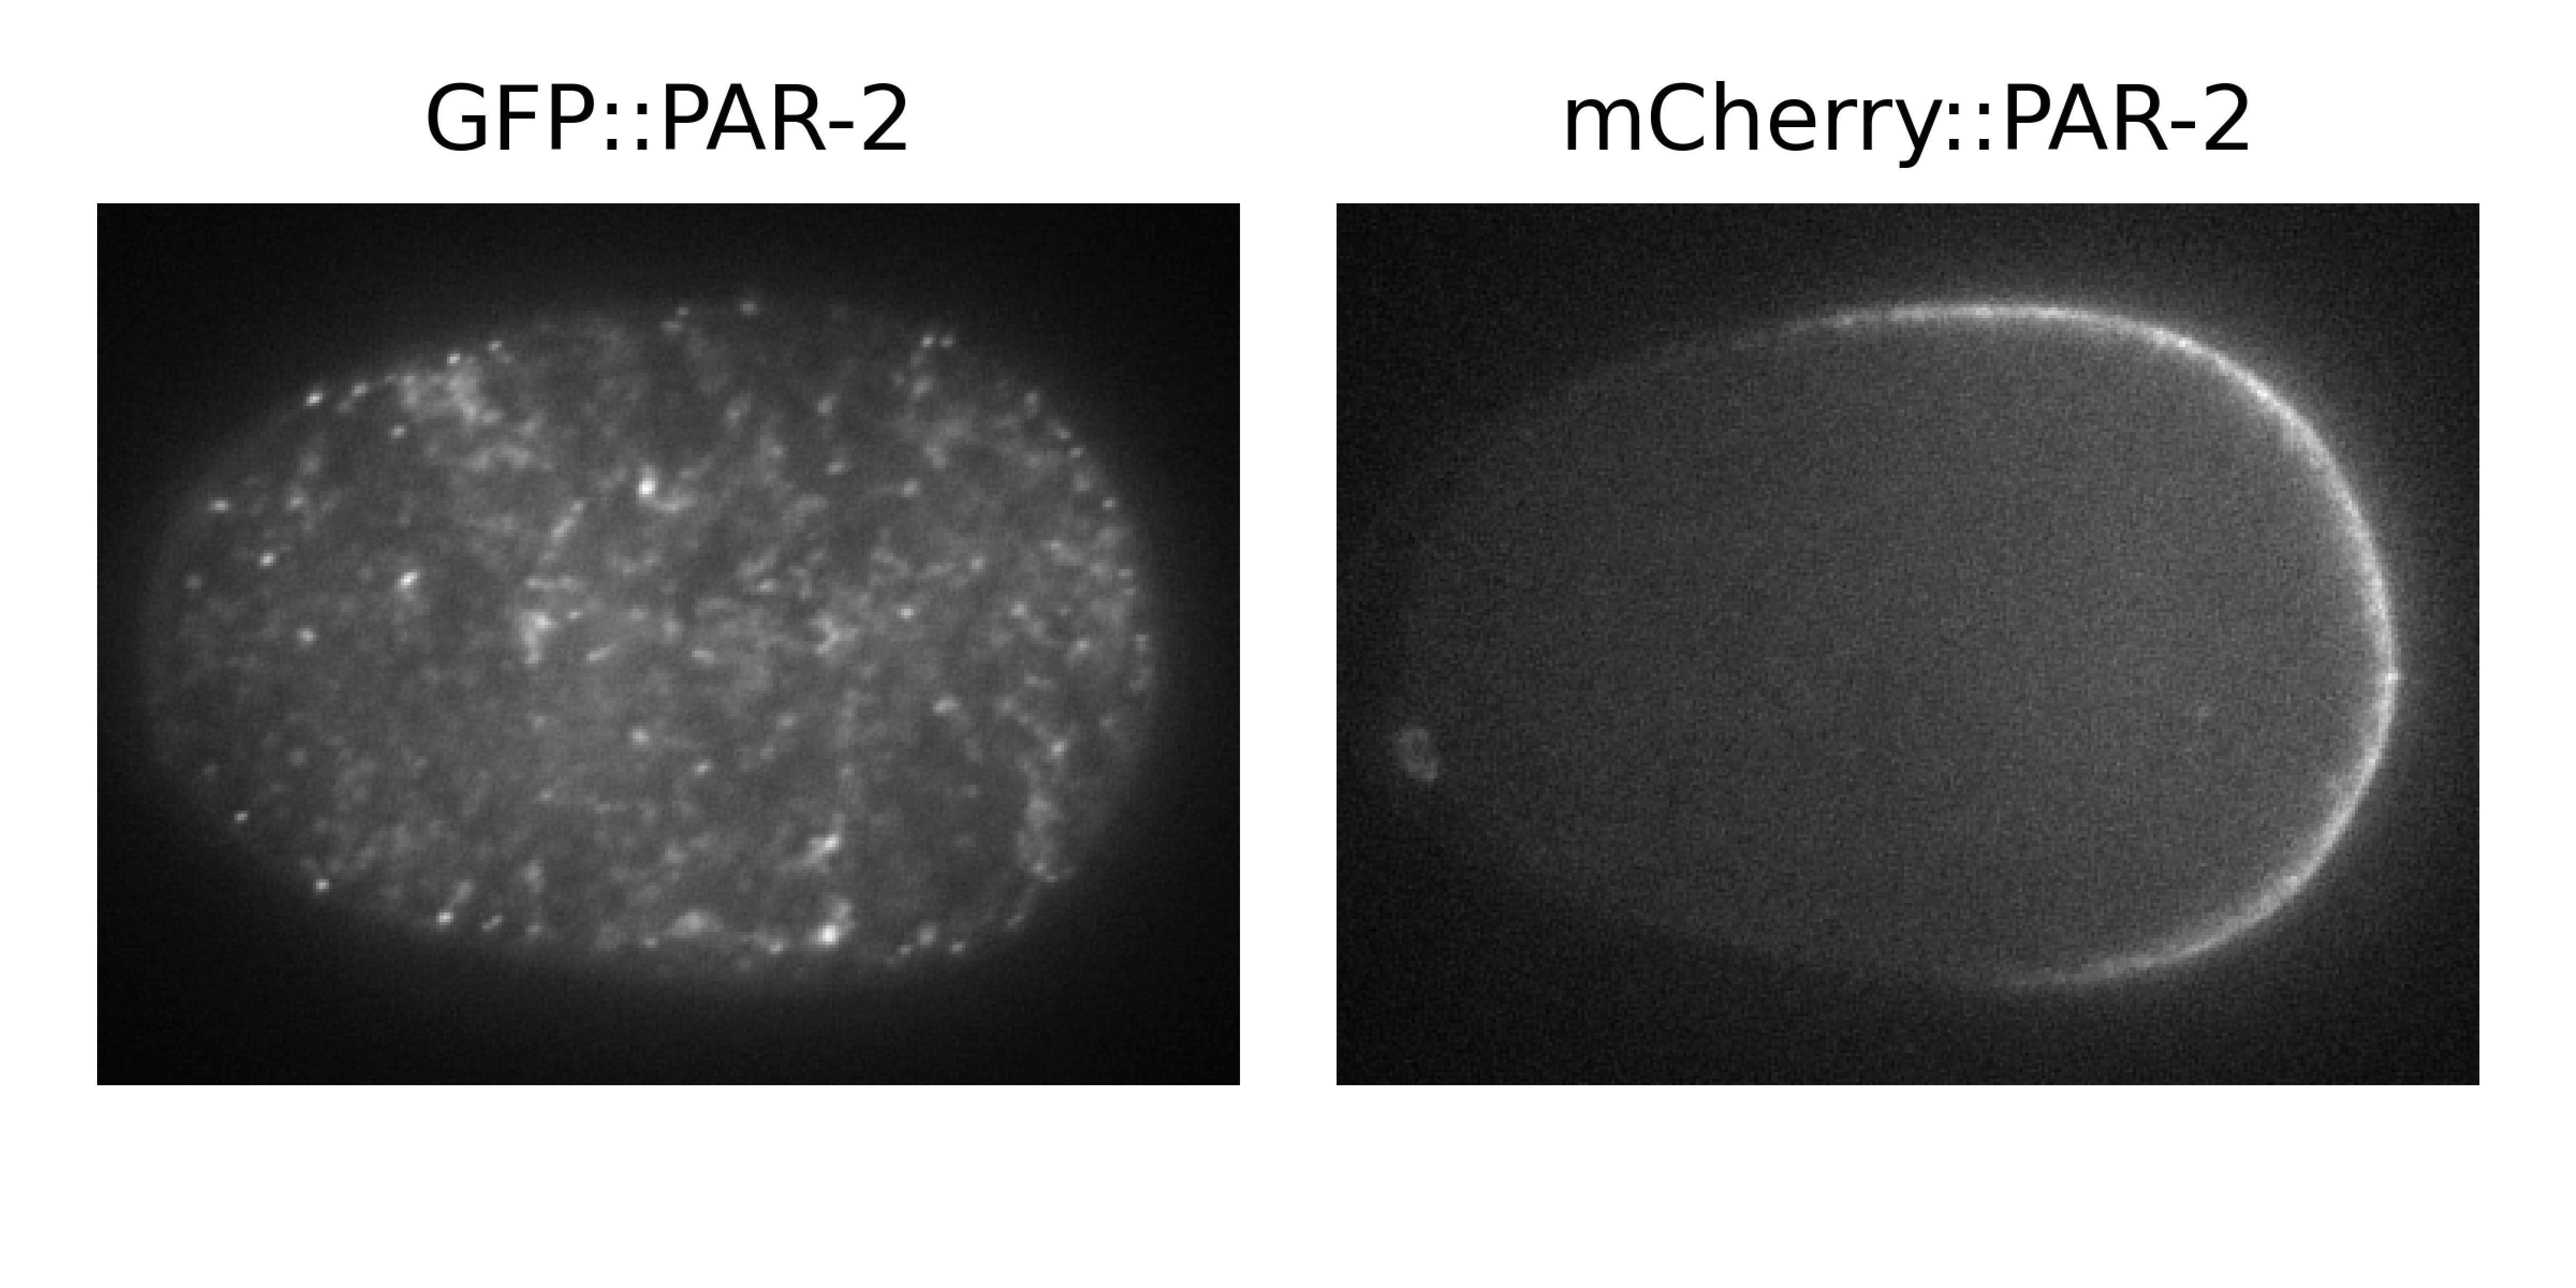
\includegraphics[scale=1]{tomm20_assay}
\centering
\mycaption{In vivo dimerisation assay shows that PAR-2 does not constitutively dimerise in vivo}{
Images of GFP::PAR-2 and mCherry::PAR-2 in a line heterozygous for GFP/mCherry PAR-2 and heterozygous for TOMM-20::GBP. GFP channel image is not autofluorescence corrected. Shows a view between midplane and cortex as this gives a clearer signal for mitochondria.
}
\label{fig:tomm20_assay}
\end{figure}


\subsection{Membrane-enriched PAR-2 self-associates in vivo}

I next aimed to test the ability of the PAR-2 RING to dimerise on the membrane, where concentrations are greatly enhanced compared to the cytoplasm. A RING-containing fragment of PAR-2 (1-177) expressed on its own as an exogenous construct fails to localise to the plasma membrane (\cref{fig:ring_fragment_in_vivo} and \cite{Hao2006}), indicating that this construct cannot dimerise with membrane-bound PAR-2. However, this does not account for the possibility that plasma membrane recruitment might first be required to permit dimerisation with endogenous PAR-2, perhaps by increasing effective local concentrations.\\

\begin{figure}
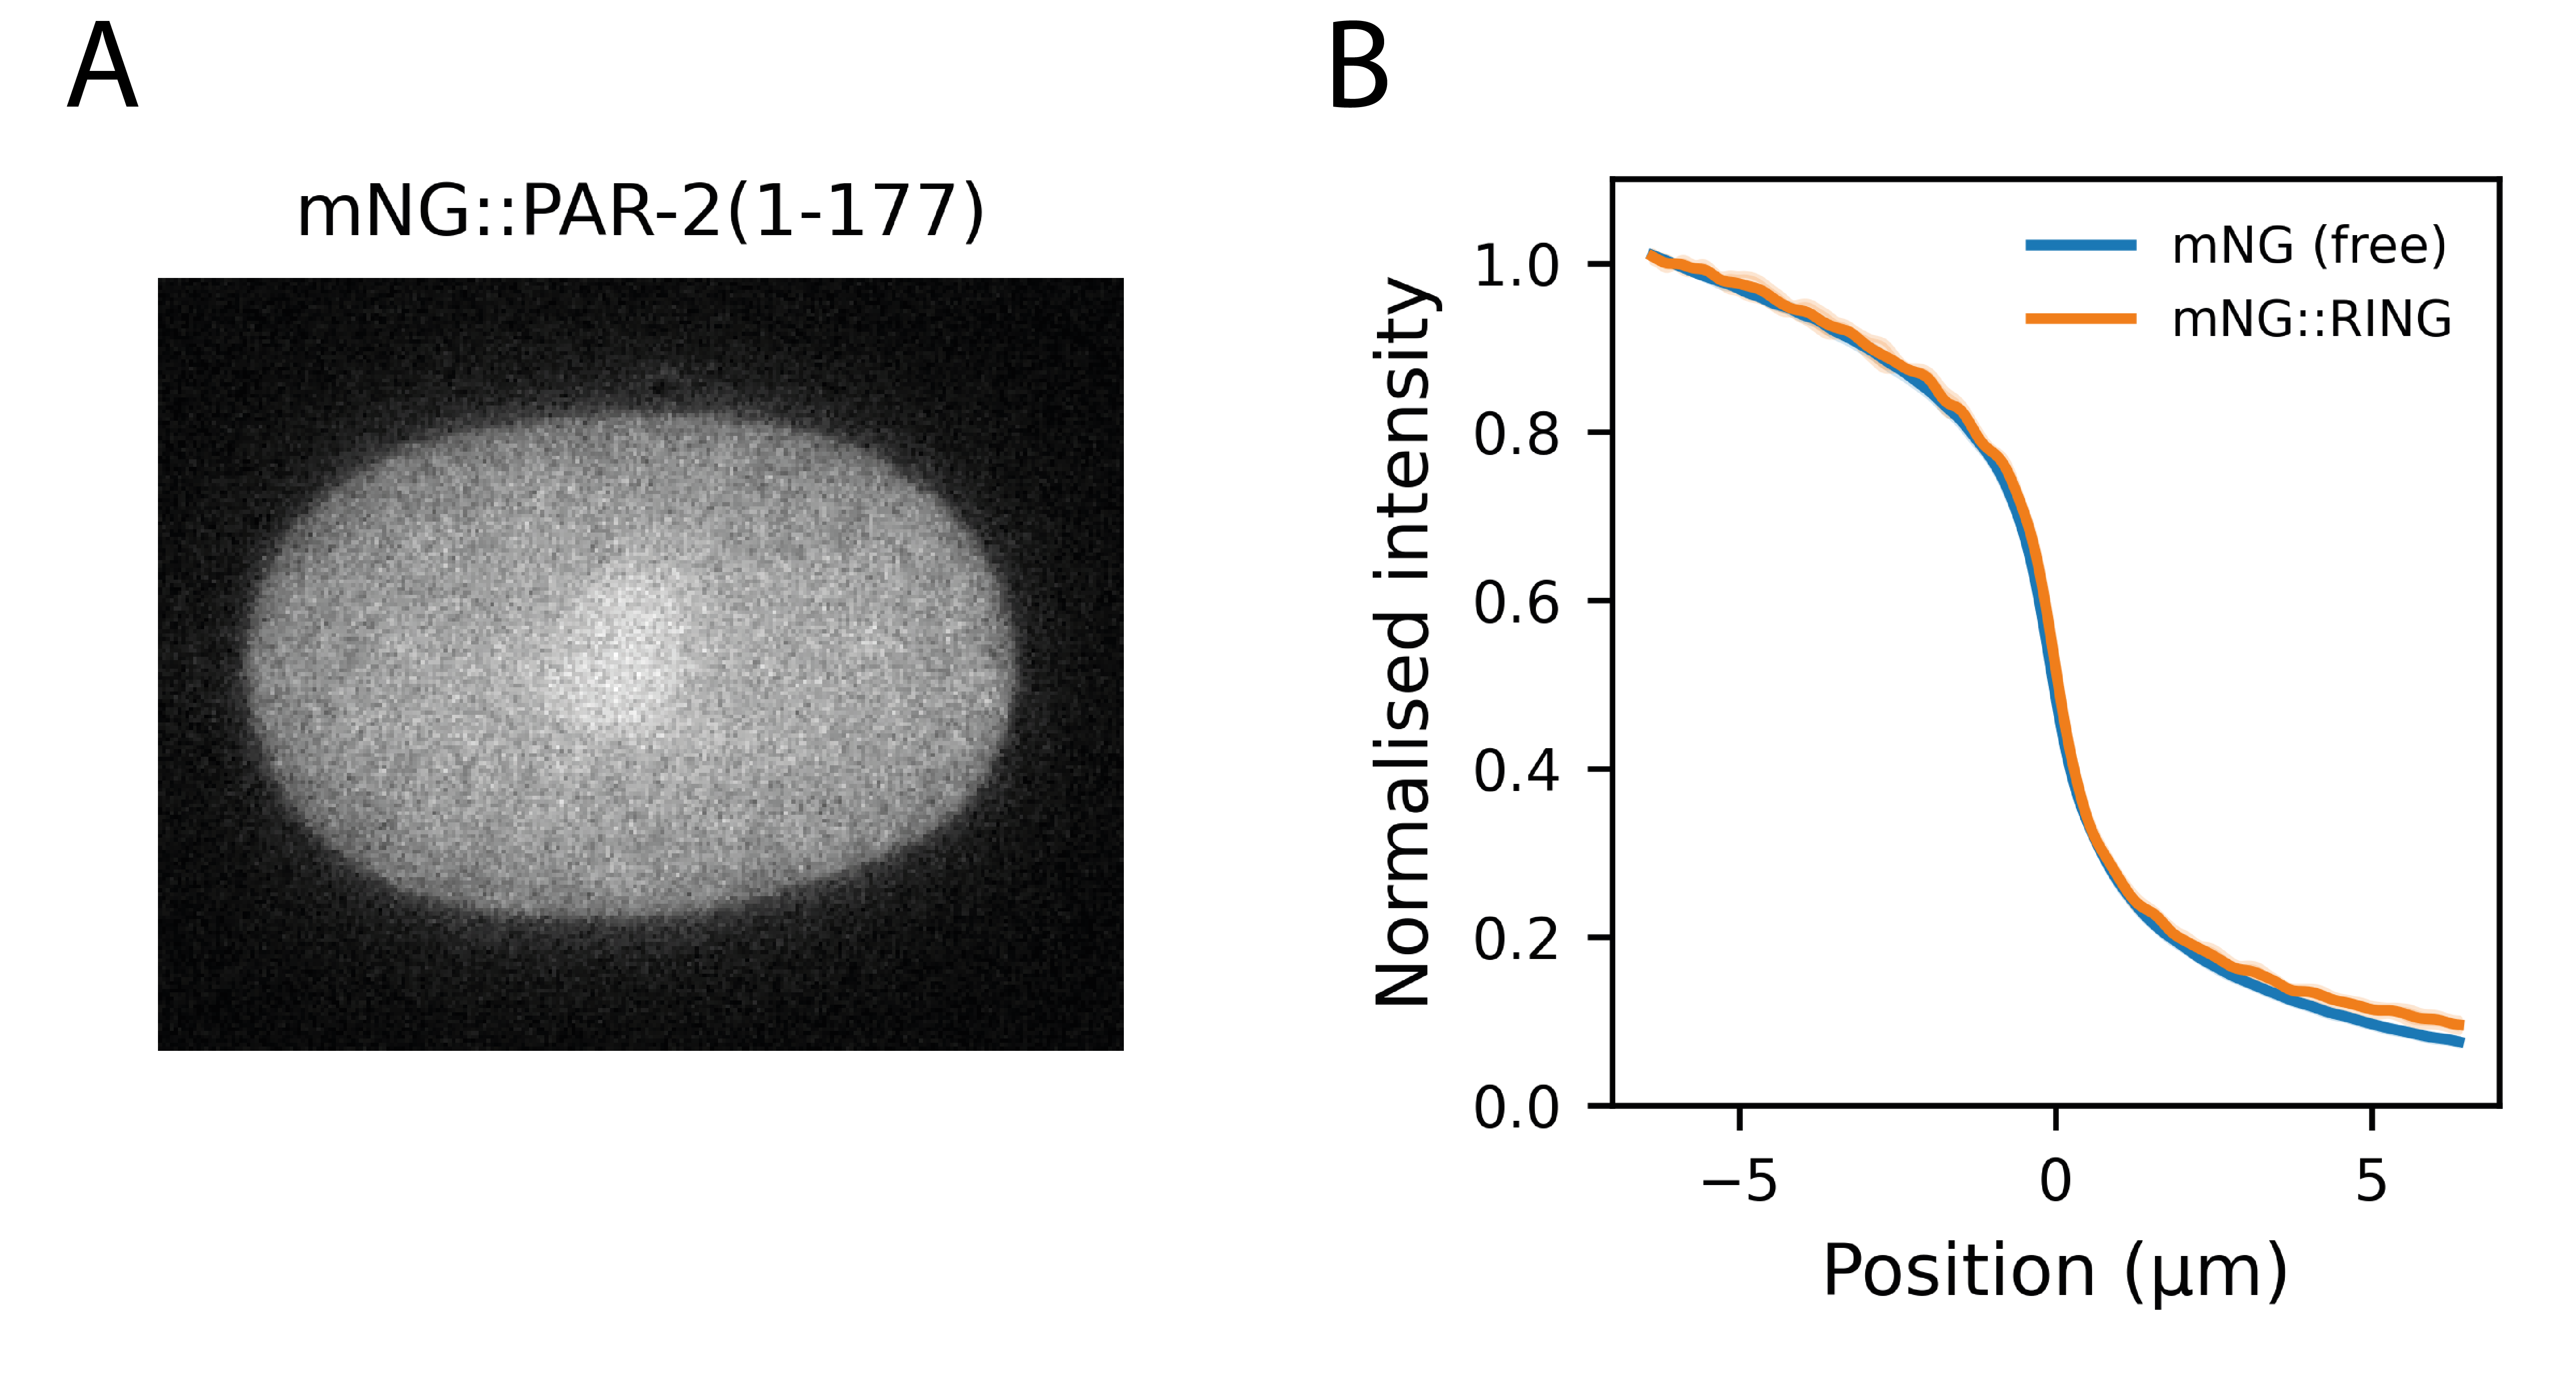
\includegraphics[scale=1]{ring_fragment_in_vivo}
\centering
\mycaption{PAR-2 RING domain fragment shows no membrane localisation}{
\textbf{(A)} Midplane image of mNG::PAR-2(1-177), showing entirely cytoplasmic localisation.
\textbf{(B)} Normalised cross-cortex profile of mNG::PAR-2(1-177) compared to mNG alone.
}
\label{fig:ring_fragment_in_vivo}
\end{figure}

To investigate this, I used a pleckstrin homology (PH) plasma membrane probe to tether the RING-containing fragment to the plasma membrane. Should this construct be capable of dimerising with endogenous PAR-2, we would expect preferential enrichment in the posterior of the cell. I found that construct was poorly expressed in zygotes, but visible after autofluorescence correction by SAIBR. Whilst PH alone is uniform on the membrane, tethering it to the PAR-2 RING domain causes clear enrichment in the posterior, which is indicative of an interaction with endogenous PAR-2 (\cref{fig:ph_ring}). A C56S mutant construct, by contrast, shows a reduced degree of polarity compared to the wild type probe (\cref{fig:ph_ring}B-D).\\

\begin{figure}[!h]
\includegraphics[scale=1]{ph_ring_v2}
\centering
\mycaption{Membrane-tethered RING domain fragment drives posterior localisation}{
\textbf{(A)} Schematic of the three constructs tested (GFP not shown).
\textbf{(B)} Midplane confocal images of the three constructs.
\textbf{(C)} Quantification of membrane to cytoplasmic ratios for the three constructs (Mean $\pm$ SD).
\textbf{(D)} i. Quantification of asymmetry index (see Methods) using the data in (C).
ii. Probability distributions of effect sizes in the data, estimated by bootstrapping. Vertical lines indicate 95\% confidence intervals.
}
\label{fig:ph_ring}
\end{figure}

These results imply that the GFP::PH::RING construct polarises by dimerising with polarised endogenous PAR-2. Following from these results, it is expected that disrupting polarity of endogenous PAR-2 should disrupt posterior bias of the membrane-tethered RING domain. To test this, I disrupted endogenous polarity using RNAi against \textit{par-2} or \textit{par-6}, and visualised the effect on the GFP::PH::RING construct. As expected, if PAR-2 is uniform (\textit{par-6} RNAi) or absent (\textit{par-2} RNAi), the membrane tethered RING domain reverts to a more uniform localisation (\cref{fig:ph_ring_rnai}).\\

\begin{figure}
\includegraphics[scale=1]{ph_ring_rnai_v2}
\centering
\mycaption{Localisation of membrane-tethered RING domain is dependent on endogenous PAR patterns}{
\textbf{(A)} Midplane confocal images of GFP::PH::RING under conditions of no RNAi, \textit{par-2} RNAi and \textit{par-6} RNAi.
\textbf{(B)} Quantification of membrane to cytoplasmic ratios for the three constructs (Mean $\pm$ SD).
\textbf{(C)} i. Quantification of asymmetry index (see Methods) using the data in (C).
ii. Probability distribution of effect sizes in the data, estimated by bootstrapping. Vertical lines indicate 95\% confidence intervals.
}
\label{fig:ph_ring_rnai}
\end{figure}


\subsection{Mutation to dimerisation interface weakens membrane association in vivo}

Overall, the data described so far suggests a mechanism whereby cytoplasmic PAR-2 is monomeric, and enrichment on the membrane switches PAR-2 to a dimeric state via a concentration-dependent dimerisation reaction. I next aimed to investigate the potential importance of this dimerisation reaction in vivo. As discussed previously, unfolding the RING domain by targeted mutation to a zinc-interacting cysteine has a strong phenotype in vivo, characterised by a strong reduction in membrane affinity. However, as C56S mutation is expected to disrupt the tertiary structure of the whole domain, rather than just the dimerisation interface, it may also have additional effects. Structure prediction analysis and SEC-MALS data indicate that a single mutation to a hydrophobic residue in the putative dimerisation interface (L109R) is sufficient to specifically disrupt dimerisation. To investigate the significance of PAR-2 dimerisation in vivo, I performed targeted mutations to this site by CRISPR in an mNG::PAR-2 background. In addition to L109R, I performed an additional L to R mutation to L50, which is found in the putative N-helix, and is not expected to interact with L109 (\cref{fig:l50_structure}).\\

\begin{SCfigure}
\includegraphics[scale=0.8]{l50_structure}
\mycaption{Position of the L50 site within the 4-helix bundle of the PAR-2 RING domain}{L50 site highlighted in blue, other residues coloured by hydrophobicity}
\label{fig:l50_structure}
\end{SCfigure}

As shown in \cref{fig:dimer_interface_mutants_in_vivo}A-C, both mutations cause a strong reduction in membrane affinity. The effect is stronger for L109R than L50R, which may suggest that L50R has a weaker disruptive effect on dimerisation. Combining both mutants has no effect compared to L109R alone (\cref{fig:dimer_interface_mutants_in_vivo}D), which implies that dimerisation is completely disrupted in L109R. Interestingly, however, neither mutant reduces membrane affinity to the same extent as C56S. Assuming that dimerisation is fully disrupted by L109R, this implies that fully unfolding the domain may have additional effects compared to just disrupting dimerisation alone. One plausible explanation is that, in the case of C56S, the unfolded domain interferes with normal membrane binding, and therefore has an additional negative effect on membrane affinity. Compatible with this, a PH::RING fusion has lower overall membrane affinity than PH alone (\cref{fig:ph_ring}). Combining C56S and L109R has no effect compared to C56S alone (\cref{fig:dimer_interface_mutants_in_vivo}E), suggesting that dimerisation is completely disrupted in the C56S mutant.\\

\begin{figure}
\includegraphics[scale=0.9]{dimer_interface_mutants_in_vivo_v2}
\centering
\mycaption{Dimerisation interface mutants disrupt PAR-2 membrane association}{
\textbf{(A)} Midplane confocal images of wild type, L50R, L109R and C56S PAR-2.
\textbf{(B)} Normalised cross-cortex profiles for the four PAR-2 alleles in (A).
\textbf{(C)} Quantification of membrane to cytoplasmic ratio for the four mutants and (A) and (B). Bottom: probability distributions of effect sizes in the dataset, estimated by bootstrapping.
\textbf{(D)} Membrane affinity quantification of double L50R+L109R mutant shows no effect compared to L109R alone. Right: probability distributions of effect sizes in the dataset, estimated by bootstrapping.
\textbf{(E)} Membrane affinity quantification of double C56S+L109R mutant shows no effect compared to C56S alone. Right: probability distributions of effect sizes in the dataset, estimated by bootstrapping. Vertical lines in C (bottom), D (right) and E (right) show 95\% confidence intervals.
}
\label{fig:dimer_interface_mutants_in_vivo}
\end{figure}

% Rundown data wt vs L109R?

\begin{comment}

\begin{figure}
\includegraphics[scale=1]{l109r_rundown}
\centering
\mycaption{PAR-2 membrane binding nonlinearity is reduced in L109R mutant}{
\textbf{(A)} Quantification of membrane and cytoplasmic concentration for wild type and L109R PAR-2 in embryos with varying PAR-2 dosage (achieved by RNAi). Untagged N2 embryos shown in white.  Solid lines indicate fit of each dataset to an exponent model ($y = ax^b$). Shaded regions show 95\% confidence intervals, estimated by bootstrapping.
\textbf{(B)} Probability distributions of exponents from model fitting in (A), estimated by bootstrapping. Vertical lines indicate 95\% confidence intervals.
}
\label{fig:l109r_rundown}
\end{figure}

\end{comment}

To determine the effects of these mutants on organism development, I investigated levels of embryonic lethality and adult sterility. PAR-2 null mutants typically display embryonic lethality, as zygotic polarity is disrupted. Sterility is a common phenotype associated with partially penetrant PAR-2 defects, as PAR-2 is important in stabilising germ line identity in the P lineage. Data for my mutants (\cref{fig:ring_lines_lethality_sterility}) shows that, whilst lines harboring a C56S mutation have high levels of lethality and sterility, this is not the case for the dimerisation interface mutants. It may be that the additional loss of membrane affinity in C56S mutants has a significant impact on pPAR domain integrity, which may be important in later developmental stages as well as in the zygote. Even though no effects were observed for L50R and L109R compared to wild type, it is likely that defects would be observed in non wild-type backgrounds (e.g. LGL-1 mutant), or with reduced PAR-2 expression (e.g. heterozygous). This remains to be investigated.\\

\begin{figure}
\includegraphics[scale=1]{ring_lines_lethality_sterility}
\centering
\mycaption{Embryonic lethality and adult sterility in RING mutant lines}{
\textbf{(A)} Percentage embryonic lethality. Individual points represent the percentage of dead embryos laid by one gravid adult worm over a period of 5 hours at room temperature.
\textbf{(B)} Percentage adult sterility. Individual points represent the percentage of sterile worms in the total progeny of one adult worm 48 hours after egg laying.
}
\label{fig:ring_lines_lethality_sterility}
\end{figure}


\subsection{Discussion}

With this data, I hope that I have made a convincing case that the RING domain of PAR-2 can act as a dimerisation domain. My assays show that, in vivo, dimerisation of PAR-2 appears to be restricted to the membrane. A simple explanation for this could be that effective concentrations are much higher on the membrane than in the cytoplasm, and so membrane-enrichment could be responsible for driving concentration-dependent dimerisation. I cannot rule out that the membrane-interaction strengthens dimerisation through other means, perhaps by altering folding of the protein. However, given that the RING domain fragment can clearly dimerise in vitro without a membrane, this seems surplus to requirement.\\

It is unclear how these results relate to results described in \textcite{Arata2016}, in which the authors claim to see membrane-bound oligomers as large as tetramers. Whilst I cannot rule out the formation of larger complexes on the membrane, I have shown that the oligomeric state of the PAR-2 RING domain in vitro is a monomer-dimer mix, which is in line with the expected structure of the domain. Tetrameric RING domains do exist (e.g. PML/TRIM19 \citep{Wang2018}), but this does not appear to be the case for the PAR-2 RING. There are no other regions of PAR-2 that are known to self-associate, so it is unclear how tetramers might come about. The only other structured domain in the protein is a C-terminal ATP binding domain, removal of which has been shown to have no phenotype in vivo \citep{Hao2006}. Phase separation mediated by disordered regions of the protein might be possible \citep{Uversky2019}, as has been proposed for PAR-3 \citep{Liu2020}, although this might be expected to yield particles larger than tetramers, which the authors did not observe. It is also possible that larger complexes could be mediated by interactions with another protein, such as PAR-1. The region of PAR-2 that mediates an interaction with PAR-1 is unknown. The authors did not look at RING domain mutants, so it is unclear whether the phenomena that they observe are RING-dependent or due to another cause.\\

It is also possible that their interpretations might be an artefact of their analysis methods. Crucially, several key results in their study lie in stark contrast to other studies. Their measurements of PAR-2 membrane lifetimes are significantly lower than is generally regarded by other studies \citep{Goehring2011, Hubatsch2019a, Motegi2011}. This may account for the shape of the PAR-2 domain interface predicted by their partial differential equation (PDE) models, which is significantly sharper that in vivo observations \citep{Goehring2011, Hubatsch2019a}. Their estimates of absolute PAR-2 concentrations are also significantly higher than other studies \citep{Gross2018, Goehring2011a}. Finally, their analysis of PAR-3 is concerning. PAR-3 is generally regarded to be highly clustered on the membrane \citep{Dickinson2017}, but their particle size distributions suggest that PAR-3 clusters are smaller than the supposedly tetrameric PAR-2, which is completely counter to expectations.\\

Regardless, RING-dependent dimerisation of PAR-2 appears to be important for driving strong membrane association, as I have shown that specifically disrupting dimerisation leads to a strong reduction in membrane affinity. There may be a number of possible explanations for this. Whilst I do not see any evidence for autoubiquitination, I cannot rule this out with my data. Given that the role of RING dimerisation is so fundamentally linked to ubiquitination activity in many RING E3s, one could imagine that, if this were occurring in the case of PAR-2, then this would also be disrupted by dimer interface mutants. I cannot rule out a model like this, but in the next chapter I provide a far simpler explanation based on dimerisation alone.\\


%%%%%%%%%%%%%%%%%%%%%%%%%%%%%%%%%%%%%%%%%%%%%%%%%%%%%%%%%%
\clearpage
\chapter{Modelling the interplay between dimerisation and membrane association}

\textbf{Detailed contributions:}\\
The thermodynamic model described in section \ref{section:thermodynamic_full_model} was developed by David Zwicker at the Max Planck Institute for Dynamics and Self-Organisation in G{\"o}ttingen, Germany. All the analysis presented in this chapter was performed by myself.\\

\clearpage
\section*{Notation}

I will use the following symbols throughout the chapter to describe to the chemical properties of an equilibrium system:\\

\begin{tabular}{ll}
$G$ & total Gibbs energy of the system\\
$G_x$ & Gibbs energy of a system of pure $x$\\
$n_x$ & number of moles of $x$\\
$\mu_x$ & chemical potential of $x$\\
$\mu_x^{\circ}$ & standard chemical potential of $x$\\
$c_x$ & molar concentration of $x$\\
$c^{\circ}$ & the standard concentration\\
$R$ & the gas constant\\
$T$ & temperature in kelvins
\end{tabular}


\clearpage
\section{Introduction}

In the previous chapter, I showed that the RING domain of PAR-2 can dimerise, and that membrane bound PAR-2 is, at least partially, dimeric. I also showed that a series of RING domain mutants have a lower membrane affinity, suggesting that dimerisation may be fundamental for achieving high membrane affinity. Added to this, I have shown that wild type PAR-2 displays nonlinear membrane association, which is disrupted in RING domain mutants. This suggests that dimerisation may lead to a form of positive feedback, whereby membrane affinity is enhanced as protein concentrations increase.\\

In this chapter, I investigate the potential link between these characteristics, and, more generally, investigate the extent to which dimerisation can influence the membrane binding behaviour of a protein. To do so, I will use chemical thermodynamics to model dimerisation and membrane binding in an equilibrium system. I will begin this chapter by introducing the general modelling framework, and will then use this framework to describe a model which incorporates dimerisation and membrane association. I will then use this model to investigate the potential influence of dimerisation on membrane association, and compare this to in vivo data of PAR-2 membrane association. Specifically, I investigate the extent to which the nonlinearity of PAR-2 membrane association can be accounted for by protein dimerisation, and whether differences in the membrane association behaviour of wild type PAR-2 and RING domain mutants can be accounted for by disruption to dimerisation.\\

% Thermodynamic equilibrium puts constraints on the behaviour of a system, and allows us to accurately describe behaviour with a small number of easily interpretable parameters. 


\clearpage
\section{Modelling chemical equilibria}
\label{sec:modelling_chemical_equilibria}

In a chemical reaction, chemical equilibrium is a state in which reactants and products are present at concentrations that have no tendency to change over time. Consider a closed system in which material is exchanging between two states, \textbf{a} and \textbf{b}:
\begin{center}
\ce{\textbf{a} <=> \textbf{b}}
\end{center}

Provided there are no additional inputs, the system will eventually reach an equilibrium in which the rates of the forward and reverse reactions are equal, and concentrations have no tendency to change over time. Energetically speaking, this equilibrium is reached when the total Gibbs free energy of the system ($G$) is minimised. This minimum energy at equilibrium ($G_{min}$) will be lower than the energy of a system of either pure \textbf{a} ($G_a$) or pure \textbf{b} ($G_b$), and so, regardless of how the system is initiated, the system will eventually stabilise with a mixture of the two states (\cref{fig:gibbs_profile}).\\ 

\begin{SCfigure}
\includegraphics[scale=0.9]{gibbs_profile}
\mycaption{Gibbs energy profile for a system at equilibrium}{
Plot of the Gibbs energy of a system as a function of composition for a species converting between states \textbf{a} and \textbf{b} (where a composition of 0 means entirely in state \textbf{a} and 1 means entirely in state \textbf{b}). $G_a$ and $G_b$ represent the Gibbs energy of the system when all molecules are in state \textbf{a} or state \textbf{b}. The system reaches an equilibrium when $G$ is minimised ($G_{min}$), at which point the equilibrium concentration of \textbf{b} is $b_{eq}$ and \textbf{a} is (1 - $b_{eq}$).
}
\label{fig:gibbs_profile}
\end{SCfigure}

The position of equilibrium will depend on the intrinsic energetics of the two species. For example if $G_a$ is lower than $G_b$ (meaning that pure \textbf{a} is more energetically favourable than pure \textbf{b}), as is shown in \cref{fig:gibbs_profile}, the system will stabilise in a state with more \textbf{a} than \textbf{b}. Formally, we can describe $G$ according to the molar amounts of \textbf{a} and \textbf{b} ($n_a$ and $n_b$), and their associated chemical potentials ($\mu_a$ and $\mu_b$):
\begin{equation}
G = n_a \mu_a + n_b \mu_b
\label{eq:gibbs}
\end{equation}

Chemical potentials describe the Gibbs free energy density of each component in a mixture (i.e. energy per mole). These values vary with the molar concentration of each species ($c_a$ and $c_b$), and using ideal solution theory can be described as:
\begin{align}
\mu_a &= \mu_a^{\circ} + RT \ln \frac{c_a}{c^{\circ}}\\
\mu_b &= \mu_b^{\circ} + RT \ln \frac{c_b}{c^{\circ}}
\end{align} 

where $c^{\circ}$ is the standard concentration (usually defined as 1 mol dm$^{-3}$) and $\mu_a^{\circ}$ and $\mu_b^{\circ}$ are the standard chemical potentials of \textbf{a} and \textbf{b} (i.e. chemical potentials at the standard concentration). $R$ and $T$ are the gas constant and temperature in kelvins, respectively. For a 1 litre system containing 1 mole of \textbf{a} or \textbf{b}, $\mu_a^{\circ}$ and $\mu_b^{\circ}$ are equivalent to $G_a$ and $G_b$ in \cref{fig:gibbs_profile}.\\

Equilibrium concentrations of \textbf{a} and \textbf{b} can be found by finding the point at which \cref{eq:gibbs} is minimised (i.e the point at which the derivative of $G$ ($dG$) as a function of system composition is zero). By considering how $G$ changes when a small amount ($dn$) of \textbf{a} is converted to \textbf{b}:
\begin{equation}
dG = - dn \mu_a + dn \mu_b
\end{equation}

we can see $dG$ approaches zero when $\mu_a = \mu_b$. Therefore, equilibrium concentrations of \textbf{a} and \textbf{b} can be found by solving the equilibrium condition:
\begin{equation}
\mu_a = \mu_b
\label{eq:equilibrium_condition_simple}
\end{equation}

Since the total amount of material is conserved, we can impose the initial constraint that:
\begin{equation}
c_{tot} = c_a + c_b
\label{eq:mass_conservation_simple}
\end{equation}
where $c_{tot}$ is a constant representing the total concentration of material. Solving equations \ref{eq:equilibrium_condition_simple} and \ref{eq:mass_conservation_simple}, equilibrium concentrations of \textbf{a} and \textbf{b} can be expressed as:
\begin{align}
c_a &= \frac{c_{tot}}{1 + e^{(\mu_a^{\circ} - \mu_b^{\circ})/RT}}\\
c_b &= \frac{c_{tot}}{1 + e^{(\mu_b^{\circ} - \mu_a^{\circ})/RT}}
\end{align}

Additionally, the following relationship always holds true:
\begin{equation}
\frac{c_a}{c_b} = e^{(\mu_b^{\circ} - \mu_a^{\circ})/RT}
\end{equation}

showing that, regardless of the total amount of material, there is a constant ratio between the two states at equilibrium. The ratio that is reached will depend on the standard chemical potentials of each state. When $\mu_a^{\circ} < \mu_b^{\circ}$ the system will stabilise with more \textbf{a} than \textbf{b}, and vice versa (\cref{fig:thermodynamic_simple_example2}).\\

\begin{figure}
\includegraphics[scale=0.9]{thermodynamic_simple_example2}
\centering
\mycaption{Schematic of thermodynamic equilibrium for a substance exchanging between two states}{
As shown, the position of equilibrium depends on the standard chemical potentials of each state ($\mu_a^{\circ}$ and $\mu_b^{\circ}$).}
\label{fig:thermodynamic_simple_example2}
\end{figure}

We can apply a similar description to a species that is exchanging between two physical compartments. In this case \textbf{a} and \textbf{b} can represent material in two spatial compartments, with $\mu_a^{\circ}$ and $\mu_b^{\circ}$ representing the standard chemical potentials associated with each compartment. The chemical potential equations take on the same form as above, although we can make the following adjustment to the conservation of mass term to account for potential differences in the volume of the two compartments:
\begin{equation}
c_{tot} = c_a + \alpha c_b
\end{equation}

where $\alpha$ is a dimensionless factor comparing the volume of the two compartments. (In this case $c_{tot}$ can be interpreted as the concentration in compartment \textbf{a} when all molecules are in compartment \textbf{a}). As before, chemical equilibrium implies a linear relationship between concentrations in the two compartments, and the concentration ratio between compartments is specified by $\mu_b^{\circ} - \mu_a^{\circ}$ (\cref{fig:thermodynamic_simple_example}).\\

\begin{figure}
\includegraphics[scale=0.9]{thermodynamic_simple_example}
\centering
\mycaption{Schematic of thermodynamic equilibrium for a substance exchanging between two compartments}{
As shown, the position of equilibrium depends on the standard chemical potentials of the substance associated with each compartment ($\mu_a^{\circ}$ and $\mu_b^{\circ}$). In this example, the volume ratio between the compartments ($\alpha$) is equal to 1.}
\label{fig:thermodynamic_simple_example}
\end{figure}



\clearpage
\section{A thermodynamic model of dimerisation and membrane association}
\label{section:thermodynamic_full_model}

Now that I have introduced the modelling framework, we can begin to use this approach to understand the equilibrium behaviour of PAR-2 in a cellular environment. Specifically, I aim to model dimerisation of PAR-2, and its interaction with the plasma membrane, to understand how these behaviours might interact with each other. I will begin by building individual thermodynamic descriptions of membrane association and dimerisation, before describing a full model which combines both features.\\

\subsection{Thermodynamic description of membrane association}
\label{section:thermodynamic_membrane_binding}

PAR-2 binds to the inner surface of the plasma membrane via electrostatic charge, and undergoes a continuous exchange between membrane bound (\textbf{m}) and cytoplasmic (\textbf{c}) states:

\begin{center}
\ce{c <=> m}
\end{center}

At equilibrium, the forward and reverse reactions occur at equal rates, and concentrations have no tendency to change over time. For now, we can consider the \textit{par-3 (it71)} condition discussed in chapter 3, in which PAR-2 is not being phosphorylated by PKC-3 and is uniformly distributed on the plasma membrane without diffusive fluxes, to be close to equilibrium. (In chapter 7 I will return to this point, and discuss conditions in which this may not be the case). \\

In the previous section I described an approach to model the equilibrium behaviour of a particle exchanging between two spatial compartments. We can use a similar description for a protein exchanging between membrane-bound and cytoplasmic states, by considering membrane and cytoplasm as two volume compartments. In this case the membrane compartment can be described as a thin volume between the plasma membrane and the cytoplasm (\cref{fig:thermodynamic_membrane_binding_schematic}). In this very simple description, if we assume that motion of membrane-bound molecules is confined to two dimensions along the inner surface of the plasma membrane, the effective thickness of the membrane compartment will be equal to the diameter of the protein ($D$). Therefore, the volume ratio between the two compartments can be given as $D\psi$, where $\psi$ is the surface area to volume ratio, and the total amount of protein can be described as:
\begin{equation}
c_{tot} = c_c + D\psi c_m
\end{equation}

where $c_m$ and $c_c$ are molar concentrations in the cytoplasmic and membrane compartments, and $c_{tot}$ is the total amount of protein (i.e. the cytoplasmic concentration when all molecules are cytoplasmic).\\

\begin{SCfigure}
\includegraphics[scale=1]{thermodynamic_membrane_binding_schematic}
\mycaption{Schematic of equilibrium model for membrane association}{
The system can be described as two volume compartments representing cytoplasmic and membrane-bound states. We assume that diffusion in the membrane compartment is confined to the two-dimensional plane of the plasma membrane, so the membrane compartment can be described as a volume with thickness $D$, where $D$ is equal to the diameter of the molecule.
}
\label{fig:thermodynamic_membrane_binding_schematic}
\end{SCfigure}

We can see from the analysis in the previous section that equilibrium concentrations depend only on the difference between $\mu^{\circ}$ terms. Therefore, for the purpose of determining equilibria, we can define chemical potentials as:
\begin{align}
\mu_c &= RT \ln \frac{c_c}{c^{\circ}}\\
\mu_m &= RT \ln \frac{c_m}{c^{\circ}} - w_m
\end{align} 

where $w_m$ represents the energetic difference between the cytoplasmic and membrane states (i.e. $\mu_c^{\circ} - \mu_m^{\circ}$). Therefore, similar to the description in section \ref{sec:modelling_chemical_equilibria}, membrane to cytoplasmic ratios at equilibrium are expected to be constant, according to the value of $w_m$:
\begin{equation}
\frac{c_m}{c_c} = e^{w_m/RT}
\end{equation}


\subsection{Thermodynamic description of dimerisation}
\label{section:thermodynamic_dimerisation}

We can use similar analysis to consider a dimerisation reaction:

\begin{center}
\ce{2x_1 <=> x_2}
\end{center}

where x$_1$ represents a monomer and x$_2$ represents a dimer. Chemical potentials can be described as:
\begin{align}
\mu_{x_1} &= RT\ln \frac{c_{x_1}}{c^{\circ}} \\
\mu_{x_2} &= RT\ln  \frac{c_{x_2}}{c^{\circ}} - w_d
\end{align} 

where $w_d$ represents the dimerisation energy (i.e. the energetic difference between the monomeric and dimeric states ($\mu_{x1}^{\circ} - \mu_{x2}^{\circ}$)). Thermodynamic equilibrium is reached when $2\mu_{x_1} = \mu_{x_2}$ (the factor of 2 accounting for the differing stoichiometry between the two species), leading to the following relationship:
\begin{equation}
\frac{c_{x_2}\:c^{\circ}}{(c_{x_1})^2} = e^{w_d/RT}
\end{equation}

Therefore, concentrations of dimeric protein will vary with the square of monomer concentrations (\cref{fig:thermodynamic_simple_dimer}A). With the constraint that $c_{tot} = c_{x1} + c_{x2}$, we can derive relationships for the concentrations of monomer and dimer as a function of total protein:
\begin{align}
c_{x_1} &= \frac{1}{2}e^{-w_d/RT}\left(\sqrt{4e^{w_d/RT} \frac{c_{tot}}{c^{\circ}} + 1} - 1\right)c^{\circ}\\
c_{x_2} &= c_{tot} - \frac{1}{2}e^{-w_d/RT}\left(\sqrt{4e^{w_d/RT} \frac{c_{tot}}{c^{\circ}} + 1} - 1\right)c^{\circ}
\end{align}

Plotting these functions, we can see that the total fraction of protein in the dimeric state is expected to increase as a function of protein amounts (\cref{fig:thermodynamic_simple_dimer}B). Note that in this description, $c_{x_2}$ is related not to the number of dimer molecules but the number of protein monomers in the dimeric state.\\

\begin{figure}
\includegraphics[scale=1]{thermodynamic_simple_dimer}
\centering
\mycaption{Dimerisation reactions lead to nonlinear equilibrium behaviour}{
\textbf{(A)} At equilibrium, dimer concentrations vary with the square of monomer concentrations.
\textbf{(B)} The total fraction of protein in the dimeric state increases as the concentration of total material increases. Parameters used: $c^{\circ} = 1$ M, $w_d / RT = 10$. Concentrations in molar units.}
\label{fig:thermodynamic_simple_dimer}
\end{figure}


\subsection{Combining membrane association and dimerisation}

So far, I have explored how dimerisation and membrane binding reactions can be described in simple thermodynamic terms. In this section I combine these descriptions to explore the potential interplay between dimerisation and membrane binding.\\

In a system in which a protein is both dimerising and exchanging between membrane and cytoplasmic pools, there are four potential species to consider: membrane monomers (\textbf{m$_1$}), membrane dimers (\textbf{m$_2$}), cytoplasmic monomers (\textbf{c$_1$}) and cytoplasmic dimers (\textbf{c$_2$}) (\cref{fig:thermodynamic_model_species}A). We can describe chemical potentials for these four species as:
\begin{align}
\mu_{c_1} &= RT\ln(c_{c_1} / c^{\circ})\\
\mu_{c_2} &= RT\ln(c_{c_2} / c^{\circ}) - w_d\\
\mu_{m_1} &= RT\ln(c_{m_1} / c^{\circ}) - w_m\\
\mu_{m_2} &= RT\ln(c_{m_2} / c^{\circ}) - 2w_m - w_d
\end{align}

where $w_m$ is the membrane binding energy and $w_d$ is the dimerisation energy. Here, we make the simple assumptions that a molecule in a dimer has twice the membrane binding energy of monomer (as dimers have membrane binding interfaces from each of two monomers), and that the dimerisation energy is equal in the membrane and cytoplasm. Chemical equilibrium is then reached when:
\begin{equation}
2\mu_{c_1} = \mu_{c_2} = 2\mu_{m_1} = \mu_{m_2}
\label{eq:four_species_equilibrium}
\end{equation}

Since the total amount of material is conserved, we have the initial constraint that:
\begin{align}
c_{tot} &= c_c + D \psi c_m
\label{eq:four_species_mass_conservation}
\end{align}

where $c_c = c_{c_1} + c_{c_2}$ and $c_m = c_{m_1} + c_{m_2}$, $D$ is the protein diameter, and $\psi$ is the surface area to volume ratio. For a given amount of total protein, equations \ref{eq:four_species_equilibrium} and \ref{eq:four_species_mass_conservation} can be solved to calculate equilibrium concentrations of each of the four species.\\

I first investigated how the equilibrium state of a system with a fixed total amount of protein ($c_{tot}$), varies depending on the two energy parameters: $w_m$ and $w_d$ (\cref{fig:thermodynamic_model_species}B). This analysis reveals that there are energy regimes in which each of the four states are favoured. With low $w_d$ and low $w_m$ protein will largely by cytoplasmic and monomeric; with low $w_d$ and high $w_m$ protein will be largely membrane-bound and monomeric; with high $w_d$ and low $w_m$ protein will be largely cytoplasmic and dimeric; and with high $w_d$ and high $w_m$ protein will be largely membrane-bound and dimeric. At intermediate energies a mix of states can be observed.\\

\begin{figure}
\includegraphics[scale=0.9]{thermodynamic_model_species}
\centering
\mycaption{The equilibrium state of a four-species dimerisation model varies depending on the interaction energies}{
\textbf{(A)} Schematic of the four species in the system.
\textbf{(B)} The equilibrium state as a function of the membrane association energy ($w_m$) and dimerisation energy ($w_d$). Shows the total amount of protein in each of the four states as a fraction of total protein. $c_{tot} / c^{\circ} = 10^{-5}$, $D\psi$ = 0.001}
\label{fig:thermodynamic_model_species}
\end{figure}

We can also see that the total amount of protein bound to the membrane ($m_1$ + $m_2$) varies according to both $w_m$ and $w_d$. By stabilising the high affinity dimeric state, increases to $w_d$ can increase overall membrane localisation for a constant $w_m$\\


\subsection{Intermediate dimerisation can drive nonlinear membrane association}

I next investigated how the system responds to varying total protein amounts. As previously described, the equilibrium state of dimerisation reactions varies as a function of total concentration, with more concentrated systems favouring increased dimerisation (\cref{fig:thermodynamic_simple_dimer}B). We would therefore expect that, in a model involving both dimerisation and membrane association, the equilibrium state should vary depending on total protein amounts.\\

In the absence of dimerisation, membrane and cytoplasmic concentrations have a defined ratio (section \ref{section:thermodynamic_membrane_binding}), and therefore will vary linearly as protein amounts are changed. In a system in which protein can dimerise, this is no longer the case. Figure \ref{fig:thermodynamic_model_feedback} shows that, in certain parameter regimes, a nonlinear relationship can be observed between cytoplasmic and membrane concentrations, with an effective exponent varying between 1 (linear relationship) and 2 (quadratic relationship).\\

\begin{figure}
\includegraphics[scale=1]{thermodynamic_model_feedback}
\centering
\mycaption{Intermediate dimerisation can drive nonlinear membrane association}{
\textbf{(A)} The relationship between cytoplasmic and membrane concentrations at equilibrium, found by modelling systems with varying amounts of total protein (ranging from $c_{tot} = 10^{-7}$ to $c_{tot} = 10^{-5}$). Curves are colour coded according to the value of $w_d$, corresponding to the coloured points in (B).
\textbf{(B)} The effective exponent of the membrane versus cytoplasm relationship across parameter space. Exponents were calculated by fitting curves such as those shown in (A) to the equation $c_m/c^{\circ} = \alpha \: (c_c/c^{\circ})^{\beta}$, with $\beta$ taken as the effective exponent. $D\phi$ = 0.001.
}
\label{fig:thermodynamic_model_feedback}
\end{figure}

Peak nonlinearity occurs in regions with high membrane energy and intermediate dimerisation energy. This corresponds to regions of parameter space in which membrane protein is largely dimeric but cytoplasmic protein largely monomeric, across the relevant range of total protein amounts (\cref{fig:thermodynamic_model_dimer_fractions}). When $w_d$ is low, protein is unable to dimerise, even at enriched membrane concentrations, and so the system follows simple linear behaviour like the monomer system described in section \ref{section:thermodynamic_membrane_binding}. If, on the other hand, $w_d$ is too high, protein is fully dimeric in both the membrane and cytoplasm, and so the system will behave similarly to the monomeric system (albeit with a higher membrane affinity). If, on the other hand, $w_d$ is intermediate, then an asymmetry can be observed whereby protein is dimeric on the membrane but not in the cytoplasm, provided that $w_m$ is sufficiently large to set up a substantial concentration difference between the two compartments.\\

\begin{figure}
\includegraphics[scale=0.9]{thermodynamic_model_dimer_fractions}
\centering
\mycaption{The dimeric state of cytoplasmic and membrane protein as a function of $w_m$, $w_d$ and $c_{tot}$}{
Figure shows the fraction of total membrane protein (A) and total cytoplasmic protein (B) that is dimeric in models with varying $w_m$, $w_d$ and $c_{tot}$. Comparing this with \cref{fig:thermodynamic_model_feedback}, we can see that regions of peak nonlinearity occur when membrane protein is dimeric but cytoplasmic protein is monomeric.
}
\label{fig:thermodynamic_model_dimer_fractions}
\end{figure}

To understand why this leads to a nonlinear membrane binding relationship, consider an extreme case in which all cytoplasmic protein is monomeric and all membrane protein is dimeric (with the other two states being transient intermediates). In other words, we have the following equilibrium:

\begin{center}
\ce{2c_1 <=> m_2}
\end{center}

Solving for $2\mu_{c1} = \mu_{m2}$ at equilibrium, we obtain the following relationship:
\begin{equation}
\frac{c_{m2}}{c^{\circ}} = e^{2w_m + w_d} \left(\frac{c_{c1}}{c^{\circ}}\right)^2
\end{equation}

implying a quadratic relationship between cytoplasmic and membrane concentrations (i.e. membrane concentrations increase with the square of cytoplasmic concentrations).\\

Overall, this analysis shows that dimerisation can have a strong influence on the membrane binding behaviour of a protein. With the simple assumption that the membrane binding energy of a dimer is twice that of a monomer, dimerisation is expected to strongly enhance membrane affinity and overall membrane localisation. I have also shown that nonlinear membrane association behaviour can arise if dimerisation and membrane binding energies are sufficient such that dimerisation is supported on the membrane but not in the cytoplasm.\\

\clearpage
\section{Quantitative assessment of PAR-2 membrane association behaviour}

Several features of this model are particularly relevant for PAR-2. Firstly, the model suggests that a reduction in dimerisation energy ($w_d$), as would be expected for a RING-disrupting mutant, can substantially decrease membrane association, independently of the membrane association energy ($w_m$). Secondly, the model suggests that, in some parameter regimes, a nonlinear relationship can occur between cytoplasmic and membrane concentrations. This latter point has the condition that dimerisation be supported in the membrane but not the cytoplasm, both of which appear to be the case for PAR-2 in vivo.\\

To assess how well the membrane-binding behaviour of wild type and RING-mutant PAR-2 can be captured by this model, I performed a quantitative comparison of the model to in vivo measurements of cytoplasmic and membrane PAR-2 concentrations. I first asked whether the different membrane-binding behaviour of wild type and RING mutant PAR-2 can be explained purely by a difference in dimerisation energies. \\

In chapter 3, I showed that wild type PAR-2 displays nonlinear membrane association, which is disrupted in a C56S RING domain mutant. In light of results described in the chapter 4, which suggest that C56S may disrupt membrane binding by more than just disrupting dimerisation, I decided to repeat the rundown experiment described in section \ref{section:par2_rundown} using the L109R mutant as a baseline instead of C56S. The results show a similar effect, whereby L109R mutant PAR-2 follows a shallower, more linear trajectory compared to wild type PAR-2 (\cref{fig:thermodynamic_wt_vs_l109r_model_fit}).\\

% Do the same fig here to show cyt vs mem relationship?


% Ultimately this parameter influences the degree to effective concentrations are enhanced upon membrane binding, which will influence the degree to which dimeric state can differ in the membrane and cytoplasmic compartments.

To assess whether the different behaviour of WT and L109R can be explained purely by a reduction in dimerisation energy, I fit the in vivo data to a model in which $w_m$ is unchanged between the two conditions but $w_d$ allowed to change. As discussed previously, the model has a parameter $D$ describing the diameter of the protein molecule. Whilst this has not been determined for PAR-2, we can expect that, with a mass of 69.95 kDa, protein diameter should be on the order of 1-10 nm \citep{Erickson2009}. To assess the full range of model behaviours I consider $D$ at both extremes.\\

I performed model fitting by orthogonal distance regression \citep{Boggs1990}, and estimated parameter uncertainty by bootstrapping (\cref{fig:thermodynamic_wt_vs_l109r_model_fit}A, C). Optimised model parameters and 95\% confidence intervals are shown in table \ref{table:thermodynamic_model_parameters}.\\

\begin{table}[]
\begin{tabular}{|l|l|l|}
\hline
 & \textbf{Model 1 (D = 10 nm)} & \textbf{Model 2 (D = 1 nm)} \\ \hline
$w_m/RT$ & 5.94 {[}5.63, 6.10{]} & 8.24 {[}7.96, 8.41{]} \\ \hline
$w_d/RT$ (WT) & 12.99 {[}12.39, 13.88{]} & 10.66 {[}10.09, 11.51{]}\\ \hline
$w_d/RT$ (L109R) & 11.16 {[}10.16, 12.46{]} & 8.84 {[}7.83, 10.11{]} \\ \hline
$w_d/RT$ difference & 1.83 {[}1.36, 2.27{]} & 1.83 {[}1.36, 2.28{]} \\ \hline
kD fold difference & 6.21 {[}3.89, 9.69{]} & 6.22 {[}3.90, 9.81{]} \\ \hline
\end{tabular}

\mycaption{Optimised model parameters}{
Given for models in which $D$ (protein diameter) = 10 nm or 1 nm. Both models show that the data is best explained by an approximately 6-fold difference in dimerisation kD between wild type and L109R PAR-2. 95\% confidence intervals shown in square brackets.
}

\label{table:thermodynamic_model_parameters}
\end{table}

Figures \ref{fig:thermodynamic_wt_vs_l109r_model_fit}B and D show that the optimised models closely capture the data, suggesting that a reduction in dimerisation energy by approximately 1.8 $RT$ is sufficient to account for the different membrane association relationships of wild type PAR-2 and PAR-2 L109R. This corresponds to a roughly 6-fold difference in the dissociation constant (kD). (Note that the dissociation constant (kD) for dimerisation is exponentially related to the dimerisation energy, so a decrease in $w_d / RT$ by $x$ corresponds to an $e^x$ fold increase in kD.) Furthermore, we can see that the optimised models predict that cytoplasmic protein is entirely monomeric across the range of relevant concentrations, whereas wild type membrane-bound protein is mostly dimeric, which matches experimental observations. Dimerisation of PAR-2 L109R is predicted to be reduced at the membrane compared to wild type PAR-2.

% Maybe have a box for model fitting procedure?

\begin{figure}
\includegraphics[scale=0.85]{thermodynamic_wt_vs_l109r_model_fit}
\centering
\mycaption{Membrane-association behaviour of wild-type and L109R PAR-2 can be explained by a reduction in dimerisation energy}{
\textbf{(A, C)} Parameter estimates for models with $D$ (protein diameter) = 10 nm (A) or 1 nm (C). Models were fit to the in vivo data in (B) and (C) by orthogonal distance regression. Parameter uncertainty was assessed by bootstrapping. Each point represents parameters obtained from fitting a model to single bootstrap sample (an orange and a blue point with a shared $w_m$ for each sample). Black dots show parameters for a model trained on the full dataset.
\textbf{(B, D)} In vivo data (points) compared to model fits (lines, shaded regions indicate 95\% confidence intervals). $c^{\circ}$ is defined as the mean cytoplasmic concentration of wild type PAR-2 at full dosage x $10^8$. Assuming a cytoplasmic concentration of roughly 10 nM \citep{Gross2018}, this corresponds to a $c^{\circ}$ of approximately 1 M. Also shown are the dimeric states of membrane and cytoplasmic protein in the models across the range of concentrations, with 95\% confidence intervals.
}
\label{fig:thermodynamic_wt_vs_l109r_model_fit}
\end{figure}



\section{Discussion}

Overall, I have shown that a simple thermodynamic model of dimerisation and membrane association, with just four species and two interaction energies, can successfully capture the nonlinear membrane association behaviour of PAR-2, and the disruptive effects of RING domain mutants. I propose that, in vivo, cytoplasmic PAR-2 concentrations are too low for the RING to dimerise, but enrichment on the membrane enhances effective concentrations, driving concentration-dependent RING dimerisation on the membrane. This reaction has two major consequences. Firstly, as dimers can utilise membrane binding interfaces from two PAR-2 molecules, dimerisation is expected to enhance overall membrane affinities. This provides an explanation for the reduction in membrane localisation seen for all RING domain mutants (chapter 4). Secondly membrane-specific dimerisation can lead to a nonlinear relationship between concentration and membrane association, which closely matches in vivo PAR-2 data. This nonlinearity can be considered a form of positive feedback in which the effective membrane affinity increases with increasing membrane concentrations. \\

Moving forward, further experiments could be devised to test this thermodynamic formulism more rigorously. For example, the model makes certain predictions about the effects of temperature, showing a decrease in membrane affinity and membrane dimerisation as temperatures rise (\cref{fig:thermodynamic_model_temperature}). Comparison of equivalent in vivo data to these predictions could give a sense of the validity of the model. Of course, care would be needed when interpreting such an experiment, as temperature interventions might have unanticipated consequences both intrinsic to PAR-2 (e.g. changes to protein folding) and extrinsic (e.g. activation of heat shock pathways).\\

Of additional interest is the effects that this mechanism might have on the overall pattern forming capabilities of the PAR network. Oligomerisation is a common feature of many polarity proteins, and has been suggested to contribute to stable bistability in mathematical models of polarity \citep{Lang2022}. In the next chapter, I consider the specific impact that PAR-2 dimerisation may have on the patterning behaviour of the PAR network.\\

\begin{SCfigure}
\includegraphics[scale=0.9]{thermodynamic_model_temperature}
\centering
\mycaption{Modelling the effects of temperature on the membrane vs. cytoplasm relationship of PAR-2}{
Black line shows the membrane vs cytoplasm relationship of the parameterised model first shown in \cref{fig:thermodynamic_wt_vs_l109r_model_fit}B. Blue and red lines show membrane vs cytoplasm relationships for equivalent models with a 5\% decrease (blue) or 5\% increase in absolute temperature (equivalent to an increase or decrease of approximately 15$^{\circ}$C from a starting temperature of 20$^{\circ}$C).\\ \\ \\
}
\label{fig:thermodynamic_model_temperature}
\end{SCfigure}

% The model makes a number of simplifications in its description of interaction energies, such as the assumption that dimerisation energy is equal in the cytoplasm and on the membrane, and that dimers have a membrane association energy twice that of a monomer. Nevertheless, a general feature of the model, shown by equation x, is that, regardless of the values of the energy terms, as long as the system can achieve dimerisation on the membrane but not in the cytoplasm, a quadratic relationship between cytoplasmic and membrane concentrations is to be expected.\\

% The question remains as to why C56S appears more disruptive than L109R. One possibility is that dimerisation isn’t completely disrupted in L109R, although if this were the case, I’d expect L109R and L50R to be additive, which they are not. Another possibility is that C56S mutation, by causing the entire domain to unfold, has an additional negative impact on membrane binding whereby the unfolded domain interferes with the association between the polybasic domain and the membrane (effectively causing a decrease in $w_m$ in addition to $w_d$).\\

%%%%%%%%%%%%%%%%%%%%%%%%%%%%%%%%%%%%%%%%%%%%%%%%%%%%%%%%%%
\clearpage
\chapter{Assessing the impacts of PAR-2 dimerisation in polarity models}

\textbf{Detailed contributions:}\\

The transition state theory description of membrane binding kinetics presented in section \ref{section:transition_state_theory} was developed by David Zwicker, following on from work described in the previous chapter. The rest of the work is my own.\\


\clearpage
\section{Introduction}

Cell polarity is generally understood as an out-of-equilibrium process in which feedback reactions regulate the conversion of proteins between slowly diffusing plasma membrane-bound states and rapidly diffusing cytoplasmic states. So far, I have shown that PAR-2 dimerises at the membrane, and used equilibrium models to show that this reaction underlies a form of positive feedback, whereby membrane affinity increases as concentrations increase. In this section, I consider the impact that this feedback reaction might have in the context of cell polarity. \\

To consider the potential implications of dimerisation-dependent membrane association behaviour in out-of-equilibrium contexts, it is no longer sufficient to consider equilibrium states, and individual rates governing membrane association and dissociation must be considered. I therefore begin this chapter by considering the impact that dimerisation might have on membrane binding and unbinding rates. Fortunately, the thermodynamic model described in the previous chapter can be easily extended to this scenario, which I describe in the first section of this chapter. I then use this description to incorporate several features of dimerisation into existing mathematical models of PAR polarity and comment on the potential implications of dimerisation in this context.\\


\clearpage
\section{Describing membrane binding dynamics with transition state theory}
\label{section:transition_state_theory}

To begin, consider the following reaction in which a protein is exchanging between cytoplasmic ($c$) and membrane-bound ($m$) states: 
\begin{center}
\ce{$c$ <=>[$k_{on}$][$k_{off}$] $m$}
\end{center}

For a given system composition, the instantaneous flux onto the membrane ($s_{on}$) can be expressed using mass action kinetics as $k_{on} c_c$, and the total flux off the membrane ($s_{off}$) can be written as $k_{off} c_m$ (where $c_c$ and $c_m$ are cytoplasmic and membrane concentrations, respectively). Using transition state theory \citep{Hanggi1990}, these fluxes can be written in terms of the chemical potentials of each state:
\begin{align}
s_{on} &= \Lambda e^{\mu_c}\\
s_{off} &= \Lambda e^{\mu_m}
\end{align}

where $\Lambda$ is a pre-factor that scales rates according to the energetics of the transition state and the kinetics of the process. Rate constants can then be described as:
\begin{align}
k_{on} &= \Lambda e^{\mu_c} / c_c \\
k_{off} &= \Lambda e^{\mu_m} / c_m
\end{align}

Using the four-species chemical potential model described in the previous chapter, we can derive the following relative on and off rates for monomers and dimers:
\begin{align}
k_{on,1} &= \Lambda_1\\
k_{on,2} &= \Lambda_2 e^{-w_d}\\
k_{off,1} &= \Lambda_1 e^{-w_m}\\
k_{off,2} &= \Lambda_2 e^{-2w_m - w_d}
\end{align}

where $w_d$ (the dimerisation energy) and $w_m$ (the membrane association energy) are expressed in $RT$ units. Whilst the kinetic pre-factors ($\Lambda_1$ and $\Lambda_1$) may differ between monomer and dimer membrane-binding reactions, and can only be determined from detailed mechanistic insights, the simplest model is to assume that the pre-factor is the same ($\Lambda_1 = \Lambda_2$). With this in mind, these equations suggest that dimerisation in the cytoplasm and on the membrane is expected to slow membrane binding and unbinding kinetics, respectively. Furthermore, since dimerisation is concentration dependent, we expect overall rates to slow as overall concentrations increase. If we make the additional assumption that dimerisation reactions in the membrane and cytoplasm are fast relative to membrane binding, we can define instantaneous monomer and dimer concentrations as a function of overall concentrations. For example, for membrane-bound protein:
\begin{align}
c_{m1} &= \frac{1}{2} e^{-w_d} \left(\sqrt{4e^{w_d} c_m + 1} - 1\right)\\
c_{m2} &= c_m - \frac{1}{2}e^{-w_d}\left(\sqrt{4e^{w_d} c_m + 1} - 1\right)
\end{align}

where concentrations are expressed in units of $c^{\circ}$ (the standard molar concentration). (Note, this is identical to the description of dimerisation in section \ref{section:thermodynamic_dimerisation}). As a result, overall chemical potentials of membrane and cytoplasmic protein ($\mu_m$ and $\mu_c$) can be described as a function of overall concentrations ($c_m$ and $c_c$):
\begin{align}
\mu_c &= \ln(c_c) - \frac{1}{2}\ln\left(1 + 2e^{w_d} c_c + \sqrt{4e^{w_d} c_c+ 1}\right)\\
\mu_m &= \ln(c_m) - \frac{1}{2}\ln\left(1 + 2e^{w_d} c_m + \sqrt{4e^{w_d} c_m + 1}\right) - w_m
\end{align}

We can then obtain concentration-dependent rate constants describing overall membrane binding and unbinding, which take dimerisation into account (I use $*$ to indicate rate constants that vary as a function of concentration):
\begin{align}
k_{on}^* &= \frac{\Lambda}{\sqrt{2 e^{w_d} c_c + \sqrt{4 e^{w_d} c_c + 1} + 1}}\\
k_{off}^* &= \frac{\Lambda e^{-w_m}}{\sqrt{2 e^{w_d} c_m + \sqrt{4 e^{w_d} c_m + 1} + 1}}
\end{align}


Throughout this chapter, I will restrict analysis to models in which cytoplasmic protein is dilute and so predominantly monomeric, which is relevant for consideration of PAR-2. In this case, $e^{w_d} c_c$ is small, and so $k_{on}$ can be approximated as a constant. At the membrane, where concentrations are higher, $k_{off}$ is expected to change as a function of $w_m$, $w_d$ and concentration (\cref{fig:thermodynamic_model_koff}).\\

% Need to check the maths a bit. Getting kon = lambda / root2 when cc is small, but should be just lambda, no?

\begin{figure}
\includegraphics[scale=1]{thermodynamic_model_koff}
\centering
\mycaption{Describing relative off rates with transition state theory}{
\textbf{(A)} $k_{off} / \Lambda$ as a function of energy parameters $w_m$ and $w_d$ for a fixed membrane concentration ($c_m = 10^{-5}$).
\textbf{(B)} $k_{off} / \Lambda$ as a function of concentration for four different values of $w_d$, corresponding to the coloured points in (A). Whereas off rates for weakly dimeric protein (blue and orange) are insensitive (or weakly sensitive) to concentration, off rates for more strongly dimeric protein (green and red) fall sharply as membrane concentrations increase.
}
\label{fig:thermodynamic_model_koff}
\end{figure}

Overall, this analysis implies that the effects of dimerisation on membrane affinity are expected to come about largely through changes in the rate of membrane dissociation, rather than the rate of membrane association. Two separate points are important to note. Firstly, by impacting the dimeric state of membrane protein, the strength of dimer association ($w_d$) can tune the total dissociation rate of membrane protein over orders of magnitude (\cref{fig:thermodynamic_model_koff}A). Secondly, positive feedback on membrane localisation results from a decrease in membrane dissociation rates as membrane concentrations rise (\cref{fig:thermodynamic_model_koff}B). In the rest of this chapter, I aim to consider these two features separately. Firstly, I consider the extent to which membrane dissociation rates impact the behaviour of the existing PAR model in the absence of dimerisation-driven positive feedback. Secondly, I build a new model that incorporates dimerisation-driven positive feedback in the pPAR subnetwork, and explore the impacts that this has on patterning behaviour.\\


\clearpage
\section{Exploring the effects of membrane lifetime in the mutual antagonism model}
\label{section:goehring_model_off_rates}

A number of self-organising models have been used to describe PAR polarity driven by mutual antagonism, which vary in their complexity \citep{Goehring2011a, Dawes2011, Sailer2015, Arata2016, Gross2018}. However, in general, the principles governing polarity in each model are the same. Specifically, antagonistic feedback reactions regulate the conversion of proteins between slowly diffusing plasma membrane-bound states and rapidly diffusing cytoplasmic pools. Nonlinearities in these feedback reactions give systems bistability, which permits the existence of stable polarised and uniform states. Mass conservation causes the cytoplasmic pool of proteins to deplete as polarity domains grow, which has a stabilising effect on the position of the domain boundary. This is a principle shared by a variety of mass-conserved polarity models, such as the `wave-pinning' model originally described for Cdc42 polarity in yeast \citep{Mori2008}.\\

The aim of this section is to discuss the impacts of membrane lifetime in models based on these principles. For this purpose, I will base my analysis on the simplest self-organising PAR model, developed by \textcite{Goehring2011a}. This model groups aPARs and pPARs into two species (referred to as $A$ and $P$), and models antagonism as single-step reactions that depend nonlinearly on the concentration of the antagonist. To further simplify analysis, I will consider a symmetric model in which identical parameters govern the anterior and posterior species, similar to the approach used by \textcite{Hubatsch2019a} and \textcite{Trong2014}. This can be described by the following partial differential equations:
\begin{align}
\frac{\partial A_m}{\partial t} &= D \frac{\partial^2 A_m}{\partial x^2} + k_{on} A_c - k_{off} A_m - k_{ant} P_m^2 A_m\\
\frac{\partial P_m}{\partial t} &= D \frac{\partial^2 P_m}{\partial x^2} + k_{on} P_c - k_{off} P_m - k_{ant} A_m^2 P_m
\end{align}

where $x$ is the position coordinate along a one-dimensional membrane of length $L$, $D$ is the diffusion coefficient at the membrane, $k_{on}$ and $k_{off}$ are the membrane binding and unbinding rates and $k_{ant}$ is the rate of antagonism. The exponents of 2 on the antagonism terms provide the system sufficient nonlinearity to permit polarisation. With the assumption that cytoplasmic diffusion is fast, and so cytoplasmic concentrations are effectively uniform, the cytoplasmic concentrations of A and P ($A_c$ and $P_c$) can be calculated based on the total amount of material ($A_{tot}$ and $P_{tot}$) according the the conservation of mass terms below:
\begin{align}
A_c &= A_{tot} - \psi \bar{A_m}\\
P_c &= P_{tot} - \psi \bar{P_m}
\end{align}

where $\bar{A_m}$ and $\bar{P_m}$ are the average membrane concentrations of A and P, $\psi$ is the surface area to volume ratio and $A/P_{tot}$ are the total amounts of material. Default values for all parameters used in this section are shown in table \ref{tab:goehring_model_default_parameters}.

{\renewcommand{\arraystretch}{1.5}
\begin{table}[]
\scriptsize
\begin{tabular}{lllllll}
$D$ & $k_{on}$ & $k_{off}$ & $k_{ant}$ & $A/P_{tot}$ & $\psi$ & $L$ \\ \hline
0.1 $\mu m^2 s^{-1}$ & 0.1 $\mu m s^{-1}$ & 0.001-0.1 $s^{-1}$ & 0.001-1 $\mu m^4 s^{-1}$ & 1 $\mu m^{-3}$ & 0.1 $\mu m^{-1}$ & 50 $\mu m$
\end{tabular}
\mycaption{Default parameter values used for symmetric PAR model}{}
\label{tab:goehring_model_default_parameters}
\end{table}
}

\subsection{Conditions for polarisation}

Firstly, I test how off rates impact the ability of models to maintain stable polarity. To do so, I initiate models from a fully polarised state, and test for their ability to maintain polarity for 10000s without continuous external cues (\cref{fig:goehring_model_kant_koff_triggering}A, left). Parameter space analysis (\cref{fig:goehring_model_kant_koff_triggering}B) reveals that, for a given $k_{ant}$, a threshold $k_{off}$ exists below which polarity can be stably maintained. Additionally, as $k_{off}$ decreases, models can maintain polarity over a wider range of $k_{ant}$ values.\\

Previous parameter space analysis of this model has revealed the existence of parameter regimes which support the existence of stable uniform states (as is the case in vivo), and others in which the uniform state is unstable \citep{Goehring2011a, Trong2014}, but the effects of $k_{off}$ were not explicitly shown. To test this, I started models from a uniform aPAR dominant state and subjected them to a small initial asymmetry. In models where the uniform state is unstable, this small perturbation is amplified and a full pattern is formed (\cref{fig:goehring_model_kant_koff_triggering}A, right). In models where the uniform state is stable, the initial asymmetry is suppressed and uniformity is maintained. This analysis reveals that, over the range of parameters explored, the stability of the uniform state is set mainly by the value of $k_{ant}$, with $k_{off}$ only impacting stability close to the edge of the polarisable region.

\begin{figure}
\includegraphics[scale=1]{goehring_model_kant_koff_triggering}
\centering
\mycaption{Off rates and antagonism rates determine the potential for polarisation}{
\textbf{(A)} Examples of induced and spontaneous polarity. Induced polarity: models are started from a polarised state, and tested for their ability to stably maintain polarity in the absence of continuous spatial cues. Spontaneous polarity: models are started from a uniform aPAR dominant steady state, and $A_m$ and $P_m$ profiles are subjected to small gradients towards their respective poles. Models in which the uniform steady state is unstable will amplify these perturbations and spontaneously polarise.
\textbf{(B)} $k_{ant}$ / $k_{off}$ parameter space. Models were simulated for 10000s, using the two procedures described above, and scored as polarised at the end of the simulation if the membrane concentration profiles of A and P cross. The white regions correspond to models that are unpolarised at the end of both simulations, the grey region correspond to models that are polarised at the end of both simulations, and the green region indicates models that can stably maintain induced polarity but do not polarise spontaneously. Simulations in (A) were performed with $k_{off} = 10^{-2.5}$ and $k_{ant} = 10^{-3}$, which exists in the grey region. Further details on simulations and parameter space analysis are described in the Methods section.
}
\label{fig:goehring_model_kant_koff_triggering}
\end{figure}


\subsection{Low off rates strengthen pattern asymmetries}

Next, I explored how off rates impact the shape of polarised membrane patterns generated by the PAR model. Across the same $k_{ant}$ / $k_{off}$ parameter space, I simulated models starting from a polarised state, and scored models based on the asymmetry of their final membrane patterns.  I used the asymmetry index (ASI) of $P_m$ as a metric, calculated as follows:
\begin{equation}
ASI = (P_{m, post} - P_{m, ant}) /  2(P_{m, post} + P_{m, ant})
\end{equation}

where $P_{m, post}$ and $P_{m, ant}$ indicate the average membrane concentrations of $P_m$ in the posterior and anterior 50\% of the system.\\

The results (\cref{fig:goehring_model_kant_koff_asi}) show a dependence of pattern asymmetry on both $k_{ant}$ and $k_{off}$. Increasing $k_{ant}$ increases rates of antagonism for a given concentration of antagonist, which promotes high asymmetry by keeping PARs out of their opposing domains. Similarly, decreasing off rates allow antagonists to reach higher concentrations within their domains, which helps amplify nonlinear antagonism. Figure \ref{fig:goehring_model_kant_koff_asi}B shows that decreasing $k_{off}$ for a given $k_{ant}$ can strongly impact on the normalised shape of polarised patterns, until a maximum degree of asymmetry is reached.\\

\begin{figure}
\includegraphics[scale=1]{goehring_model_kant_koff_asi}
\centering
\mycaption{Low off rates strengthen pattern asymmetries}{
\textbf{(A)} Dependence of pattern asymmetry on $k_{ant}$ and $k_{off}$. 
\textbf{(B)} Dependence of normalised membrane patterns on $k_{off}$, which shows that low off rates sharpen asymmetries. Simulations in (B) were performed with $k_{ant} = 0.005$.
}
\label{fig:goehring_model_kant_koff_asi}
\end{figure}

\subsection{Low off rates enhance pattern stability}

Maintenance of polarity relies on competition between aPARs and pPARs, and therefore balanced activity between the two groups is expected to be an essential requirement for polarity. That said, recent work from the Goehring lab shows that the PAR network is surprisingly robust to imbalances in protein amounts in vivo, able to maintain its functions in the face of reductions in PAR protein amounts by over 50\% (Rodrigues et al., in prep). This warrants full exploration of the robustness of models to imbalances in protein amounts.\\

To test the robustness of models to protein imbalances, I simulated models with varying levels of $P_{tot}$, and scored their ability to maintain polarity starting from a polarised state. Models with high off rates are highly sensitive to protein amounts. Small reductions in $P_{tot}$ cause the boundary position to shift towards the posterior, and larger imbalances cause polarity to completely break down (\cref{fig:goehring_model_kant_koff_dosage_imbalance}A). Models with lower off rates, however, are more stable in the face of imbalances (\cref{fig:goehring_model_kant_koff_dosage_imbalance}B). Small imbalances cause relatively minor shifts in the boundary position, and models can withstand larger imbalances before polarity breaks down. In figure \ref{fig:goehring_model_kant_koff_dosage_imbalance}B, I show the maximum reduction in $P_{tot}$ that models can withstand before polarity breaks down, across $k_{ant}$ / $k_{off}$ parameter space. This reveals that, within the range of parameters explored, tolerance to imbalance is set mainly by $k_{off}$, and $k_{ant}$ has relatively little impact.\\

\begin{figure}
\includegraphics[scale=1]{goehring_model_kant_koff_dosage_imbalance}
\centering
\mycaption{Low off rates enhance robustness to imbalanced protein amounts}{
\textbf{(A)} Models with high off rates are strongly sensitive to imbalanced protein amounts. A small reduction in the amount of P compared to A leads to a large shift in the boundary position, whereas larger reductions cause polarity to break down
\textbf{(B)} Models with low off rates have a more stable boundary and can maintain polarity with strong imbalances in protein amounts. 
\textbf{(C)} Dependence on $k_{ant}$ and $k_{off}$ of the ability of models to withstand imbalanced in protein amounts. Shading highlights the maximum amount by which $P_{tot}$ can be reduced and polarity stably maintained. Simulations in (A) and (B) were performed with $k_{ant} = 0.005$.
}
\label{fig:goehring_model_kant_koff_dosage_imbalance}
\end{figure}

Enhanced stability in models with low off rates is likely a consequence of cytoplasmic pool depletion, which `pins' domain boundaries and limits the ability of the aPAR domain to grow when $P_{tot}$ is depleted. Compatible with this, models with infinite cytoplasmic pools generally show highly unstable domain boundaries \citep{Dawes2011}.\\

\subsection{Conclusions}

Overall, the analysis in this section shows that membrane dissociation rates can have a strong impact on the patterning capabilities of the PAR model. For a start, the ability of models to form patterns requires $k_{off}$ to be sufficiently low. In addition, decreasing off rates generally gives models properties that would be considered beneficial for robust patterning systems. Low off rates permit polarity across a wider range of antagonism rates, enhance steady state asymmetries by amplifying nonlinear feedback, and stabilise boundaries to the effects of changing protein amounts. Therefore, by simply lowering membrane dissociation rates, dimerisation is expected to strongly impact patterning behaviour. \\


\clearpage
\section{Exploring the effects of dimerisation-driven feedback in polarity models}

The analysis in the previous section considers the effects of changing fixed off rates on patterning. However, as discussed previously, dimerisation can also make off rates sensitive to membrane concentrations. In this section, I aim to explore the effects of this concentration-dependent feedback on patterning. To do so, I first describe a method for separating the effects of dimerisation on feedback and basal affinity, so that feedback can be explored independently. \\

\subsection{Separating the effects of dimerisation on membrane affinity and feedback}

Firstly, I redefine $k_{off}^*$ in terms of arbitrary parameters $k_1$ and $k_2$:
\begin{equation}
k_{off}^* = \frac{k_1}{\sqrt{2 k_2 P_m + \sqrt{4 k_2 P_m + 1} + 1}}\\
\end{equation}

In order to study the effects of feedback and membrane affinity separately, I define two additional parameters, based on the equilibrium properties of models in a uniform equilibrium system (so far neglecting antagonism, which I will return to later). I define $\alpha$ as the off rate in these equilibrium conditions, and $\epsilon$ as the fraction of membrane-bound protein in the dimeric state. For specific values of $\alpha$ and $\epsilon$, the membrane concentration at equilibrium $P_{m, eq}$, can be given as:
\begin{equation}
P_{m, eq} = \frac{\alpha P_{tot}}{\alpha \psi + 1}
\end{equation}

$k_2$ can then be given as:
\begin{equation}
k_2 = \frac{\epsilon}{P_{m, eq} (\epsilon - 1)^2}
\end{equation}

And finally $k_1$ can be given as:
\begin{equation}
k_1 = \alpha \sqrt{2 k_2 P_{m, eq} + \sqrt{4 k_2 P_{m, eq} + 1 } + 1}
\end{equation}

By expressing the off rate in terms of $\alpha$ and $\epsilon$, we can separate the effects of dimerisation on basal membrane affinity and concentration-dependent feedback (\cref{fig:epsilon_vs_koff}). (Note, since the cytoplasm is considered to be entirely monomeric, I use a fixed membrane binding rate ($k_{on}$).) \\

\begin{figure}
\includegraphics[scale=1]{epsilon_vs_koff_v2}
\centering
\mycaption{Separating the effects of dimerisation on basal membrane affinity and feedback}{
Relationship between cytoplasmic and membrane concentrations in systems with varying total protein amounts for different values of $\alpha$ (which indicates the off rate at equilibrium) and $\epsilon$ (which indicates the membrane dimeric fraction at equilibrium). Dashed line indicates the range of possible membrane and cytoplasm concentrations in a uniform system with $P_{tot}  = 1$ and $\psi = 0.1$. $\alpha$ determines the membrane affinity along this conservation of mass line and $\epsilon$ determines the degree of concentration-dependent feedback. Shown for $k_{on} = 0.1$.
}
\label{fig:epsilon_vs_koff}
\end{figure}



\subsection{Modelling aPAR to pPAR antagonism}

Next, I describe a scheme for modelling antagonism from $A_m$ to $P_m$. If we initially assume that dimerisation has no effects on antagonism, so that protein in monomeric and dimeric states is equally well antagonised, the overall flux off the membrane ($s_{off}$) can be expressed using mass action kinetics as:
\begin{equation}
s_{off} = k_{off}^* P_m + k_{ant} A_m P_m
\end{equation} 

where $k_{ant}$ is independent of concentration. (Note, in contrast to the previous section, I do not include an exponent on the antagonism terms as I wish to focus on the effects of nonlinearities provided by dimerisation.)\\

However, given that their membrane association is intrinsically more stable, it is plausible to imagine that dimers might be partially resistant to the effects of antagonism compared to monomers. If monomers and dimers are antagonised differently, then the overall rate of antagonism will depend upon the dimeric state of membrane-bound protein. To account for this, I introduce parameters $k_3$ and $\beta$, where $\beta$ scales the antagonism rate of dimers compared to monomers:
\begin{equation}
s_{off} = k_{off}^* P_m + k_3 P_{m1} + k_3 (1 - \beta) P_{m2}
\end{equation}

This allows for a full range of potential behaviours. $\beta = 0$ indicates that monomers and dimers are equally well antagonised, whereas $\beta = 1$ implies that dimers are entirely resistant to antagonism. I can then define an overall concentration-dependent rate constant for antagonism ($k_{ant}^*$) as:
\begin{equation}
k_{ant}^* = \frac{k_3 (P_{m1} + (1 - \beta) P_{m2})}{P_{m}}
\end{equation} 

where $P_{m1}$ and $P_{m2}$ are a function of overall concentration. This implies that, for any value of $\beta$ greater than zero, the overall rate of antagonism will change according to the dimeric state of $P_m$. To control the rate of antagonism independently of dimerisation, I introduce parameter $\theta$ which I define as the value of $k_{ant}^*$ when $P_m$ is at the equilibrium membrane concentration $P_{m,eq}$. For a certain value of $\theta$, $k_3$ can then be expressed as:
\begin{equation}
k_3 = \frac{\theta}{1 - \epsilon\beta}
\end{equation}

A summary of the core parameters introduced in this section is shown in table \ref{tab:dimer_model_parameter_definitions}.\\

\begin{table}[]
\begin{tabularx}{400pt}{|l|l|X|}
\hline
Parameter & Units & Definition \\ \hline
$\alpha$ &  & Basal off rate at the equilibrium membrane concentration $P_{m,eq}$ \\ \hline
$\epsilon$ &  & Fraction of membrane protein in the dimeric state at the equilibrium membrane concentration $P_{m,eq}$ \\ \hline
$\beta$ & $s^{-1}$ & Resistance to antagonism of dimers compared to monomers \\ \hline
$\theta$ & $\mu m^2 s^{-1}$ & Basal antagonism rate at the equilibrium membrane concentration $P_{m,eq}$ \\ \hline
\end{tabularx}
\mycaption{Parameters describing the core features of dimerisation and antagonism}{}
\label{tab:dimer_model_parameter_definitions}
\end{table}


\subsection{Dimerisation can generate nonlinear antagonism}

Firstly, I used this reaction scheme to explore the impacts of dimerisation on antagonism in a non-spatial system. For different values of $\epsilon$ and $\beta$, I monitored the relationship between $A_m$ and the rate of $P_m$ membrane removal. In cases where antagonism acts on monomers and dimers equally ($\beta = 0$), dimerisation has only a marginal impact on removal (\cref{fig:model_antagonism_effective_exponent}A, left). At the other extreme, if antagonism acts only on monomers ($\beta = 1$), dimerisation can lead to a nonlinear relationship between $A_m$ concentration and removal (\cref{fig:model_antagonism_effective_exponent}A, right). Intuitively, as $A_m$ rises, antagonism of $P_m$ causes concentrations to fall, which shifts the balance of $P_m$ towards the monomeric state, and so antagonism is amplified. The effective exponent of the antagonism relationship is shown in \cref{fig:model_antagonism_effective_exponent}B as a function of $\epsilon$ and $\beta$, for two different values of $\alpha$. This analysis shows that nonlinear antagonism can occur when $\epsilon$ is high (i.e. significant dimerisation on the membrane) and $\beta$ is also high (i.e. dimers are resistant to antagonism compared to monomers). This analysis also shows that when $\alpha$ is low (i.e. low off rates) the threshold for ultrasensitive antagonism (effective exponent $>$ 1) is lower, so that nonlinearity requires only a marginal difference in antagonism between monomers and dimers. \\

\begin{figure}
\includegraphics[scale=1]{model_antagonism_effective_exponent}
\centering
\mycaption{Dimerisation can generate nonlinear antagonism}{
\textbf{(A)} Relationship between the rate of antagonism ($\theta A_m$) and membrane removal (as measured by the cytoplasm to membrane concentration ratio). If monomers and dimers are antagonised equally ($\beta = 0$), the degree of dimerisation has little effect on this relationship. If only monomers are antagonised ($\beta = 1$), dimerisation leads to a nonlinear relationship between antagonism and removal. Simulations performed with $\alpha = 0.01$.
\textbf{(B)} Relationship between $\epsilon$, $\beta$ and the effective exponent of the antagonism relationship. An effective exponent greater that 1 indicates an ultrasensitive relationship. Maximal ultrasensitivity requires strong membrane dimerisation (high $\epsilon$) and strong dimer resistance (high $\beta$), although there is a sharp drop-off when $\epsilon$ is very high. In low off-rate regimes (right), ultrasensitivity requires only a modest value of $\beta$. Effective exponents were calculated by fitting removal versus antagonism relationships such as those shown in (A) to $y = a x^b + c$, where $b$ is given as the effective exponent.
}
\label{fig:model_antagonism_effective_exponent}
\end{figure}

Overall, this analysis reveals that dimerisation combined with linear antagonism can be sufficient to generate nonlinear feedback, but that differential antagonism between monomers and dimers is essential to achieve this.\\


\subsection{Dimerisation-driven nonlinearities are sufficient for polarity in self-organising models}

% Maybe need to use ODE model first to show existence of multiple steady states?
Next, I explored the implications of these features in spatial models. To do so, I adapted the simplified symmetric model described previously to take into account concentration-dependent antagonism and membrane lifetime of the pPAR species. Since dimerisation is sufficient to yield nonlinear antagonism, I no longer explicitly include exponents in the antagonism terms. I use the following partial differential equations (PDEs):
\begin{align}
\frac{\partial A_m}{\partial t} &= D \frac{\partial^2 A_m}{\partial x^2} + k_{on} A_c - k_{off} A_m - k_{ant} P_m A_m\\
\frac{\partial P_m}{\partial t} &= D \frac{\partial^2 P_m}{\partial x^2} + k_{on} P_c - k_{off}^* P_m - k_{ant}^* A_m P_m
\end{align}

As before, I describe the concentration-dependent off rate of $P_m$ ($k_{off}^*$) in terms of $\alpha$ and $\epsilon$, and describe the concentration-dependent antagonism rate from A to P ($k_{ant}^*$) in terms of $\epsilon$ and $\beta$. To maintain balance between the two species, $D$ and $k_{on}$ are equal for both species. I also set the basal off rates of A and P to be equal ($k_{off} = \alpha$), and set the basal antagonism rates to be equal ($k_{ant} = \theta$).\\

I first explored the ability of this model to maintain a stable polarised state. My analysis (\cref{fig:dimer_model_triggering}) shows that regions of $\epsilon$ / $\beta$ parameter space exist for which polarity can be successfully maintained. Specifically, stable polarity requires membrane dimerisation to be high (high $\epsilon$), and for dimers to be resistant to antagonism compared to monomers (high $\beta$), which corresponds to regions in which A to P antagonism is nonlinear. A subset of this region also supports a stable uniform state. Changing $\alpha$ and $\theta$ impacts the shape and form of the polarisable region. Increasing $\alpha$ causes the whole polarisable region to shrink, and increasing $\theta$ causes the region with a stable uniform state to grow (\cref{fig:dimer_model_triggering}).\\

\begin{figure}
\includegraphics[scale=1]{dimer_model_triggering}
\centering
\mycaption{Dimerisation is sufficient for polarity in models without additional sources of nonlinearity}{
Figure shows the effects of $\epsilon$, $\beta$, $\alpha$ and $\theta$ on the ability of models to polarise spontaneously or maintain induced polarity. Polarity requires membrane dimerisation to be high (high $\beta$), and for dimers to be resistant to antagonism compared to monomers (high $\beta$). The region of parameter space that supports polarity shrinks as off rates ($\alpha$) increase. The region of parameter space that supports inducible polarity with a stable uniform state (green region) increases as antagonism rates ($\theta$) increase.
}
\label{fig:dimer_model_triggering}
\end{figure}

Next, I quantified the degree of asymmetry within patterns produced by the model (\cref{fig:dimer_mutual_antagonism_model_asi}). This reveals that strong asymmetries can be achieved if $\beta$ is sufficiently high, which highlights the link between nonlinear feedback and strong asymmetries.\\

Additional parameter space analysis is shown in \cref{fig:dimer_model_more_paramspace}, which shows the dependence of parameters $\theta$ (antagonism rate) and $\alpha$ (off rate) on uniform-state stability, pattern asymmetry, and tolerance to imbalance. Broadly speaking, this is similar to the $k_{ant}$ versus $k_{off}$ analysis presented for the original PAR model in section \ref{section:goehring_model_off_rates}.\\

\begin{figure}
\includegraphics[scale=1]{dimer_mutual_antagonism_model_asi}
\centering
\mycaption{Asymmetry of patterns in a model with dimeric pPAR}{
\textbf{(A)} Asymmetry index of P as a function of $\epsilon$ and $\beta$.
\textbf{(B)} Example of a steady-state patterns for different values of $\beta$ ($\epsilon = 0.6$).
}
\label{fig:dimer_mutual_antagonism_model_asi}
\end{figure}

\begin{figure}
\includegraphics[scale=0.9]{dimer_model_more_paramspace}
\centering
\mycaption{Additional parameter space analysis for model with dimeric pPAR}{
Orange point corresponds to equivalent position in parameter space.
}
\label{fig:dimer_model_more_paramspace}
\end{figure}

\clearpage
\section{Discussion}

Overall, I have shown that protein dimerisation can have a number of implications in PAR polarity models. Firstly, by considering thermodynamics, I have shown that dimerisation is expected to change membrane affinity largely through changes to membrane unbinding rates. In the context of membrane patterning, I have shown that changes to off rates alone can enhance robust patterning behaviour in models that have additional sources of nonlinear feedback, strengthening pattern asymmetries and making systems less sensitive to changes in protein amounts. Therefore, simply as a mechanism to enhance membrane affinities, protein dimerisation is expected to have considerable implications.\\

I have also described two forms of feedback that can be brought about by dimerisation. The first form of feedback is on the intrinsic off rate of the dimerising protein, which occurs due to concentration-dependent dimerisation coupled with an intrinsically lower off rate of dimers compared to monomers. However, compared to the effects of antagonism, this effect is minor if monomers and dimers respond to antagonism equally. A second form of feedback can occur if dimers display resistance to antagonism compared to monomers. In this case, overall rates of antagonism accelerate as concentrations of the antagonist rise, due to a fall in the concentration of the antagonised protein which causes it to shift to a more monomeric state. Crucially, this second form of feedback can lead to an ultrasensitive dependence of antagonism on the concentration of the antagonist, which is sufficient to endow patterning models with bistability in the absence of additional nonlinearities. \\

This analysis performed in this chapter is similar to a recent study by \textcite{Lang2022}, which investigates the effects of protein oligomerisation in polarity models, including a minimal mutual antagonism model. However, my analysis reaches a number additional of conclusions which are not explored in that study. Firstly, their study explores oligomerisation more broadly, and does not explicitly explore the impacts of protein dimerisation. An earlier study, by \textcite{Dawes2011}, did look at dimerisation in the context of PAR polarity, but placed no thermodynamic constraints on the dimerisation reaction, so is best suited for scenarios where dimerisation is an active (energy-consuming) process, which does not appear to be the case for PAR-2. Additionally, by exploring different relationships between dimerisation and antagonism, I highlight the need for differential antagonism between monomers and dimers, and show that models in which molecules in monomeric and dimeric states are antagonised equally well are insufficient for polarity without additional sources of nonlinearity.\\

Currently, the true relationship between PAR-2 dimerisation and antagonism is unclear. The simple antagonism terms included in existing models represent a complex process that encompasses diffusion, interactions between kinase and substrate molecules, phoshphorylation reactions (including the potential for multiphosphorylation), dephosphorylation, membrane unbinding and more. One could imagine a multitude of ways in which dimerisation might affect this process. For example, one could imagine that a single phosphorylation event on a dimer might break up the dimer and move one of the molecules to the cytoplasm. Or, if monomer-dimer exchange on the membrane is fast, then a singly phosphorylated dimer may rapidly equilibrate into a cytoplasmic monomer and a membrane monomer. In both of these scenarios, dimerisation may have little effect on antagonism. Conversely, one could also imagine that removal of a molecule in a dimer might require both molecules in the dimer to be phosphorylated. Working against a phosphatase, a double phosphorylation event may be rare, which might effectively make dimers resistant to removal. In this latter case, one might also expect the degree of dimer resistance to change with kinase concentrations (i.e. at low kinase concentrations, one might expect that only monomers could be removed, but at high concentrations, both monomers and dimers would be susceptible). By using a fixed `dimer resistance' parameter ($\beta$) in my model, behaviours like this cannot be accounted for. It is likely that many of these questions could be addressed with relatively simple ordinary differential equation (ODE) models, although this has not yet been explored.\\

Overall, this work suggests that, whilst dimerisation can provide an explanation for pattern bistability, careful consideration of the properties of monomeric and dimeric protein is important. In the next chapter I develop an approach for generating constitutively dimeric PAR-2, which aims to address some of these issues, but has some additional surprising phenotypes.\\

% Models probably have many sources of nonlinearity. If this is the case, then the additional nonlinearity caused by dimerisation may not be important. Nevertheless, dimerisation is still expected to impact behaviour by decreasing off rates

% Other points. I exclude the possibility that monomers can bind directly to membrane monomers. But this was found to be counterproductive in Lang/Munro 

% Need to discuss that many PAR proteins dimerise/oligomerise



%%%%%%%%%%%%%%%%%%%%%%%%%%%%%%%%%%%%%%%%%%%%%%%%%%%%%%%%%%
\clearpage
\chapter{Enhancing PAR-2 dimerisation}

\clearpage
\section{Introduction}

So far, my results have a highlighted an important role for the PAR-2 RING domain as a dimerisation domain. By increasing average membrane lifetimes, dimerisation strengthens the membrane association of PAR-2 and allows strong posterior polarity domains to be established. \\

An important characteristic of the PAR-2 dimerisation reaction is its ability to respond dynamically to local concentrations. In the cytoplasm, where concentrations are low, PAR-2 is largely or entirely monomeric. At the membrane, where local concentrations are higher, PAR-2 exists in a concentration-dependent equilibrium between monomeric and dimeric states. As discussed in chapter 5, this concentration-dependent behaviour drives a positive feedback reaction on membrane association. RING domain mutants show that shifting the balance towards a more monomeric state disrupts nonlinear behaviour and lowers membrane affinities. In this section, I consider the opposite, and investigate the effects of strengthening PAR-2 dimerisation. Theoretical models predict that strengthening dimerisation above wild type levels should increase average membrane lifetimes, and therefore increase overall membrane affinities, but may disrupt nonlinear behaviour if cytoplasmic protein is made dimeric.\\

The analysis in the chapter 6 also makes some hypotheses about the implications of dimerisation in the context of polarity. Specifically, stable polarity without additional nonlinearities requires that dimers be (at least) partially resistant to antagonism compared to monomers. By enhancing dimerisation at the membrane and observing the effects on polarity, I will comment on the interaction between dimerisation and antagonism.\\


\section{Strengthening PAR-2 dimerisation shifts localisation pattern}

To increase the strength of PAR-2 dimerisation, I aimed to insert an additional dimerisation domain into the \textit{par-2} gene. I chose the leucine zipper domain of GCN4, a 33 amino acid peptide that mediates dimerisation of the yeast transcription factor GCN4. This peptide in isolation has been shown to strongly self-associate to form a very stable dimer  \citep{OShea1989}. \\

I inserted the domain immediately downstream of the RING domain (after E120) by CRISPR, flanked by short linkers. As GCN4 forms a coiled-coil in parallel, dimerisation of the endogenous RING domain should still remain intact (\cref{fig:gcn4_ring_structure}), and so the mutant should have additive contributions from two dimerisation domains. \\

% At the membrane, where concentrations are high, this should increase the fraction of protein in the dimeric state. In the cytoplasm, where PAR-2 is estimated to be in the nanomolar range \citep{Gross2018}, GCN4 alone might be expected to be monomeric, but the combination of RING and GCN4 might be sufficient for some degree of dimerisation.\\

\begin{figure}
\includegraphics[scale=0.95]{gcn4_ring_structure}
\centering
\mycaption{Alphafold prediction of the PAR-2(RING)::GCN4 dimer}{
Prediction based on the following protein sequence: PAR-2(40-120)::GSGG::GCN4::GGSG x2. Coloured by pLDDT score (blue indicates high prediction confidence, red indicates low prediction confidence). In the context of full-length PAR-2, this sequence is towards the N-terminus, upstream of the membrane binding domain.
}
\label{fig:gcn4_ring_structure}
\end{figure}

Fig. \ref{fig:gcn4}A shows the behaviour of PAR-2(GCN4) compared to PAR-2(wt) at the maintenance phase of polarity, and \cref{fig:gcn4_quantification} shows membrane quantification and dosage data. Strikingly, we find that strengthening dimerisation of PAR-2 with GCN4 causes a dramatic localisation shift. Firstly, whilst PAR-2 remains polarised towards the posterior, there is a considerable amount of localisation at the anterior membrane (\cref{fig:gcn4}Aiii,  \cref{fig:gcn4_quantification}A, C). This suggests that, whilst dimeric PAR-2 is clearly still able to respond to PKC-3, it may be partially resistant to antagonism. Secondly, we see the unexpected appearance of visible structures within the cell (\cref{fig:gcn4}Aiv). Based on comparison to RAB localisation patterns (\cref{fig:rabs}), we believe that this likely represents an interaction of PAR-2 with early and late endosomal membranes. Total protein amounts are unchanged (\cref{fig:gcn4_quantification}D).\\

\begin{figure}
\includegraphics[scale=1]{gcn4}
\centering
\mycaption{Strengthening dimerisation of PAR-2 shifts localisation pattern}{
\textbf{(A)} Midplane confocal images of mNG::PAR-2 and mNG::PAR-2(GCN4) at maintenance phase. Images taken at NEBD (nuclear envelope breakdown). Raw and SAIBR corrected images shown for the same two embryos. Note the localisation of mNG::PAR-2(GCN4) to the anterior membrane, as well as prominent localisation to internal structures, which are more clearly apparent in SAIBR corrected images.
\textbf{(B)} Timelapse of an mNG::PAR-2(GCN4) expressing embryo.
}
\label{fig:gcn4}
\end{figure}

\begin{figure}
\includegraphics[scale=1]{gcn4_quantification_v2}
\centering
\mycaption{Quantification of PAR-2 (GCN4)}{
\textbf{(A) - (B)} Normalised cross-cortex profiles of mNG::PAR-2 and mNG::PAR-2(GCN4), averaged over the anterior (A) or posterior (B) 20\% of embryos. Mean $\pm$ SD.
\textbf{(C)} Membrane concentration profiles of mNG::PAR-2 and mNG::PAR-2(GCN4). Mean $\pm$ SD.
\textbf{(D)} Quantification of total mNG::PAR-2 and mNG::PAR-2(GCN4) expression, calculated as the average fluorescent signal from autofluorescence-corrected midplane images. 
Right: Probability distribution of the difference in dosage between PAR-2(GCN4) and PAR-2(WT), estimated by bootstrapping. Vertical line indicates 95\% confidence interval.
}
\label{fig:gcn4_quantification}
\end{figure}

\begin{SCfigure}
\includegraphics[scale=1]{rabs}
\centering
\mycaption{Localisation of RAB-5 and RAB-7 in \textit{C. elegans} zygotes}{Figure from Anjon Audhya (\url{http://www.audhyalab.org/research_rab.php})}
\label{fig:rabs}
\end{SCfigure}

To ensure that this localisation shift is a specific effect of PAR-2 dimerisation, rather than an effect of GCN4 per se, I imaged an mNG-tagged GCN4 domain in isolation (\cref{fig:gcn4_alone}). This construct shows no enrichment at internal membranes or the plasma membrane, suggesting that the localisation pattern seen for PAR-2(GCN4) is a specific effect of strongly dimerising PAR-2.\\

\begin{figure}
\includegraphics[scale=1]{gcn4_alone}
\centering
\mycaption{GCN4 alone does not localise to membranes}{
\textbf{(A)} Midplane confocal image of mNG::GCN4. Localisation pattern is identical to mNG alone (see \cref{fig:glh}), and does not resemble the localisation pattern of mNG::PAR-2(GCN4).
\textbf{(B)} Normalised cross cortex profiles of mNG::GCN4 (n=6) and mNG alone (n=6), averaged over the entire circumference of embryos. Mean $\pm$ SD.
}
\label{fig:gcn4_alone}
\end{figure}

Plasma-membrane localisation of PAR-2 relies on a central unstructured region of the protein rich in basic and hydrophobic amino acids \parencite{Hao2006}. Full-length PAR-2 displays an ability to bind to an array of positively charged phospholipids in vitro, suggesting an electrostatics-based interaction rather than specific interaction with any one phospholipid \parencite{Motegi2011}. Given this promiscuous nature in vitro, wild type PAR-2's specificity for the plasma membrane in vivo is poorly understood. A common explanation is that this preference relates to the charge of different membrane surfaces, which is generally understood to be higher for the plasma membrane than internal membranes due to an abundance of multivalent phosphoinositides. Strikingly, my results show that strengthening PAR-2 dimerisation can shift the localisation pattern of PAR-2 and promote binding to internal membranes that it would usually avoid. Additionally, we find that overall concentrations at the plasma membrane are lower than wild type, which may be due to sequestration of protein onto these internal membranes. This raised an interesting question of how dimerisation strength could determine membrane compartment specificity.\\


\section{Incorporating internal membranes into thermodynamic models}

So far, my mathematical models have been limited to cytoplasmic and plasma membrane compartments, and therefore do not account for the possibility of any interactions with other membranes. To attempt to understand the behaviour of PAR-2(GCN4), I extended the model to consider internal membranes as a third compartment. The adapted model has three energy parameters to consider. $w_m$ and $w_d$ represent the plasma membrane binding energy and the dimerisation energy, as before. I introduce $w_i$ to represent the internal membrane binding energy, which can be assumed to be lower than $w_m$ as internal membranes have reduced charge compared to the plasma membrane. We can then derive the following chemical potential terms for cytoplasmic ($c$), plasma membrane ($m$) and internal membrane ($i$) PAR-2 populations:
\begin{align}
\mu_c &= \ln(c_c) - \frac{1}{2}\ln\left(1 + 2e^{w_d} c_c + \sqrt{4e^{w_d} c_c+ 1}\right)\\
\mu_m &= \ln(c_m) - \frac{1}{2}\ln\left(1 + 2e^{w_d} c_m + \sqrt{4e^{w_d} c_m + 1}\right) - w_m\\
\mu_i &= \ln(c_i) - \frac{1}{2}\ln\left(1 + 2e^{w_d} c_i + \sqrt{4e^{w_d} c_i + 1}\right) - w_i
\end{align}

Thermodynamic equilibrium is reached when:
\begin{equation}
\mu_{c} =  \mu_{m} = \mu_{i}
\end{equation}

and the total amount of protein is conserved according to the following:
\begin{equation}
c_{tot} = c_c + \alpha c_p + \beta c_i
\end{equation}

where $\alpha$ is a non-dimensional conversion factor between cytoplasmic and plasma membrane compartment volumes and $\beta$ is the equivalent factor for internal membranes. For simplicity, I assume that $\alpha = \beta$. $c_{tot}$ is the total amount of material, which represents the cytoplasmic concentration when all protein is cytoplasmic. Setting $c_{tot}$ as a fixed value, $c_c$ $c_p$ and $c_i$ can then be solved at equilibrium. Comparing this to a zygote at the polarity maintenance phase, $i$ can be thought to represent a population of early/late endosomal membranes, and $m$ can be thought to represent the posterior plasma membrane (I ignore the anterior plasma membrane for simplicity as concentrations are comparatively low). Using this model, I investigated the relationship between dimerisation energy ($w_d$) and PAR-2 localisation in systems with varying levels of internal membrane charge ($w_i$). As shown in \cref{fig:six_species_thermodynamic}, we can see that, in systems where $w_i$ is sufficiently high (middle and right), strong dimerisation (high $w_d$) can result in considerable PAR-2 levels on internal membranes, which is not observed at lower/intermediate dimerisation strengths.\\

\begin{figure}
\includegraphics[scale=0.90]{six_species_thermodynamic}
\centering
\mycaption{Effects of dimerisation on internal membrane binding in a three-compartment thermodynamic model}{
Figure shows the equilibrium fraction of total protein in the cytoplasm, plasma membrane and internal membrane compartments as a function of $w_d$ and $w_i$. $w_m = 5$, $c_{tot} = 10^{-5}$, $\alpha=0.001$, $\beta=0.001$.
}
\label{fig:six_species_thermodynamic}
\end{figure}

However, whilst increasing $w_d$ may increase localisation to internal membranes (provided that $w_i$ is sufficiently high), thermodynamic equilibrium suggests that this should always be accompanied by an \textit{increase} in levels at the posterior plasma membrane, rather than a decrease. In other words, one does not lose selectivity, which seems at first glance different from the in vivo data.\\

How can we explain this apparent deviation between the model and the in vivo data? One possibility is that the polarity maintenance phase state observed in vivo is not, in fact, a representative case of chemical equilibrium. As discussed in the previous chapter, dimerisation is also expected to slow the kinetics of membrane exchange, and so increasing the dimerisation energy by adding the GCN4 domain is expected to slow rates. In a dynamic system, this will consequently increase the time required to reach equilibrium after any perturbation to the system. The PAR network undergoes a series of reconfigurations before polarity maintenance (\cref{fig:par_reconfigurations}). Specifically, wild type PAR-2 is held off the plasma membrane for around 1 hour from ovulation to symmetry breaking (apart from a brief window of around 10 minutes at anaphase II where the plasma membrane briefly becomes available). Symmetry breaking then occurs from an aPAR dominant state, whereby advection of aPARs towards the anterior rapidly frees up the posterior membrane, allowing PAR-2 to bind. Due to these dynamic changes, thermodynamic equilibrium at maintenance phase may not be a reasonable assumption, especially when coupled with slow exchange kinetics that strong dimerisation may bring about. To investigate these ideas in more detail, I next tried to model the implications of dimerisation in the context of a dynamically changing system.\\

\begin{figure}
\includegraphics[scale=0.4]{par_reconfigurations}
\centering
\mycaption{Schematic of PAR reconfiguration events prior to symmetry breaking}{
Figure from \textcite{Reich2019}.
}
\label{fig:par_reconfigurations}
\end{figure}

\section{Modelling the kinetics of PAR-2 reconfigurations}

There are three concentration-dependent rates to consider: the rate of membrane association ($k_{on}^*$), which is expected to be equal for plasma membrane and internal membranes, the rate of plasma membrane dissociation ($k_{off,m}^*$) and the rate of internal membrane dissociation ($k_{off,i}^*$), which we can describe using the kinetic rate theory introduced in the chapter 6 as:
\begin{align}
k_{on}^* &= \frac{\Lambda}{\sqrt{2 e^{w_d} c_c + \sqrt{4 e^{w_d} c_c + 1} + 1}}\\
k_{off,m}^* &= \frac{\Lambda e^{-w_m}}{\sqrt{2 e^{w_d} c_m + \sqrt{4 e^{w_d} c_m + 1} + 1}}\\
k_{off,i}^* &= \frac{\Lambda e^{-w_i}}{\sqrt{2 e^{w_d} c_i + \sqrt{4 e^{w_d} c_i + 1} + 1}}
\end{align}

Note: unlike the analysis in the chapter, 6 I will not set $k_{on}^*$ as a constant, to allow for the possibility that cytoplasmic protein might dimerise.\\

Using this framework, we can consider the evolution of systems between any two equilibrium states, which is useful for considering PAR-2 distributions in the context of changing membrane availability. The analysis that follows is purely for demonstrative purposes, and not intended to accurately capture true in vivo distributions and timescales as there are many unknown parameters, although parameter choices for $w_m$ and $w_d$ are in the rough range that we expect for PAR-2 (see chapter 5).\\

In the context of PAR-2 polarisation, there are two relevant conditions to consider. Firstly, the pre-symmetry breaking state can be modelled as a state in which the plasma membrane binding energy ($w_m$) is zero, but internal membranes are available to bind ($w_i = 3.5$). As shown in \cref{fig:three_surface_kinetic}A, thermodynamic equilibrium implies that partitioning of protein between the cytoplasm and internal membranes depends strongly on the dimerisation energy. If dimerisation energy is high, systems can stabilise with a considerable fraction of total protein on internal membranes. \\

The post-symmetry breaking state can be modelled as a system with a positive $w_m$ (I use $w_m$ = 5). Figure \ref{fig:three_surface_kinetic}C shows the equilibrium state that is expected in these conditions. For the energy values chosen, this shows that increasing dimerisation is expected to increase levels on the plasma membrane, and internal membrane localisation should be comparatively low.\\

To model the process of symmetry breaking, I started from the systems shown in \cref{fig:three_surface_kinetic}A, modelled symmetry breaking as in increase in $w_m$ at time zero, and followed the relative evolution of systems over time using the rates equations shown above. When dimerisation is weak, most protein begins in the cytoplasm, and the system is quick to reach its new equilibrium state with strong plasma membrane association. However, when dimerisation is strong, the cytoplasmic pool at time 0 is relatively depleted as a result of binding to internal membranes, so there is less protein immediately available to bind to the plasma membrane. Slow membrane exchange kinetics also cause protein to remain on internal membranes for a considerable period of time. As a result, the system progresses to a new equilibrium relatively slowly, and plasma membrane concentrations remain low throughout the simulation.\\


\begin{figure}
\includegraphics[scale=0.95]{three_surface_kinetic}
\centering
\mycaption{Strong dimerisation slows redistribution timescales}{
\textbf{(A)} Equilibrium distribution of protein in systems with $w_m = 0$, representing a state in which PAR-2 is held off the plasma membrane by the activities of aPARs. Shown for three different values of $w_d$. 
\textbf{(B)} $w_m$ was then increased (to 5), representing removal of aPAR from the posterior membrane, and systems were simulated over time. 
\textbf{(C)} Equilibrium state of systems with $w_m = 5$. C = cytoplasm, PM = plasma membrane, IM = internal membranes. Time in arbitrary units, which depends on the kinetic pre-factor. $w_i = 3.5$, $\alpha = \beta = 0.001$, $c_{tot} = 10^{-5}$.
}
\label{fig:three_surface_kinetic}
\end{figure}

Overall, by considering the exchange kinetics of PAR-2 in a dynamic system, we can provide an explanation the observed in vivo distribution of PAR-2(GCN4). I propose that strong dimerisation causes PAR-2 to enrich at internal membranes prior to symmetry breaking, and slow release prevent PAR-2 from reaching high levels on the plasma membrane at polarity maintenance. This interpretation also suggests that any actions that would bring the system closer to thermodynamic equilibrium should allow PAR-2(GCN4) to localise more strongly to the plasma membrane, and that equilibrium concentrations should eventually exceed wild type PAR-2. This is something that I aimed to test in vivo next.\\

\section{Monitoring the behaviour of dimeric PAR-2 closer to equilibrium}

To investigate this, I studied PAR-2(GCN4) behaviour in \textit{par-3(it71)} mutant cells. In aPAR mutant conditions, the plasma membrane is available to PAR-2 for around 40 minutes prior to nuclear envelope breakdown (NEBD) without major reconfigurations, so the system at NEBD is expected to be closer to its equilibrium state than in \textit{par-3(wt)} cells.\\

Images and quantification of PAR-2(GCN4) and PAR-2(wt) in wild type and \textit{par-3(it71)} mutant conditions are shown in \cref{fig:gcn4_par3mut}. Strikingly, internal membrane localisation of PAR-2(GCN4) is greatly reduced in \textit{par-3} mutant conditions, in line with predictions from equilibrium models. Some internal membrane structures are still visible, but this is greatly reduced compared to wild type conditions. Plasma membrane localisation is similar to wild type PAR-2, but concentrations do not exceed wild type levels as might be expected. This may be due to some residual internal membrane binding, or due to a slight reduction in total protein levels that we observe in these conditions (\cref{fig:gcn4_par3mut}D).\\

Interestingly, PAR-2(GCN4) shows a different localisation pattern at the plasma membrane compared to wild type PAR-2. Whilst wild type PAR-2 is slightly enriched in the posterior, localisation of PAR-2(GCN4) is switched towards the anterior (\cref{fig:gcn4_par3mut}C). I suspect that this is due to advective transport by anterior-directed cortical flows, which is typically stronger for proteins with longer membrane lifetimes \citep{Illukkumbura2020}.\\


\begin{figure}
\includegraphics[scale=0.95]{gcn4_par3mut_v2}
\centering
\mycaption{PAR-2(GCN4) in an aPAR mutant}{
\textbf{(A)} Midplane autofluorescence-corrected confocal images of mNG::PAR-2 and mNG::PAR-2(GCN4) in wild type and \textit{par-3(it71)} conditions at NEBD. Note the presence of prominent internal structures for mNG::PAR-2(GCN4) in wild type conditions, which are heavily suppressed in \textit{par-3(it71)} conditions.
\textbf{(B)} Normalised cross-cortex profiles averaged over the whole circumference of the cell for mNG::PAR-2 and mNG::PAR-2(GCN4) in \textit{par-3(it71)} conditions.
\textbf{(C)} Membrane concentration profiles of mNG::PAR-2 and mNG::PAR-2(GCN4) in \textit{par-3(it71)} conditions.
\textbf{(D)} Quantification of total mNG::PAR-2 and mNG::PAR-2(GCN4) expression in \textit{par-3(it71)} embryos, calculated as the average fluorescent signal from autofluorescence-corrected midplane images. 
Right: Probability distribution of the difference in dosage between PAR-2(GCN4) and PAR-2(WT), estimated by bootstrapping. Vertical line indicates 95\% confidence interval.
}
\label{fig:gcn4_par3mut}
\end{figure}


\section{Discussion}

In this section, I have shown that enhancing PAR-2 dimerisation leads to a number of striking effects. Firstly, localisation at the anterior membrane suggests that PAR-2 dimers are partially resistant to antagonism by PKC-3 compared to monomers. More work is needed to quantify this relationship in the context of the model presented in chapter 6, but at the very least this suggests that the $\beta$ parameter in that model is significantly greater than zero and significantly less than 1. Whether this puts the system in a regime that supports polarity without additional nonlinear feedback clearly needs further work to determine.\\

Unexpectedly, strengthening PAR-2 dimerisation with GCN4 also leads to a dramatic relocalisation towards internal membranes. So far, we believe these structures to be endosomes, but additional experiments, such as dual-colour colocalisation experiments, will be required to determine this definitively.\\

Membrane-binding probes with moderate charge tend to bind non-specifically to all membranes in cells, but those with strong charge tend to be more selective for plasma membranes \citep{Yeung2008}. In the case of wild type PAR-2, it is believed that strong charge on the membrane binding domain, coupled with strong charge on the plasma membrane, is responsible for plasma membrane selectivity. It is unclear whether wild type PAR-2 completely avoids internal membranes, or whether there is some weak localisation that is below our ability to detect.\\

At first glance, the effects of increasing dimerisation strength seem at odds with expectations. Our thermodynamic model shows that strengthening dimerisation, which increases the average total charge per molecule, should enhance specificity for the highly charged plasma membrane at equilibrium. This does not match the maintenance phase distribution of PAR-2(GCN4), which appears to lose selectivity and bind to membranes that it would usually avoid. Instead, I propose that this phenomenon can be explained by slow membrane exchange kinetics brought about by strong dimerisation. As the system is held in a state in which the plasma membrane is unavailable prior to symmetry breaking, systems with high dimerisation energies will stabilise with large quantities of protein on internal membranes, and will be slow to adapt to a new equilibrium when the posterior plasma membrane becomes available. An additional point, not included in my models, is that continuous recycling of membrane might add to a constant flux of PAR-2 into internal membranes which would need to re-distribute back to the plasma membrane, and this may also account for internal membrane localisation in PAR-2(GCN4) in the same way.\\

Overall, these results suggest that the intermediate dimeric strength of the PAR-2 RING domain may put the protein in a sweet spot that allows it to respond relatively selectively to the plasma membrane but avoid getting trapped on internal membranes by slow membrane exchange kinetics. There are still many open questions that we are actively pursuing. Firstly, we are in the process of testing an alternative dimerisation domain to see if the PAR-2(GCN4) results can be replicated. Secondly, we are investigating whether GCN4 can be used to restore the membrane affinities of RING domain mutants back up to wild type levels. Thirdly, we are using photobleaching-based imaging methods to directly measure the membrane lifetimes of wild type, L109R and GCN4 PAR-2 alleles. Early data is in line with expectations, suggesting a clear difference in membrane lifetime between three alleles.\\


\begin{comment}

As an aside, perhaps the mitochondrial binding assay presented in chapter 3, in which GFP::PAR-2 is so readily pulled to mitochondrial membranes, is another sign of promiscuity for binding to different membranes. Whilst developing this assay, I found that a plasma membrane specific membrane-binding probe (GFP::PH) resists pull-down to the mitochondria, and instead pulls the mitochondrial probe to mitochondrial-plasma membrane interfaces (\cref{fig:tomm20_for_discussion}B). This is despite the fact that the GFP::PH probe has a lower plasma membrane affinity than PAR-2 under normal conditions. I conclude from this that recruitment of GFP::PAR-2 to the mitochondria might be partially mediated by contacts between PAR-2 and the mitochondrial membrane, with the probe giving an extra push so that mitochondrial binding is favoured over plasma membrane binding. If this were not the case, I see no reason why GFP::PAR-2 should be pulled to mitochondria and GFP::PH not be. I also found that PKC-3 RNAi does not abolish GFP::PAR-2 pull down to mitochondria (\cref{fig:tomm20_for_discussion}A), so timescale arguments cannot be used in this case. In line with expectations, PAR-1 (which, like PAR-2, is thought to bind to membranes electrostatically) can also be pulled to mitochondria (\cref{fig:tomm20_for_discussion}A). \\

\begin{figure}
\includegraphics[scale=1]{tomm20_for_discussion}
\centering
\mycaption{Comparison of mitochondrial pull-downs}{
\textbf{(A)} GFP::PAR-2 and PAR-1::GFP in embryos expressing a Tomm20::GBP mitochondrial tether. GFP::PAR-2 shown without RNAi and with \textit{pkc-3} RNAi.
\textbf{(B)} Embryo expressing GFP::PH and Tomm20::GBP::mKate. Note the lack of widespread mitochondrial staining, and the colocalisation of the two constructs at mitochondrial-plasma membrane interfaces. Images shown without SAIBR.}
\label{fig:tomm20_for_discussion}
\end{figure}

\end{comment}





%%%%%%%%%%%%%%%%%%%%%%%%%%%%%%%%%%%%%%%%%%%%%%%%%%%%%%%%%%
\clearpage
\chapter{Discussion}

\clearpage
Almost all cells display some form of polarity, and the mechanisms by which this comes about is a fundamental question in cell biology. In many cases, polarity is driven by molecular feedback pathways in a small network of polarity proteins - the PAR network. Whilst many of the key players and interactions in the network have been identified, there is still much to be learnt about how these proteins interact to organise cell polarity, particularly in a quantitative sense.\\

The \textit{C. elegans} embryo is an attractive model system for studying the design principles of PAR polarity. Work in recent decades suggests that multiple feedback pathways are at play to drive polarity in the \textit{C. elegans} embryo, but some of these pathways are poorly understood. A notable example is a proposed pPAR positive feedback circuit involving the RING-domain protein PAR-2. Such a pathway has been suggested to underlie robust pPAR domain maintenance, even in conditions where spatial information from the aPARs is lost, but this has been poorly understood both from a mechanistic and quantitative point of view. In this project, I used an interdisciplinary approach to study the molecular circuitry of feedback reactions in the PAR network, focussing on PAR-2. \\

My work began by developing an image analysis pipeline to allow for quantitative analysis of protein distributions from confocal images. With these tools in hand, new experimental possibilities were opened up. \\


\clearpage
\section{A mechanistic basis for PAR-2 positive feedback}

A main focus of my project has been aiming to understand the mechanisms that contribute to PAR-2 patterning. To this end, I started by investigating a series of PAR-2 mutants (AxA, C56S, R183-5A, R163A) with known polarity-defective phenotypes. My results suggest that these mutants fail for different reasons, suggesting that a number of processes are at play to drive PAR-2 polarity. Whilst performing this analysis, I also found that wild type PAR-2 deviates from expected linear membrane binding kinetics, which is the first direct evidence for a positive feedback reaction. I also found that this nonlinearity is lost in RING domain mutants, suggesting a RING-dependent mechanism.\\

Next, I decided to investigate the mechanisms of RING domain action, which were previously unknown. My first line of inquiry involved a hypothesis that PAR-2 might be able to autoubiquitinate, in line with commonly established roles for RING domains. Whilst my data cannot definitively rule out such a role, my data points to an alternative mechanism. Using in vitro and in vivo experiments, I have shown that the RING domain of PAR-2 can dimerise, and that, in vivo, this specifically occurs when local concentrations are enriched by membrane binding. Additionally, by comparison to thermodynamically constrained mathematical models, I have shown that this reaction can explain the observed positive feedback behaviour, and the difference in membrane affinity between wild type and RING mutant PAR-2.\\

Whilst the PAR-2 RING has long been known to be important, this is the first direct evidence supporting a mechanism of action in vivo. Additionally, whilst the ability of RING domains to dimerise is well established, a role for this reaction in driving positive feedback on a membrane association reaction is, to the best of my knowledge, a novel function for a RING domain.\\


\section{Dimer affinity is optimised for positive feedback and membrane specificity}

Typically, it is thought that increasing the electrostatic charge on a protein should increase its specificity for the highly charged plasma membrane \citep{Yeung2008}. Following this logic, dimerisation, which should effectively double the net charge per molecule, is expected to be productive for strong plasma membrane association. However, my results for PAR-2 show that both disrupting dimerisaton and enhancing dimerisation can weaken localisation at the plasma membrane (\cref{fig:mutant_comparison_for_discussion}), which is counter to predictions from equilibrium models. \\

\begin{figure}
\includegraphics[scale=1]{mutant_comparison_for_discussion}
\centering
\mycaption{Comparison of PAR-2 mutants with differing dimerisation strengths}{
}
\label{fig:mutant_comparison_for_discussion}
\end{figure}

I propose the model presented in \cref{fig:discussion_schematic_full}. Pre-symmetry breaking, the system is held in an equilibrium state in which PAR-2 is kept off the plasma membrane, whilst low-affinity internal membrane association is permitted. Following symmetry breaking, the posterior plasma membrane becomes accessible, via flow-driven aPAR clearance and posterior protection of PAR-2 by microtubules, and the system transitions towards a new equilibrium state. Membrane-specific dimerisation, driven by the intermediate-strength RING domain, leads to a positive feedback reaction which amplifies posterior plasma membrane association (\cref{fig:discussion_schematic_full}A).\\

In this scheme, both increasing dimerisation strength and decreasing dimerisation strength can weaken localisation at the plasma membrane, but this occurs for different reasons (\cref{fig:discussion_schematic_full}B). At low dimerisation strengths (e.g L109R), protein is unable to dimerise at the membrane, and therefore unable to partake in a positive feedback reaction to stabilise the high-affinity dimeric state. However, at the other end of the scale, strong dimerisation (GCN4), which slows membrane exchange timescales, can cause effective entrapment on internal membranes prior to symmetry breaking, which can sequester PAR-2 away from the plasma membrane. Wild type PAR-2 dimerisation, mediated by an intermediate strength RING domain, appears to put the protein in a sweet spot that allows it to bind strongly to the plasma membrane, but avoid kinetic entrapment on internal membranes.\\

\begin{sidewaysfigure}
\includegraphics[scale=0.85]{discussion_schematic_full}
\centering
\mycaption{Schematic of the PAR-2 polarisation pathway and the effects of dimerisation strength}{
See main text for full description}
\label{fig:discussion_schematic_full}
\end{sidewaysfigure}

Whilst my data makes a good case that the RING-domain of PAR-2 drives intermediate-strength dimerisation, and my theoretical models have been able to account for a number of maintenance-phase behaviours of wild-type and mutant PAR-2, several aspects of the model could be strengthened with further experimental work. \\

Firstly, my conclusions are largely based on analysis of single timepoints at maintenance phase. To fully validate the model, more work is required to analyse the temporal dynamics of polarity onset in different conditions, including quantitative assessment of pre-symmetry breaking states.\\

Secondly, whilst I have been able to establish that wild-type PAR-2 dimerises at the membrane in vivo, my current data does not give any direct quantitative information about the degree of dimerisation, which would be useful for comparison to the thermodynamic model. In vivo imaging techniques such as FLIM (fluorescence lifetime imaging)-based FRET (Forster resonance energy transfer), which uses fluorescence lifetime measurements to monitor the transfer of energy between two fluorophores in close proximity, could be used to directly monitor the degree of dimerisation at the membrane (and in the cytoplasm). Furthermore, super-resolution microscopy techniques, such as SIM (structured illumination microscopy) may allow us to resolve and quantify distinct monomeric and dimeric populations at the membrane. \\

Thirdly, the model relies heavily on the claim that strengthening dimerisation reduces membrane unbinding rates. Whilst our model gives good theoretical backing to this claim, we have yet to demonstrate this experimentally. Techniques such as FRAP \citep{Goehring2010, Motegi2011} and smPRESS \citep{Robin2014} have previously been used to explore the membrane exchange kinetics of PARs, including PAR-2 itself, although each method comes with caveats and success in our hands has been limited so far.\\


\section{Comparison to other PAR proteins}

As discussed in the introduction, membrane binding strategies vary between different PAR proteins. Some PARs, such as PAR-3 and CDC-42, rely mainly on binding to specific phospholipids enriched at the plasma membrane, whereas others, like PAR-2 and PAR-1, are thought to rely mainly on electrostatic interactions. In the former case, plasma membrane specificity is an obvious outcome of lipid specificity. In the latter case, whilst explanations for plasma membrane specificity have been put forward, my work suggests that additional considerations are needed in the context of dynamically changing systems.\\

Interestingly, whilst this has not been proven, PAR-1 cytoplasmic gradients have been speculated to come about through an interaction with endoplasmic reticulum (ER) membranes \citep{Folkmann2019}. Whilst PAR-1 is not thought to dimerise, it is interesting to speculate whether constitutive PAR-1 dimerisation might shift its balance towards stronger ER localisation.\\


\section{Contributions of dimerisation-driven feedback to bistable patterning}

In chapter 6, I investigated the functional importance of the PAR-2 dimerisation reaction in patterning models, using a simple two species model with linear antagonism terms. My analysis shows that dimerisation coupled to mutual antagonism can be sufficient to generate stable patterns without other sources of nonlinearity, provided that dimers be, at least partially, resistant to antagonism compared to monomers. Results in chapter 7 suggest that dimers might be partially resistant to antagonism by PKC-3, but more work is needed to confirm this. Mathematical models would also be useful here to investigate the potential links between dimerisation and antagonism, and the requirements for differential antagonism, but this is yet to be explored.\\

In reality, the system likely contains multiple sources of nonlinear behaviour, and so likely does not rely solely on any one source of nonlinearity to generate bistability. Nevertheless, having multiple sources of nonlinear feedback is expected to enhance the overall robustness of the system \citep{Chau2012}.\\

Relating this back to original observations that PAR-2 can remain polarised in conditions with uniform aPAR, many questions are still unanswered. If dimers are resistant to antagonism, for whatever reason, then dimerisation would suggest an ability of PAR-2 to resist PKC-3 when highly concentrated. However, whilst models in these regimes can show a nonlinear relationship between kinase concentrations and antagonism, this relationship displays no signs of bistability (\cref{fig:model_antagonism_effective_exponent}), so cannot generate a spatial asymmetry without additional sources of spatial information. It is possible that additional pPARs, such as LGL-1 and CHIN-1 might act to locally inhibit PKC-3 activity. However, were this to be the case, it is unclear why the PAR-2 point mutants investigated would be unable to polarise in these conditions. Perhaps there might be a complex interaction between PAR-2 and LGL-1/CHIN-1 that we are not yet accounting for. Alternatively, PAR-2 itself may act to locally inhibit PKC-3 activity. How this might come about, and whether this could create bistable behaviour, needs further investigation.\\

\section{Additional roles of PAR-2}

Probably the most notable role for PAR-2 is as a scaffold for the pPAR kinase PAR-1. Central to the mutual antagonism model, membrane recruitment of PAR-1 by PAR-2 is responsible for locally excluding aPARs through a phosphorylation reaction from PAR-1 to PAR-3. This effectively makes up one of the antagonism terms in the simple patterning models that I have used, in which PAR-1 is not explicitly included.\\

However, the reaction between PAR-1 and PAR-2 likely has additional downstream roles. Since PAR-1 directly regulates downstream fate determinants, PAR-2 is expected to affect this pathway by regulating the asymmetry of PAR-1. Surprisingly, however, PAR-2 appears dispensable for proper segregation of fate determinants in the zygote \citep{Kemphues1988, Boyd1996}. Instead, it is thought that PAR-1 asymmetries in the cytoplasm, rather than at the cortex, are responsible for segregating fate determinants \citep{Folkmann2019}, although it is still not understood how these cytoplasmic asymmetries come about. Notably, however, localisation of fate determinants in PAR-2 mutants is impaired at later developmental stages in embryos \citep{Kemphues1988}. Thus, a primary function of the PAR-1/PAR-2 interaction may be to ensure that PAR-1 is properly segregated and enriched through the developing P-lineage, so that downstream signalling can continue in, and be restricted to, the P-lineage. The ability for PAR-2, and thus PAR-1, to reach high cortical concentrations within polarity domains would likely help this process.\\

In addition, PAR-2 is thought to have a number of other roles that are not carried out through PAR-1. One such role is the ability to restrict posterior-directed cortical flows at maintenance phase \citep{Munro2004, Beatty2010}. In addition, recent work from the Goehring lab (Rodrigues et al., in prep) also suggests a role for PAR-2 in regulating spindle pulling forces, although the role that this plays in spindle positioning is unclear. The ability to reach high cortical concentrations through a positive feedback circuit may be important for both of these actions.\\

We do not know the mechanisms by which PAR-2 carries out these downstream roles. The only other structured domain in PAR-2 is a C-terminal ATP binding domain. However, removal of this domain has been shown to have no phenotype \citep{Hao2006}, so the role for this domain is unclear. Perhaps these roles could also be mediated by the RING domain, perhaps through a ubiquitination pathway. Since I see no observable phenotype in the linchpin (K94A) mutant, my work casts doubt on this, although I have not characterised the behaviour of this mutant in non-wild type backgrounds, so there could be some disruption that I fail to see in wild type backgrounds. This could be interesting to explore, with the caveat that the linchpin is not a universally conserved mechanism, and so is not guaranteed to disrupt ubiquitination activity if there is any.\\

Given the many roles of PAR-2, I was surprised to see that my dimer interface mutant (L109R), in which membrane affinity is strongly reduced, displays no signs of sterility or embryonic lethality. On the other hand, C56S mutation, which has a stronger effect on membrane affinity, leads to partial sterility and embryonic lethality. The reason for the difference in affinity between these mutants is unclear, but I suspect that the additional loss in affinity in C56S is a result of domain unfolding, which may interfere with membrane binding. Recent work from the Goehring lab (Rodrigues et al., in prep) shows that embryos are able to withstand large (approximately 50\%) reductions in PAR-2 cortical concentrations before significant defects are observed, indicating that the system likely contains multiple sources of robustness. It may be that, whilst C56S pushes worms below this threshold, L109R worms are just above. In this case, I would expect that PAR-2 L109R worms should be relatively sensitive to small reductions in protein amounts. Non-wild-type backgrounds such as \textit{lgl-1} mutants, which are usually viable with wild type PAR-2, may also show defects when combined with PAR-2(L109R).\\


% \section{Comparisons to other polarity systems}
% Include discussion of origins of PAR-2, potential bioniformatics approaches to look into this

% \section{RINGs as interaction domains}

% RINGs are usually implicated in ubiquitination pathways
% Many RINGs are also known to dimerise or form higher order oligomers. However, in the vast majority of cases, dimerisation is fundamentally linked to ubiquitination activity. Here, I argue for a ubiquitin-independent role that is specifically driven by the dimerisation capabilities of a RING domain. This expands the repertoire of known functions for RING domains, and is of potential interest to the wider RING domain research community.


\clearpage
\section{Summary}

Overall, the results of this project enhance our understanding of the role of PAR-2 in PAR polarity maintenance, particularly with regard to the RING domain of the protein. Taken together, my results reveal that a concentration-dependent dimerisation reaction drives a positive feedback pathway, which enhances membrane concentrations and stabilises PAR-2 domains. My work also reveals a key role for an optimisation of dimerisation strength at intermediate levels. Reducing dimerisation energy below this level results in a loss of positive feedback, whilst enhancing dimerisation energy leads to kinetic trapping of PAR-2 on internal membranes, both of which can compromise PAR-2 domain integrity. There are still many unknowns about the roles of PAR-2 in cell polarity, such the nature of its relationship with PKC-3 and the mechanisms by which it carries out its downstream roles, and more work will be required to enhance our understanding in these areas.\\

%%%%%%%%%%%%%%%%%%%%%%%%%%%%%%%%%%%%%%%%%%%%%%%%%%%%%%%%%%
\clearpage
\chapter{Materials and methods}

\clearpage
\section{\textit{C. elegans} methods}

\subsection{Worm maintenance}

\textit{C. elegans} strains were maintained at 20$^{\circ}$C on nematode growth media (NGM) seeded with OP50 bacteria \citep{Stiernagle2006}. 


\subsection{Worm strains}

Strains used in this study are listed in table \ref{tab:worm_lines}.\\


\begin{longtabu} to \textwidth {
    >{\scriptsize}X[1,l]
    >{\scriptsize}X[1,l]
    >{\scriptsize}X[3,l]
    >{\scriptsize}X[1,l]}
    
\hline
\textbf{Strain} & \textbf{Description} & \textbf{Genotype} & \textbf{Source} \\ \hline
\endhead
%
N2 & Wild type & Wild type & Wild type \\ \hline
NWG0285 & LGL-1::GFP & lgl-1(crk66{[}lgl-1::gfp{]}) X & Goehring lab (Nisha Hirani) \\ \hline
KK1216 & PAR-3::GFP & par-3(it298{[}par-3::gfp{]}) III & Ken Kemphues \\ \hline
KK1248 & PAR-6::GFP & par-6(it310{[}par-6::gfp{]}) I & Ken Kemphues \\ \hline
NWG0033 & mCh::MEX-5 & unc-119(ed3) III; axIs1731{[}pie1p::mcherry::mex-5::pie-1 3'UTR + unc-119   (+){]} & Goehring lab (derived from JH2840 (Geraldine Seydoux)) \\ \hline
NWG0119 & PAR-6::GFP, mCh::MEX-5 & par-6(it310{[}par-6::gfp{]}) I; unc-119(ed3) III;   axIs1731{[}pie-1p::mcherry::mex-5::pie-1 3'UTR + unc-119 (+){]} & Goehring lab (parent strains: KK1248, NWG0033) \\ \hline
LP637 & mNG::PAR-2 & par-2(cp329{[}mNG-C1\textasciicircum{}PAR-2{]}) III & Dan Dickinson \\ \hline
NWG0347 & mNG (glh::T2A) & glh-1(crk148{[}glh-1::T2A::mNG::INPP4A{]}) I & This study \\ \hline
NWG0378 & mNG (glh::tPT2A) & glh-1(crk150{[}glh-1::tPT2A::mNG::INPP4A{]}) I & This study \\ \hline
OD58 & GFP::PH & unc-119(ed3) III; ltIs38{[}pAA1; pie-1::GFP::PH(PLC1 d1) + unc-119(+){]} & Karen Oegema \\ \hline
SV2061 & ePDZ::mCh;   PH::eGFP::LOV & ttTi5605(he314{[}Ppie-1::glo-epdz::mcherry(smu-1)::tbb-2(3'UTR){]})   II; cxTi10816(he259{[}Peft-3::ph::co-egfp::co- lov::tbb-2(3'UTR){]}) IV & Sander van den Heuvel \\ \hline
NWG0206 & ePDZ::mCh & ttTi5605(he314{[}Ppie-1::glo-epdz::mcherry(smu-1)::tbb-2(3'UTR){]})   II & This study (derived from SV2061) \\ \hline
KK1273 & GFP::PAR-2 & par-2 (it328{[}gfp::par-2{]}) III & Ken Kemphues \\ \hline
NWG0066 & GFP::PAR-2(AxA) & par-2(crk5{[}par-2(AxA)::gfp{]}*KK1273) III & Goehring lab (Nisha Hirani) \\ \hline
NWG0190 & GFP::PAR-2(R163A) & par-2(crk28{[}par-2(R163A)::gfp{]}*KK1273) III & Goehring lab (Nisha Hirani) \\ \hline
NWG0192 & GFP::PAR-2(R183-5A) & par-2(crk30{[}par-2(R183-5A)::gfp{]}*KK1273) III & Goehring lab (Nisha Hirani) \\ \hline
NWG0214 & GFP::PAR-2(C56S) balanced & par-2(crk34{[}par-2(C56S)::gfp{]}*KK1273)/sC1(s2023) {[}dpy-1(s2170) umnIs21{]}   III{]} & Goehring lab (Nisha Hirani) \\ \hline
CGC32 & sC1 balancer & sC1(s2023) {[}dpy-1(s2170) umnIs21{]} III{]}. & CGC \\ \hline
KK571-Q & par-3 (it71) & lon-1(e185)   par-3(it71) / qC1 dpy-19(e1259) glp-1(q339){[}qIs26{]} III & Goehring lab (derived from KK571 (Ken Kemphues) and JK2533 (CGC)) \\ \hline
NWG0123 & GFP::PAR-2, par-3 (it71) & par-2(it328{[}gfp::par-2{]}); lon-1(e185) par-3(it71) / qC1 dpy-19(e1259)   glp-1(q339){[}qIs26{]} III & This study (parent strains: KK1273 and KK571-Q) \\ \hline
NWG0178 & GFP::PAR-2(AxA), par-3 (it71) & par-2(crk5{[}par-2(AxA)::gfp{]}*KK1273); lon-1(e185) par-3(it71) / qC1   dpy-19(e1259) glp-1(q339){[}qIs26{]} III & This study (parent strains: NWG0066 and KK571-Q) \\ \hline
NWG0218 & GFP::PAR-2(R163A), par-3 (it71) & par-2(crk28{[}par-2(R163A)::gfp{]}*KK1273); lon-1(e185) par-3(it71) / qC1   dpy-19(e1259) glp-1(q339){[}qIs26{]} III & This study (parent strains: NWG0190 and KK571-Q) \\ \hline
NWG0217 & GFP::PAR-2(R183-5A), par-3 (it71) & par-2(crk30{[}par-2(R183-5A)::gfp{]}*KK1273); lon-1(e185) par-3(it71) / qC1   dpy-19(e1259) glp-1(q339){[}qIs26{]} III & This study (parent strains: NWG0192 and KK571-Q) \\ \hline
NWG0222 & GFP::PAR-2(C56S), par-3 (it71) & par-2(crk34{[}par-2(C56S)::gfp{]}*KK1273);   lon-1(e185)par-3(it71)/qC1dpy-19(e1259)glp-1(q339){[}qIs26{]} II & This study (parent strains: NWG0214 and KK571-Q) \\ \hline
NWG0201 & mNG::PAR-2, par-3 (it71) & par-2(cp329{[}mNG-C1\textasciicircum{}PAR-2{]}); lon-1(e185) par-3(it71) / qC1 dpy-19(e1259)   glp-1(q339){[}qIs26{]} III & This study (parent strains: LP637 and KK571-Q) \\ \hline
NWG0240 & mNG::PAR-2(C56S) & par-2(crk41{[}mNG::par-2(C56S){]}*LP637) / sC1(s2023) {[}dpy-1(s2170) umnIs21{]}   III{]} & This study \\ \hline
NWG0246 & mNG::PAR-2(C56S), par-3 (it71) & par-2(crk41{[}mNG::par-2(C56S){]}*LP637); lon-1(e185) par-3(it71) / qC1   dpy-19(e1259) glp-1(q339){[}qIs26{]} III & This study (parent strains: NWG0240 and KK571-Q) \\ \hline
NWG0269 & GFP::PAR-2(K351A) & par-2(crk53{[}par-2(K351A)::gfp{]}*KK1273) III & This study \\ \hline
NWG0274 & GFP::PAR-2(K94A) & par-2(crk58{[}par-2(K94A)::gfp{]}*KK1273) III & This study \\ \hline
NWG0231 & Tomm20(1-55)::GBP::mKate2 & unc-119(ed3)   III; crkSi3{[}pTB001: mex-5p::Tomm20(1-55)::GBP::mKate::nmy-2UTR + unc-119(+){]} & This study \\ \hline
NWG0247 & Tomm20(1-55)::GBP::mKate2 (Y65A) & unc-119(ed3)   III; crkSi3(crk44{[}mex-5p::Tomm20(1-55)::GBP::mKate2 (Y65A)::nmy-2UTR{]}*NWG231{]} +   unc-119(+)) & This study \\ \hline
NWG0250 & Tomm20(1-55)::GBP::mKate2 (Y65A); mCherry::PAR-2 & crkSi3(crk44{[}mex-5p::Tomm20(1-55)::GBP::mKate(Y65A)::nmy-2UTR{]}*NWG231{]}   + unc-119(+)); par-2 (it315{[}mCherry::par-2{]}) & This study (parent strains: NWG0247 and KK1254 (Ken Kemphues)) \\ \hline
NWG0313 & GFP::PAR-2(1-177)::PH & crkSi4{[}pTB005:   mex-5p::GFP::PAR-2(1-177)::PH::nmy-2UTR{]} & This study \\ \hline
NWG0373 & GFP::PAR-2(1-177, C56S)::PH & crkSi5{[}pTB006:   mex-5p::GFP::PAR-2(1-177, C56S)::PH::nmy-2UTR{]} & This study \\ \hline
NWG0421 & mNG::PAR-2(1-177) & glh-1(crk153{[}glh-1::tPT2A::mNG::par-2(1-177){]}) I & This study \\ \hline
NWG0325 & mNG::PAR-2 balanced & par-2(cp329{[}mNG-C1\textasciicircum{}PAR-2{]}) / sC1(s2023) {[}dpy-1(s2170) umnIs21{]} III{]} & This study (derived from LP637 and CGC32) \\ \hline
NWG0400 & mNG::PAR-2(L50R) balanced & par-2(crk114{[}mNG::par-2(L50R){]}*LP637) / sC1(s2023) {[}dpy-1(s2170) umnIs21{]}   III{]} & This study \\ \hline
NWG0338 & mNG::PAR-2(L109R) balanced & par-2(crk82{[}mNG::par-2(L109R){]}*LP637) / sC1(s2023) {[}dpy-1(s2170) umnIs21{]}   III{]} & This study \\ \hline
NWG0351 & mNG::PAR-2(L50R, L109R) balanced & par-2(crk89{[}mNG::par-2(L50R){]}*NWG0338) / sC1(s2023) {[}dpy-1(s2170)   umnIs21{]} III{]} & This study \\ \hline
NWG0407 & mNG::PAR-2(C56S, L109R) balanced & par-2(crk120{[}mNG::par-2(C56S, L109R){]}*LP637) / sC1(s2023) {[}dpy-1(s2170)   umnIs21{]} III{]} & This study \\ \hline
NWG0369 & mNG::PAR-2(L109R), par-3 (it71) & par-2(crk82{[}mNG::par-2(L109R){]}*LP637) lon-1(e185) par-3(it71) / qC1   dpy-19(e1259) glp-1(q339){[}qIs26{]} III & This study (parent strains: NWG0338 and KK571-Q) \\ \hline
NWG0376 & mNG::PAR-2(GCN4) & par-2(crk106{[}mNG::::par-2(GCN4\_IL){]}*LP637)   / sC1(s2023) {[}dpy-1(s2170) umnIs21{]} III{]} & This study \\ \hline
NWG0383 & mNG::GCN4 & glh-1(crk151{[}glh-1::tPT2A::mNG::GCN4(IL){]})   I & This study \\ \hline
NWG0437 & mNG::PAR-2(GCN4),   par-3 (it71) & par-2(crk130{[}mNG::::par-2(GCN4\_IL){]}*LP637)   lon-1(e185)par-3(it71)/qC1dpy-19(e1259)glp-1(q339){[}qIs26{]} III & This study \\ \hline
HT1593 & unc & unc-119(ed3) III & CGC \\ \hline
\mycaption{\textit{C. elegans} strains}{}
\label{tab:worm_lines}
\end{longtabu}

\clearpage
\subsection{RNA interference}

RNAi was performed using the feeding method described in \textcite{Kamath2003}. Bacterial feeding clones were grown in LB liquid culture with ampicillin (50 \textmu g/ml) for 16 hours at 37$^{\circ}$C in a shaking incubator. dsRNA expression was then induced with IPTG (5 mM), and 150 ml bacteria were struck onto 60 mm NGM agar plates, which were then incubated at room temperature for 24 hours. To obtain complete gene depletions, L4 worms were added to plates and incubated at 20$^{\circ}$C for 24 hours before imaging. To obtain graded depletions, adult/L4 worms were left on plates for 0-24 hours.\\

\subsection{Brood size assays}

Young adult worms were left on individual plates for 5 hours to lay eggs. Worms were then removed from  plates, and the plates were left at 20$^{\circ}$C. After two days, the number of L4s and unhatched eggs on the plates were counted, and embryonic lethality was calculated as the fraction of total progeny that failed to hatch (i.e. unhatched eggs / (L4s + unhatched eggs)). On the third day, the number of gravid and sterile adults were counted, and adult sterility was calculated as the fraction of sterile adults amongst the total population of adult worms (i.e. sterile / (gravid + sterile)).

\clearpage
\section{CRISPR}

\subsection{Overview of CRISPR strategies}

\subsubsection{Point mutations}

In general, this process involved designing CRISPR guides to target the site of a mutation, designing a repair template incorporating a point mutation, injecting the gonads of worms, screening progeny by PCR and sequencing. Guide RNAs were identified using the CRISPOR tool \citep{Concordet2018}. Two guides close to the target site were selected for each mutation, and ordered from Integrated DNA technologies) IDT as Alt-R crRNA (crispr RNA). Point mutations were incorporated into 200 bp repair templates homologous to the target region, which were ordered as ultramer oligomers from IDT. To aid screening, silent restriction sites were also added to each repair template close to the target site. CRISPR target sites were also silently mutated to prevent repaired sequences from being re-targeted, either through silent mutation to the PAM sites, or a series of silent mutations to the guide target sites. \\

crRNA guides were annealed with tracrRNA (IDT) by combining 0.5 \textmu l tracrRNA (4 mg/ml) with 2.75 \textmu l guide (100 \textmu M) and 2.75 \textmu l duplex buffer (IDT), and incubating at 95$^{\circ}$C for 5 minutes. 20 \textmu l of injection mix was prepared containing annealed crRNA, the repair template and Cas9 protein from IDT (recipe in table \ref{tab:par2_crispr_recipe}). Injection mixes also contained constructs for \textit{dpy-10} or \textit{unc-58} co-CRISPR using the strategy described in \textcite{Arribere2014}, which is designed to produce a dominant roller or unc phenotype following successful CRISPR. Injection mixes were incubated at 37$^{\circ}$C for 10 minutes and centrifuged at 14,000 rpm for 10 minutes. The gonads of 10-20 young adult worms were injected, and worms were left at 20$^{\circ}$C.\\

Approximately 50 F1 roller worms were singled from each set of injections, left for 24 hours to lay eggs, and screened by single worm PCR using appropriate primers for the target site and restriction digest using the appropriate enzyme for the silently inserted restriction site. Candidate heterozygous lines could be identified based on the cutting pattern of the PCR product. F2 worms were then screened in a similar way to test for homozygosity, and homozygous worms sequenced to confirm incorporation of the intended DNA sequence. Up to two independent lines were saved for each mutation.\\

\begin{table}[]
\footnotesize
\begin{tabular}{|l|l|}
\hline
\textbf{Volume (\textmu l)} & \textbf{Component} \\ \hline
1 & first tracrRNA/crRNA complex for target site \\ \hline
1 & second tracrRNA/crRNA complex for taget site \\ \hline
1 & repair template for target site (100 \textmu M) \\ \hline
1 & tracrRNA/crRNA complex for \textit{dpy-10} or \textit{unc-58} \\ \hline
0.5 & repair template for \textit{dpy-10} or \textit{unc-58} (100 \textmu M) \\ \hline
13.5 & H$_2$0 \\ \hline
1 & Cas9 (10 mg/ml) \\ \hline
\end{tabular}
\mycaption{Injection mix recipe for PAR-2 point mutations}{}
\label{tab:par2_crispr_recipe}
\end{table}

\subsubsection{Small insertions}

Small insertions were carried out using the same strategy as above, by incorporating insertion sequences into ultramer repair templates. In general, screening was carried out based on the size of the PCR product, so restriction digests were not required.

\subsubsection{Large insertions}

In this project, I used two different method to insert long DNA sequences by CRISPR. Firstly, a common approach is to use plasmid repair templates to insert genes at the ttTi5605 \textit{Mos1} site. I used two different variants of the method in this project, described in \textcite{Dickinson2013} and \textcite{Dickinson2015}, which differ mainly in the screening approach. In the first method \citep{Dickinson2013}, plasmids containing the gene of interest and a functional \textit{unc-119} gene are injected into HT1593 \textit{unc-119 (ed3)} worms which display a visible unc phenotype. Screening is then based on rescue of the unc phenotype. A second version uses a plasmid repair template containing the gene of interest and a \textit{LoxP} flanked self-excising cassette (SEC) containing a hygromycin-resistance gene, a roller marker, and a heat shock inducible Cre recombinase. Worms are screened based on hygromycin resistance and roller phenotype. The SEC can then be removed by heat-shock, which induces Cre recombinase expression and causes the \textit{LoxP}-flanked SEC to be excised. The benefit of this method is that wild type worms can be injected, which is technically less challenging than injecting unc worms. For both methods, I injected insertion-containing plasmids along with plasmid pDD122 (provided by Dan Dickinson), which contains a \textit{cas9} gene and appropriate guides for the ttTi5605 \textit{Mos1} site. Full protocols are described in the two papers referenced.\\

An alternative method for introducing large insertions, developed by \textcite{Dokshin2018} uses a similar approach to the method described above for point mutations and small insertions, but uses PCR to generate a double-stranded repair template with single-strand overhangs. For each insert, the procedure involves generating a PCR product containing only the insert sequence (short product), and a separate PCR product containing the insert sequence flanked by additional 100 bp homology arms (long product). The two PCR products are then PCR purified (Qiagen, QIAquick PCR purification kit), mixed in equimolar amounts, denatured at 95$^{\circ}$C, and annealed by gradually cooling to room temperature. This creates a mixture double stranded molecules, approximately half of which will be hybrid short/long molecules with single stranded overhangs. Using the entire reaction mix as a repair template, the rest of the procedure is similar to the method described above for short insertions. The method was originally developed to introduce fluorescent fusion proteins at endogenous gene loci but, as I discuss below, it can also be used to express free proteins under the control of an endogenous promoter.\\

\subsection{Testing a method for gene insertions at the endogenous \textit{glh-1} site}
\label{section:glh_method}

\textit{Mos1} locus insertions are commonly prone to germline silencing, which can limit or entirely prevent expression in early embryos. Recently, \textcite{Goudeau2021} developed an expression approach that takes advantage of \textit{glh-1}, a gene that encodes for a germline helicase protein which is highly expressed in the germline. The method involves inserting coding sequence for a gene of interest at the 3' end of the endogenous \textit{glh-1} gene (immediately prior to the stop codon), preceded by a T2A self-cleaving peptide (part of a broader class of 2A peptides). High expression of GLH-1 yields high expression of the protein of interest, and T2A promotes ribosome skipping to separate the protein from GLH-1. This leaves a 17 amino acid scar at the C-terminus of GLH-1, but only a single proline scar at the N-terminus of the inserted protein.\\

To test the potential utility of this method, and to serve as a base for future line generation, I began by inserting a sequence for NeonGreen (mNG) at this site, using the \textcite{Dokshin2018} method described above. I targeted the 3' end of \textit{glh-1} with crRNA guides TB0105 and TB0106 (table \ref{tab:glh_guides}). To generate the short repair template product containing the insert sequence, I designed primers TB0107 and TB0108 (table \ref{tab:glh_templates}) to amplify the mNG sequence from plasmid pDD268 (Dan Dickinson). To promote ribosomal skipping, I included a T2A sequence in the forward primer upstream of mNG. To aid future insertions, I also included INPP4A, an optimised guide RNA sequence \citep{Duan2020}, downstream of mNG in the reverse primer. The long product was generated by amplifying the short product with primers TB0109 and TB0110 (table \ref{tab:glh_templates}), which contain 100bp homology arms to the insertion site. A schematic of the overall target sequence is shown in \cref{fig:glh}Ai.\\

After inserting the T2A::mNG::INPP4A sequence at the \textit{glh-1} site, embryos displayed high expression of mNG, but also displayed puncta in the posterior of embryos which likely represents a small amount of GLH-1::mNG fusion protein (\cref{fig:glh}B, top). Whilst generally highly efficient in vitro, 2A peptides have been shown to result in incomplete ribosome skipping in a range of in vivo systems, which can lead to a small amount of separated fusion protein \citep{Kim2011}. In mouse and HeLa cell lines, the efficiency of ribosome skipping has been shown to increase by including an additional P2A sequence (an alternative 2A peptide) in tandem with T2A (known as tandem P2A-T2A, or tPT2A), which entirely removes fusion protein expression without affecting overall expression levels \citep{Liu2017, Pan2017}. To test this approach, I inserted a P2A sequence upstream of T2A in the \textit{glh-1::T2A::mNG} line by CRISPR, targeting the site with guides TB0122 and TB0123 (table \ref{tab:glh_guides}), and using TB0124 (table \ref{tab:glh_templates}) as a repair template (ordered as an ultramer oligomer by IDT). A schematic of the overall target sequence is shown in \cref{fig:glh}Aii. After inserting this additional sequence, visible expression of GLH-1::mNG fusion protein was successfully repressed (\cref{fig:glh}B, bottom), without any change in overall expression levels (\cref{fig:glh}C).\\

\begin{figure}
\includegraphics[scale=1]{glh_v2}
\centering
\mycaption{Free NeonGreen expressed using the \textit{glh-1} site method}{
\textbf{(A)} Schematic of target sequences.
\textbf{(B)} Midplane confical images of NeonGreen expressed using the \textit{glh-1} site method, preceded by either T2A alone (top) or P2A::T2A (bottom). Note the presence of posterior puncta in the method using T2A alone, and removal of puncta when using P2A::T2A.
\textbf{(C)} Quantification of total protein expression in embryos using both methods, calculated as the average fluorescent signal from autofluorescence-corrected midplane images. 
Right: Probability distribution of the mean dosage difference between the two groups, estimated by bootstrapping. Vertical line indicates 95\% confidence interval.}
\label{fig:glh}
\end{figure}

To express N-terminal mNG-tagged fusion proteins, the inserted INPP4A site can then be targeted with guide TB0113 (table \ref{tab:glh_guides}), and sequences can be inserted via a repair template with 5' homology to mNG and 3' homology to the \textit{glh-1} 3' UTR (including the stop codon). Long sequences (up to 1 kb) can be inserted using the \textcite{Dokshin2018} method described above, or via a plasmid repair template ($>$ 1 kb), although shorter sequences may be inserted using an single-stranded oligomer repair template.\\

\begin{table}[]
\footnotesize
\begin{tabular}{|l|l|}
\hline
\textbf{crRNA} & \textbf{Sequence} \\ \hline
TB0105 & CAAGTCCCTCAAGATGAAGA \\ \hline
TB0106 & TCCCTCAAGATGAAGAAGGC \\ \hline
TB0122 & GGACGAGGAGGGGTGGGGAT \\ \hline
TB0123 & GGAGGGGTGGGGATCGGGAG \\ \hline
TB0113 & TGTATCAGTTCGATATCTGA \\ \hline
\end{tabular}
\mycaption{CRISPR guides for \textit{glh-1} site insertions}{}
\label{tab:glh_guides}
\end{table}

\begin{table}[]
\footnotesize
\begin{tabularx}{400pt}{|l|X|}
\hline
\textbf{Primer} & \textbf{Sequence} \\ \hline
TB0107 & \seqsplit{GGATCGGGAGAGGGACGTGGATCCCTTCTTACCTGCGGAGACGTCGAGGAGAACCCAGGACCAGGAGCATCGGGAGCCTCAGGAGCATCGATGGTCTCCAAGGGAGAGGA} \\ \hline
TB0108 & \seqsplit{TCCGTCAGATATCGAACTGATACACTTGTAGAGCTCGTCCATTC} \\ \hline
TB0109 & \seqsplit{TGTTCCAGACTGGATGCAAGGTGCTGCTGGAGGCAATTACGGAGCTAGTGGATTTGGGTCCAGTGTACCAACTCAAGTCCCGCAGGACGAGGAGGGGTGGGGATCGGGAGAGGGACGTGG} \\ \hline
TB0110 & \seqsplit{CACCAACAAATACAATTAAAAATCAACAAGGGCAGGATAAAATATGGGGGAACTGACAGCATTAATAAATGCGAAACACTATCAATTGGTCGGTTTTCTATCCGTCAGATATCGAACTGA} \\ \hline
TB0124 & \seqsplit{CAATTACGGAGCTAGTGGATTTGGGTCCAGTGTACCAACTCAAGTCCCGCAGGACGAGGAGGGGTGGGGTAGTGGTGCTACCAACTTTTCCCTCTTAAAGCAAGCCGGAGACGTTGAGGAGAATCCAGGACCTGGATCGGGAGAGGGACGTGGATCCCTTCTTACCTGCGGAGACGTCGAGGAGAACCCAGGACCAGGA}G \\ \hline
\end{tabularx}
\mycaption{Primer sequences for \textit{glh-1} site insertion repair templates}{}
\label{tab:glh_templates}
\end{table}

\clearpage
\subsection{PAR-2 point mutations}

I designed constructs and performed CRISPR for four point mutations (K351A, K94A, L50R and L109R), and performed CRISPR for one other with constructs designed by Nisha Hirani (C56S). Other point mutations were designed and performed by Nisha Hirani (AxA, R163A, R183-5A). All point mutations were made using the point mutation strategy described previously. A summary of the reagents used for each mutation is shown in table \ref{tab:par2_crispr_summary}. Guide RNA sequences are shown in table \ref{tab:par2_crispr_guides}. Repair template sequences are shown in table \ref{tab:par2_crispr_templates}. PCR screening/sequencing primers are shown in table \ref{tab:par2_crispr_primers}.\\

\begin{table}[]
\footnotesize
\begin{tabularx}{400pt}{|X|X|X|X|X|}
\hline
\textbf{Mutation} & \textbf{Guides RNAs} & \textbf{Repair template} & \textbf{Screening primers} & \textbf{Screening enzyme} \\ \hline
C56S & NH0379, NH0380 & NH0381 & NH0383, NH0384 & MfeI \\ \hline
K351A & TB0046, TB0047 & TB0048 & TB0044, TB0045 & FauI \\ \hline
K94A & TB0041, TB0042 & TB0043 & TB0036, TB0037 & AlwI \\ \hline
L50R & NH0379, NH0380 & TB0119 & NH0383, NH0384 & MfeI \\ \hline
L109R & TB0041, TB0042 & TB0101 & TB0049, TB0050 & AlwI \\ \hline
\end{tabularx}
\mycaption{Summary of CRISPR strategies for PAR-2 point mutations}{}
\label{tab:par2_crispr_summary}
\end{table}

\begin{table}[]
\footnotesize
\begin{tabular}{|l|l|}
\hline
\textbf{crRNA} & \textbf{Sequence} \\ \hline
NH0379 & GCTGATCACACAGTGGACAG \\ \hline
NH0380 & TCGAAAAGCTGATCACACAG \\ \hline
TB0046 & GCGGCTTTTCATGCCGAAAA \\ \hline
TB0047 & GGTGTCAAAAGTGTCGCCAG \\ \hline
TB0041 & GTAATCTGTAAACTCGACGT \\ \hline
TB0042 & CTGGGAATCATCGCTGCAAA \\ \hline
\end{tabular}
\mycaption{crRNA guides for PAR-2 CRISPR point mutations}{}
\label{tab:par2_crispr_guides}
\end{table}

\begin{table}[]
\footnotesize
\begin{tabularx}{400pt}{|l|X|}
\hline
\textbf{Repair template} & \textbf{Sequence} \\ \hline
NH0381 & \seqsplit{TGCATCAACGACGTTCAACAGCCGGTTCGACGCGATTTGAGCTCGGAACTCTTAAGCCCCCTGTGTGATCAATTGTTCGACAGGGTTAGAACATGGAAA} \\ \hline
TB0048 & \seqsplit{CCAGCATAAGATCGCTCTGGAAGCGGCTTTTCATGCCGAAAAAAGTGTCAGCTGTGTCGCCCGCAGCCGTCCAGCTGCTGAGCCAATCGCCCAGCACCAC} \\ \hline
TB0043 & \seqsplit{GACATACACGTGATACGAGAGCCTGTGTTATATGCGCACTGGACGTTGGACCATTCGCTGCCATGATCCCTAGCATTACACTTGATAATGTACGACGGAT} \\ \hline
TB0119 & \seqsplit{TGCATCAACGACGTTCAACAGCCGGTTCGACGCGATAGGAGCTCGGAACTCTTATGTCCCCTGTGTGATCAATTGTTCGACAGGGTTAGAACATGGAAA} \\ \hline
TB0101 & \seqsplit{GATACGAGAGCCTGTGTTATATGCAAACTGGACGTTGGACCATTCGCTGCCATGATCCCTAGCATTACACGTGATAATGTACGACGGATTTTGATGCGAA} \\ \hline
\end{tabularx}
\mycaption{Repair templates for PAR-2 CRISPR point mutations}{}
\label{tab:par2_crispr_templates}
\end{table}

\begin{table}[]
\footnotesize
\begin{tabular}{|l|l|}
\hline
\textbf{Primer} & \textbf{Sequence} \\ \hline
NH0383 & GATTGCCAACTCATCGCCAC \\ \hline
NH0384 & TCCGGCAAAATTGGGGTTTT \\ \hline
TB0044 & CGCTCTCACCTCCAGGATTC \\ \hline
TB0045 & ATTTTAGAACGAACGGCGGC \\ \hline
TB0036 & ATCGTGTTTTTCGCCCTGGA \\ \hline
TB0037 & AAACCCGACTTTTGGGGTCA \\ \hline
TB0049 & AGAAACCCCAGTTTTTCAGCG \\ \hline
TB0050 & TGAATTTTCGGCAAGATTTTCAAGGA \\ \hline
\end{tabular}
\mycaption{PCR screening primers for PAR-2 CRISPR point mutations}{}
\label{tab:par2_crispr_primers}
\end{table}

\clearpage
\subsection{PAR-2 GCN4 insertion}

I used the protein sequence of dimeric GCN4 (GCN4-IL) from \textcite{Matsuda2005}, along with flanking GSGG/GGSG linkers. To create a DNA sequence for insertion into the \textit{par-2} locus, I created a codon optimised sequence using the online \textit{C. elegans} Codon Adapter tool \citep{Redemann2011} and corrected for piRNA sites using the online pirScan tool \citep{Wu2018b}. The overall sequence is shown in table \ref{tab:gcn4_sequence}. To insert at the endogenous \textit{par-2} locus, I used guides TB0134 and TB0135, and ultramer repair template TB0138 (table \ref{tab:par2_gcn4_constructs}), which includes the full insert sequence flanked by homology arms for \textit{par-2}.

\begin{table}[]
\footnotesize
\begin{tabularx}{400pt}{X}
GCN4-IL \\ \hline
\seqsplit{GGATCCGGAGGACGTATGAAGCAACTCAAGGATGAGATCGAGGAGTTACTCTCCAAGATTTATCACCTCAAGAATGAGATCGCCCGTTTAGAAAAGCTCATCGGTGAGCGTGGTGGATCTGGT}
\end{tabularx}
\mycaption{DNA sequence of GCN4-IL used for CRISPR insertions}{}
\label{tab:gcn4_sequence}
\end{table}

\begin{table}[]
\footnotesize
\begin{tabularx}{400pt}{|l|X|}
\hline
TB0134 & AGCTGCTCTCGATATTCTCC \\ \hline
TB0135 & GGTCCGAAAATTGAAAAACC \\ \hline
TB0138 & \seqsplit{TTTTCGTTTCAGATGGTCCGAAAATTGAAAAACCAAGAGGGATCCGGAGGACGTATGAAACAGCTTGAGGACAAGATTGAGGAATTACTCTCCAAGATTTATCACCTCGAGAACGAGATTGCCCGTCTCAAAAAATTAATCGGTGAGCGTGGTGGATCCGGTAATATCGAGAGCAGCTACGACGATTTGTTCATTTGTGA} \\ \hline
\end{tabularx}
\mycaption{Constructs for inserting GCN4 at the endogenous PAR-2 locus}{}
\label{tab:par2_gcn4_constructs}
\end{table}

\clearpage
\subsection{Mitochondrial GFP-binding protein}

To target GFP binding protein (GBP) to mitochondria, I used residues 1-55 from the \textit{C. elegans} \textit{tomm-20} gene. The DNA sequence is shown in table \ref{tab:tomm20_sequence}, which is based on the sequence of the endogenous gene but corrected for piRNA sites. I ordered this sequence as a gBlock from IDT and cloned it into plasmid pNG0019, previously used to construct PH::GBP::mKate2 \citep{Rodriguez2017}, replacing the PH plasma membrane localisation signal with TOMM-20(1-55). I inserted the resulting plasmid (pTB1) at the ttTi5605 mos1 site locus of HT1593 unc-119(ed3) worms by CRISPR, using the strategy described by \textcite{Dickinson2013}. \\

Aiming to create an untagged version, I repeated a similar procedure, cloning the \textit{tomm-20} 1-55 sequence into the pNG0020 vector (PH::GBP), removing PH and replacing with \textit{tomm-20}, yielding the plamid pTB2 (\seqsplit{TOMM20::GBP}). Unfortunately, this construct failed to express in vivo, likely due to germline silencing. I hypothesised that the mKate2 sequence might prevent germline silencing in the full construct, possibly due the inclusion of introns. Therefore, as an alternative strategy to create an untagged line, I aimed to mutate the chromophore region of mKate2 to remove fluorescent signal \citep{Pletnev2008}. To do so, I designed guide RNAs to target the chromophore region of mKate2 (TB0034, TB0035), and designed a repair template (TB0033) which included a Y65A mutation, changing the chromophore from MYG to MAG. Sequences are shown in table \ref{tab:y65a}. Following the point mutation strategy described previously, I successfully introduced the point mutation, and this was successful in eliminating fluorescence whilst maintaining expression.\\

\begin{table}[]
\footnotesize
\begin{tabularx}{400pt}{X}
Tomm-20 (1-55) \\ \hline
\seqsplit{ATGTCGGACACAATTCTTGGTTTCAACAAATCAAACGTCGTTTTGGCTGCTGGAATTGCCGGAGCTGCCTTCCTCGGCTACTGCATTTACTTCGATCATAAGAGAATCAACGCTCCAGACTACAAGGACAAGATTAGGCAAAAGAGACGTGCCCAGGCTGGAGCA}
\end{tabularx}
\mycaption{DNA sequence of Tomm-20 1-55 used for CRISPR insertions}{}
\label{tab:tomm20_sequence}
\end{table}

\begin{table}[]
\footnotesize
\begin{tabularx}{400pt}{|l|X|}
\hline
TB0033 & \seqsplit{CGTCGAGGGAGGACCACTCCCATTCGCCTTCGACATCCTCGCGACCTCTTTCATGGCTGGATCTAAGACCTTCATCAACCACACCCAAGGAATCCCAGACTTCTTCAAGC} \\ \hline
TB0034 & GGTCTTGGATCCGTACATGA \\ \hline
TB0035 & GGTGTGGTTGATGAAGGTCT \\ \hline
\end{tabularx}
\mycaption{Sequences for generating mKate Y65A mutation}{}
\label{tab:y65a}
\end{table}


\subsection{Plasma membrane tethered PAR-2 RING fragment}

Firstly, I amplified sequences for GFP and PH (PLC delta) from plasmid pRI121 (from Rukshala Illukkumbura) by PCR. Secondly, I codon optimised the sequence for PAR-2 (1-177), corrected for piRNAs, inserted three synthetic introns, and ordered as a gBlock from IDT. The full sequence is shown in table \ref{tab:par2_ring_sequence}. Next, using Gibson assembly, I cloned all three products into pRI21, a vector designed for inserting genes at the ttTi5605 \textit{mos1} locus under control of a \textit{mex-5} promoter and an \textit{nmy-2} 3' UTR. I inserted the resulting plasmid (pTB5) into the \textit{C. elegans} genome by CRISPR using the method described by \textcite{Dickinson2015}. To express a C56S form of the construct, I performed site directed mutagenesis (Q5 site directed mutagenesis kit from New England Biolabs) on pTB5, generating pTB6, which was inserted by CRISPR in the same way.\\

\begin{table}[]
\footnotesize
\begin{tabularx}{400pt}{X}
Par-2 (1-177) \\ \hline
\seqsplit{ATGACCGACCTTGATACCTCCTCCGCCCAAATCAGGGCCAGCCAATCAGACCTATCCATCGCTAACAGCTCCCCACGTTTACTTGAGTCCAACGCGACCACATCCACGGCTTGCATCAACGATGTCCAACAACCTGTCCGTAGAGACCTTTCCAGCGAGCTTCTTTGCCCACTTTGTGACCAACTCTTCGACCGGCCAGTTATGGTGACTTGTGGACACAGCTACTGCGAACCTTGCATCGAGCGCCACACGCGTGACACACGTGCTTGCGTGATCTGCAAGgtaagtttaaacatatatatactaactaaccctgattatttaaattttcagCTTGATGTCGGACCATTTGCTGCTATGATCCCATCAATCACGCTCGACAACATGGTTCGCAAGgtaagtttaaacagttcggtactaactaaccatacatatttaaattttcagCTCAAGAACCAAGAAAACATCGAATCCTCATACGATGACCTGTTCATCTGCGAAGAGAAGCTCCAAAAGGCACCAACTCCACCAATATCTGAAGAGATCCCAGCCCAAAAGATGACTCGCTCTTTATCTCAACGTTCCAAGgtaagtttaaacatgattttactaactaactaatctgatttaaattttcagAGGCGTCTATTCTTCTCCATCGCTGGGCCAACCATCTGCTCCTCA}
\end{tabularx}
\mycaption{DNA sequence of PAR-2 (1-177) used for CRISPR insertions}{Lowercase indicates introns}
\label{tab:par2_ring_sequence}
\end{table}

\clearpage
\subsection{RING domain fragment}

To express mNG::PAR-2(1-177), I amplified the PAR-2(1-177) sequence shown in table  \ref{tab:par2_ring_sequence} using two sets of primers to create short (TB0115 and TB0144) and long (TB0117 and TB0145) products for a double-stranded repair template with overhangs. The sequence was then inserted at the \textit{glh-1} site using the protocol described in section \ref{section:glh_method}. Primer sequences for generating the repair template are shown in table \ref{tab:ring_fragment_template}.\\


\begin{table}[]
\footnotesize
\begin{tabularx}{400pt}{|l|X|}
\hline
\textbf{Primer} & \textbf{Sequence} \\ \hline
TB0115 & \seqsplit{GGTGGCAGCGGAGGTACCGGCGGTAGTGGAGGCACGATGACCGACCTTGATACCTC} \\ \hline
TB0144 & \seqsplit{TGAGGAGCAGATGGTTGGCC} \\ \hline
TB0117 & \seqsplit{CTTCCGTAAGACCGAGCTCAAGCACTCCAAGACCGAGCTCAACTTCAAGGAGTGGCAAAAGGCCTTCACCGACGTCATGGGAATGGACGAGCTCTACAAGGGTGGCAGCGGAGGTACCGGCGGTAGTGGAGGCACGATGACCGACCTTGATACCTC} \\ \hline
TB0145 & \seqsplit{CACCAACAAATACAATTAAAAATCAACAAGGGCAGGATAAAATATGGGGGAACTGACAGCATTAATAAATGCGAAACACTATCAATTGGTCGGTTTTCTATGAGGAGCAGATGGTTGGCC} \\ \hline
\end{tabularx}
\mycaption{Primer sequences for generating PAR-2 RING repair template for insertion at the \textit{glh-1} site}{}
\label{tab:ring_fragment_template}
\end{table}

\clearpage
\subsection{GCN4 fragment}

I inserted the sequence shown in table \ref{tab:gcn4_sequence} at the \textit{glh-1} site with an ultramer repair template using the method described in section \ref{section:glh_method}. The repair template sequence (TB0139) is shown below:\\

\seqsplit{GCCTTCACCGACGTCATGGGAATGGACGAGCTCTACAAGGGATCCGGAGGACGTATGAAACAGCTTGAGGACAAGATTGAGGAATTACTCTCCAAGATTTATCACCTCGAGAACGAGATTGCCCGTCTCAAAAAATTAATCGGTGAGCGTGGTGGATCCGGTTAGAAAACCGACCAATTGATAGTGTTTCGCATTTATTA}


\clearpage
\section{Microscopy}

Two methods were used to mount embryos for microscopy. In some experiments, embryos were dissected from adult worms in 5 \textmu l M9 buffer on a coverslip and mounted on 2\% agarose pads \citep{Zipperlen2001}. In other experiments, embryos were dissected in 8 \textmu l egg buffer, and mounted between a slide and coverslip with 20 \textmu m polystyrene beads.\\

Midplane confocal images were captured using 60x or 100x objective lenses on a Nikon TiE system equipped with an X-Light V1 spinning disk system (CrestOptics) with 50 um slits, Obis 488/561 nm fiber-coupled diode lasers (Coherent) and an Evolve delta camera (Photometrics). The system was controlled using Metamorph (Molecular Devices) and configured by Cairn Research.\\


\section{In vitro methods}


\subsection{Full-length PAR-2 purification}

Full length PAR-2 purification was performed with Colin Davis in Anne Schreiber's lab at the Crick. We grew 4 l of High Five insect cells, and infected cells with virus packaged with pNH0046, a vector containing FLAG-StrepII2X-tagged PAR-2. This vector was built by Nisha Hirani, by inserting the full-length PAR-2 sequence into pASC144 (based on pFBDM), a vector designed for expression of recombinant proteins in insect cells. The virus was prepared by Colin Davis.\\

Infected cells were incubated for 3 days, centrifuged, and pellets frozen at -80$^{\circ}$C. We then resuspended pellets in lysis buffer (recipe in table \ref{table:insect_cell_lysis_buffer}) and sonicated samples on ice. We then centrifuged sonicated samples and discarded pellets. Next, we performed strep pull-down on the supernatant using a StrepTactin column, and eluted strep-tagged protein with elution buffer (recipe in table \ref{table:insect_cell_elution_buffer}). We followed this with size exclusion chromatography using a Superdex 200 column.\\

\begin{table}[]
\footnotesize
\begin{tabular}{|l|l|}
\hline
\textbf{Component} & \textbf{Concentration} \\ \hline
Tris pH 8.5 & 50 mM \\ \hline
NaCl & 200 mM \\ \hline
Glycerol & 5\% \\ \hline
DTT & 2 mM \\ \hline
EDTA free protease inhibitor tablet & 1 tablet per 50 ml buffer \\ \hline
EDTA & 4 mM \\ \hline
Leupeptin & 1 in 1000 \\ \hline
Pepstatin & 1 in 1000 \\ \hline
PMSF & 0.2 mM \\ \hline
Benzamidine & 1 scoop per 250 ml buffer \\ \hline
Pierce universal nuclease & 6 \textmu l per 100ml buffer \\ \hline
\end{tabular}
\mycaption{Lysis buffer for PAR-2 purification from insect cells}{}
\label{table:insect_cell_lysis_buffer}
\end{table}

\begin{table}[]
\footnotesize
\begin{tabular}{|l|l|}
\hline
\textbf{Component} & \textbf{Concentration} \\ \hline
Tris pH 8.5 & 50 mM \\ \hline
NaCl & 200 mM \\ \hline
Glycerol & 5\% \\ \hline
DTT & 2 mM \\ \hline
Desthiobiotin & 2.5 mM \\ \hline
\end{tabular}
\mycaption{Elution buffer for PAR-2 purification from insect cells}{}
\label{table:insect_cell_elution_buffer}
\end{table}


\subsection{Ubiquitination assays}

Ubiquitination assays were performed with Diego Esposito from Katrin Rittinger's lab at the Crick. To perform assays, we set up 50 \textmu l of the reaction mix shown in table \ref{table:ubiquitin_assay}. Time point 0 was taken before addition of ATP, and reactions were started and run at 25$^{\circ}$C by the addition of ATP. At times 0, 30 and 60 min, 10 \textmu l of reaction mix was extracted mixed with 10 \textmu l of SDS loading buffer (loading dye + DTT).

\begin{table}[]
\footnotesize
\begin{tabular}{|l|l|}
\hline
\textbf{Component} & \textbf{Concentration} \\ \hline
E1 (Ube1) & 0.5 uM \\ \hline
E2 (UbcH5a or x) & 2.5 uM \\ \hline
Ubiquitin & 50 uM \\ \hline
ATP & 5 mM \\ \hline
PAR-2 or TRIM2 & 4 uM \\ \hline
HEPES pH 7.5 & 5 mM \\ \hline
NaCl & 15 mM \\ \hline
MgCl2 & 2 mM \\ \hline
\end{tabular}
\mycaption{Reaction mix for ubiquitination assays}{}
\label{table:ubiquitin_assay}
\end{table}

\subsection{PAR-2 RING domain fragment purification}

PAR-2 RING domain fragment purification was performed with Dave Briggs in Neil McDonald's lab at the Crick. Based on secondary structure prediction and sequence alignment, we identified amino acids 40-120 of PAR-2 as likely sufficient to contain the core RING domain and flanking dimerisation helices. I amplified this sequence from pNH46 and cloned into the pETM11 His-Sumo vector (obtained from the Crick Structural Biology STP), generating the plasmid pTB10, which I transformed into Rosetta (DE3) cells by electroporation.\\

I grew 5 ml overnight cultures of transformed cells and used these to inoculate 12x 500 ml LB supplemented with 50 mM zinc sulphate. Cells were grown in a shaking incubator at 37$^{\circ}$C to an OD600 of 0.6. At this point, we reduced the temperature to 16$^{\circ}$C, added 100 \textmu M IPTG and left cultures shaking overnight. The following day, we centrifuged the cultures and froze pellets at -80$^{\circ}$C until ready for subsequent steps.\\

We began subsequent purification by resuspending pellets in lysis buffer containing protease inhibitors (recipe in table \ref{table:ecoli_lysis_buffer}) and sonicating samples on ice. We then centrifuged sonicated samples at high speed and discarded the pellets. We used the Ni-NTA agarose kit from Qiagen to pull His-tagged protein from the supernatant onto beads, and washed beads with lysis buffer without protease inhibitors, before eluting protein off beads with elution buffer (recipe in table \ref{table:ecoli_elution_buffer}).\\

Next, to cleave the His-Sumo tag from the protein, we added the SUMO protease SenP2 (obtained from the Crick Structural Biology STP) at an approximate ratio of 1:1000, and left the sample overnight at 4$^{\circ}$C whilst dialysing in TBS. We then removed cleaved tag from the sample using the Ni-NTA agarose kit.\\

To remove any impurities from the sample, we performed ion exchange chromatography using a HiTrapMonoQ 1 ml column (Cytiva) and size exclusion chromatography using a Superdex 75 increase 10/30 column (Cytiva).\\

To purify mutants of the RING domain, I performed site-directed mutagenesis on pTB10, generating the plasmid pTB13 for L109R and pTB11 for C56S. We attempted to express and purify 1 l samples of both mutants. Whilst both were expressed in cells, we found that C56S was unstable during the purification process and we were unable to purify large quantities. L109R, on the other hand, was more stable, and we managed to purify sufficient quantities for one SEC-MALS run.\\

\begin{table}[]
\footnotesize
\begin{tabular}{|l|l|}
\hline
\textbf{Component} & \textbf{Concentration} \\ \hline
Tris pH 7.5 & 50 mM \\ \hline
NaCl & 300 mM \\ \hline
Imidazole & 20 mM \\ \hline
TCEP & 0.5 mM \\ \hline
Protease inhibitor tablet & 1 tablet per 50ml buffer \\ \hline
\end{tabular}
\mycaption{Lysis buffer for PAR-2 RING purification from bacteria}{}
\label{table:ecoli_lysis_buffer}
\end{table}

\begin{table}[]
\footnotesize
\begin{tabular}{|l|l|}
\hline
\textbf{Component} & \textbf{Concentration} \\ \hline
Tris pH 7.5 & 20 mM \\ \hline
NaCl & 300 mM \\ \hline
Imidazole & 500 mM \\ \hline
TCEP & 0.5 mM \\ \hline
\end{tabular}
\mycaption{Elution buffer for PAR-2 RING purification from bacteria}{}
\label{table:ecoli_elution_buffer}
\end{table}


\subsection{SEC-MALS}

SEC-MALS was performed with Dave Briggs in Neil McDonald's lab at the Crick. Samples were run over a size exclusion chromatography using a Superdex 75 increase 10/30 column (Cytiva), and analysed by multi-angle light scattering (MALS) using a DAWN MALS detector (Wyatt instruments). \\


\section{Computational methods}

\subsection{Image analysis}

Image analysis methods are described in full in chapter 2.\\

\subsection{Image analysis - asymmetry index}

Asymmetry index (\cref{fig:ph_ring} and \cref{fig:ph_ring_rnai}) was calculated according to the following formula:

\begin{equation}
ASI = \frac{A - P}{A + P}
\end{equation}

Where A and P represent anterior and posterior membrane signal (defined as the mean signal within the anterior/posterior half of the membrane).

\subsection{Modelling}

\subsubsection{Simulations}

Ordinary differential equation (ODE) systems were numerically solved using the odeint function from the scipy.integrate Python package. Partial differential equation (PDE) systems were numerically solved with Neumann boundary conditions using an adaptive Runge-Kutta scheme \citep{Dormand1980}, adapted from code written by Lars Hubatsch. Systems were scored as polarised at the end of simulations if the concentration profiles of A and P crossed. Most PDE simulations were run for 10000 seconds, although simulations initiated from a polarised state were terminated early if polarity broke down before the end of the time limit.\\

\subsubsection{Creating qualitative parameter space maps}

To create the qualitative 2D parameter space maps presented in chapter 6, simulations were initially performed across an 11x11 grid, and scored depending on the criteria of interest (e.g. the ability to maintain polarity, spontaneously break symmetry, or asymmetry index). To allow the boundaries between regions in parameter space to be efficiently refined, I then perform additional simulations around any detected boundaries, and iteratively repeat this process (\cref{fig:paramspace_method}). Simulations were performed on the Crick compute cluster.

\begin{figure}
\includegraphics[scale=1]{paramspace_method}
\centering
\mycaption{Iterative method for creating qualitative parameter space maps}{
In iteration 1, models are simulated across an 11x11 grid, starting from a polarised state, and scored after 10000s as polarised (orange) or unpolarised (blue). In iterations 2 onwards, a custom algorithm detects regions of parameter space close to detected boundaries. The grid is further subdivided in these regions and additional simulations are performed (increasing resolution by a factor of 2 each time). Variants of this approach were used depending on the application, such as starting simulations from a uniform state with a small perturbation, or scoring asymmetry index within a series of bounds. Some figures were made by overlaying multiple parameter space maps generated using this method.
}
\label{fig:paramspace_method}
\end{figure}

\subsection{Code availability}

Code is available at \url{https://github.com/tsmbland}\\

%%%%%%%%%%%%%%%%%%%%%%%%%%%%%%%%%%%%%%%%%%%%%%%%%%%%%%%%%%
\clearpage
\chapter*{Appendix 1: Modelling the PAR-2/PKC-3 substrate/kinase interaction}
\addcontentsline{toc}{chapter}{Appendix 1: Modelling the PAR-2/PKC-3 substrate/kinase interaction}

\textbf{Detailed contributions:}\\

The CRISPR mutants described in this section were generated by Nisha Hirani, who also performed the imaging in \cref{fig:par2_phos_mutants}.

\clearpage
\section*{Introduction}

PAR-2 polarity arises largely through phosphorylation by the anterior PAR PKC-3. Phosphorylation of PAR-2 at multiple sites within the membrane localisation domain is generally understood to electrostatically repel PAR-2 from the plasma membrane through the addition of negatively charged phosphate groups. Compatible with this, PKC-3 mutants prevent PAR-2 from polarising and cause it to lie uniformly on the membrane. However, whilst a number of potential PKC-3 phosphorylation sites have been identified based on sequence analysis, seven serines in total \citep{Hao2006}, the phosphorylation state of PAR-2 in vivo, and the roles of each potential phosphorylation site, is poorly understood. Mutation of all seven sites to alanine eliminates phosphorylation in vivo, causing PAR-2 to remain uniform on the membrane \citep{Hao2006}. Similarly, mutation of all seven sites to glutamic acid, designed to mimic phosphorylation, causes PAR-2 to remain mostly cytoplasmic. Whilst individual mutant analysis has not been performed on all of these sites independently, \textcite{Motegi2011} showed that mutation of just one site (S241A) is sufficient to significantly reduce phosphorylation of PAR-2 in vitro, and achieves a similar phenotype as the seven serine to alanine mutant in vivo. This indicates that the S241 site may be a dominant site, or may somehow regulate the phosphorylation of other sites.\\

\section*{Phosphorylation of PAR-2 by PKC-3 is regulated by a high affinity phosphosite}

The S241 site is unique amongst the putative phosphorylation sites in its inclusion of an upstream FxR motif (\cref{fig:fxr_sequence}). Identified in PAR-3 \citep{Soriano2016}, and also present in PAR-1 and LGL-1, FxR motifs act as high affinity PKC-3 recognition motifs. To assess the roles of the FxR/S241 site in the context of polarity, we performed a series of mutations at the endogenous PAR-2 locus by CRISPR. As expected, mutation of S241 to alanine completely disrupts polarity, indicating that phosphorylation is largely or entirely prevented. Mutation of the FxR site to a AxA, designed to reduce affinity of PKC-3 for this site, leads to reduced removal of PAR-2 from the anterior membrane by PKC-3. Together, these results imply that efficient removal of PAR-2 from the membrane by PKC-3 requires PKC-3 to engage with the high affinity FxR site and phosphorylate S241.\\

\begin{figure}
\includegraphics[scale=0.4]{fxr_sequence}
\centering
\mycaption{FxR motif in \textit{C. elegans} PAR-1, PAR-2 and PAR-3}{
PAR-1, PAR-2 and PAR-3 all contain PKC-3 phosphorylation sites with an upstream FxR motif, which acts as a high affinity PKC-3 recognition motif. In PAR-1 and PAR-2, this site attracts PKC-3 and promotes rapid phosphorylation of the corresponding site. PAR-3 has an additional downstream KR motif. Together the FxR and KR bind PKC-3 with such a high affinity that PAR-3 acts as an inhibitor to PKC-3 rather than a substrate.
}
\label{fig:fxr_sequence}
\end{figure}

Surprisingly, in mutants where the high affinity site is lost, mutating S241 to alanine (AxA + S241A) has no effect, and PAR-2 is still able to be removed from the anterior (albeit with a lower efficiency than wild type). This suggests that that removal of PAR-2 from the membrane must rely on phosphosites other than S241. Compatible with this, mutation of S241 to glutamic acid (S241E), designed to mimic phosphorylation, does not drive PAR-2 to the cytoplasm. In fact, the S241E phenotype closely resembles the AxA phenotype, displaying \textit{reduced} removal in the anterior compared to wild type PAR-2.\\

Overall, these mutants imply that removal of PAR-2 from the membrane by PKC-3 is driven by a complex interaction between multiple phosphorylation sites. Whilst phosphorylation at the high affinity FxR/S241 site does not appear to directly drive PAR-2 off the membrane, the site appears to impact access to other phosphorylation sites on the molecule that are directly linked to membrane removal. \\

\begin{figure}
\includegraphics[scale=0.4]{par2_phos_mutants}
\centering
\mycaption{Mutants of the PAR-2 high affinity FxR/S241 phosphosite in vivo}{
Shows midplane confocal images at maintenance phase (without autofluorescence correction). Figure from Nisha Hirani.}
\label{fig:par2_phos_mutants}
\end{figure}

One potential model is that the FxR/S241 site acts as a gatekeeper for the other sites. Under normal conditions, PKC-3 must phosphorylate this site first before it can gain access to the other sites (i.e. phosphorylation of S241 `opens the gate' to the other sites). S241A mutation prevents the site from being phosphorylated, so prevents the gate from being opened. Mutants that reduce the affinity of the FxR/S241 site, either by mutating the FxR recognition site or by a phosphomimetic mutation, have the effect of opening the gate, meaning that PKC-3 can bypass the FxR/S241 site and directly bind to the other sites. How this gating mechanism might work is currently not clear. \\

If the FxR/S241 were acting purely as a gatekeeper, one might expect that mutations the open the gate (AxA, S241E) would have a positive effect on phosphorylation, but in fact the opposite appears to be true. Therefore, it is likely that, as well as acting as a gatekeeper, the high affinity FxR/S241 is also important to provide a high affinity docking point for the kinase. Initial attraction of PKC-3 to the high affinity FxR/S241 site would bring the kinase into contact with the substrate. It is plausible that, after binding to FxR and phosphorylating S241, phosphorylation of the other sites may proceed quickly since PKC-3 is already bound to the substrate and in the vicinity of the other sites. If the FxR/S241 site is reduced in affinity (AxA, S241E), then the initial encounter of PKC-3 with PAR-2 must be through other sites that lack a high affinity motif. In this way, me might explain why AxA and S241E mutants are phosphorylated with a lower efficiency that wild type.\\

\section*{Modelling the PKC-3/PAR-2 interaction}

These ideas can be formalised with mathematical models. Specifically, we can model substrate and kinase molecules as species in a model, and consider the effects of different reaction schemes on phosphorylation behaviour. To simplify matters, it is helpful to model PAR-2 molecules as substrates with just two phosphorylation sites: a primary high affinity site which represents the FxR/S241 site, and a secondary low affinity site, which represents the other sites that directly regulate membrane binding (currently we do not know how many sites are actually phosphorylated in vivo). An implicit assumption in doing this is that all the secondary sites are phosphorylated in single step.\\

As a starting point, I consider two general frameworks that are often applied to multiphosphorylation pathways: processive phosphorylation and distributive phosphorylation. Purely processive phosphorylation means that a kinase binds to a first phosphorylation site, phosphorylates this site, and then moves on to (and phosphorylates) the next site without unbinding from the substrate. Only when the kinase has phosphorylated all sites does it unbind from the substrate. In this mechanism, phosphorylation of the different sites follows a strict order. One site is designated as the primary site where the kinase initially docks, and only when this site is phosphorylated can the next site be accessed, and so on. In distributive phosphorylation, sites are entirely independent. The kinase binds to one site, phosphorylates it, and unbinds. Another kinase molecule can then bind to another site on the substrate, phosphorylate, and unbind. In this scenario, sites can be phosphorylated in any order, but a specific order may arise if different sites differ in affinity for the kinase (high affinity sites will tend to be phosphorylated first). In the case of PAR-2, a purely processive model, in which the high affinity site acts as the primary site, is represented in \cref{fig:fxr_phosphorylation_types}A. A purely distributive model, where the two sites are independent, is represented in figure \cref{fig:fxr_phosphorylation_types}B. \\

It is clear that both of these simple models are insufficient to capture all observations from the PAR-2 FxR/S241 mutants. In the following discussion, I propose that the core behaviours of all mutants can be captured in a simple model that combines features of processive and distributive pathways (\cref{fig:fxr_phosphorylation_types}C). In this model, the kinase can follow both processive and distributive pathways. In the processive route, the kinase first binds to the first (high affinity) site and, once it has phosphorylated this site, is handed off to the second (low affinity) site. Alternatively, the kinase may bypass the processive route and bind directly to the second site, but this is expected to be rarer since the second site has a lower affinity than the first site. \\

\begin{figure}
\includegraphics[scale=0.85]{fxr_phosphorylation_types}
\centering
\mycaption{Schematic of potential models for PAR-2 multisite phosphorylation}{}
\label{fig:fxr_phosphorylation_types}
\end{figure}

The reaction scheme can be modelled using ordinary differential equations by describing each of the reactions shown with mass action kinetics. To model the first site as higher affinity than the second site, I set $k_{bind1} > k_{bind2}$. In addition, I model dephosphorylation reactions as single step reactions with rate $k_{dephos}$ (same rate for both sites). Default parameter values used in simulations are shown in the legend of \cref{fig:fxr_simulations}. As an additional constraint, I assume that a substrate molecule can only have one kinase molecule bound to it (at either site) at any time, with the argument that binding of multiple kinase molecules to a substrate may be sterically hindered if sites are in close proximity on the molecule. This assumption is not strictly necessary to achieve the behaviour that I will present, but I will explain my reasons for making this assumption later on.\\

Firstly, I assess the impact of PKC-3 concentration on the phosphorylation state of PAR-2 using this reaction scheme. Modelling the system until equilibrium is reached, \cref{fig:fxr_simulations}A shows that phosphorylation of both sites increases as a function of PKC-3 concentration. As the second site (which refers to a set of secondary sites on the real PAR-2 molecule) directly regulates membrane binding, high phosphorylation at this site would imply efficient membrane removal at the anterior membrane.\\

Next, I consider each mutant within this modelling framework. S241A prevents phosphorylation of the high affinity site, which can be modelled by setting $k_{cat1} = 0$ (\cref{fig:fxr_mutant_schematic}B). In the AxA mutant, the high affinity docking site is lost. For simplicity, I will model this by setting $k_{bind1} = 0$ (\cref{fig:fxr_mutant_schematic}C). In AxA + S241A, both $k_{cat1}$ and $k_{bind1}$ are set to zero (\cref{fig:fxr_mutant_schematic}D). S241E brings a strong charge to the vicinity of the FxR site, so is expected to reduce $k_{bind1}$, and also prevents phosphorylation of S241, so can be described in the same way as AxA + S241A ($k_{cat1} = k_{bind1} = 0$).\\

In all cases these changes cause the processive route to be lost (\cref{fig:fxr_mutant_schematic}B-D). This means that PKC-3 cannot utilise the high affinity site, and can only phosphorylate the low affinity site by docking to it directly. Simulations for AxA and AxA + S241A conditions show that, whilst some phosphorylation occurs at the second site, this is reduced compared to wild type. This is in line with reduced removal at the anterior membrane in vivo compared to wild type PAR-2.\\

By contrast, phosphorylation at the low affinity site is almost completely lost in S241A conditions. The key difference compared to AxA and AxA + S241A conditions is that, in the S241A model, PKC-3 still has access to the high affinity site (as the FxR motif is intact). Whereas wild type PAR-2 would quickly be phosphorylated at this site, and PKC-3 handed off to the seconndary site, this cannot occur in S241A conditions, and so PKC-3 remains bound to the site until it eventually falls off (set by rate $k_{unbind1}$). This has two consequences. Firstly, PKC-3 molecules become sequestered onto PAR-2 molecules, which reduces the availability of kinase to bind to and phosphorylate other molecules. Secondly, since the model assumes that only one kinase molecule can be bound to a substrate molecule at a time, stable binding of PKC-3 to the high affinity site of a molecule blocks access of PKC-3 molecules to the second site. The first effect is a trans effect, and the second is a cis effect (intrinsic to each molecule).\\

\begin{figure}
\includegraphics[scale=0.85]{fxr_mutant_schematic}
\centering
\mycaption{Modelling FxR/S241 site mutants}{}
\label{fig:fxr_mutant_schematic}
\end{figure}

\begin{figure}
\includegraphics[scale=0.9]{fxr_simulations}
\centering
\mycaption{Modelling PKC-3 sensitivity of wild type and FxR/S241 mutant PAR-2}{
Shows the percentage of PAR-2 molecules phosphorylated at each site at equilibrium, as a function of total PKC-3 levels. Default parameters: $k_{bind1} = 1$, $k_{unbind1} = 0.1$, $k_{bind2} = 0.1$, $k_{unbind2} = 0.1$, $k_{cat1} = 1$, $k_{cat2} = 1$, $k_{dephos} = 0.1$, total PAR-2 = 1. Mutants are simulated as outlined in the main text.}
\label{fig:fxr_simulations}
\end{figure}

Based on a number of observations I believe the second (cis) mechanism to be of more relevance in vivo. One prediction is that, if a trans mechanism dominates, this should affect other PKC-3 substrates (e.g. LGL-1, PAR-1) too, meaning that in PAR-2 S241A conditions other PKC-3 substrates should also be uniform (or partially uniform). However, preliminary data from PAR-1 and LGL-1 suggests that this is not the case (Florent Peglion, Nisha Hirani). Another prediction from a purely trans model is that simply reducing the amount of PAR-2 should permit PKC-3 to phosphorylate the low affinity site by freeing up kinase availability. In other words, a purely trans model predicts that PAR-2 S241A should be able to polarise when concentrations are lowered. However, preliminary data suggests that this is not the case, and PAR-2 S241A fails to polarise even at low concentrations (Shona Ellison). This leads me to conclude that a trans model cannot be behind the inability of PAR-2 S241A to polarise, and a cis mechanism, such as a model where binding of PKC-3 to the high affinity site physically blocks access to the second site, is more plausible.\\

\section*{Discussion}

In conclusion, whilst the model I have presented clearly makes a number of simplifications, it is sufficient to qualitatively capture the observed in vivo behaviours of all FxR/S241 site mutants. I propose that the FxR/S241 site plays two roles to regulate phosphorylation of secondary sites in PAR-2. Firstly, I propose that the site catalyses access to secondary sites by acting as a high affinity docking site in a processive pathway. Secondly, I propose that the FxR/S241 regulates access to secondary sites through competition. I have described two ways in which this competition might occur, through sequestration of the available kinase pool or by physically blocking access to the secondary sites, with the latter considered more plausible in light of preliminary in vivo data. As a result of this competition, the secondary site will largely evade phosphorylation until the primary site is phosphorylated first, and so the primary site effectively acts as a gatekeeper. AxA or S241E mutations effectively disrupt both roles of the FxR/S241 site, leading to no gating but lower efficiency.\\

The model does not account for PAR-2 dimerisation at the membrane, and it is unclear how this might affect the process, if at all. It is possible dimerisation might alter the process, perhaps by effectively creating molecules with two gatekeeper sites, but more work is needed to investigate this.\\



%%%%%%%%%%%%%%%%%%%%%%%%%%%%%%%%%%%%%%%%%%%%%%%%%%%%%%%%%%


\clearpage
\chapter*{Appendix 2: Developing a machine learning method for characterising anomalous diffusion}
\addcontentsline{toc}{chapter}{Appendix 2: Developing a machine learning method for characterisation of anomalous diffusion trajectories}

\textbf{Manuscript notes:}\\

Work described in this section has been published in \textcite{Munoz-Gil2021}.

\clearpage
\section*{AnDi challenge}

Deviations from Brownian motion, known as anomalous diffusion, are ubiquitous in transport processes across scales and across scientific disciplines, seen in diverse processes from the movement of molecules on cell membranes \citep{Krapf2015}, to the foraging strategies of animals \citep{Humphries2012}, and even fluctuations in the stock market \citep{Plerou2000}.\\

In the case of PAR network, this is of particular interest because there have been several reports of PAR proteins diffusing anomalously on the membrane \citep{Robin2014, Chang2021}. There are a number of reasons why anomalous diffusion might be observed on a membrane, including phase separation, interactions with the cytoskeleton and active transport, and analysis of diffusion trajectories can give insight into these processes.\\

Typically, diffusion is monitored using single-particle tracking experiments, building a series of linked trajectories for a large number of tracked particles. Trajectories are then usually analysed using a simple mean squared displacement (MSD) method. Whilst this can be effective for some trajectories, this method runs into limits for short trajectories and trajectories with localisation noise \citep{Martin2002}. \\

Recently, alternative approaches to analysing trajectories, based on machine learning methods, have gained some traction \citep{Dosset2016, Kowalek2019, Bo2019, Munoz-Gil2019, Granik2019}. In a typical approach, models are trained using simulated trajectories with known underlying parameters (e.g. diffusion coefficient, anomalous exponent, diffusion model). Trained models are then able to predict the underlying diffusion parameters from raw or pre-processed input trajectories. Not only can the anomalous exponent be predicted, but methods have shown a good ability to distinguish between underlying diffusion models (e.g. fractional Brownian motion, continuous-time random walk), which pure MSD based methods are unable to do.\\

With the aim of stimulating progress in this field, and providing an objective comparison between different methods, an international challenge, known as the Anomalous Diffusion (AnDi) Challenge was born \citep{Munoz-Gil2020}.\\

The organisers of the challenge built a python package (\url{https://github.com/AnDiChallenge/andi_datasets}) to create simulated anomalous diffusion trajectories, and entrants were tasked with training custom algorithms on trajectories created with this package. Methods were then tested on a common test dataset, and performance was compared between methods.\\

The challenge consisted of three tasks:
\begin{itemize}
\item Task 1: inference of the anomalous exponent (from 0-2)
\item Task 2: classification of diffusion model (from five options)
\item Task 3: Segmentation of trajectories with switching diffusion 
\end{itemize}  

Task 1 was scored based on mean absolute error of predictions, task 2 was scored using F1 score of predictions, and task 3 was scored based on root mean square error (RMSE) of predicted changepoints. In addition, each task had sub-tasks for trajectories with different numbers of dimensions (1D, 2D and 3D). Tracks were of varying length (except for task three in which all tracks were 200-steps), and contained varying levels of localisation noise.\\

At the time, I was working on using machine learning to analyse my own dataset of PAR-2 trajectories. I decided to enter into the challenge, and developed methods for all three tasks in 1D and 2D. \\


\section*{Method}

I used a convolutional neural network structure adapted from the models used in \textcite{Bai2018} and \textcite{Granik2019}. For tasks 1 and 2, the model consists of a series of convolutional blocks, followed by a global max-pooling layer over the temporal dimension, which feeds into a dense network. For task 1, the model outputs a single number representing the predicted anomalous exponent. For task 2, the model outputs 5 numbers, representing a probability (from 0-1) for each diffusion type. For task 3, convolutional blocks are followed by a 1x1 convolutional network, which outputs an array of size (1, n), where n is the number of steps in the trajectory, representing the probability of a switch at each position in the trajectory. The same network architectures can be used in 1D and higher dimensions, varying only the number of input features. Models were built using TensorFlow in Python, and code is available on Github at \url{https://github.com/tsmbland/andi_challenge}.\\

Training data were generated using the andi-datasets package. Trajectories were first preprocessed by taking the difference between successive positions, and normalized by dividing by the mean step size. For tasks 1 and 2, a single model was simultaneously trained on trajectories of all lengths (ranging from 5-1000 steps). To permit mini-batch gradient descent with tracks of variable length, shorter tracks within each batch were padded with zeros to ensure a consistent input size (Note: padding is only necessary during training, and inference can be carried out with or without padding). For task 3, training data consisted of trajectories 200-steps in length with a single changepoint, as per the challenge, but the method could be adapted to variable trajectory lengths and multiple changepoints.\\

For all models, training was carried out with a batch size of 32 and an Adam optimizer with a learning rate of 0.001, until a performance plateau was reached (up to a maximum of 1.28 million trajectories, with each trajectory seen by the networks only once).\\

\section*{Performance}

My model performed well across all three categories. For task 1, I achieved a mean absolute error of 0.176 for 1D trajectories (5th place of 14), and 0.152 for 2D trajectories (4th place of 11). In both cases this was significantly better than traditional methods using a mean-squared-displacement approach. For task 2, I acheived an F1 score of 0.853 for 1D trajectories (3rd place of 14), and 0.869 for 2D trajectories (3rd place of 10). For task 3, I achieved an RMSE of 26.9 in 1D (2nd place of 3) and 21.5 in 2D (2nd place of 3). Full analysis and comparison to other methods can be found in \textcite{Munoz-Gil2021}.



%%%%%%%%%%%%%%%%%%%%%%%%%%%%%%%%%%%%%%%%%%%%%%%%%%%%%%%%%%

\clearpage
\addcontentsline{toc}{chapter}{Bibliography}

\AtNextBibliography{\footnotesize}
\printbibliography

\end{document}
